% Template LaTeX file for DAFx-20 papers
%
% To generate the correct references using BibTeX, run
%     latex, bibtex, latex, latex
% modified...
% - from DAFx-00 to DAFx-02 by Florian Keiler, 2002-07-08
% - from DAFx-03 to DAFx-04 by Gianpaolo Evangelista, 2004-02-07 
% - from DAFx-05 to DAFx-06 by Vincent Verfaille, 2006-02-05
% - from DAFx-06 to DAFx-07 by Vincent Verfaille, 2007-01-05
%                          and Sylvain Marchand, 2007-01-31
% - from DAFx-07 to DAFx-08 by Henri Penttinen, 2007-12-12
%                          and Jyri Pakarinen 2008-01-28
% - from DAFx-08 to DAFx-09 by Giorgio Prandi, Fabio Antonacci 2008-10-03
% - from DAFx-09 to DAFx-10 by Hannes Pomberger 2010-02-01
% - from DAFx-10 to DAFx-12 by Jez Wells 2011
% - from DAFx-12 to DAFx-14 by Sascha Disch 2013
% - from DAFx-15 to DAFx-16 by Pavel Rajmic 2015
% - from DAFx-16 to DAFx-17 by Brian Hamilton 2016
% - from DAFx-17 to DAFx-18 by Annibal Ferreira and Matthew Davies 2017
% - from DAFx-18 to DAFx-19 by Dave Moffat 2019
% - from DAFx-19 to DAFx-20 by Gianpaolo Evangelista 2019
%
% Template with hyper-references (links) active after conversion to pdf
% (with the distiller) or if compiled with pdflatex.
%
% 20060205: added package 'hypcap' to correct hyperlinks to figures and tables
%                      use of \papertitle and \paperauthorA, etc for same title in PDF and Metadata
% 20190205: Package 'hypcap' removed, and replaced with 'caption', to allow for the inclusion
%			of a CC UP licence.
%
% 1) Please compile using latex or pdflatex.
% 2) If using pdflatex, you need your figures in a file format other than eps! e.g. png or jpg is working
% 3) Please use "paperftitle" and "pdfauthor" definitions below

%------------------------------------------------------------------------------------------
%  !  !  !  !  !  !  !  !  !  !  !  ! user defined variables  !  !  !  !  !  !  !  !  !  !  !  !  !  !
% Please use the following commands to define title and author(s) of the paper.
% paperauthorA MUST be the the first author of the paper
% Please comment the unused definitions 
\def\papertitle{Room Impulse Response Estimation using Signed Distance Functions}
\def\paperauthorA{Patrik Lechner}
\def\paperauthorB{Author Two}
\def\paperauthorC{Author Three}
\def\paperauthorD{Author Four}
%\def\paperauthorE{Author Five}
%\def\paperauthorF{Author Six}
%\def\paperauthorG{Author Seven}
%\def\paperauthorH{Author Eight}
%\def\paperauthorI{Author Nine}
%\def\paperauthorJ{Author Ten}

% Authors' affiliations have to be set below

%------------------------------------------------------------------------------------------
\documentclass[twoside,a4paper]{article}
\usepackage{etoolbox}
\usepackage{dafx_20}
\usepackage{amsmath,amssymb,amsfonts,amsthm}
\usepackage{euscript}
%\usepackage[latin1]{inputenc}
\usepackage[T1]{fontenc}
\usepackage[utf8]{inputenc}
%\usepackage[T1]{fontenc}
%\usepackage{lmodern}
\usepackage{nimbusserif}
\usepackage{ifpdf}
\usepackage[english]{babel}
\usepackage{caption}
% \usepackage{subfig} % or can use subcaption package
\usepackage{color}

\input glyphtounicode
\pdfgentounicode=1

\setcounter{page}{1}
\ninept

% build the list of authors and set the flag \multipleauth to handle the et al. in the copyright note (in DAFx_20.sty)
%==============================DO NOT MODIFY =======================================
\newcounter{numauth}\setcounter{numauth}{1}
\newcounter{listcnt}\setcounter{listcnt}{1}
\newcommand\authcnt[1]{\ifdefined#1 \stepcounter{numauth} \fi}

\newcommand\addauth[1]{
\ifdefined#1 
\stepcounter{listcnt}
\ifnum \value{listcnt}<\value{numauth}
\appto\authorslist{, #1}
\else
\appto\authorslist{~and~#1}
\fi
\fi}
%======DO NOT MODIFY UNLESS YOUR PAPER HAS MORE THAN 10 AUTHORS========================
%==we count the authors defined at the beginning of the file (paperauthorA is mandatory and already accounted for)
\authcnt{\paperauthorB}
\authcnt{\paperauthorC}
\authcnt{\paperauthorD}
\authcnt{\paperauthorE}
\authcnt{\paperauthorF}
\authcnt{\paperauthorG}
\authcnt{\paperauthorH}
\authcnt{\paperauthorI}
\authcnt{\paperauthorJ}
%==we create a list of authors for pdf tagging, for example: paperauthorA, paperauthorB, ... and paperauthorF (last author)
\def\authorslist{\paperauthorA}
\addauth{\paperauthorB}
\addauth{\paperauthorC}
\addauth{\paperauthorD}
\addauth{\paperauthorE}
\addauth{\paperauthorF}
\addauth{\paperauthorG}
\addauth{\paperauthorH}
\addauth{\paperauthorI}
\addauth{\paperauthorJ}
%====================================================================================

\usepackage{times}
% Saves a lot of ouptut space in PDF... after conversion with the distiller
% Delete if you cannot get PS fonts working on your system.


% pdf-tex settings: detect automatically if run by latex or pdflatex
\newif\ifpdf
\ifx\pdfoutput\relax
\else
   \ifcase\pdfoutput
      \pdffalse
   \else
      \pdftrue
\fi

\ifpdf % compiling with pdflatex
  \usepackage[pdftex,
    pdftitle={\papertitle},
    pdfauthor={\authorslist},
    pdfsubject={Proceedings of the 23rd International Conference on Digital Audio Effects (DAFx-20)},
    colorlinks=false, % links are activated as color boxes instead of color text
    bookmarksnumbered, % use section numbers with bookmarks
    pdfstartview=XYZ % start with zoom=100% instead of full screen; especially useful if working with a big screen :-)
  ]{hyperref}
  \pdfcompresslevel=9
  \usepackage[pdftex]{graphicx}
 % \usepackage[figure,table]{hypcap}
\else % compiling with latex
  \usepackage[dvips]{epsfig,graphicx}
  \usepackage[dvips,
    pdftitle={\papertitle},
    pdfauthor={\authorslist},
    pdfsubject={Proceedings of the 23rd International Conference on Digital Audio Effects (DAFx-20)},
    colorlinks=false, % no color links
    bookmarksnumbered, % use section numbers with bookmarks
    pdfstartview=XYZ % start with zoom=100% instead of full screen
  ]{hyperref}
  % hyperrefs are active in the pdf file after conversion
  %\usepackage[figure,table]{hypcap}
\fi
\usepackage[hypcap=true]{caption}
\title{\papertitle}

% -------------SINGLE-AFFILIATION SINGLE-AUTHOR HEADER STARTS (uncomment below if your paper has a single author)----------------------------------------
\affiliation{
\paperauthorA\,}
{\href{https://www.mdw.ac.at/ike/}{Institute 1} \\ University of Applied Sciences St.Poelten\\ St.Poelten, Austria\\
{\tt \href{mailto:dafx2020@gmail.com}{ptrk.lechner@gmail.com}}
}
%-------------SINGLE-AFFILIATION SINGLE-AUTHOR HEADER ENDS-------------------------------------------------------------------------------------------------------------------

%------------SINGLE-AFFILIATION MULTIPLE-AUTHORS HEADER STARTS (uncomment below if your paper has two or more authors from the same institution)
% \affiliation{
% \paperauthorA\,\sthanks{Thanks to the predecessors for the templates}and \paperauthorB \,\sthanks{This work was supported by the XYZ Foundation}}
% {\href{https://www.mdw.ac.at/ike/}{Institute 1} \\ University of Music and Performing Arts\\ Vienna, Austria\\
% {\tt \href{mailto:dafx2020@gmail.com}{dafx2020@gmail.com}}
% }
%-----------------------------------SINGLE-AFFILIATION-MULTIPLE-AUTHORS HEADER ENDS----------------------------------------------------------------------------------------

%---------------TWO-AFFILIATIONS HEADER STARTS (uncomment below if your paper has two authors, each from a different institution)-----------------------------
%\twoaffiliations{
%\paperauthorA \,\sthanks{Thanks to the predecessors for the templates}}
%{\href{https://www.mdw.ac.at/ike/}{Institute 1} \\ University of Music and Performing Arts\\ Vienna, Austria\\
%{\tt \href{mailto:dafx2020@gmail.com}{dafx2020@gmail.com}}
%}
%{\paperauthorB \,\sthanks{This work was supported by the XYZ Foundation}}
%{\href{http://dafx2019.bcu.ac.uk/}{Digital Media Technology Lab} \\ Birmingham City University \\ Birmingham, UK \\ {\tt \href{mailto:dafx2019@gmail.com}{dafx2019@gmail.com}}
%}
%-------------------------------------TWO-AFFILIATIONS HEADER ENDS------------------------------------------------------

%%---------------THREE-AFFILIATIONS HEADER STARTS (uncomment below if your paper has three authors, each from a different institution)-----------------------
%\threeaffiliations{
%\paperauthorA \,\sthanks{Thanks to the predecessors for the templates}}
%{\href{https://www.mdw.ac.at/ike/}{Institute 1} \\ University of Music and Performing Arts\\ Vienna, Austria\\
%{\tt \href{mailto:dafx2020@gmail.com}{dafx2020@gmail.com}}
%}
%{\paperauthorB \,\sthanks{This work was supported by the XYZ Foundation}}
%{\href{http://dafx2019.bcu.ac.uk/}{Digital Media Technology Lab} \\ Birmingham City University \\ Birmingham, UK \\ {\tt \href{mailto:dafx2019@gmail.com}{dafx2019@gmail.com}}
%}
%{\paperauthorC \,\sthanks{Illustrious contributor}}
%{\href{http://dafx2018.web.ua.pt/}{IEETA} \\ University of Aveiro \\ Aveiro, Portugal \\ {\tt \href{mailto:dafx2018_papers@ua.pt}{dafx2018\_papers@ua.pt}}
%}
%-------------------------------------THREE-AFFILIATIONS HEADER ENDS------------------------------------------------------

%----------------FOUR-AFFILIATIONS HEADER STARTS (uncomment below if your paper has four authors, , each from a different institution)-----------------------
% \fouraffiliations{
% \paperauthorA \,\sthanks{Thanks to the predecessors for the templates}}
% {\href{https://www.mdw.ac.at/ike/}{Institute 1} \\ University of Music and Performing Arts\\ Vienna, Austria\\
% {\tt \href{mailto:dafx2020@gmail.com}{dafx2020@gmail.com}}
% }
% {\paperauthorB \,\sthanks{This work was supported by the XYZ Foundation}}
% {\href{http://dafx2019.bcu.ac.uk/}{Digital Media Technology Lab} \\ Birmingham City University \\ Birmingham, UK \\ {\tt \href{mailto:dafx2019@gmail.com}{dafx2019@gmail.com}}
% }
% {\paperauthorC \,\sthanks{Illustrious contributor}}
% {\href{http://dafx2018.web.ua.pt/}{IEETA} \\ University of Aveiro \\ Aveiro, Portugal \\ {\tt \href{mailto:dafx2018_papers@ua.pt}{dafx2018\_papers@ua.pt}}
% }
% {\paperauthorD \,\sthanks{This guy is a very good fellow}}
% {\href{http://www.acoustics.ed.ac.uk}{Acoustics and Audio Group} \\ University of Edinburgh\\ Edinburgh, UK\\ {\tt \href{mailto:dafx17@ed.ac.uk}{dafx17@ed.ac.uk}}
% }
%-------------------------------------FOUR-AFFILIATIONS HEADER ENDS------------------------------------------------------



% ============MY ADDITIONS ====================


\usepackage{pgf}
% -----------plotting with tikz-------
\usepackage{tikz}
\usepackage[utf8]{inputenc}
% \usepackage{fontspec}  % optional
\usepackage{pgfplots}
\pgfplotsset{compat=newest}
\usepgfplotslibrary{groupplots}
\usepgfplotslibrary{dateplot}

% \usepgfplotslibrary{external} 
% \tikzexternalize
% ------------------------------------

% code
\usepackage{listings}
\lstset
{
frame = single,
}
% \lstset
% { %Formatting for code in appendix
%     % language=Matlab,
%     % basicstyle=\footnotesize,
%     numbers=left,
%     stepnumber=1,
%     showstringspaces=false,
%     tabsize=1,
%     breaklines=true,
%     breakatwhitespace=false,
% }

% subfigures (side by side)
\usepackage{subcaption}
% \usepackage{subfig}




% =============== BlockDiagram Drawing Config
\usetikzlibrary{shapes,arrows}
  \usetikzlibrary{trees, backgrounds}

% Definition of blocks:
\tikzset{%
  block/.style    = {draw, thick, rectangle, minimum height = 3em,
    minimum width = 3em},
  sum/.style      = {draw, circle, node distance = 2cm}, % Adder
  input/.style    = {coordinate}, % Input
  output/.style   = {coordinate}, % Output
  mult/.style   = {draw, isosceles triangle, minimum height=1cm, minimum width =1cm}
}
% mult/.style   = {isosceles triangle, sharp corners, anchor=center, xshift=-4mm, minimum height=1.5cm, minimum width =0.05cm}
%isosceles triangle, fill=gray!25, minimum width=1.5cm

% Defining string as labels of certain blocks.
\newcommand{\suma}{\Large$+$}
\newcommand{\inte}{$\displaystyle \int$}
\newcommand{\derv}{\huge$\frac{d}{dt}$}
\newcommand{\conv}{\huge$\ast$}

% ==

% ====================================






\begin{document}
% more pdf-tex settings:
\ifpdf % used graphic file format for pdflatex
  \DeclareGraphicsExtensions{.png,.jpg,.pdf}
\else  % used graphic file format for latex
  \DeclareGraphicsExtensions{.eps}
\fi

%\makeatletter
%\pdfbookmark[0]{\@pdftitle}{title}
%\makeatother

\maketitle

\begin{abstract}

There are several algorithms and approaches to Room Impulse Response (RIR) estimation. To the best of the author's knowledge, there is no documentation of accuracy, speed or even the feasibility of using signed distance functions (SDFs) in combination with sphere tracing for this task. A proof of concept with a focus on real-time performance is presented, that still lacks many features such as frequency-dependent absorption and scattering coefficients, arbitrary source and receiver directives etc. The results are compared to real room impulse responses and to a different simulation algorithm. Also, the rather special merits of such an approach, such as 4D reverberation and simple rounding of geometry, are briefly discussed and presented. The implementation happens mostly inside a compute shader, an example application is provided in the framework \texttt{TouchDesigner}.\ 

The application as well as all generated data and \texttt{Jupyter Notebooks} can be found on this project's github repository\

 \href{https://github.com/hrtlacek/rayMarchReverb}{github.com/hrtlacek/rayMarchReverb}.
\end{abstract}

\section{Introduction}
\label{sec:intro}
Sphere tracing as defined by \cite{hart_sphere_1996} is used extensively in the so-called "demo scene" to render 3D video demos via shaders in real time for decades. 
Sphere tracing is a version of the ray casting algorithm \cite{roth_ray_1982}. It relies on the geometry being defined as signed distance functions (SDFs), and does not directly support the import of standard 3D Polygonal geometry or meshes. One of the advantages lies in the algorithm's potentially improved speed in comparison to fixed-step ray casting. SDFs are used to describe implicit surfaces, typically via a function $f : \mathbb{R}^3 \rightarrow \mathbb{R}$(although in principle, arbitrary dimensions are possible, $f : \mathbb{R}^n \rightarrow \mathbb{R}$, see Section \ref{sec:concl}). In order to define the desired geometry, this $f$ should be designed to return a negative value if the locus of the point is inside the geometry, a positive value if outside and 0 if on the surface. Additionally it is considered advantageous to design this function in such a way that it is Lipschitz continuous \cite{hart_sphere_1996}. If $f$ is defined carefully, the distance to the nearest surface is returned by the function and therefore always known during stepping along a view-ray. 
It follows from this that the step size of a ray casting algorithm can be dynamically adjusted, see Figure \ref{sphereViz}, resulting in fewer iterations along a ray, and therefore in significant speed-ups. This dynamic adjustment of the step size to unbound spheres around the current step is the core idea of sphere tracing and the reason for its name\cite{hart_sphere_1996}.

\begin{figure}[ht]
\centerline{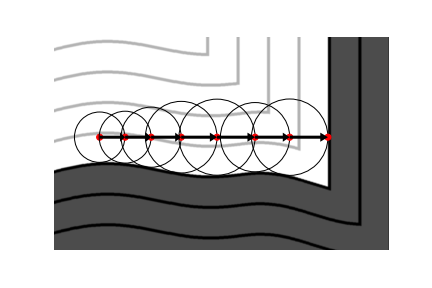
\includegraphics[scale=0.5]{img/sphereTracingViz.png}}
\caption{\label{sphereViz}{\it Visualization of the sphere tracing algorithm in 2D. A ray is sent from the source (left) to the right until it hits a surface, always moving the maximum distance as the SDF informs the tracing algorithm about the distance to the nearest surface.}}
\end{figure}

\subsection{Previous Work}
\label{ssec:prev}
A lot of previous work exists both in the field of Ray/sphere tracing and RIR estimation.
As shown in \cite{alpkocak_computing_2010} and \cite{brinkmann_round_2019} there are numerous approaches for estimating RIRs. Besides Ray-based methods such as the "Image Source Method", Ray-tracing and hybrid approaches, wave-based methods such as Finite Differences are becoming increasingly interesting due to advancements in computation power and research. Still, wave-based methods seem to be too slow for real-time applications. With the Pascal Architecture, NVIDIA introduced real-time ray tracing done on the GPU with NVIDIA VRWorks™ Audio \cite{noauthor_vrworks_nodate}.

% NVIDIA is working in the field of real time ray traced audio simulation
% NVIDIA VRWorks™ Audio (introduced with the Pascal GPU architecture) 



% \subsubsection*{RIR Estimation}
% \cite{alpkocak_computing_2010} gives an overview of methods in use for RIR estimation.


\subsubsection*{Sphere Tracing}
Sphere tracing itself was first described by \cite{hart_sphere_1996}. Since then, many authors have described improvements in speed e.g. \cite{balint_accelerating_2018} or the addition of features such as \cite{quilez_inigo_nodate}, \cite{keinert_enhanced_2014} or the activity of the \href{www.shadertoy.com}{shadertoy.com}-community.
Defining SDFs is an active field of research and there are several projects that aim at easier construction of SDFs and integration in 3D frameworks such as \href{https://github.com/Flafla2/Generic-Raymarch-Unity}{https://github.com/Flafla2/Generic-Raymarch-Unity} and \cite{lechner_hrtlacektdraymarchtoolkit_2020} but also some commercial software products have implemented raymarching and SDFs per default such as \texttt{Houdini} or \texttt{Notch}.



\subsection{Motivation}
\label{subs:mot}
The reasons why sphere tracing in a compute shader for RIR estimation has not been documented until now probably lie in the relatively new introduction of compute shaders as well as in the difficulty of creating SDFs (in comparison to using existing 3D /CAD models and importing them to polygon based ray tracers).
\subsubsection{Sphere Tracing}
As described above, ray tracing is one common method of approaching the problem of RIR estimation. Sphere tracing offers a number of advantages over ray tracing meshes or polygonal surfaces: It is procedural/parametric, by default, since all geometry is defined by implicit surface equations. Sphere tracing approximates cone tracing for reducing aliasing artifacts in the pixel domain\cite{hart_sphere_1996}. In the audio domain, beam tracing is considered to have advantages however it is is very time consuming in a non-SDF setup\cite{alpkocak_computing_2010}. Deformation and rounding of geometry is possible in a very efficient way, which might offer an opportunity to approximate low-frequency response due to diffraction artifacts. Since geometry is not defined via vertices and edges, there is no such thing as increasing the complexity of a shape in this way as in traditional mesh based approaches. Rounding a geometrical shape is a mere subtraction since it just shifts the rendering to another iso-surface which gets increasingly smooth as shown in \ref{sdf_2d_box}. Depending on the construction of the geometry, this way, holes and cavities (such as in a diffusor) can also be made to disappear for a low-frequency pass, as shown in figure \ref{fig:diffSmooth}.

\begin{figure}[ht]
\centerline{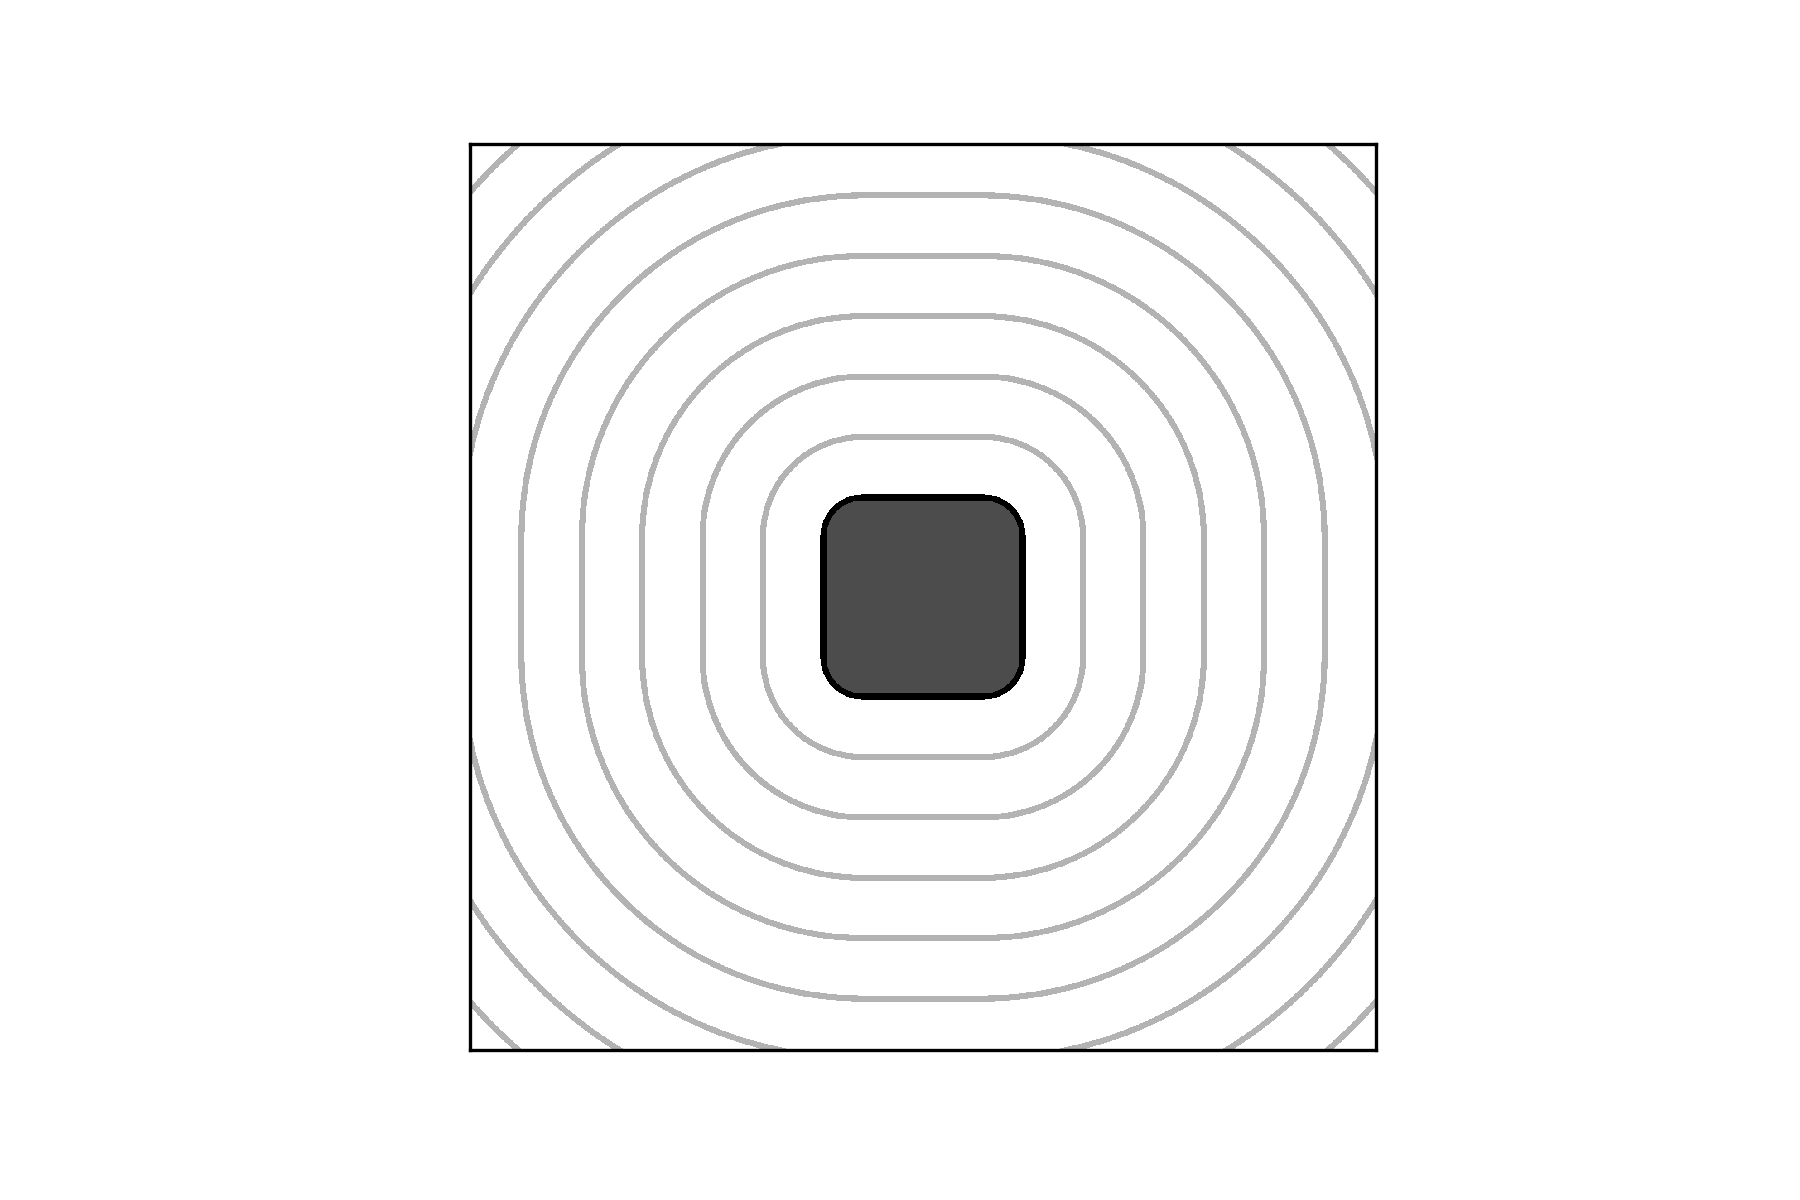
\includegraphics[scale=0.6]{img/sdf2dbox.png}}
\caption{\label{sdf_2d_box}{\it Rounding the box given in Equation \ref{eq:eq1} by subtraction of $0.7$. Visible iso-lines (gray) are generated by the distance function. The subtraction shifts the surface to a different, rounder iso-line.}}
\end{figure}  


\begin{figure}[ht]
\centering
\begin{subfigure}[t]{0.2\textwidth}
  \centering
  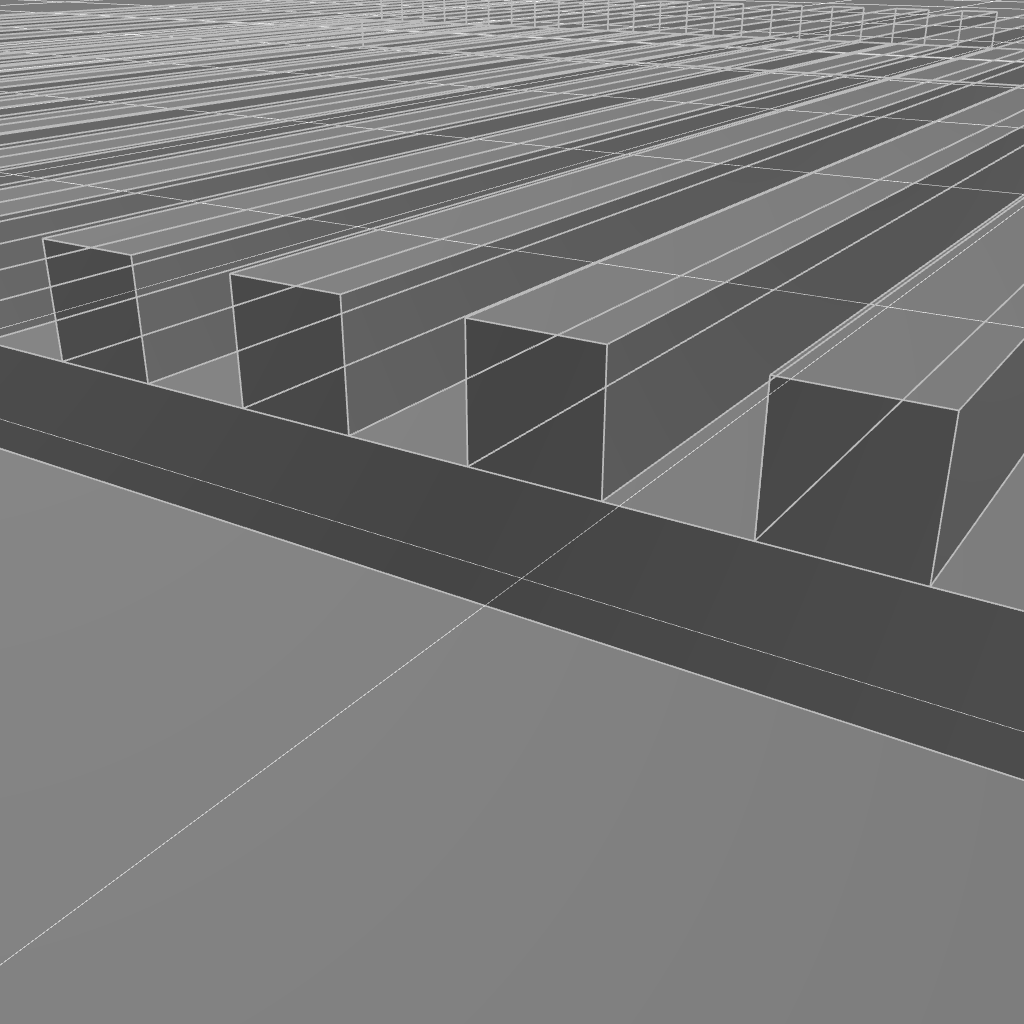
\includegraphics[width=0.9\linewidth]{img/diffusorNorm.png}
  \caption{\it Diffusor shape}
  \label{fig:diffNorm}
\end{subfigure}%
\begin{subfigure}[t]{0.2\textwidth}
  \centering
  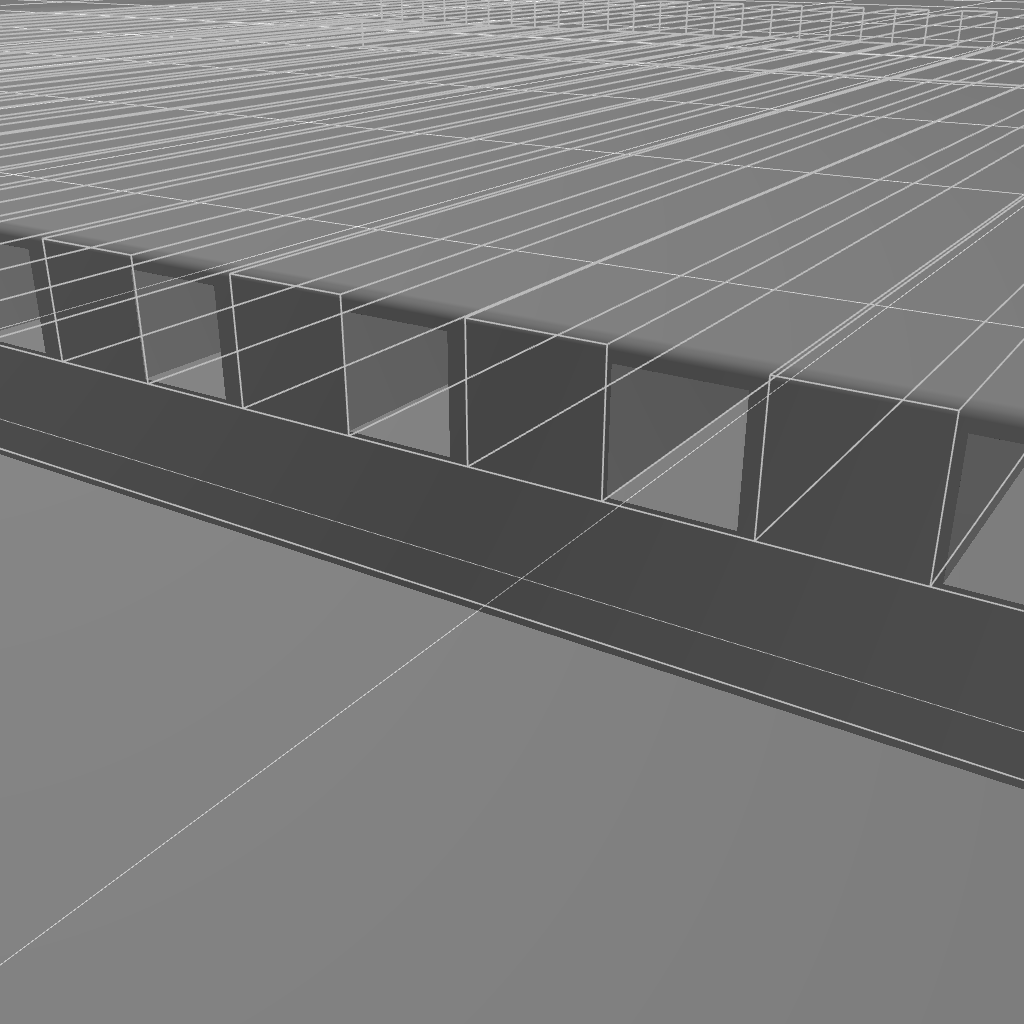
\includegraphics[width=0.9\linewidth]{img/diffusorSmooth.png}
  \caption{\it After subtraction: rounded and closed.}
  \label{fig:sub2}
\end{subfigure}
\caption{\it The diffusor from scene 1 in \cite{brinkmann_round_2019} was reconstructed exactly(a). A subtraction of $0.01$ from the distance function causes the holes to close(b).}
\label{fig:diffSmooth}
\end{figure}

\subsubsection{Implementation}
It is possible to implement the chosen algorithm on the CPU and the GPU. A number of frameworks could be chosen for GPU-accelerated computation such as OpenCL or NVIDIA CUDA. For example, \cite{stoltzfus_performance_2017} gives an overview of GPU development environments suitable for RIR estimation. The choice of a shader has the advantage of being more operating system-independent and hardware-independent as, for example, the use of CUDA ties to NVIDIA GPUs. Compute shaders (in contrast to fragment shaders) make it possible to write to arbitrary output locations which is necessary for generating the actual impulse response from the measurement of timings. Since they have been available since OpenGL 4.3 (August 2012) / OpenGL ES 3.1, they are both mature enough to have received broad support in other frameworks and relatively new in respect to first publications about sphere tracing. Another reason for the choice of compute shaders is their simplicity. In comparison to CUDA and OpenCL, shaders are easier to write and the use of the Graphics Library Shading Language (GLSL) is widespread. Achieving the whole computation, from the definition of the geometry, to the ray tracing up until the actual impulse response computation in a single shader makes this attempt highly portable and expandable.

\section{Generation of SDFs}

Only rather simplistic shapes where needed for this proof of concept. Mostly boxes were used and combined in various ways to achieve reflection areas, shoe-box scenes and the slightly more complex diffusor shape of scene 1 in \cite{brinkmann_round_2019}. A simple 3D box SDF with a size of $R_x$x$R_y$x$R_z$ can be described by:

\begin{equation}
  f(p_x, p_y, p_z) = \sqrt{c_0(p_x - R_x)^2 + c_0(p_y - R_y)^2 + c_0(p_z - R_z)^2}
  \label{eq:eq1}
\end{equation}

where $c_0$ is just clipping at 0:

\begin{equation}
c_0(x) = max(x,0) 
\end{equation}

which conveniently translates to GLSL:

\begin{lstlisting}[language=C, caption={\it GLSL code for creating a box SDF},captionpos=b, label=lst:boxSdf]
float box(vec3 pos, vec3 R){
    return length(max(abs(pos) - R,0));
}
\end{lstlisting}

\cite{hart_sphere_1996} gives a list of mathematical definitions of many shapes and for example \href{http://mercury.sexy/hg_sdf/}{http://mercury.sexy/hg\_sdf/} provides a rich and advanced library of shapes and operators that are ready to use for the creation of more complex scenery.


\section{Sphere Tracing}
For simplicity, deterministic equal-angle Ray Tracing is used in contrast to Monte Carlo or Equal Area Ray Tracing (EART) \cite{gu_room_2014}. Unidirectional ray tracing has also been used for simplicity reasons, although \cite{cao_interactive_2016} has shown that bidirectional ray tracing offers advantages. Since the classical sphere tracing algorithm was adapted, it was found to be simplest to consider the "camera" to be the receiver/microphone as it would receive light. It sends out rays that might hit the sound source which acts as a receiver of rays. The sound source is chosen to be a sphere. Choosing the correct volume for the receiver is critical and using a constant size can introduce systematic errors \cite{xiangyang_accuracy_2003}, \cite{alpkocak_computing_2010}. A number of models are available to compute the receiver volume, $V_r$. Typically factors such as room volume, the number of rays and the distance from the source are used for this computation. 
As in \cite{brandao_ray_nodate}, \cite{alpkocak_computing_2010}, and \cite{dalenback_room_1996}, the receiver was allowed to grow in volume. While \cite{brandao_ray_nodate} and \cite{dalenback_room_1996} use time as a factor to let the receiver grow, the reflection count $k$ is used in this attempt. Initially, when a ray is sent, $k=0$ and when it hits a surface, this counter is increased by one so the source grows by this factor for this particular ray. So instead of using time, the model provided in \cite{alpkocak_computing_2010} is used and augmented with the $k$ term:
\begin{equation}
V_r = (k+1) \omega d_{SR}\sqrt{\frac{4}{N}}
\end{equation}
with 
\begin{equation}
\omega = log_{10}{V_{room}}
\end{equation}
where $d_{SR}$ is the source-receiver distance, $N$ is the number of initial rays and $V_{room}$ is the volume of the room.\

The actual sphere tracing largely follows the original formulation in \cite{hart_sphere_1996} and is implemented as:

% \begin{equation}
% t_{i+1} = t_i + F(t_i)
% \end{equation}
% With $t_{i}$  being the current distance travelled along the ray being used in combination with the evaluation of the distance function $F()$ 
\begin{lstlisting}[language=C, caption={\it GLSL pseudo code for sphere tracing},captionpos=b,label=lst:sphereTrace]
for (i=0;i++;i<imax){
  vec3 pos = ro + t*rd;
  Sdf res = map(pos);
  t += res.x;
  if(res.x<epsilon){
    break
  }
}
\end{lstlisting} 

In the above simplified code listing, \texttt{ro} is a \texttt{vec3} that defines the ray origin, \texttt{rd} the ray direction and \texttt{epsilon} can be set to adjust the algorithm's precision. The \texttt{map()} function in this case not only returns the distance computed via the SDF(\texttt{res.x}) but a \texttt{struct} that can contain material properties (reflection coefficients etc.). Here it was used to distinguish between a sound source and a regular reflective body.
The space is sampled spherically and \texttt{rd} is generated from the compute shader's \

 \texttt{gl\_GlobalInvocationID}. In this implementation, a resolution of 1024 x 1024 is used, resulting in $1024^2$ initial rays and a maximum RIR length of $1024^2$.
From there, the space is sampled using the following very simplified pseudo code:
\begin{lstlisting}[language=C, caption={\it GLSL pseudo code for sampling the space and writing to the RIR.},captionpos=b, label=lst:mainloop]
Sdf res = castRay(ro,rd)
for (int k=0;k<numReflections;k++;){
  if(ComingFromReflectiveBdy){
    rd = reflect(rd,normal);
  }
  res = castRay(ro,rd);
  t = res.x;
  pos = ro+rd*t;
  if(res.body == soundSource){
    travelDistance+=t;
    readWrite(travelDistance,k);
  }
}

\end{lstlisting}

In Listing \ref{lst:mainloop}, \texttt{castRay()} refers to a function that looks similar to the sphere tracing function in Listing \ref{lst:sphereTrace} and \texttt{readWrite()} refers to a function that takes the total distance a ray has travelled from source to receiver including all reflections and the number of reflections. From the distance it computes the location where to write to in the impulse response and the attenuation. It then reads the current value at this location and adds the corresponding value, making use of a compute shader's capability to read and write its output and write to arbitrary output locations. The necessity to write to arbitrary output locations is the main reason for choosing a compute shader over a fragment shader. It is, however, possible to define most of the functionality in one file that is referenced via an \texttt{include} statement into a compute shader to calculate the RIR and into a fragment shader for visualization. This is particularly handy during the construction of geometry but also makes it possible to easily calculate the RIR of existing sphere-traced scenes for reverberation in V/A performance or other 3D video content.


\begin{figure}[ht]
\center
\begin{tikzpicture}

\node (lib) at (0,0) [rectangle,draw] {$F(p_{xyz})$};
\node (frag) at (-2,-1) [rectangle,draw] {$fragment\ shader$};
\node (comp) at (2,-1) [rectangle,draw] {$compute\ shader$};
\draw node [block, below of=frag, node distance = 1.5cm](rend){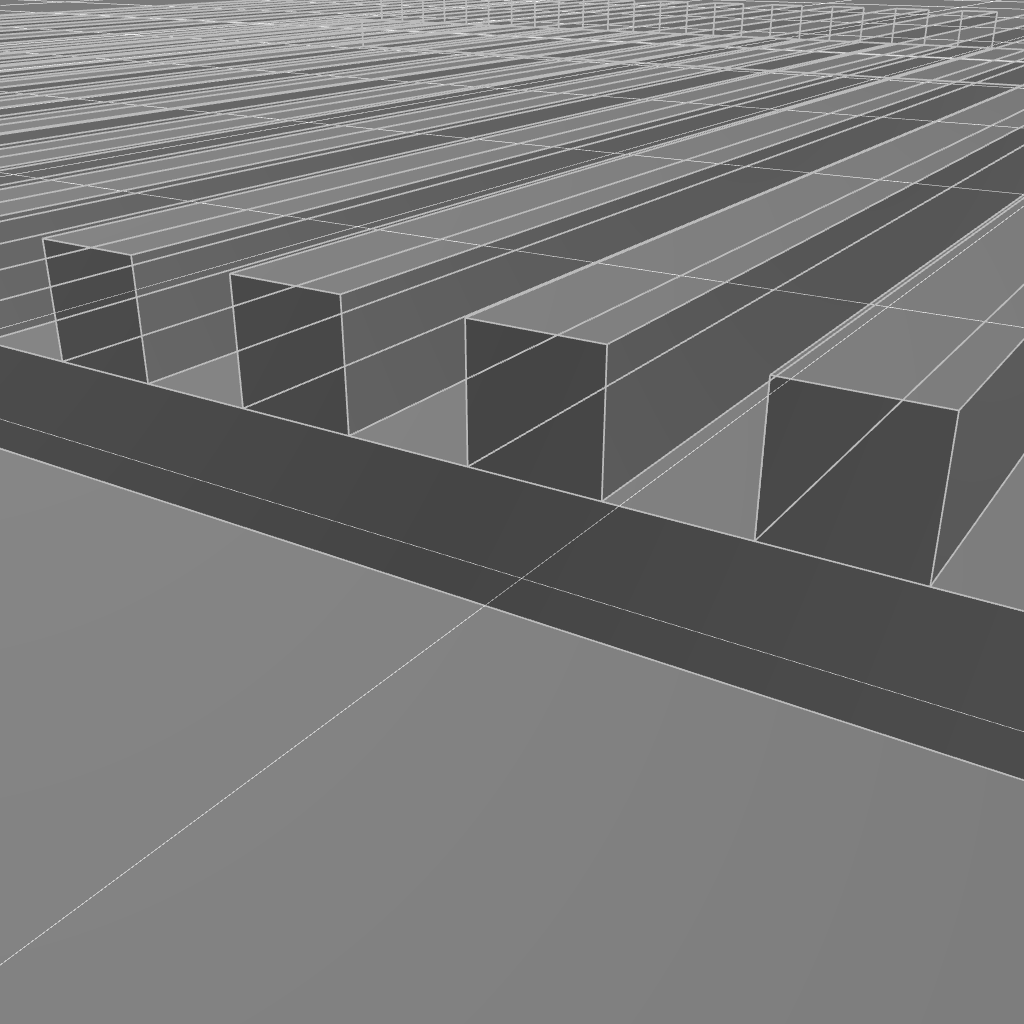
\includegraphics[width=.1\textwidth]{img/diffusorNorm.png}};
\draw node [block, below of=comp, node distance = 1.5cm](H){$H(n)$};

\draw[->] (lib) -- node {} (frag);
\draw[->] (lib) -- node {} (comp);
\draw[->] (frag) -- node {}(rend);
\draw[->] (comp) -- node {}(H);



\end{tikzpicture}
\caption{\label{fig:bd_shaders}{\it A lot of the code, especially the map function $F(p_{xyz})$ which contains the SDF, can be shared between a fragment shader used for visualization and a compute shader responsible for RIR calculation.}}
\end{figure}



% \begin{enumerate}
% \item reflection
% \item low frequency pass
% \end{enumerate}


\section{impulse response Generation}
The room is assumed to be a linear time-invariant (LTI) system. Due to the proof-of-concept nature of this proposal, a highly simplified model for RIR computation is used. Sphere tracing delivers the distances and number of reflections for $M$ rays in this implementation. Each ray follows a number of reflections $K(m)$. Each reflection pass adds up to a total travel distance of the ray, $d(m)$. The sound source is assumed to send out the discrete unit impulse function (Kronecker delta function) $\delta(n)$, see Equation \ref{equ:delta}. As non-integer delays are ignored in this implementation, the shader will just write to the rounded integer delay location $\tau_s$ in the impulse response $H(n)$ that corresponds to the distance:
\begin{equation}
\label{equ:delta}
\delta [n]={\begin{cases}1,&n=0\\0,&n\neq 0\end{cases}}\,
\end{equation}

\begin{equation}
H(n) = \sum_{m=0}^M \delta(n-\tau_s(m))\cdot \alpha(m)\cdot (-1)^{K(m)}
\end{equation}
The total attenuation per ray $\alpha(m)$ can be computed by using a material-dependent coefficient of reflection $\alpha_{mat}$ that is stored in the \texttt{Sdf struct}. At each reflection pass $k$ this results in a possibly different reflection pass-dependent coefficient $\alpha_{mat}(k,m)$ and keeping a running product in the loop of Listing \ref{lst:mainloop}:
\begin{equation}
\alpha(m)=\prod_{k=0}^{K(m)} \alpha_{mat}(k,m)
\end{equation}
For simplicity's sake, only one global coefficient $\alpha_G$ is implemented here resulting in:
\begin{equation}
\alpha(m) = \alpha_G^{K(m)}
\end{equation}

Additionally, a proof of concept for frequency-dependent loss for each reflection is introduced to the model. As a computationally efficient heuristic, a binomial filter is used \cite{aubury_binomial_1996}, \cite{derpanis_overview_nodate}. A simple one-zero filter $G(z)$ is applied for each reflection:

\begin{equation}
G(z,K) = (1+z^{-1})^K \cdot \left(\frac{1}{2}\right)^K
\end{equation}
The advantage of using such a simple filter is that a $K$-stage cascade's impulse response can be computed easily without applying the filter repeatedly. By doing the discrete time inverse Fourier transform $\mathfrak{F}^{-1}$ of the transfer function $G(z)$ the $N$-length impulse response is obtained:

\begin{equation}
  g(n,K) = \mathfrak{F}^{-1}\{ G(z) \} = \left(\frac{1}{2}\right)^K \frac{1}{N}  \sum_{\omega = 0}^\pi (1+e^{-j\omega})^{K} e^{j\omega n} 
\end{equation}
A binomial filter's impulse response converges to a Gaussian bell curve which can be approximated as:

\begin{equation}
G(n,K) \approx  \frac{1}{\sigma \cdot \sqrt{2 \pi}} \cdot e ^{-\frac{1}{2} (\frac{n-\mu}{\sigma})^2}
\label{eq:assump}
\end{equation}


with 

\begin{equation}
\sigma = \sqrt{K 0.231 + 0.562}
\end{equation}
and 
\begin{equation}
\mu = \frac{K}{2} + \frac{1}{2}
\end{equation}

The right-hand side of Equation \ref{eq:assump} is simply the normal distribution, which is computationally efficient to calculate for any $K$.

So instead of adding $\delta(n-\tau(m))$ into the RIR, $g(n-\tau(m),K)$ is simply used instead. 
Similar to many other implementations, a high-pass filter is applied to the resulting RIR to compensate for low-frequency components resulting mainly from the spacial extendedness of the sound receiver shape.

\subsubsection*{Other Frequency-Dependent Models}
Besides the faster binomial filter approach, a function for IIR filters was implemented in case a filter is needed whose Kth-order serial cascade impulse response is not known. Also, in case different materials are set up in the scene and different filters need to be applied, the binomial filter strategy is not applicable, so this approach demonstrates a more realistic scenario. The filter(s) need to be set up as sample-by-sample functions and iterated over an array. The result is inserted just as $g(n)$ above.

\subsubsection*{Output}
Following the computation of the RIR, it needs to be written to the shader's output texture. This way, an intermediate rectangular representation of N by M pixels is produced. The RIR, $h(n)$ is written to the Texture $T(x,y)$:
\begin{equation}
  T(x,y) = H(x \bmod N+\frac{y}{M})
\end{equation}

Depending on the use case (saving the RIR to a file, possible auralisation or convolution on the GPU), this data then needs to be fetched from the GPU and the process of needs to be reverted to obtain a one-dimensional signal again.


\begin{figure*}[ht]
    \center
    \begin{subfigure}[t]{0.45\textwidth}
      \centering
      % This file was created by tikzplotlib v0.9.1.
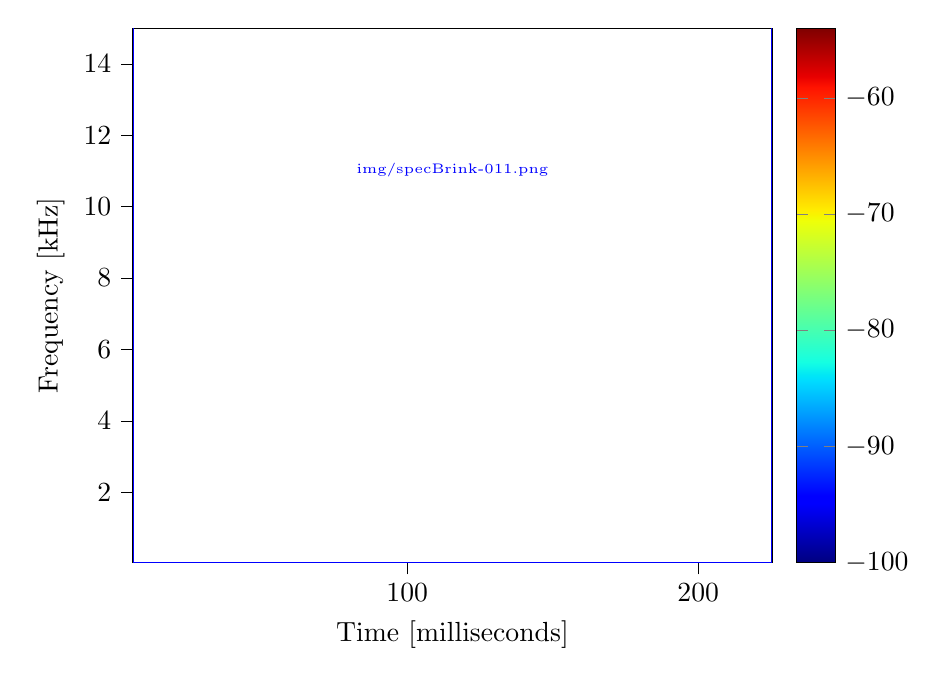
\begin{tikzpicture}

\begin{axis}[
colorbar,
colorbar style={ylabel={}, y label style={yshift=1.5em}},
colormap={mymap}{[1pt]
  rgb(0pt)=(0.0000,0.0000,0.5000);
  rgb(22pt)=(0.0000,0.0000,1.0000);
  rgb(25pt)=(0.0000,0.0000,1.0000);
  rgb(68pt)=(0.0000,0.8600,1.0000);
  rgb(70pt)=(0.0000,0.9000,0.9677);
  rgb(75pt)=(0.0806,1.0000,0.8871);
  rgb(128pt)=(0.9355,1.0000,0.0323);
  rgb(130pt)=(0.9677,0.9630,0.0000);
  rgb(132pt)=(1.0000,0.9259,0.0000);
  rgb(178pt)=(1.0000,0.0741,0.0000);
  rgb(182pt)=(0.9091,0.0000,0.0000);
  rgb(200pt)=(0.5000,0.0000,0.0000)
},
point meta max=-54.0062,
point meta min=-100.0000,
tick align=outside,
tick pos=left,
width=0.8\textwidth,
x grid style={white!69.0196!black},
xlabel={Time [milliseconds]},
xmin=0005.7, xmax=225.4,xtick={0, 100,200},
xtick style={color=black},
y grid style={white!69.0196!black},
ylabel={Frequency [kHz]},
ymin=0.0300000, ymax=15.0000000,
ytick style={color=black}
]
\addplot graphics [includegraphics cmd=\pgfimage,xmin=5.7, xmax=225.4, ymin=0.0000, ymax=22.0500000] {img/specBrink-011.png};
\end{axis}

\end{tikzpicture}

    \caption{\label{fig:fig:multReflSpecOrig} \it Original recording, scene 1, multiple reflections from \cite{brinkmann_round_2019}. }
    \end{subfigure}% 
    \begin{subfigure}[t]{0.45\textwidth}
      \centering
      % This file was created by tikzplotlib v0.9.1.
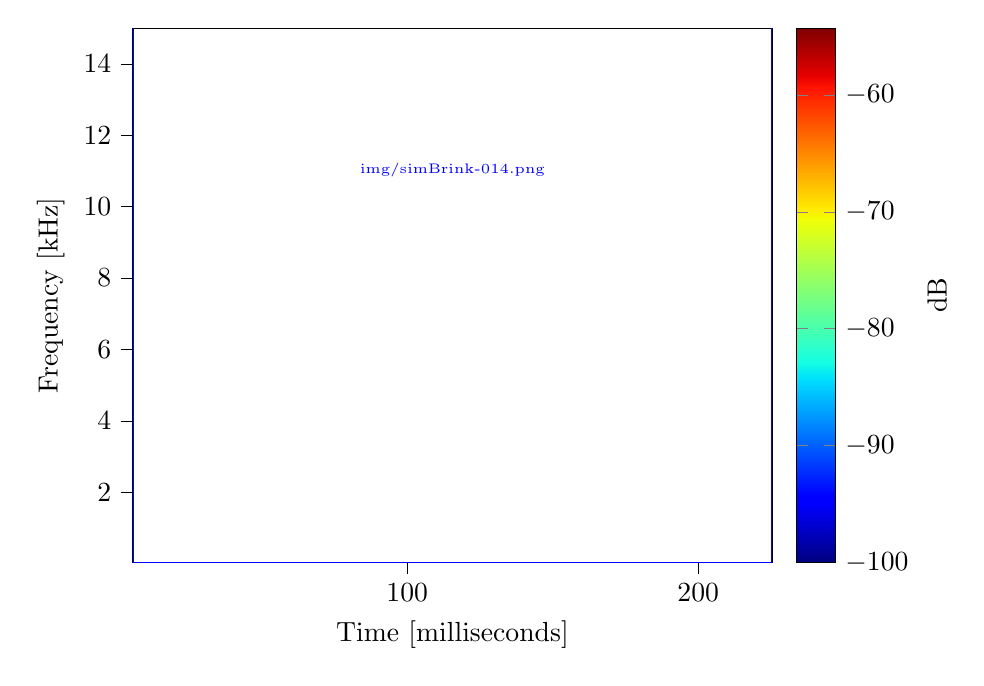
\begin{tikzpicture}

\begin{axis}[
colorbar,
colorbar style={ylabel={dB}},
colormap={mymap}{[1pt]
  rgb(0pt)=(0.0000,0.0000,0.5000);
  rgb(22pt)=(0.0000,0.0000,1.0000);
  rgb(25pt)=(0.0000,0.0000,1.0000);
  rgb(68pt)=(0.0000,0.8600,1.0000);
  rgb(70pt)=(0.0000,0.9000,0.9677);
  rgb(75pt)=(0.0806,1.0000,0.8871);
  rgb(128pt)=(0.9355,1.0000,0.0323);
  rgb(130pt)=(0.9677,0.9630,0.0000);
  rgb(132pt)=(1.0000,0.9259,0.0000);
  rgb(178pt)=(1.0000,0.0741,0.0000);
  rgb(182pt)=(0.9091,0.0000,0.0000);
  rgb(200pt)=(0.5000,0.0000,0.0000)
},
point meta max=-54.2825,
point meta min=-100.0000,
tick align=outside,
tick pos=left,
width=0.8\textwidth,
x grid style={white!69.0196!black},
xlabel={Time [milliseconds]},
xmin=005.7, xmax=225.4,xtick={100, 200},
xtick style={color=black},
y grid style={white!69.0196!black},
ylabel={Frequency [kHz]},
ymin=0.0300000, ymax=15.0000000,
ytick style={color=black}
]
\addplot graphics [includegraphics cmd=\pgfimage,xmin=5.7, xmax=225.4, ymin=0.0000, ymax=22.0500000] {img/simBrink-014.png};
\end{axis}

\end{tikzpicture}

      \caption{\label{fig:multReflSpecSim} \it Simulated using the proposed method. }
    \end{subfigure}
    \caption{\it Comparison of spectra of a real impulse response (a) and the proposed method (b).}
    \label{fig:multReflSpecCompare}
\end{figure*}


\section{Results}

\begin{figure*}[ht]
    \center
    \begin{subfigure}[t]{0.45\textwidth}
      \centering
      % This file was created by tikzplotlib v0.9.1.
\begin{tikzpicture}

\begin{axis}[
colorbar,
colorbar style={ylabel={}},
colormap={mymap}{[1pt]
  rgb(0pt)=(0.0000,0.0000,0.5000);
  rgb(22pt)=(0.0000,0.0000,1.0000);
  rgb(25pt)=(0.0000,0.0000,1.0000);
  rgb(68pt)=(0.0000,0.8600,1.0000);
  rgb(70pt)=(0.0000,0.9000,0.9677);
  rgb(75pt)=(0.0806,1.0000,0.8871);
  rgb(128pt)=(0.9355,1.0000,0.0323);
  rgb(130pt)=(0.9677,0.9630,0.0000);
  rgb(132pt)=(1.0000,0.9259,0.0000);
  rgb(178pt)=(1.0000,0.0741,0.0000);
  rgb(182pt)=(0.9091,0.0000,0.0000);
  rgb(200pt)=(0.5000,0.0000,0.0000)
},
point meta max=-54.1665,
point meta min=-100.0000,
tick align=outside,
tick pos=left,
width=0.8\textwidth,
x grid style={white!69.0196!black},
xlabel={Time [seconds]},
xmin=0.0231, xmax=0.0721,
xtick style={color=black},
y grid style={white!69.0196!black},
ylabel={Frequency [Hz]},
ymin=30.0000, ymax=5000.0000,
ytick style={color=black}
]
\addplot graphics [includegraphics cmd=\pgfimage,xmin=0.0231, xmax=0.0721, ymin=0.0000, ymax=22050.0000] {img/shoebox_orig-001.png};
\end{axis}

\end{tikzpicture}

    \caption{\label{fig:shoe} \it Spec by matlab. }
    \end{subfigure}% 
    \begin{subfigure}[t]{0.45\textwidth}
      \centering
      \input{img/shoebox_sim}
      \caption{\label{fig:shoe} \it Simulated. }
    \end{subfigure}
    \caption{\it Impulse response of shoebox room. Computed using the proposed method and \cite{lehmann_fast_2020}.}
    \label{fig:test}
\end{figure*}


All of the following results have been computed with 10 reflection passes and $1024^2$ rays. The computations were made on a strong consumer-grade machine (Intel i7 CPU, NVIDIA Geforce 1080ti). The computation time for simple scenes such as scene 1, rigid in \cite{brinkmann_round_2019} was at $<\frac{1}{60}$ seconds including the computation of a simple visualization in real time. The most complex scenes (geometrically and in regards to the amount of reflections) that where tested, the shoebox scene and scene 1 with added diffusor, where computed in less than $<\frac{1}{50}$ seconds. As expected, the method therefore outperforms CPU-based methods in computation time.  \

The results are compared to a different simulation using the image source method \cite{lehmann_fast_2020} and \cite{brinkmann_round_2019} who generated a dataset featuring recordings in in an anechoic chamber with simple shapes. Note that the comparison with \cite{brinkmann_round_2019} in figure \ref{fig:multRefl} ignores the frequency response of the speaker and microphone that were used in the original recording. As can be seen in the plot, the original recording features visible amount of difference to an ideal impulse even with the direct signal. 

Since this implementation lacks features such as material-specific reflection coefficients and passes for multiple octave bands, it is not possible to accurately compare previous work with the proposed method by simply using the same materials. It can be shown that by adjusting reflection coefficients, the method can be matched up with existing work.
Given the proof of concept nature of this proposal, there is a lot of room for improvement in terms of accuracy. More audio examples than are shown here can be inspected at the project's github repository.
\begin{figure}

    \begin{center}
      % This file was created by tikzplotlib v0.9.1.
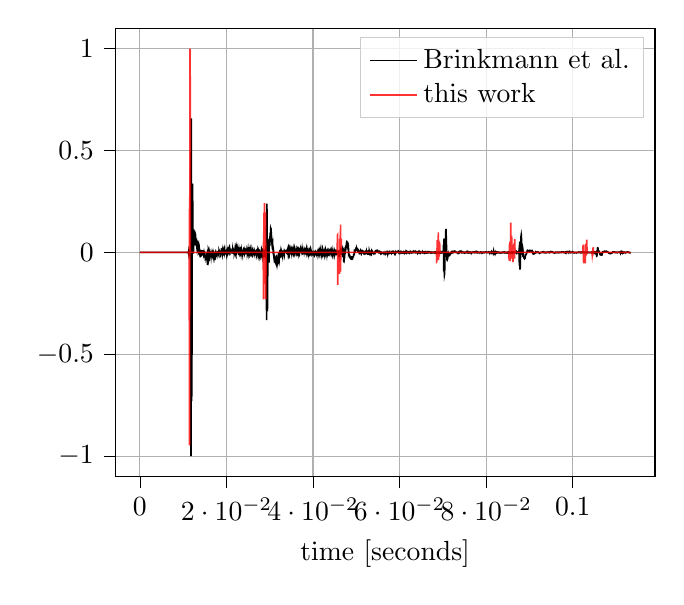
\begin{tikzpicture}

\begin{axis}[
legend cell align={left},
legend style={fill opacity=0.8, draw opacity=1, text opacity=1, draw=white!80.00000!black},
tick align=outside,
tick pos=left,
x grid style={white!69.01961!black},
xlabel={time [seconds]},
xmajorgrids,
xmin=-0.00567, xmax=0.11902,
xtick style={color=black},
y grid style={white!69.01961!black},
ymajorgrids,
ymin=-1.10000, ymax=1.10000,
ytick style={color=black}
]
\addplot [semithick, black]
table {%
0.00000 -0.00000
0.00002 0.00002
0.00005 0.00001
0.00007 0.00000
0.00009 -0.00000
0.00011 -0.00000
0.00014 0.00001
0.00016 0.00001
0.00018 0.00004
0.00020 0.00002
0.00023 0.00002
0.00025 0.00002
0.00027 0.00002
0.00029 0.00002
0.00032 -0.00001
0.00034 0.00002
0.00036 0.00000
0.00039 0.00003
0.00041 0.00003
0.00043 0.00001
0.00045 0.00002
0.00048 -0.00000
0.00050 0.00002
0.00052 0.00003
0.00054 0.00002
0.00057 0.00002
0.00059 0.00003
0.00061 0.00001
0.00063 0.00004
0.00066 0.00001
0.00068 -0.00000
0.00070 0.00003
0.00073 0.00003
0.00075 0.00001
0.00077 0.00003
0.00079 0.00004
0.00082 0.00002
0.00084 -0.00001
0.00086 0.00002
0.00088 0.00002
0.00091 0.00002
0.00093 0.00003
0.00095 0.00001
0.00098 0.00001
0.00100 0.00001
0.00102 -0.00001
0.00104 0.00003
0.00107 0.00000
0.00109 0.00001
0.00111 0.00001
0.00113 0.00003
0.00116 0.00001
0.00118 0.00001
0.00120 0.00002
0.00122 0.00002
0.00125 0.00001
0.00127 -0.00000
0.00129 0.00001
0.00132 0.00001
0.00134 0.00002
0.00136 0.00003
0.00138 0.00002
0.00141 0.00001
0.00143 0.00002
0.00145 -0.00000
0.00147 0.00001
0.00150 0.00003
0.00152 0.00003
0.00154 0.00002
0.00156 0.00001
0.00159 0.00002
0.00161 0.00002
0.00163 0.00003
0.00166 0.00004
0.00168 0.00002
0.00170 0.00003
0.00172 0.00004
0.00175 0.00002
0.00177 -0.00001
0.00179 0.00003
0.00181 0.00003
0.00184 0.00003
0.00186 0.00002
0.00188 0.00003
0.00190 0.00003
0.00193 0.00003
0.00195 0.00001
0.00197 0.00004
0.00200 -0.00000
0.00202 0.00001
0.00204 0.00004
0.00206 0.00005
0.00209 0.00001
0.00211 0.00001
0.00213 0.00004
0.00215 0.00004
0.00218 0.00000
0.00220 0.00003
0.00222 0.00001
0.00224 0.00003
0.00227 -0.00000
0.00229 0.00003
0.00231 0.00001
0.00234 0.00002
0.00236 0.00004
0.00238 -0.00000
0.00240 -0.00000
0.00243 0.00001
0.00245 0.00003
0.00247 0.00001
0.00249 0.00003
0.00252 0.00002
0.00254 0.00004
0.00256 0.00002
0.00259 0.00000
0.00261 0.00003
0.00263 0.00003
0.00265 0.00000
0.00268 0.00001
0.00270 0.00001
0.00272 -0.00002
0.00274 0.00003
0.00277 0.00005
0.00279 0.00002
0.00281 -0.00001
0.00283 -0.00001
0.00286 0.00001
0.00288 0.00003
0.00290 0.00002
0.00293 0.00002
0.00295 0.00003
0.00297 0.00006
0.00299 0.00002
0.00302 0.00001
0.00304 0.00001
0.00306 0.00001
0.00308 0.00002
0.00311 0.00002
0.00313 0.00002
0.00315 0.00002
0.00317 0.00001
0.00320 0.00005
0.00322 0.00003
0.00324 0.00004
0.00327 0.00005
0.00329 0.00002
0.00331 0.00003
0.00333 -0.00000
0.00336 0.00001
0.00338 0.00002
0.00340 0.00001
0.00342 0.00002
0.00345 0.00003
0.00347 0.00005
0.00349 0.00000
0.00351 0.00002
0.00354 0.00002
0.00356 0.00001
0.00358 0.00002
0.00361 0.00004
0.00363 0.00001
0.00365 0.00002
0.00367 0.00000
0.00370 0.00001
0.00372 0.00001
0.00374 -0.00001
0.00376 0.00002
0.00379 0.00002
0.00381 0.00004
0.00383 0.00003
0.00385 0.00002
0.00388 0.00001
0.00390 0.00001
0.00392 0.00000
0.00395 -0.00000
0.00397 -0.00002
0.00399 -0.00001
0.00401 0.00003
0.00404 0.00004
0.00406 0.00003
0.00408 -0.00002
0.00410 0.00001
0.00413 0.00002
0.00415 -0.00001
0.00417 -0.00001
0.00420 0.00002
0.00422 -0.00000
0.00424 0.00004
0.00426 0.00001
0.00429 -0.00001
0.00431 0.00001
0.00433 0.00001
0.00435 0.00002
0.00438 0.00001
0.00440 0.00001
0.00442 0.00002
0.00444 0.00004
0.00447 0.00005
0.00449 0.00003
0.00451 -0.00001
0.00454 0.00001
0.00456 0.00005
0.00458 0.00002
0.00460 0.00004
0.00463 0.00002
0.00465 0.00002
0.00467 -0.00001
0.00469 0.00002
0.00472 0.00001
0.00474 0.00001
0.00476 0.00003
0.00478 0.00001
0.00481 0.00001
0.00483 0.00002
0.00485 -0.00000
0.00488 -0.00000
0.00490 0.00001
0.00492 0.00004
0.00494 0.00003
0.00497 0.00001
0.00499 0.00000
0.00501 0.00003
0.00503 -0.00001
0.00506 0.00004
0.00508 0.00001
0.00510 -0.00002
0.00512 -0.00002
0.00515 -0.00000
0.00517 0.00001
0.00519 0.00001
0.00522 0.00001
0.00524 -0.00000
0.00526 -0.00001
0.00528 0.00003
0.00531 -0.00002
0.00533 -0.00001
0.00535 0.00003
0.00537 -0.00001
0.00540 -0.00001
0.00542 -0.00002
0.00544 -0.00001
0.00546 -0.00003
0.00549 -0.00000
0.00551 0.00001
0.00553 -0.00002
0.00556 0.00002
0.00558 -0.00001
0.00560 -0.00000
0.00562 0.00000
0.00565 -0.00000
0.00567 -0.00001
0.00569 -0.00000
0.00571 0.00002
0.00574 -0.00001
0.00576 0.00002
0.00578 0.00002
0.00580 0.00001
0.00583 -0.00003
0.00585 -0.00002
0.00587 0.00002
0.00590 -0.00002
0.00592 0.00000
0.00594 0.00001
0.00596 0.00003
0.00599 0.00002
0.00601 0.00002
0.00603 0.00003
0.00605 0.00002
0.00608 0.00001
0.00610 0.00003
0.00612 0.00003
0.00615 0.00001
0.00617 -0.00000
0.00619 0.00000
0.00621 -0.00001
0.00624 0.00001
0.00626 0.00003
0.00628 0.00001
0.00630 0.00001
0.00633 0.00001
0.00635 -0.00003
0.00637 0.00001
0.00639 -0.00001
0.00642 -0.00001
0.00644 -0.00002
0.00646 0.00000
0.00649 -0.00000
0.00651 -0.00003
0.00653 -0.00000
0.00655 -0.00002
0.00658 -0.00002
0.00660 -0.00003
0.00662 -0.00002
0.00664 -0.00004
0.00667 -0.00003
0.00669 -0.00004
0.00671 -0.00002
0.00673 0.00002
0.00676 -0.00003
0.00678 -0.00003
0.00680 -0.00006
0.00683 -0.00005
0.00685 -0.00001
0.00687 -0.00001
0.00689 -0.00000
0.00692 -0.00002
0.00694 0.00002
0.00696 0.00000
0.00698 -0.00002
0.00701 -0.00002
0.00703 -0.00001
0.00705 -0.00001
0.00707 -0.00003
0.00710 0.00000
0.00712 -0.00001
0.00714 0.00001
0.00717 0.00002
0.00719 0.00000
0.00721 0.00000
0.00723 -0.00000
0.00726 0.00001
0.00728 -0.00000
0.00730 0.00001
0.00732 0.00001
0.00735 -0.00001
0.00737 0.00001
0.00739 0.00001
0.00741 0.00003
0.00744 0.00003
0.00746 0.00002
0.00748 0.00003
0.00751 0.00001
0.00753 -0.00000
0.00755 -0.00002
0.00757 -0.00003
0.00760 -0.00002
0.00762 -0.00003
0.00764 0.00001
0.00766 0.00005
0.00769 0.00003
0.00771 0.00000
0.00773 0.00001
0.00776 -0.00004
0.00778 -0.00002
0.00780 -0.00004
0.00782 -0.00004
0.00785 -0.00002
0.00787 -0.00001
0.00789 -0.00003
0.00791 -0.00003
0.00794 -0.00003
0.00796 -0.00003
0.00798 -0.00008
0.00800 -0.00005
0.00803 -0.00007
0.00805 -0.00005
0.00807 -0.00005
0.00810 -0.00007
0.00812 -0.00008
0.00814 -0.00006
0.00816 -0.00005
0.00819 -0.00004
0.00821 -0.00003
0.00823 -0.00002
0.00825 -0.00005
0.00828 -0.00004
0.00830 -0.00003
0.00832 -0.00006
0.00834 -0.00004
0.00837 -0.00005
0.00839 -0.00003
0.00841 -0.00001
0.00844 0.00001
0.00846 -0.00000
0.00848 0.00000
0.00850 -0.00005
0.00853 -0.00002
0.00855 -0.00001
0.00857 0.00001
0.00859 -0.00000
0.00862 0.00001
0.00864 0.00001
0.00866 0.00002
0.00868 0.00000
0.00871 0.00001
0.00873 -0.00001
0.00875 -0.00001
0.00878 0.00001
0.00880 0.00002
0.00882 0.00002
0.00884 0.00001
0.00887 -0.00000
0.00889 -0.00000
0.00891 -0.00002
0.00893 0.00004
0.00896 0.00002
0.00898 -0.00001
0.00900 0.00001
0.00902 -0.00002
0.00905 -0.00006
0.00907 -0.00002
0.00909 -0.00004
0.00912 -0.00006
0.00914 -0.00007
0.00916 -0.00006
0.00918 -0.00004
0.00921 -0.00004
0.00923 -0.00004
0.00925 -0.00007
0.00927 -0.00009
0.00930 -0.00009
0.00932 -0.00012
0.00934 -0.00010
0.00937 -0.00007
0.00939 -0.00004
0.00941 -0.00005
0.00943 -0.00005
0.00946 -0.00006
0.00948 -0.00007
0.00950 -0.00013
0.00952 -0.00010
0.00955 -0.00012
0.00957 -0.00003
0.00959 -0.00009
0.00961 -0.00002
0.00964 -0.00004
0.00966 -0.00004
0.00968 -0.00005
0.00971 -0.00005
0.00973 -0.00006
0.00975 -0.00004
0.00977 -0.00004
0.00980 -0.00000
0.00982 -0.00006
0.00984 -0.00002
0.00986 -0.00003
0.00989 0.00003
0.00991 0.00001
0.00993 0.00006
0.00995 0.00004
0.00998 0.00005
0.01000 0.00002
0.01002 0.00002
0.01005 -0.00005
0.01007 -0.00000
0.01009 -0.00002
0.01011 0.00001
0.01014 0.00002
0.01016 0.00005
0.01018 0.00003
0.01020 0.00007
0.01023 0.00002
0.01025 -0.00002
0.01027 -0.00008
0.01029 -0.00007
0.01032 -0.00008
0.01034 -0.00004
0.01036 -0.00007
0.01039 -0.00001
0.01041 -0.00005
0.01043 -0.00002
0.01045 -0.00011
0.01048 -0.00009
0.01050 -0.00013
0.01052 -0.00008
0.01054 -0.00014
0.01057 -0.00007
0.01059 -0.00013
0.01061 -0.00011
0.01063 -0.00014
0.01066 -0.00012
0.01068 -0.00015
0.01070 -0.00013
0.01073 -0.00015
0.01075 -0.00014
0.01077 -0.00017
0.01079 -0.00015
0.01082 -0.00021
0.01084 -0.00017
0.01086 -0.00019
0.01088 -0.00014
0.01091 -0.00016
0.01093 -0.00008
0.01095 -0.00011
0.01098 -0.00004
0.01100 -0.00022
0.01102 -0.00005
0.01104 -0.00030
0.01107 0.00008
0.01109 -0.00028
0.01111 0.00030
0.01113 -0.00030
0.01116 0.00055
0.01118 -0.00058
0.01120 0.00084
0.01122 -0.00108
0.01125 0.00137
0.01127 -0.00162
0.01129 0.00209
0.01132 -0.00234
0.01134 0.00305
0.01136 -0.00318
0.01138 0.00427
0.01141 -0.00439
0.01143 0.00543
0.01145 -0.00583
0.01147 0.00659
0.01150 -0.00726
0.01152 0.00799
0.01154 -0.00837
0.01156 0.00913
0.01159 -0.00925
0.01161 0.01021
0.01163 -0.00982
0.01166 0.01096
0.01168 -0.01105
0.01170 0.01372
0.01172 -0.02286
0.01175 0.12720
0.01177 0.48909
0.01179 -1.00000
0.01181 -0.54537
0.01184 0.35957
0.01186 0.65806
0.01188 0.30531
0.01190 -0.14491
0.01193 -0.65035
0.01195 -0.72969
0.01197 -0.67809
0.01200 -0.63354
0.01202 -0.47761
0.01204 -0.30213
0.01206 -0.08275
0.01209 0.07996
0.01211 0.25763
0.01213 0.26513
0.01215 0.33769
0.01218 0.29233
0.01220 0.21610
0.01222 0.14696
0.01224 0.13173
0.01227 0.00715
0.01229 0.00242
0.01231 0.04460
0.01234 0.01781
0.01236 -0.00552
0.01238 0.05993
0.01240 0.06502
0.01243 0.10492
0.01245 0.11252
0.01247 0.08863
0.01249 0.08930
0.01252 0.09908
0.01254 0.06639
0.01256 0.06875
0.01259 0.05735
0.01261 0.04485
0.01263 0.05228
0.01265 0.03867
0.01268 0.03851
0.01270 0.05322
0.01272 0.05888
0.01274 0.06395
0.01277 0.07795
0.01279 0.08568
0.01281 0.08876
0.01283 0.08730
0.01286 0.07535
0.01288 0.06829
0.01290 0.05869
0.01293 0.04522
0.01295 0.04407
0.01297 0.04549
0.01299 0.04694
0.01302 0.05179
0.01304 0.05836
0.01306 0.04997
0.01308 0.05124
0.01311 0.03823
0.01313 0.03124
0.01315 0.02773
0.01317 0.03060
0.01320 0.02267
0.01322 0.03934
0.01324 0.02850
0.01327 0.03187
0.01329 0.05743
0.01331 0.03062
0.01333 0.03909
0.01336 0.02586
0.01338 0.02263
0.01340 0.02365
0.01342 0.02529
0.01345 0.01631
0.01347 0.01864
0.01349 0.02177
0.01351 0.01916
0.01354 0.02254
0.01356 0.01075
0.01358 0.00621
0.01361 0.02949
0.01363 0.01520
0.01365 0.01684
0.01367 -0.00864
0.01370 0.01046
0.01372 0.02259
0.01374 0.01801
0.01376 0.00017
0.01379 -0.00467
0.01381 -0.00500
0.01383 -0.01384
0.01385 0.00254
0.01388 0.01324
0.01390 -0.01411
0.01392 -0.02451
0.01395 0.00383
0.01397 -0.00636
0.01399 0.01127
0.01401 -0.01329
0.01404 0.00659
0.01406 0.00274
0.01408 0.00868
0.01410 0.00007
0.01413 0.00104
0.01415 -0.00477
0.01417 -0.01021
0.01420 -0.01754
0.01422 -0.00484
0.01424 -0.01491
0.01426 -0.00098
0.01429 -0.00583
0.01431 -0.00465
0.01433 0.00222
0.01435 -0.00709
0.01438 0.01032
0.01440 0.00325
0.01442 -0.00005
0.01444 0.01103
0.01447 -0.00969
0.01449 0.00605
0.01451 0.00949
0.01454 -0.00527
0.01456 0.00339
0.01458 -0.01581
0.01460 0.00217
0.01463 -0.00374
0.01465 -0.00976
0.01467 -0.00065
0.01469 0.00001
0.01472 -0.00480
0.01474 0.00272
0.01476 -0.00401
0.01478 -0.00199
0.01481 -0.00667
0.01483 0.00778
0.01485 -0.01235
0.01488 -0.00181
0.01490 0.00589
0.01492 -0.01087
0.01494 0.00190
0.01497 -0.00853
0.01499 -0.01512
0.01501 0.00232
0.01503 -0.02296
0.01506 -0.02425
0.01508 -0.01132
0.01510 -0.02081
0.01512 -0.01954
0.01515 -0.01112
0.01517 -0.03033
0.01519 -0.02646
0.01522 -0.01842
0.01524 -0.02199
0.01526 -0.01917
0.01528 -0.02779
0.01531 -0.03243
0.01533 -0.03747
0.01535 -0.02350
0.01537 -0.01504
0.01540 -0.02931
0.01542 -0.02521
0.01544 -0.03762
0.01546 -0.01476
0.01549 -0.03252
0.01551 -0.00230
0.01553 -0.02400
0.01556 -0.00370
0.01558 -0.01251
0.01560 -0.06212
0.01562 -0.00811
0.01565 0.01206
0.01567 0.00847
0.01569 -0.02792
0.01571 -0.02972
0.01574 -0.02790
0.01576 -0.02004
0.01578 -0.00253
0.01580 0.01045
0.01583 0.00808
0.01585 -0.00251
0.01587 -0.01384
0.01590 -0.02034
0.01592 -0.02833
0.01594 -0.02579
0.01596 -0.02873
0.01599 -0.02980
0.01601 -0.01801
0.01603 -0.01158
0.01605 -0.00365
0.01608 -0.01730
0.01610 -0.00492
0.01612 -0.00720
0.01615 -0.01133
0.01617 -0.02040
0.01619 -0.01158
0.01621 -0.00811
0.01624 -0.02370
0.01626 -0.00716
0.01628 -0.01569
0.01630 -0.01072
0.01633 -0.02417
0.01635 -0.00463
0.01637 -0.01048
0.01639 -0.01259
0.01642 -0.01770
0.01644 -0.01219
0.01646 -0.01428
0.01649 -0.02380
0.01651 -0.01321
0.01653 -0.00903
0.01655 -0.01816
0.01658 -0.01881
0.01660 -0.01575
0.01662 -0.02185
0.01664 -0.01313
0.01667 -0.02527
0.01669 -0.01499
0.01671 -0.01004
0.01673 -0.01441
0.01676 -0.01873
0.01678 -0.01985
0.01680 -0.01719
0.01683 -0.01378
0.01685 -0.02175
0.01687 -0.01004
0.01689 -0.01139
0.01692 -0.01294
0.01694 -0.01452
0.01696 -0.01451
0.01698 -0.01690
0.01701 -0.00763
0.01703 -0.01504
0.01705 -0.00871
0.01707 -0.01306
0.01710 -0.00815
0.01712 -0.00951
0.01714 -0.00808
0.01717 -0.01087
0.01719 -0.00310
0.01721 -0.01654
0.01723 -0.00142
0.01726 -0.00697
0.01728 -0.01243
0.01730 -0.00932
0.01732 -0.00908
0.01735 -0.00825
0.01737 -0.01227
0.01739 -0.01774
0.01741 -0.00543
0.01744 -0.00389
0.01746 -0.00877
0.01748 -0.00641
0.01751 -0.00985
0.01753 -0.00611
0.01755 -0.00588
0.01757 -0.00510
0.01760 -0.01802
0.01762 0.00384
0.01764 -0.00298
0.01766 -0.00657
0.01769 -0.01307
0.01771 -0.00762
0.01773 -0.00497
0.01776 -0.00521
0.01778 -0.00694
0.01780 0.00030
0.01782 -0.00893
0.01785 -0.00302
0.01787 -0.00289
0.01789 -0.00487
0.01791 -0.01262
0.01794 -0.00787
0.01796 -0.00887
0.01798 -0.00819
0.01800 -0.00432
0.01803 -0.00545
0.01805 -0.01175
0.01807 -0.00771
0.01810 0.00066
0.01812 -0.00615
0.01814 -0.00706
0.01816 -0.00917
0.01819 -0.01090
0.01821 -0.00474
0.01823 -0.00091
0.01825 -0.00251
0.01828 -0.00996
0.01830 0.00352
0.01832 0.00188
0.01834 -0.00321
0.01837 -0.00339
0.01839 -0.00957
0.01841 0.00103
0.01844 -0.00093
0.01846 -0.00227
0.01848 -0.00228
0.01850 -0.00333
0.01853 -0.00936
0.01855 0.00599
0.01857 -0.00269
0.01859 -0.00688
0.01862 0.00237
0.01864 -0.00527
0.01866 -0.00406
0.01868 -0.00604
0.01871 -0.00197
0.01873 -0.00383
0.01875 -0.00234
0.01878 -0.01102
0.01880 -0.00068
0.01882 0.00468
0.01884 -0.00203
0.01887 -0.00443
0.01889 -0.00758
0.01891 0.00105
0.01893 -0.00004
0.01896 0.00321
0.01898 0.00090
0.01900 -0.00657
0.01902 0.00650
0.01905 0.00058
0.01907 0.00338
0.01909 -0.00214
0.01912 0.00237
0.01914 -0.00156
0.01916 0.00311
0.01918 0.00420
0.01921 0.00236
0.01923 0.00735
0.01925 -0.00515
0.01927 0.00824
0.01930 0.00581
0.01932 0.00117
0.01934 0.00048
0.01937 0.00590
0.01939 0.00486
0.01941 0.00264
0.01943 0.00260
0.01946 0.00681
0.01948 0.00417
0.01950 0.00127
0.01952 0.00313
0.01955 0.00800
0.01957 0.00186
0.01959 0.00401
0.01961 0.00705
0.01964 0.00016
0.01966 0.00082
0.01968 0.00102
0.01971 0.00786
0.01973 0.00079
0.01975 0.00171
0.01977 0.00858
0.01980 0.00327
0.01982 0.00100
0.01984 0.00041
0.01986 0.00098
0.01989 0.00117
0.01991 0.00117
0.01993 0.00232
0.01995 -0.00019
0.01998 0.00784
0.02000 -0.00369
0.02002 0.00490
0.02005 0.00655
0.02007 0.00033
0.02009 0.00178
0.02011 -0.00174
0.02014 0.00394
0.02016 -0.00338
0.02018 0.01074
0.02020 0.00525
0.02023 -0.01436
0.02025 0.01160
0.02027 0.01379
0.02029 0.01330
0.02032 0.01220
0.02034 0.01071
0.02036 -0.00191
0.02039 -0.00014
0.02041 0.00055
0.02043 0.00886
0.02045 0.00742
0.02048 0.01114
0.02050 0.00978
0.02052 0.00331
0.02054 0.01601
0.02057 0.00751
0.02059 0.01195
0.02061 0.00443
0.02063 0.01245
0.02066 0.00296
0.02068 0.00867
0.02070 0.00629
0.02073 0.01051
0.02075 0.00194
0.02077 0.00762
0.02079 0.01121
0.02082 0.00746
0.02084 0.00584
0.02086 0.00947
0.02088 0.00744
0.02091 0.00833
0.02093 0.00697
0.02095 0.00163
0.02098 0.00875
0.02100 0.00258
0.02102 0.00805
0.02104 0.00317
0.02107 -0.00146
0.02109 0.01155
0.02111 0.00765
0.02113 0.00486
0.02116 0.00457
0.02118 0.00585
0.02120 0.00381
0.02122 0.00462
0.02125 0.00363
0.02127 0.00721
0.02129 0.01034
0.02132 0.01082
0.02134 0.00840
0.02136 0.00169
0.02138 0.01041
0.02141 0.00412
0.02143 0.00930
0.02145 0.00576
0.02147 0.00621
0.02150 0.00452
0.02152 0.00660
0.02154 0.00531
0.02156 -0.00032
0.02159 0.00884
0.02161 0.00976
0.02163 0.00105
0.02166 0.00998
0.02168 0.00102
0.02170 0.00812
0.02172 0.00868
0.02175 0.01169
0.02177 0.01260
0.02179 0.01214
0.02181 0.00113
0.02184 0.00439
0.02186 0.01556
0.02188 0.00502
0.02190 0.01051
0.02193 0.00330
0.02195 0.01178
0.02197 0.00533
0.02200 0.00757
0.02202 0.00512
0.02204 0.01225
0.02206 0.01003
0.02209 0.00478
0.02211 0.00039
0.02213 0.01013
0.02215 0.00640
0.02218 0.00448
0.02220 0.00972
0.02222 0.00690
0.02224 0.00395
0.02227 0.01307
0.02229 0.01011
0.02231 0.00431
0.02234 0.00836
0.02236 0.00011
0.02238 0.00756
0.02240 0.00718
0.02243 0.01012
0.02245 0.00084
0.02247 0.00434
0.02249 0.01181
0.02252 0.00757
0.02254 0.00899
0.02256 0.00411
0.02259 0.00986
0.02261 0.00777
0.02263 0.00158
0.02265 0.00804
0.02268 0.00990
0.02270 0.00633
0.02272 0.00548
0.02274 0.00733
0.02277 0.00687
0.02279 0.00649
0.02281 0.00713
0.02283 0.00632
0.02286 0.01064
0.02288 0.00196
0.02290 0.00295
0.02293 0.01072
0.02295 0.00817
0.02297 0.00623
0.02299 0.00285
0.02302 0.00584
0.02304 0.00593
0.02306 0.01011
0.02308 0.01107
0.02311 0.00588
0.02313 0.00707
0.02315 0.00364
0.02317 0.00458
0.02320 0.01215
0.02322 0.00544
0.02324 0.00741
0.02327 0.00296
0.02329 0.00121
0.02331 0.01196
0.02333 0.00568
0.02336 0.00581
0.02338 0.00261
0.02340 0.00627
0.02342 0.00074
0.02345 0.00573
0.02347 0.01036
0.02349 0.00781
0.02351 0.00183
0.02354 0.00093
0.02356 0.00182
0.02358 0.00476
0.02361 0.00310
0.02363 0.00668
0.02365 0.00650
0.02367 0.00055
0.02370 -0.00351
0.02372 0.00501
0.02374 0.01106
0.02376 0.00348
0.02379 0.00384
0.02381 0.00232
0.02383 0.00394
0.02385 0.00101
0.02388 0.00308
0.02390 0.00324
0.02392 0.00198
0.02395 0.00461
0.02397 0.00100
0.02399 0.00693
0.02401 0.00801
0.02404 0.00436
0.02406 0.00223
0.02408 0.00784
0.02410 0.00413
0.02413 0.00223
0.02415 0.00627
0.02417 0.00411
0.02420 0.00490
0.02422 0.00628
0.02424 0.00457
0.02426 0.00548
0.02429 0.01076
0.02431 0.00416
0.02433 0.00295
0.02435 0.00378
0.02438 0.00601
0.02440 0.00418
0.02442 0.00587
0.02444 0.00453
0.02447 0.00362
0.02449 0.00435
0.02451 -0.00333
0.02454 0.00814
0.02456 0.01203
0.02458 -0.00794
0.02460 0.00481
0.02463 0.00337
0.02465 0.00409
0.02467 0.00678
0.02469 0.00335
0.02472 0.00206
0.02474 0.00205
0.02476 0.00603
0.02478 0.00043
0.02481 0.00498
0.02483 0.00634
0.02485 0.00144
0.02488 0.00431
0.02490 -0.00297
0.02492 0.00163
0.02494 0.00181
0.02497 0.00685
0.02499 0.00148
0.02501 0.00116
0.02503 0.00545
0.02506 0.00488
0.02508 -0.00045
0.02510 0.00234
0.02512 0.00139
0.02515 0.00490
0.02517 0.00487
0.02519 0.00194
0.02522 -0.00073
0.02524 0.00084
0.02526 0.00415
0.02528 0.00250
0.02531 0.00405
0.02533 0.00094
0.02535 0.00374
0.02537 0.00091
0.02540 0.00186
0.02542 0.00514
0.02544 0.00011
0.02546 0.00235
0.02549 -0.00136
0.02551 -0.00054
0.02553 0.00389
0.02556 0.00167
0.02558 -0.00000
0.02560 0.00363
0.02562 0.00183
0.02565 0.00196
0.02567 -0.00178
0.02569 -0.00051
0.02571 0.00367
0.02574 -0.00208
0.02576 -0.00075
0.02578 -0.00218
0.02580 0.00547
0.02583 0.00099
0.02585 -0.00012
0.02587 0.00138
0.02590 0.00141
0.02592 -0.00217
0.02594 -0.00375
0.02596 0.00284
0.02599 0.00197
0.02601 -0.00159
0.02603 -0.00227
0.02605 0.00408
0.02608 0.00154
0.02610 -0.00362
0.02612 -0.00506
0.02615 -0.00169
0.02617 0.00098
0.02619 -0.00150
0.02621 -0.00254
0.02624 -0.00285
0.02626 0.00108
0.02628 0.00070
0.02630 -0.00156
0.02633 -0.00295
0.02635 -0.00082
0.02637 0.00201
0.02639 0.00105
0.02642 0.00025
0.02644 -0.00267
0.02646 -0.00298
0.02649 -0.00568
0.02651 -0.00003
0.02653 0.00280
0.02655 0.00071
0.02658 -0.00226
0.02660 -0.00359
0.02662 -0.00341
0.02664 -0.00117
0.02667 -0.00141
0.02669 -0.00552
0.02671 -0.00453
0.02673 -0.00066
0.02676 0.00056
0.02678 -0.00606
0.02680 -0.00028
0.02683 0.00121
0.02685 -0.01007
0.02687 -0.00006
0.02689 0.00106
0.02692 -0.00113
0.02694 -0.00130
0.02696 -0.00496
0.02698 -0.00353
0.02701 -0.00612
0.02703 -0.00021
0.02705 -0.00589
0.02707 -0.00350
0.02710 0.00357
0.02712 0.00462
0.02714 -0.00634
0.02717 -0.00559
0.02719 0.00198
0.02721 0.00536
0.02723 0.00255
0.02726 -0.01926
0.02728 -0.00508
0.02730 -0.00297
0.02732 -0.00432
0.02735 -0.00590
0.02737 -0.00813
0.02739 0.00155
0.02741 -0.00442
0.02744 -0.00873
0.02746 -0.01079
0.02748 -0.00104
0.02751 -0.00373
0.02753 -0.00046
0.02755 0.00061
0.02757 -0.00541
0.02760 -0.00288
0.02762 0.00025
0.02764 0.00758
0.02766 0.00192
0.02769 -0.00597
0.02771 -0.01538
0.02773 -0.01400
0.02776 -0.00046
0.02778 0.00312
0.02780 0.00426
0.02782 0.00436
0.02785 0.00167
0.02787 0.00172
0.02789 -0.00415
0.02791 -0.00129
0.02794 0.00065
0.02796 -0.00231
0.02798 -0.00389
0.02800 -0.00098
0.02803 -0.00633
0.02805 -0.00648
0.02807 -0.00796
0.02810 -0.00295
0.02812 -0.00555
0.02814 -0.00198
0.02816 -0.00594
0.02819 -0.00708
0.02821 -0.00058
0.02823 0.00304
0.02825 -0.00251
0.02828 -0.00509
0.02830 0.00035
0.02832 -0.00443
0.02834 -0.00404
0.02837 -0.00147
0.02839 -0.00151
0.02841 -0.00536
0.02844 -0.01775
0.02846 -0.01570
0.02848 0.00389
0.02850 0.00295
0.02853 -0.00057
0.02855 -0.01003
0.02857 -0.01273
0.02859 -0.01801
0.02862 -0.01712
0.02864 -0.01052
0.02866 -0.00636
0.02868 0.00030
0.02871 0.00283
0.02873 0.01291
0.02875 0.00174
0.02878 -0.00537
0.02880 -0.01442
0.02882 -0.00996
0.02884 -0.01155
0.02887 -0.00698
0.02889 -0.00509
0.02891 -0.00310
0.02893 -0.00444
0.02896 0.00011
0.02898 -0.00429
0.02900 0.00417
0.02902 -0.00404
0.02905 0.00284
0.02907 0.00395
0.02909 0.00419
0.02912 -0.00607
0.02914 0.00091
0.02916 -0.01248
0.02918 0.00307
0.02921 -0.00997
0.02923 0.06554
0.02925 0.12807
0.02927 -0.33225
0.02930 -0.21590
0.02932 0.10223
0.02934 0.23898
0.02937 0.11844
0.02939 -0.05220
0.02941 -0.25081
0.02943 -0.28865
0.02946 -0.27854
0.02948 -0.25152
0.02950 -0.19971
0.02952 -0.11500
0.02955 -0.02673
0.02957 0.02377
0.02959 0.06365
0.02961 0.05389
0.02964 0.06162
0.02966 0.03712
0.02968 0.01484
0.02971 -0.02077
0.02973 -0.04892
0.02975 -0.01886
0.02977 -0.00627
0.02980 -0.02722
0.02982 -0.05021
0.02984 -0.01960
0.02986 0.03893
0.02989 0.04916
0.02991 0.06861
0.02993 0.04166
0.02995 0.04080
0.02998 0.03082
0.03000 0.05792
0.03002 0.05891
0.03005 0.06322
0.03007 0.07543
0.03009 0.08774
0.03011 0.09639
0.03014 0.08023
0.03016 0.08307
0.03018 0.08554
0.03020 0.10441
0.03023 0.11772
0.03025 0.11643
0.03027 0.11970
0.03029 0.10260
0.03032 0.10333
0.03034 0.09399
0.03036 0.07565
0.03039 0.08128
0.03041 0.07086
0.03043 0.06302
0.03045 0.05690
0.03048 0.05006
0.03050 0.04596
0.03052 0.04861
0.03054 0.04719
0.03057 0.05294
0.03059 0.05256
0.03061 0.04450
0.03063 0.04248
0.03066 0.04511
0.03068 0.03439
0.03070 0.02916
0.03073 0.02155
0.03075 0.01544
0.03077 0.01268
0.03079 0.00334
0.03082 -0.00314
0.03084 -0.01013
0.03086 -0.00243
0.03088 -0.00964
0.03091 -0.01035
0.03093 -0.01410
0.03095 -0.01020
0.03098 -0.01629
0.03100 -0.02187
0.03102 -0.02281
0.03104 -0.02447
0.03107 -0.02233
0.03109 -0.02330
0.03111 -0.02785
0.03113 -0.02901
0.03116 -0.02259
0.03118 -0.03302
0.03120 -0.03182
0.03122 -0.03518
0.03125 -0.03571
0.03127 -0.04393
0.03129 -0.03646
0.03132 -0.04152
0.03134 -0.04402
0.03136 -0.04599
0.03138 -0.04442
0.03141 -0.04695
0.03143 -0.04413
0.03145 -0.04726
0.03147 -0.04614
0.03150 -0.04617
0.03152 -0.04251
0.03154 -0.04539
0.03156 -0.04842
0.03159 -0.04437
0.03161 -0.05248
0.03163 -0.05847
0.03166 -0.04584
0.03168 -0.05125
0.03170 -0.05102
0.03172 -0.04520
0.03175 -0.05336
0.03177 -0.05082
0.03179 -0.04764
0.03181 -0.04337
0.03184 -0.04017
0.03186 -0.03339
0.03188 -0.03112
0.03190 -0.04042
0.03193 -0.03502
0.03195 -0.03294
0.03197 -0.03271
0.03200 -0.03178
0.03202 -0.03401
0.03204 -0.02955
0.03206 -0.02891
0.03209 -0.03023
0.03211 -0.03015
0.03213 -0.01807
0.03215 -0.02537
0.03218 -0.02973
0.03220 -0.02224
0.03222 -0.01696
0.03224 -0.01833
0.03227 -0.01150
0.03229 -0.01168
0.03231 -0.02301
0.03234 -0.01250
0.03236 0.00060
0.03238 -0.00004
0.03240 -0.00835
0.03243 -0.01532
0.03245 -0.01605
0.03247 -0.01357
0.03249 -0.00675
0.03252 -0.00066
0.03254 0.00240
0.03256 -0.00142
0.03259 -0.00997
0.03261 -0.01118
0.03263 -0.01473
0.03265 -0.01834
0.03268 -0.01781
0.03270 -0.01807
0.03272 -0.01559
0.03274 -0.01486
0.03277 -0.00669
0.03279 -0.00892
0.03281 -0.00849
0.03283 -0.01131
0.03286 -0.01005
0.03288 -0.01217
0.03290 -0.01007
0.03293 -0.00831
0.03295 -0.01004
0.03297 -0.00850
0.03299 -0.01166
0.03302 -0.00496
0.03304 -0.00590
0.03306 -0.00849
0.03308 -0.01046
0.03311 -0.00723
0.03313 -0.00791
0.03315 -0.00860
0.03317 -0.00826
0.03320 -0.00542
0.03322 -0.01069
0.03324 -0.00480
0.03327 -0.00162
0.03329 -0.00128
0.03331 -0.00559
0.03333 -0.00515
0.03336 -0.00257
0.03338 -0.00502
0.03340 0.00096
0.03342 0.00565
0.03345 0.00532
0.03347 0.00226
0.03349 0.00281
0.03351 0.00470
0.03354 0.00561
0.03356 0.00541
0.03358 0.00535
0.03361 0.00701
0.03363 0.00675
0.03365 0.00390
0.03367 0.00358
0.03370 0.00563
0.03372 0.01145
0.03374 0.00755
0.03376 0.00673
0.03379 0.00719
0.03381 0.00470
0.03383 0.00378
0.03385 0.00407
0.03388 0.00742
0.03390 0.00808
0.03392 0.00228
0.03395 0.00331
0.03397 -0.00086
0.03399 0.00390
0.03401 0.00771
0.03404 0.00950
0.03406 0.01098
0.03408 0.01013
0.03410 0.00918
0.03413 0.01180
0.03415 0.00309
0.03417 0.00393
0.03420 0.00634
0.03422 0.00222
0.03424 0.00600
0.03426 0.00476
0.03429 0.00819
0.03431 -0.00020
0.03433 -0.00202
0.03435 0.00520
0.03438 0.00404
0.03440 0.00449
0.03442 0.00040
0.03444 0.00364
0.03447 0.00457
0.03449 0.00746
0.03451 0.00397
0.03454 0.00675
0.03456 0.00381
0.03458 0.00879
0.03460 0.01078
0.03463 0.01013
0.03465 0.01078
0.03467 0.01056
0.03469 0.01281
0.03472 0.00976
0.03474 0.01310
0.03476 0.01075
0.03478 0.01022
0.03481 0.01147
0.03483 0.00520
0.03485 0.00954
0.03488 0.01292
0.03490 0.01276
0.03492 0.01020
0.03494 0.01057
0.03497 0.01261
0.03499 0.00731
0.03501 0.00463
0.03503 0.01250
0.03506 0.01420
0.03508 0.00764
0.03510 0.01083
0.03512 0.01035
0.03515 0.00966
0.03517 0.00814
0.03519 0.01128
0.03522 0.00887
0.03524 0.00999
0.03526 0.01129
0.03528 0.01228
0.03531 0.00755
0.03533 0.00767
0.03535 0.02064
0.03537 0.01152
0.03540 0.00648
0.03542 0.00919
0.03544 0.00897
0.03546 0.00661
0.03549 0.00898
0.03551 0.01162
0.03553 0.00712
0.03556 0.01131
0.03558 0.01026
0.03560 0.00633
0.03562 0.00595
0.03565 0.01161
0.03567 0.00372
0.03569 0.00102
0.03571 0.00417
0.03574 0.00537
0.03576 0.01139
0.03578 0.00902
0.03580 0.01035
0.03583 0.00707
0.03585 0.00636
0.03587 0.00677
0.03590 0.00518
0.03592 0.00972
0.03594 0.00824
0.03596 0.00836
0.03599 0.00930
0.03601 0.00613
0.03603 0.00851
0.03605 0.00911
0.03608 0.00574
0.03610 0.00618
0.03612 0.00408
0.03615 0.00625
0.03617 0.00447
0.03619 0.00461
0.03621 0.00627
0.03624 0.00424
0.03626 -0.00059
0.03628 0.00096
0.03630 0.00757
0.03633 0.00466
0.03635 0.00502
0.03637 0.00528
0.03639 0.00256
0.03642 0.00200
0.03644 0.00450
0.03646 0.00079
0.03649 0.00311
0.03651 0.00405
0.03653 0.00148
0.03655 0.00312
0.03658 0.00132
0.03660 0.00480
0.03662 0.00447
0.03664 -0.00026
0.03667 0.00365
0.03669 0.00389
0.03671 0.00547
0.03673 0.00703
0.03676 0.00431
0.03678 0.01055
0.03680 0.00936
0.03683 0.00842
0.03685 0.00500
0.03687 0.00505
0.03689 0.00638
0.03692 0.00777
0.03694 0.00907
0.03696 0.00522
0.03698 0.00781
0.03701 0.01079
0.03703 0.00847
0.03705 0.00774
0.03707 0.00756
0.03710 0.01166
0.03712 0.00857
0.03714 0.00880
0.03717 0.00940
0.03719 0.00859
0.03721 0.01123
0.03723 0.01155
0.03726 0.00982
0.03728 0.00973
0.03730 0.00947
0.03732 0.00821
0.03735 0.01096
0.03737 0.00832
0.03739 0.00371
0.03741 0.00419
0.03744 0.00380
0.03746 0.00740
0.03748 0.00239
0.03751 0.00415
0.03753 0.00844
0.03755 0.00782
0.03757 0.00637
0.03760 0.00305
0.03762 0.00200
0.03764 0.00440
0.03766 0.00678
0.03769 0.00127
0.03771 0.00224
0.03773 0.00313
0.03776 0.00297
0.03778 0.00400
0.03780 0.00410
0.03782 0.00385
0.03785 0.00476
0.03787 0.00296
0.03789 0.00348
0.03791 0.00495
0.03794 0.00523
0.03796 0.00218
0.03798 0.00463
0.03800 0.00317
0.03803 0.00285
0.03805 0.00600
0.03807 0.00541
0.03810 0.00304
0.03812 -0.00030
0.03814 0.00594
0.03816 0.00449
0.03819 0.00714
0.03821 0.00500
0.03823 -0.00143
0.03825 0.00590
0.03828 0.00610
0.03830 0.00147
0.03832 0.00236
0.03834 0.00240
0.03837 -0.00114
0.03839 -0.00206
0.03841 0.00291
0.03844 0.00339
0.03846 0.00363
0.03848 0.00157
0.03850 0.00632
0.03853 0.00101
0.03855 -0.00090
0.03857 0.00211
0.03859 -0.00004
0.03862 -0.00005
0.03864 -0.00166
0.03866 -0.00024
0.03868 -0.00141
0.03871 -0.00002
0.03873 -0.00039
0.03875 -0.00105
0.03878 0.00247
0.03880 -0.00045
0.03882 -0.00403
0.03884 0.00136
0.03887 -0.00247
0.03889 -0.00074
0.03891 -0.00417
0.03893 -0.00121
0.03896 -0.00098
0.03898 -0.00272
0.03900 -0.00042
0.03902 -0.00024
0.03905 -0.00063
0.03907 -0.00052
0.03909 0.00123
0.03912 0.00010
0.03914 0.00214
0.03916 -0.00109
0.03918 -0.00411
0.03921 -0.00194
0.03923 0.00070
0.03925 0.00269
0.03927 0.00227
0.03930 0.00051
0.03932 -0.00170
0.03934 -0.00051
0.03937 0.00353
0.03939 -0.00036
0.03941 -0.00117
0.03943 -0.00239
0.03946 -0.00349
0.03948 -0.00114
0.03950 0.00221
0.03952 -0.00103
0.03955 0.00096
0.03957 0.00019
0.03959 -0.00507
0.03961 -0.00027
0.03964 -0.00250
0.03966 0.00018
0.03968 -0.00146
0.03971 -0.00239
0.03973 -0.00252
0.03975 -0.00582
0.03977 -0.00463
0.03980 0.00291
0.03982 0.00247
0.03984 0.00117
0.03986 -0.00177
0.03989 -0.00265
0.03991 -0.00294
0.03993 -0.00199
0.03995 -0.00085
0.03998 -0.00166
0.04000 -0.00402
0.04002 -0.00303
0.04005 -0.00199
0.04007 -0.00211
0.04009 -0.00343
0.04011 -0.00438
0.04014 -0.00447
0.04016 -0.00193
0.04018 -0.00226
0.04020 -0.00462
0.04023 -0.00150
0.04025 -0.00238
0.04027 -0.00499
0.04029 -0.00453
0.04032 -0.00314
0.04034 -0.00505
0.04036 -0.00189
0.04039 -0.00259
0.04041 -0.00472
0.04043 -0.00397
0.04045 -0.00153
0.04048 -0.00193
0.04050 -0.00257
0.04052 -0.00137
0.04054 -0.00395
0.04057 -0.00230
0.04059 -0.00210
0.04061 -0.00209
0.04063 -0.00279
0.04066 -0.00230
0.04068 -0.00192
0.04070 -0.00646
0.04073 0.00095
0.04075 0.00022
0.04077 -0.00479
0.04079 -0.00427
0.04082 -0.00676
0.04084 -0.00438
0.04086 -0.00518
0.04088 -0.00486
0.04091 -0.00451
0.04093 -0.00373
0.04095 -0.00361
0.04098 -0.00085
0.04100 -0.00114
0.04102 -0.00239
0.04104 -0.00414
0.04107 -0.00522
0.04109 -0.00492
0.04111 -0.00114
0.04113 -0.00255
0.04116 -0.00104
0.04118 -0.00624
0.04120 -0.00375
0.04122 -0.00564
0.04125 -0.00192
0.04127 -0.00017
0.04129 -0.00553
0.04132 -0.00651
0.04134 -0.00725
0.04136 -0.00757
0.04138 -0.00502
0.04141 -0.00353
0.04143 -0.00237
0.04145 -0.00167
0.04147 -0.00539
0.04150 -0.00776
0.04152 -0.00238
0.04154 0.00048
0.04156 -0.00275
0.04159 -0.00334
0.04161 0.00052
0.04163 0.00293
0.04166 -0.01305
0.04168 -0.00731
0.04170 0.00706
0.04172 -0.00398
0.04175 -0.00881
0.04177 -0.00066
0.04179 -0.01056
0.04181 -0.00655
0.04184 0.00148
0.04186 -0.00038
0.04188 -0.00603
0.04190 -0.00832
0.04193 -0.00188
0.04195 0.00617
0.04197 0.00922
0.04200 0.01043
0.04202 0.01081
0.04204 0.00849
0.04206 0.00786
0.04209 -0.00139
0.04211 0.00430
0.04213 0.00123
0.04215 -0.00251
0.04218 -0.00287
0.04220 -0.00281
0.04222 -0.00092
0.04224 -0.00559
0.04227 -0.00281
0.04229 0.00119
0.04231 0.00888
0.04234 0.00641
0.04236 -0.00093
0.04238 -0.00372
0.04240 -0.00360
0.04243 -0.00687
0.04245 -0.00594
0.04247 -0.00748
0.04249 -0.00224
0.04252 -0.00125
0.04254 -0.00356
0.04256 0.00490
0.04259 -0.00073
0.04261 -0.01210
0.04263 0.00076
0.04265 0.01033
0.04268 0.01024
0.04270 -0.00531
0.04272 -0.00967
0.04274 -0.00313
0.04277 -0.00587
0.04279 -0.00201
0.04281 -0.00269
0.04283 0.00053
0.04286 0.00265
0.04288 0.00673
0.04290 0.00438
0.04293 -0.00248
0.04295 0.00209
0.04297 0.01122
0.04299 0.00996
0.04302 0.00859
0.04304 -0.00001
0.04306 -0.00333
0.04308 -0.00220
0.04311 -0.00254
0.04313 -0.00052
0.04315 0.00046
0.04317 -0.00289
0.04320 0.00562
0.04322 0.01033
0.04324 0.00602
0.04327 0.00117
0.04329 0.00071
0.04331 0.00642
0.04333 0.00097
0.04336 0.00238
0.04338 -0.00117
0.04340 0.00090
0.04342 -0.00177
0.04345 -0.00283
0.04347 0.00226
0.04349 0.00088
0.04351 0.00266
0.04354 -0.00166
0.04356 -0.00028
0.04358 0.00166
0.04361 0.00018
0.04363 0.00340
0.04365 0.00292
0.04367 -0.00028
0.04370 0.00180
0.04372 0.00301
0.04374 0.00042
0.04376 0.00036
0.04379 -0.00120
0.04381 -0.00190
0.04383 -0.00343
0.04385 -0.00138
0.04388 -0.00078
0.04390 -0.00047
0.04392 0.00108
0.04395 0.00113
0.04397 0.00283
0.04399 0.00149
0.04401 -0.00305
0.04404 -0.00103
0.04406 0.00353
0.04408 0.00273
0.04410 -0.00235
0.04413 -0.00657
0.04415 0.00240
0.04417 0.00096
0.04420 -0.00032
0.04422 -0.00197
0.04424 -0.00148
0.04426 -0.00213
0.04429 0.00203
0.04431 -0.00112
0.04433 0.00105
0.04435 -0.00127
0.04438 -0.00279
0.04440 0.00413
0.04442 0.00408
0.04444 0.00171
0.04447 -0.00056
0.04449 -0.00034
0.04451 -0.00496
0.04454 -0.00138
0.04456 -0.00035
0.04458 -0.00004
0.04460 -0.00213
0.04463 0.00568
0.04465 0.00350
0.04467 0.00140
0.04469 -0.00099
0.04472 0.00152
0.04474 0.00048
0.04476 0.00020
0.04478 -0.00208
0.04481 0.00028
0.04483 0.00113
0.04485 -0.00168
0.04488 -0.00049
0.04490 -0.00081
0.04492 -0.00239
0.04494 -0.00105
0.04497 0.00069
0.04499 -0.00301
0.04501 0.00077
0.04503 -0.00140
0.04506 -0.00323
0.04508 -0.00132
0.04510 -0.00132
0.04512 -0.00127
0.04515 0.00016
0.04517 -0.00335
0.04519 -0.00278
0.04522 0.00268
0.04524 0.00247
0.04526 -0.00331
0.04528 -0.00543
0.04531 -0.00452
0.04533 -0.00520
0.04535 -0.00158
0.04537 -0.00165
0.04540 0.00073
0.04542 0.00008
0.04544 -0.00074
0.04546 -0.00052
0.04549 0.00153
0.04551 -0.00039
0.04553 -0.00129
0.04556 -0.00256
0.04558 -0.00219
0.04560 -0.00028
0.04562 -0.00101
0.04565 -0.00046
0.04567 -0.00126
0.04569 -0.00095
0.04571 -0.00203
0.04574 -0.00086
0.04576 0.00069
0.04578 0.00125
0.04580 -0.00109
0.04583 -0.00474
0.04585 -0.00207
0.04587 0.00021
0.04590 -0.00003
0.04592 -0.00164
0.04594 -0.00210
0.04596 -0.00295
0.04599 -0.00086
0.04601 -0.00001
0.04603 -0.00253
0.04605 -0.00110
0.04608 -0.00119
0.04610 -0.00073
0.04612 -0.00030
0.04615 -0.00062
0.04617 -0.00229
0.04619 -0.00674
0.04621 -0.00299
0.04624 -0.00037
0.04626 0.00097
0.04628 -0.00080
0.04630 -0.00135
0.04633 -0.00342
0.04635 -0.00791
0.04637 -0.00254
0.04639 -0.00406
0.04642 -0.00368
0.04644 -0.00104
0.04646 0.00351
0.04649 0.00050
0.04651 -0.01227
0.04653 -0.00365
0.04655 0.00299
0.04658 0.00235
0.04660 -0.00023
0.04662 -0.00091
0.04664 0.00381
0.04667 0.00649
0.04669 0.00328
0.04671 0.00623
0.04673 0.00354
0.04676 0.00079
0.04678 0.00534
0.04680 -0.00095
0.04683 -0.00139
0.04685 0.00206
0.04687 -0.00141
0.04689 -0.00137
0.04692 -0.00504
0.04694 -0.01061
0.04696 -0.00548
0.04698 0.00061
0.04701 -0.00148
0.04703 0.00035
0.04705 -0.00732
0.04707 -0.02612
0.04710 -0.03783
0.04712 -0.04446
0.04714 -0.04491
0.04717 -0.04052
0.04719 -0.03502
0.04721 -0.03132
0.04723 -0.03064
0.04726 -0.02690
0.04728 -0.01698
0.04730 -0.00868
0.04732 -0.00066
0.04735 0.00309
0.04737 -0.00142
0.04739 -0.00177
0.04741 0.00226
0.04744 0.00682
0.04746 0.00743
0.04748 0.00481
0.04751 0.00788
0.04753 0.01122
0.04755 0.01356
0.04757 0.01592
0.04760 0.02092
0.04762 0.02451
0.04764 0.02725
0.04766 0.02844
0.04769 0.03256
0.04771 0.03805
0.04773 0.04381
0.04776 0.04721
0.04778 0.05197
0.04780 0.05284
0.04782 0.05213
0.04785 0.05043
0.04787 0.04901
0.04789 0.04723
0.04791 0.04310
0.04794 0.04147
0.04796 0.03871
0.04798 0.03517
0.04800 0.03162
0.04803 0.02912
0.04805 0.02628
0.04807 0.02738
0.04810 0.02558
0.04812 0.02460
0.04814 0.01898
0.04816 0.01227
0.04819 0.01637
0.04821 0.01018
0.04823 0.00703
0.04825 -0.00062
0.04828 -0.00768
0.04830 -0.01037
0.04832 -0.01389
0.04834 -0.01488
0.04837 -0.01583
0.04839 -0.01706
0.04841 -0.01708
0.04844 -0.02047
0.04846 -0.02136
0.04848 -0.01971
0.04850 -0.01873
0.04853 -0.02089
0.04855 -0.02068
0.04857 -0.02097
0.04859 -0.02068
0.04862 -0.02135
0.04864 -0.02253
0.04866 -0.02441
0.04868 -0.02659
0.04871 -0.02756
0.04873 -0.02902
0.04875 -0.02857
0.04878 -0.02904
0.04880 -0.02953
0.04882 -0.02836
0.04884 -0.02842
0.04887 -0.02672
0.04889 -0.02358
0.04891 -0.02261
0.04893 -0.02265
0.04896 -0.02475
0.04898 -0.02349
0.04900 -0.02375
0.04902 -0.02440
0.04905 -0.02574
0.04907 -0.02739
0.04909 -0.02676
0.04912 -0.02682
0.04914 -0.02647
0.04916 -0.02744
0.04918 -0.02604
0.04921 -0.02331
0.04923 -0.02303
0.04925 -0.02107
0.04927 -0.02073
0.04930 -0.02066
0.04932 -0.01939
0.04934 -0.01855
0.04937 -0.01658
0.04939 -0.01291
0.04941 -0.01065
0.04943 -0.01016
0.04946 -0.01031
0.04948 -0.00822
0.04950 -0.00483
0.04952 -0.00657
0.04955 -0.00703
0.04957 -0.00243
0.04959 -0.00131
0.04961 -0.00080
0.04964 -0.00010
0.04966 0.00398
0.04968 0.00567
0.04971 0.00883
0.04973 0.00859
0.04975 0.01032
0.04977 0.01140
0.04980 0.01067
0.04982 0.01298
0.04984 0.01443
0.04986 0.01365
0.04989 0.01508
0.04991 0.01510
0.04993 0.01525
0.04995 0.01688
0.04998 0.01682
0.05000 0.01849
0.05002 0.01540
0.05005 0.01643
0.05007 0.01695
0.05009 0.01759
0.05011 0.01571
0.05014 0.01476
0.05016 0.01450
0.05018 0.01509
0.05020 0.01419
0.05023 0.01352
0.05025 0.01310
0.05027 0.01191
0.05029 0.01264
0.05032 0.01039
0.05034 0.00776
0.05036 0.00676
0.05039 0.00720
0.05041 0.00954
0.05043 0.00908
0.05045 0.00608
0.05048 0.00493
0.05050 0.00453
0.05052 0.00565
0.05054 0.00395
0.05057 0.00347
0.05059 0.00141
0.05061 0.00010
0.05063 -0.00089
0.05066 0.00152
0.05068 0.00152
0.05070 0.00065
0.05073 -0.00048
0.05075 -0.00089
0.05077 -0.00139
0.05079 -0.00040
0.05082 0.00032
0.05084 0.00151
0.05086 0.00273
0.05088 0.00141
0.05091 0.00323
0.05093 0.00279
0.05095 0.00303
0.05098 0.00181
0.05100 0.00384
0.05102 0.00214
0.05104 0.00235
0.05107 0.00469
0.05109 0.00586
0.05111 0.00581
0.05113 0.00311
0.05116 0.00576
0.05118 0.00629
0.05120 0.00529
0.05122 0.00345
0.05125 0.00718
0.05127 0.00736
0.05129 0.00482
0.05132 0.00505
0.05134 0.00494
0.05136 0.00372
0.05138 0.00348
0.05141 0.00466
0.05143 0.00373
0.05145 0.00488
0.05147 0.00442
0.05150 0.00407
0.05152 0.00612
0.05154 0.00567
0.05156 0.00477
0.05159 0.00474
0.05161 0.00318
0.05163 0.00286
0.05166 0.00286
0.05168 0.00139
0.05170 0.00141
0.05172 -0.00059
0.05175 0.00058
0.05177 -0.00092
0.05179 -0.00091
0.05181 -0.00034
0.05184 -0.00034
0.05186 -0.00100
0.05188 -0.00312
0.05190 -0.00236
0.05193 -0.00135
0.05195 -0.00179
0.05197 -0.00202
0.05200 -0.00045
0.05202 -0.00003
0.05204 -0.00066
0.05206 -0.00240
0.05209 -0.00174
0.05211 -0.00033
0.05213 -0.00111
0.05215 0.00027
0.05218 -0.00133
0.05220 0.00011
0.05222 0.00007
0.05224 -0.00010
0.05227 0.00097
0.05229 0.00004
0.05231 0.00010
0.05234 0.00090
0.05236 0.00003
0.05238 -0.00065
0.05240 0.00359
0.05243 0.00113
0.05245 -0.00025
0.05247 -0.00156
0.05249 -0.00148
0.05252 0.00024
0.05254 0.00031
0.05256 0.00044
0.05259 0.00037
0.05261 -0.00012
0.05263 0.00541
0.05265 -0.00186
0.05268 -0.01186
0.05270 0.00183
0.05272 0.00932
0.05274 0.00496
0.05277 0.00073
0.05279 -0.00622
0.05281 -0.01176
0.05283 -0.00658
0.05286 -0.00251
0.05288 -0.00182
0.05290 0.00153
0.05293 0.00325
0.05295 0.00269
0.05297 0.00686
0.05299 0.00480
0.05302 0.00137
0.05304 0.00068
0.05306 0.00017
0.05308 -0.00048
0.05311 -0.00296
0.05313 -0.00158
0.05315 0.00070
0.05317 0.00120
0.05320 -0.00027
0.05322 -0.00151
0.05324 -0.00280
0.05327 0.00059
0.05329 0.00136
0.05331 0.00179
0.05333 0.00113
0.05336 0.00239
0.05338 0.00325
0.05340 0.00255
0.05342 -0.00067
0.05345 -0.00277
0.05347 -0.00049
0.05349 0.00140
0.05351 -0.00108
0.05354 -0.00240
0.05356 -0.00012
0.05358 0.00056
0.05361 0.00058
0.05363 0.00039
0.05365 0.00196
0.05367 0.00155
0.05370 0.00261
0.05372 0.00042
0.05374 -0.00073
0.05376 -0.00165
0.05379 -0.00238
0.05381 -0.00268
0.05383 -0.00242
0.05385 -0.00326
0.05388 -0.00321
0.05390 -0.00336
0.05392 -0.00267
0.05395 -0.00227
0.05397 -0.00330
0.05399 -0.00444
0.05401 -0.00497
0.05404 -0.00324
0.05406 -0.00342
0.05408 -0.00518
0.05410 -0.00476
0.05413 -0.00276
0.05415 -0.00322
0.05417 -0.00169
0.05420 -0.00120
0.05422 -0.00043
0.05424 0.00108
0.05426 0.00103
0.05429 0.00138
0.05431 0.00217
0.05433 0.00053
0.05435 0.00064
0.05438 0.00147
0.05440 0.00200
0.05442 0.00052
0.05444 0.00142
0.05447 0.00223
0.05449 0.00401
0.05451 0.00451
0.05454 0.00396
0.05456 0.00454
0.05458 0.00412
0.05460 0.00444
0.05463 0.00550
0.05465 0.00471
0.05467 0.00436
0.05469 0.00508
0.05472 0.00384
0.05474 0.00383
0.05476 0.00500
0.05478 0.00416
0.05481 0.00429
0.05483 0.00345
0.05485 0.00336
0.05488 0.00417
0.05490 0.00488
0.05492 0.00548
0.05494 0.00282
0.05497 0.00270
0.05499 0.00404
0.05501 0.00298
0.05503 0.00206
0.05506 0.00237
0.05508 0.00192
0.05510 0.00243
0.05512 0.00253
0.05515 0.00154
0.05517 0.00205
0.05519 0.00158
0.05522 0.00033
0.05524 0.00106
0.05526 -0.00072
0.05528 -0.00083
0.05531 -0.00074
0.05533 -0.00048
0.05535 -0.00133
0.05537 -0.00171
0.05540 -0.00137
0.05542 -0.00006
0.05544 -0.00074
0.05546 -0.00101
0.05549 0.00014
0.05551 -0.00020
0.05553 -0.00145
0.05556 -0.00281
0.05558 -0.00095
0.05560 -0.00147
0.05562 -0.00106
0.05565 -0.00107
0.05567 -0.00102
0.05569 -0.00104
0.05571 -0.00168
0.05574 -0.00169
0.05576 0.00005
0.05578 -0.00037
0.05580 -0.00059
0.05583 -0.00245
0.05585 -0.00164
0.05587 -0.00092
0.05590 -0.00093
0.05592 -0.00178
0.05594 -0.00171
0.05596 -0.00120
0.05599 -0.00162
0.05601 -0.00200
0.05603 -0.00254
0.05605 -0.00207
0.05608 -0.00174
0.05610 -0.00280
0.05612 -0.00289
0.05615 -0.00212
0.05617 -0.00189
0.05619 -0.00158
0.05621 -0.00268
0.05624 -0.00321
0.05626 -0.00322
0.05628 -0.00265
0.05630 -0.00279
0.05633 -0.00239
0.05635 -0.00353
0.05637 -0.00262
0.05639 -0.00204
0.05642 -0.00291
0.05644 -0.00340
0.05646 -0.00449
0.05649 -0.00421
0.05651 -0.00448
0.05653 -0.00373
0.05655 -0.00418
0.05658 -0.00388
0.05660 -0.00372
0.05662 -0.00322
0.05664 -0.00450
0.05667 -0.00190
0.05669 -0.00280
0.05671 -0.00417
0.05673 -0.00291
0.05676 -0.00298
0.05678 -0.00432
0.05680 -0.00420
0.05683 -0.00387
0.05685 -0.00361
0.05687 -0.00203
0.05689 -0.00234
0.05692 -0.00295
0.05694 -0.00182
0.05696 -0.00128
0.05698 -0.00329
0.05701 -0.00342
0.05703 -0.00229
0.05705 -0.00367
0.05707 -0.00312
0.05710 -0.00243
0.05712 -0.00259
0.05714 -0.00242
0.05717 -0.00109
0.05719 -0.00240
0.05721 -0.00297
0.05723 -0.00023
0.05726 -0.00109
0.05728 -0.00455
0.05730 -0.00280
0.05732 -0.00251
0.05735 -0.00317
0.05737 -0.00291
0.05739 -0.00222
0.05741 -0.00275
0.05744 -0.00203
0.05746 -0.00218
0.05748 -0.00163
0.05751 -0.00189
0.05753 -0.00101
0.05755 -0.00224
0.05757 -0.00317
0.05760 -0.00242
0.05762 -0.00285
0.05764 -0.00295
0.05766 -0.00272
0.05769 -0.00314
0.05771 -0.00342
0.05773 -0.00334
0.05776 -0.00267
0.05778 -0.00121
0.05780 -0.00256
0.05782 -0.00221
0.05785 -0.00244
0.05787 -0.00282
0.05789 -0.00311
0.05791 -0.00307
0.05794 -0.00311
0.05796 -0.00342
0.05798 -0.00324
0.05800 -0.00247
0.05803 -0.00136
0.05805 -0.00105
0.05807 -0.00118
0.05810 -0.00122
0.05812 -0.00051
0.05814 -0.00241
0.05816 -0.00345
0.05819 -0.00166
0.05821 -0.00104
0.05823 -0.00050
0.05825 -0.00310
0.05828 -0.00265
0.05830 -0.00050
0.05832 -0.00085
0.05834 -0.00100
0.05837 -0.00152
0.05839 -0.00097
0.05841 -0.00163
0.05844 -0.00138
0.05846 -0.00137
0.05848 -0.00115
0.05850 0.00017
0.05853 -0.00126
0.05855 -0.00133
0.05857 -0.00013
0.05859 -0.00115
0.05862 -0.00059
0.05864 0.00057
0.05866 0.00006
0.05868 -0.00075
0.05871 -0.00091
0.05873 -0.00083
0.05875 0.00099
0.05878 0.00076
0.05880 0.00014
0.05882 -0.00149
0.05884 0.00017
0.05887 0.00038
0.05889 0.00040
0.05891 0.00086
0.05893 0.00085
0.05896 0.00008
0.05898 0.00075
0.05900 0.00029
0.05902 -0.00122
0.05905 0.00188
0.05907 0.00111
0.05909 0.00140
0.05912 -0.00023
0.05914 -0.00013
0.05916 0.00066
0.05918 0.00049
0.05921 0.00029
0.05923 0.00059
0.05925 -0.00053
0.05927 -0.00019
0.05930 0.00125
0.05932 0.00097
0.05934 0.00176
0.05937 0.00184
0.05939 0.00269
0.05941 0.00272
0.05943 0.00313
0.05946 0.00341
0.05948 0.00298
0.05950 0.00281
0.05952 0.00361
0.05955 0.00335
0.05957 0.00387
0.05959 0.00248
0.05961 0.00223
0.05964 0.00236
0.05966 0.00299
0.05968 0.00307
0.05971 0.00229
0.05973 0.00130
0.05975 0.00157
0.05977 0.00241
0.05980 0.00076
0.05982 0.00172
0.05984 0.00168
0.05986 0.00218
0.05989 0.00059
0.05991 0.00061
0.05993 -0.00057
0.05995 0.00046
0.05998 0.00098
0.06000 0.00068
0.06002 -0.00020
0.06005 -0.00010
0.06007 -0.00102
0.06009 -0.00113
0.06011 0.00149
0.06014 0.00180
0.06016 0.00044
0.06018 0.00031
0.06020 0.00115
0.06023 0.00002
0.06025 0.00109
0.06027 0.00074
0.06029 0.00051
0.06032 -0.00090
0.06034 0.00006
0.06036 -0.00119
0.06039 -0.00067
0.06041 0.00088
0.06043 0.00107
0.06045 0.00004
0.06048 -0.00076
0.06050 -0.00099
0.06052 0.00104
0.06054 0.00082
0.06057 -0.00089
0.06059 -0.00076
0.06061 -0.00042
0.06063 -0.00007
0.06066 -0.00054
0.06068 -0.00088
0.06070 0.00022
0.06073 0.00033
0.06075 0.00047
0.06077 -0.00070
0.06079 -0.00077
0.06082 -0.00032
0.06084 0.00075
0.06086 0.00012
0.06088 -0.00175
0.06091 -0.00169
0.06093 -0.00046
0.06095 -0.00054
0.06098 -0.00029
0.06100 0.00075
0.06102 0.00012
0.06104 0.00040
0.06107 -0.00139
0.06109 -0.00007
0.06111 0.00093
0.06113 0.00055
0.06116 -0.00019
0.06118 -0.00074
0.06120 -0.00062
0.06122 -0.00055
0.06125 0.00028
0.06127 0.00099
0.06129 0.00132
0.06132 0.00114
0.06134 -0.00053
0.06136 -0.00018
0.06138 0.00027
0.06141 -0.00044
0.06143 0.00119
0.06145 0.00007
0.06147 -0.00047
0.06150 -0.00031
0.06152 -0.00016
0.06154 -0.00092
0.06156 0.00060
0.06159 0.00197
0.06161 0.00054
0.06163 -0.00032
0.06166 0.00053
0.06168 -0.00015
0.06170 -0.00067
0.06172 0.00007
0.06175 -0.00047
0.06177 -0.00035
0.06179 -0.00047
0.06181 -0.00014
0.06184 0.00001
0.06186 0.00059
0.06188 0.00008
0.06190 0.00029
0.06193 0.00057
0.06195 0.00147
0.06197 0.00091
0.06200 -0.00031
0.06202 0.00044
0.06204 0.00059
0.06206 0.00060
0.06209 0.00040
0.06211 0.00093
0.06213 0.00131
0.06215 0.00102
0.06218 0.00024
0.06220 0.00093
0.06222 0.00049
0.06224 0.00118
0.06227 0.00002
0.06229 -0.00069
0.06231 0.00087
0.06234 0.00095
0.06236 0.00035
0.06238 0.00047
0.06240 0.00033
0.06243 0.00095
0.06245 0.00154
0.06247 0.00211
0.06249 0.00093
0.06252 0.00047
0.06254 0.00113
0.06256 0.00100
0.06259 0.00110
0.06261 0.00056
0.06263 0.00139
0.06265 0.00087
0.06268 0.00073
0.06270 0.00090
0.06272 0.00018
0.06274 0.00111
0.06277 0.00146
0.06279 0.00003
0.06281 0.00024
0.06283 0.00036
0.06286 0.00076
0.06288 0.00032
0.06290 0.00046
0.06293 0.00032
0.06295 0.00046
0.06297 0.00038
0.06299 0.00084
0.06302 0.00155
0.06304 0.00208
0.06306 0.00125
0.06308 0.00037
0.06311 0.00110
0.06313 0.00117
0.06315 0.00089
0.06317 0.00115
0.06320 0.00188
0.06322 0.00224
0.06324 0.00173
0.06327 0.00201
0.06329 0.00119
0.06331 0.00167
0.06333 0.00363
0.06336 0.00268
0.06338 0.00192
0.06340 0.00165
0.06342 0.00090
0.06345 0.00133
0.06347 0.00156
0.06349 0.00203
0.06351 0.00108
0.06354 0.00152
0.06356 0.00117
0.06358 0.00115
0.06361 0.00142
0.06363 0.00125
0.06365 0.00119
0.06367 0.00104
0.06370 0.00224
0.06372 0.00116
0.06374 0.00169
0.06376 0.00106
0.06379 0.00144
0.06381 0.00045
0.06383 0.00067
0.06385 0.00027
0.06388 0.00110
0.06390 0.00179
0.06392 0.00150
0.06395 0.00120
0.06397 0.00080
0.06399 0.00152
0.06401 0.00202
0.06404 0.00169
0.06406 0.00043
0.06408 0.00047
0.06410 0.00146
0.06413 0.00146
0.06415 0.00020
0.06417 0.00207
0.06420 0.00248
0.06422 0.00222
0.06424 0.00103
0.06426 0.00151
0.06429 0.00225
0.06431 0.00229
0.06433 0.00164
0.06435 0.00108
0.06438 0.00187
0.06440 0.00261
0.06442 0.00160
0.06444 0.00073
0.06447 0.00207
0.06449 0.00281
0.06451 0.00179
0.06454 0.00062
0.06456 0.00189
0.06458 0.00221
0.06460 0.00221
0.06463 0.00192
0.06465 0.00101
0.06467 0.00158
0.06469 0.00263
0.06472 0.00231
0.06474 0.00152
0.06476 0.00072
0.06478 0.00242
0.06481 0.00194
0.06483 0.00108
0.06485 0.00099
0.06488 0.00012
0.06490 0.00054
0.06492 0.00037
0.06494 -0.00037
0.06497 0.00062
0.06499 0.00049
0.06501 -0.00030
0.06503 -0.00001
0.06506 0.00093
0.06508 0.00082
0.06510 -0.00029
0.06512 -0.00027
0.06515 0.00066
0.06517 0.00069
0.06519 0.00020
0.06522 -0.00022
0.06524 -0.00055
0.06526 -0.00012
0.06528 0.00170
0.06531 0.00034
0.06533 0.00005
0.06535 -0.00002
0.06537 -0.00060
0.06540 0.00010
0.06542 -0.00028
0.06544 -0.00006
0.06546 0.00044
0.06549 0.00109
0.06551 0.00057
0.06553 -0.00085
0.06556 -0.00136
0.06558 0.00024
0.06560 0.00055
0.06562 -0.00031
0.06565 -0.00033
0.06567 -0.00012
0.06569 -0.00056
0.06571 -0.00026
0.06574 -0.00009
0.06576 0.00061
0.06578 0.00070
0.06580 0.00120
0.06583 -0.00030
0.06585 0.00076
0.06587 0.00132
0.06590 0.00122
0.06592 0.00086
0.06594 0.00009
0.06596 -0.00028
0.06599 0.00036
0.06601 0.00095
0.06603 0.00026
0.06605 0.00109
0.06608 0.00032
0.06610 0.00101
0.06612 0.00076
0.06615 0.00075
0.06617 0.00043
0.06619 0.00061
0.06621 0.00074
0.06624 0.00027
0.06626 0.00055
0.06628 -0.00042
0.06630 0.00020
0.06633 0.00117
0.06635 0.00111
0.06637 0.00026
0.06639 -0.00018
0.06642 -0.00008
0.06644 0.00065
0.06646 -0.00009
0.06649 -0.00042
0.06651 -0.00005
0.06653 -0.00069
0.06655 -0.00027
0.06658 -0.00002
0.06660 0.00027
0.06662 -0.00000
0.06664 0.00015
0.06667 -0.00067
0.06669 -0.00058
0.06671 0.00052
0.06673 0.00001
0.06676 -0.00025
0.06678 -0.00079
0.06680 -0.00032
0.06683 -0.00015
0.06685 0.00012
0.06687 0.00057
0.06689 -0.00033
0.06692 -0.00003
0.06694 0.00013
0.06696 0.00049
0.06698 0.00004
0.06701 -0.00048
0.06703 0.00053
0.06705 0.00008
0.06707 -0.00021
0.06710 -0.00034
0.06712 0.00035
0.06714 0.00033
0.06717 0.00026
0.06719 -0.00053
0.06721 -0.00025
0.06723 0.00012
0.06726 -0.00024
0.06728 -0.00047
0.06730 0.00008
0.06732 -0.00051
0.06735 -0.00018
0.06737 -0.00038
0.06739 -0.00098
0.06741 -0.00048
0.06744 -0.00011
0.06746 0.00005
0.06748 -0.00129
0.06751 -0.00065
0.06753 -0.00024
0.06755 -0.00058
0.06757 -0.00087
0.06760 -0.00121
0.06762 -0.00101
0.06764 -0.00094
0.06766 -0.00064
0.06769 -0.00070
0.06771 -0.00091
0.06773 0.00012
0.06776 -0.00010
0.06778 -0.00046
0.06780 -0.00030
0.06782 -0.00098
0.06785 -0.00152
0.06787 -0.00135
0.06789 -0.00076
0.06791 -0.00040
0.06794 -0.00099
0.06796 -0.00146
0.06798 -0.00168
0.06800 -0.00052
0.06803 0.00003
0.06805 -0.00071
0.06807 -0.00070
0.06810 -0.00079
0.06812 -0.00094
0.06814 -0.00056
0.06816 -0.00064
0.06819 -0.00087
0.06821 -0.00086
0.06823 -0.00034
0.06825 -0.00104
0.06828 -0.00094
0.06830 0.00049
0.06832 0.00014
0.06834 -0.00101
0.06837 -0.00051
0.06839 -0.00054
0.06841 -0.00087
0.06844 -0.00127
0.06846 -0.00102
0.06848 -0.00103
0.06850 -0.00001
0.06853 -0.00049
0.06855 -0.00122
0.06857 -0.00006
0.06859 -0.00018
0.06862 -0.00017
0.06864 -0.00114
0.06866 -0.00066
0.06868 -0.00066
0.06871 -0.00057
0.06873 -0.00098
0.06875 -0.00064
0.06878 -0.00050
0.06880 -0.00043
0.06882 -0.00028
0.06884 -0.00070
0.06887 -0.00070
0.06889 -0.00027
0.06891 -0.00067
0.06893 -0.00191
0.06896 -0.00095
0.06898 -0.00027
0.06900 -0.00074
0.06902 -0.00198
0.06905 -0.00153
0.06907 -0.00070
0.06909 -0.00152
0.06912 -0.00229
0.06914 -0.00217
0.06916 -0.00075
0.06918 -0.00103
0.06921 -0.00163
0.06923 -0.00176
0.06925 -0.00165
0.06927 -0.00125
0.06930 -0.00131
0.06932 -0.00195
0.06934 -0.00150
0.06937 -0.00187
0.06939 -0.00192
0.06941 -0.00179
0.06943 -0.00144
0.06946 -0.00116
0.06948 -0.00099
0.06950 -0.00099
0.06952 -0.00184
0.06955 -0.00156
0.06957 0.00012
0.06959 -0.00065
0.06961 -0.00117
0.06964 -0.00130
0.06966 -0.00099
0.06968 0.00006
0.06971 0.00033
0.06973 -0.00042
0.06975 -0.00104
0.06977 -0.00035
0.06980 -0.00022
0.06982 -0.00066
0.06984 -0.00050
0.06986 0.00046
0.06989 -0.00032
0.06991 -0.00032
0.06993 -0.00090
0.06995 -0.00095
0.06998 0.00019
0.07000 -0.00020
0.07002 -0.00022
0.07005 -0.00069
0.07007 -0.00073
0.07009 -0.00094
0.07011 0.00123
0.07014 0.00826
0.07016 0.03746
0.07018 -0.04590
0.07020 -0.09152
0.07023 -0.01415
0.07025 0.06383
0.07027 0.06716
0.07029 0.00973
0.07032 -0.05585
0.07034 -0.10142
0.07036 -0.10916
0.07039 -0.10560
0.07041 -0.09221
0.07043 -0.07552
0.07045 -0.01301
0.07048 0.03988
0.07050 0.02279
0.07052 0.01227
0.07054 0.03588
0.07057 0.05728
0.07059 0.06400
0.07061 0.06610
0.07063 0.07222
0.07066 0.08458
0.07068 0.10220
0.07070 0.11577
0.07073 0.10422
0.07075 0.08875
0.07077 0.07799
0.07079 0.06124
0.07082 0.03822
0.07084 0.01938
0.07086 0.00432
0.07088 -0.00915
0.07091 -0.01865
0.07093 -0.02794
0.07095 -0.03568
0.07098 -0.03699
0.07100 -0.03575
0.07102 -0.03502
0.07104 -0.03311
0.07107 -0.03133
0.07109 -0.02985
0.07111 -0.02883
0.07113 -0.02407
0.07116 -0.01868
0.07118 -0.01491
0.07120 -0.01316
0.07122 -0.01129
0.07125 -0.01199
0.07127 -0.00981
0.07129 -0.00696
0.07132 -0.00901
0.07134 -0.01032
0.07136 -0.01068
0.07138 -0.00983
0.07141 -0.01000
0.07143 -0.00985
0.07145 -0.01041
0.07147 -0.01193
0.07150 -0.01442
0.07152 -0.01490
0.07154 -0.01540
0.07156 -0.01507
0.07159 -0.01439
0.07161 -0.01312
0.07163 -0.00987
0.07166 -0.00873
0.07168 -0.00695
0.07170 -0.00644
0.07172 -0.00650
0.07175 -0.00495
0.07177 -0.00507
0.07179 -0.00358
0.07181 -0.00193
0.07184 -0.00108
0.07186 -0.00039
0.07188 -0.00033
0.07190 0.00126
0.07193 0.00150
0.07195 0.00031
0.07197 -0.00037
0.07200 0.00110
0.07202 0.00202
0.07204 0.00170
0.07206 0.00218
0.07209 0.00276
0.07211 0.00171
0.07213 0.00140
0.07215 0.00307
0.07218 0.00333
0.07220 0.00142
0.07222 -0.00063
0.07224 -0.00025
0.07227 0.00140
0.07229 0.00293
0.07231 0.00300
0.07234 0.00304
0.07236 0.00310
0.07238 0.00344
0.07240 0.00295
0.07243 0.00265
0.07245 0.00401
0.07247 0.00424
0.07249 0.00369
0.07252 0.00250
0.07254 0.00322
0.07256 0.00396
0.07259 0.00465
0.07261 0.00406
0.07263 0.00340
0.07265 0.00395
0.07268 0.00514
0.07270 0.00525
0.07272 0.00447
0.07274 0.00414
0.07277 0.00364
0.07279 0.00417
0.07281 0.00346
0.07283 0.00387
0.07286 0.00337
0.07288 0.00336
0.07290 0.00393
0.07293 0.00356
0.07295 0.00279
0.07297 0.00245
0.07299 0.00193
0.07302 0.00092
0.07304 0.00056
0.07306 0.00090
0.07308 0.00061
0.07311 -0.00003
0.07313 -0.00046
0.07315 -0.00033
0.07317 -0.00004
0.07320 0.00012
0.07322 0.00024
0.07324 0.00010
0.07327 0.00029
0.07329 -0.00015
0.07331 -0.00055
0.07333 -0.00087
0.07336 -0.00053
0.07338 -0.00067
0.07340 -0.00139
0.07342 -0.00275
0.07345 -0.00300
0.07347 -0.00355
0.07349 -0.00410
0.07351 -0.00548
0.07354 -0.00562
0.07356 -0.00492
0.07358 -0.00320
0.07361 -0.00170
0.07363 -0.00249
0.07365 -0.00436
0.07367 -0.00425
0.07370 -0.00359
0.07372 -0.00311
0.07374 -0.00244
0.07376 -0.00040
0.07379 0.00201
0.07381 0.00266
0.07383 0.00205
0.07385 0.00125
0.07388 0.00242
0.07390 0.00245
0.07392 0.00154
0.07395 0.00215
0.07397 0.00275
0.07399 0.00200
0.07401 0.00159
0.07404 0.00366
0.07406 0.00382
0.07408 0.00316
0.07410 0.00301
0.07413 0.00367
0.07415 0.00324
0.07417 0.00322
0.07420 0.00407
0.07422 0.00294
0.07424 0.00195
0.07426 0.00111
0.07429 -0.00004
0.07431 -0.00017
0.07433 0.00021
0.07435 -0.00009
0.07438 0.00034
0.07440 0.00093
0.07442 0.00055
0.07444 -0.00094
0.07447 -0.00053
0.07449 0.00028
0.07451 -0.00042
0.07454 -0.00067
0.07456 -0.00121
0.07458 -0.00097
0.07460 -0.00070
0.07463 -0.00072
0.07465 -0.00019
0.07467 -0.00020
0.07469 -0.00049
0.07472 -0.00106
0.07474 -0.00118
0.07476 -0.00008
0.07478 0.00028
0.07481 -0.00065
0.07483 -0.00117
0.07485 -0.00117
0.07488 -0.00165
0.07490 -0.00128
0.07492 -0.00151
0.07494 -0.00181
0.07497 -0.00154
0.07499 -0.00106
0.07501 -0.00175
0.07503 -0.00128
0.07506 -0.00035
0.07508 -0.00067
0.07510 -0.00156
0.07512 -0.00193
0.07515 -0.00105
0.07517 -0.00029
0.07519 -0.00012
0.07522 -0.00050
0.07524 -0.00042
0.07526 -0.00045
0.07528 0.00031
0.07531 0.00041
0.07533 0.00061
0.07535 0.00161
0.07537 0.00167
0.07540 0.00141
0.07542 0.00102
0.07544 0.00135
0.07546 0.00138
0.07549 0.00181
0.07551 0.00125
0.07553 0.00070
0.07556 0.00172
0.07558 0.00262
0.07560 0.00158
0.07562 0.00086
0.07565 0.00083
0.07567 0.00085
0.07569 0.00144
0.07571 0.00064
0.07574 -0.00076
0.07576 -0.00049
0.07578 0.00039
0.07580 0.00006
0.07583 -0.00036
0.07585 -0.00099
0.07587 -0.00071
0.07590 0.00043
0.07592 -0.00023
0.07594 -0.00078
0.07596 0.00001
0.07599 0.00029
0.07601 0.00023
0.07603 -0.00063
0.07605 -0.00113
0.07608 -0.00057
0.07610 -0.00032
0.07612 -0.00057
0.07615 0.00004
0.07617 0.00015
0.07619 -0.00071
0.07621 -0.00063
0.07624 -0.00035
0.07626 0.00046
0.07628 -0.00005
0.07630 -0.00124
0.07633 -0.00108
0.07635 -0.00134
0.07637 -0.00066
0.07639 -0.00005
0.07642 -0.00083
0.07644 -0.00070
0.07646 0.00052
0.07649 0.00052
0.07651 -0.00091
0.07653 -0.00193
0.07655 -0.00057
0.07658 -0.00079
0.07660 -0.00122
0.07662 -0.00154
0.07664 -0.00045
0.07667 -0.00057
0.07669 -0.00027
0.07671 -0.00026
0.07673 -0.00033
0.07676 -0.00059
0.07678 -0.00089
0.07680 -0.00080
0.07683 -0.00046
0.07685 0.00055
0.07687 0.00062
0.07689 0.00003
0.07692 -0.00012
0.07694 0.00024
0.07696 0.00085
0.07698 0.00169
0.07701 0.00132
0.07703 0.00087
0.07705 0.00046
0.07707 0.00101
0.07710 0.00102
0.07712 0.00089
0.07714 0.00106
0.07717 0.00041
0.07719 0.00041
0.07721 0.00103
0.07723 0.00124
0.07726 0.00032
0.07728 0.00040
0.07730 0.00104
0.07732 0.00137
0.07735 0.00095
0.07737 0.00197
0.07739 0.00213
0.07741 0.00099
0.07744 0.00219
0.07746 0.00248
0.07748 0.00151
0.07751 0.00098
0.07753 0.00132
0.07755 0.00134
0.07757 0.00219
0.07760 0.00176
0.07762 0.00143
0.07764 0.00163
0.07766 0.00157
0.07769 0.00144
0.07771 0.00179
0.07773 0.00233
0.07776 0.00071
0.07778 -0.00020
0.07780 0.00010
0.07782 0.00030
0.07785 -0.00012
0.07787 0.00042
0.07789 0.00086
0.07791 -0.00008
0.07794 -0.00002
0.07796 0.00028
0.07798 0.00014
0.07800 -0.00034
0.07803 -0.00021
0.07805 -0.00090
0.07807 -0.00130
0.07810 -0.00033
0.07812 -0.00120
0.07814 -0.00100
0.07816 -0.00115
0.07819 -0.00100
0.07821 -0.00063
0.07823 -0.00067
0.07825 -0.00040
0.07828 -0.00070
0.07830 -0.00069
0.07832 -0.00086
0.07834 -0.00073
0.07837 -0.00085
0.07839 -0.00057
0.07841 -0.00053
0.07844 -0.00075
0.07846 0.00014
0.07848 0.00020
0.07850 -0.00007
0.07853 -0.00003
0.07855 -0.00094
0.07857 -0.00013
0.07859 0.00095
0.07862 0.00125
0.07864 0.00018
0.07866 -0.00024
0.07868 -0.00051
0.07871 -0.00043
0.07873 0.00020
0.07875 0.00030
0.07878 -0.00010
0.07880 -0.00024
0.07882 -0.00013
0.07884 0.00016
0.07887 0.00116
0.07889 0.00092
0.07891 0.00074
0.07893 -0.00011
0.07896 -0.00108
0.07898 0.00011
0.07900 0.00037
0.07902 0.00004
0.07905 -0.00050
0.07907 0.00005
0.07909 -0.00004
0.07912 0.00046
0.07914 0.00063
0.07916 0.00032
0.07918 0.00085
0.07921 0.00069
0.07923 -0.00112
0.07925 -0.00078
0.07927 0.00018
0.07930 0.00009
0.07932 -0.00046
0.07934 -0.00079
0.07937 -0.00045
0.07939 -0.00048
0.07941 0.00043
0.07943 0.00019
0.07946 -0.00027
0.07948 -0.00011
0.07950 -0.00023
0.07952 -0.00030
0.07955 0.00012
0.07957 -0.00008
0.07959 -0.00070
0.07961 -0.00045
0.07964 0.00001
0.07966 0.00012
0.07968 0.00031
0.07971 0.00069
0.07973 0.00055
0.07975 -0.00013
0.07977 0.00019
0.07980 0.00080
0.07982 0.00019
0.07984 0.00014
0.07986 0.00005
0.07989 0.00005
0.07991 0.00022
0.07993 0.00076
0.07995 0.00100
0.07998 0.00030
0.08000 0.00029
0.08002 0.00003
0.08005 0.00047
0.08007 0.00072
0.08009 0.00011
0.08011 -0.00003
0.08014 0.00021
0.08016 0.00036
0.08018 0.00004
0.08020 0.00062
0.08023 0.00055
0.08025 0.00061
0.08027 0.00032
0.08029 0.00074
0.08032 0.00076
0.08034 0.00056
0.08036 0.00061
0.08039 -0.00044
0.08041 -0.00038
0.08043 0.00004
0.08045 0.00001
0.08048 0.00016
0.08050 0.00039
0.08052 0.00079
0.08054 -0.00020
0.08057 -0.00008
0.08059 0.00042
0.08061 0.00052
0.08063 0.00034
0.08066 -0.00075
0.08068 -0.00101
0.08070 -0.00094
0.08073 -0.00057
0.08075 -0.00020
0.08077 -0.00040
0.08079 0.00004
0.08082 -0.00054
0.08084 -0.00184
0.08086 -0.00050
0.08088 0.00028
0.08091 0.00053
0.08093 -0.00096
0.08095 -0.00054
0.08098 -0.00040
0.08100 -0.00158
0.08102 -0.00156
0.08104 -0.00081
0.08107 -0.00069
0.08109 -0.00111
0.08111 -0.00136
0.08113 -0.00031
0.08116 0.00080
0.08118 -0.00101
0.08120 -0.00157
0.08122 -0.00019
0.08125 0.00125
0.08127 -0.00011
0.08129 -0.00125
0.08132 -0.00004
0.08134 -0.00005
0.08136 -0.00017
0.08138 0.00163
0.08141 0.00165
0.08143 0.00126
0.08145 0.00145
0.08147 0.00082
0.08150 0.00068
0.08152 0.00032
0.08154 0.00047
0.08156 0.00079
0.08159 0.00193
0.08161 -0.00153
0.08163 -0.00316
0.08166 -0.00154
0.08168 0.00343
0.08170 0.00531
0.08172 0.00196
0.08175 -0.00111
0.08177 -0.00278
0.08179 -0.00170
0.08181 -0.00001
0.08184 0.00063
0.08186 -0.00076
0.08188 0.00058
0.08190 0.00114
0.08193 0.00293
0.08195 0.00339
0.08197 0.00333
0.08200 0.00182
0.08202 0.00040
0.08204 -0.00019
0.08206 -0.00037
0.08209 0.00079
0.08211 -0.00078
0.08213 -0.00376
0.08215 -0.00258
0.08218 -0.00103
0.08220 -0.00033
0.08222 -0.00062
0.08224 -0.00124
0.08227 -0.00119
0.08229 -0.00218
0.08231 -0.00201
0.08234 -0.00026
0.08236 0.00045
0.08238 0.00112
0.08240 0.00230
0.08243 0.00207
0.08245 0.00024
0.08247 -0.00199
0.08249 -0.00169
0.08252 -0.00016
0.08254 0.00041
0.08256 0.00014
0.08259 0.00030
0.08261 0.00082
0.08263 0.00180
0.08265 0.00152
0.08268 0.00080
0.08270 0.00019
0.08272 -0.00044
0.08274 -0.00114
0.08277 -0.00093
0.08279 -0.00026
0.08281 0.00014
0.08283 -0.00029
0.08286 -0.00088
0.08288 -0.00120
0.08290 -0.00147
0.08293 -0.00110
0.08295 -0.00150
0.08297 -0.00138
0.08299 -0.00111
0.08302 -0.00120
0.08304 -0.00047
0.08306 -0.00042
0.08308 -0.00092
0.08311 -0.00032
0.08313 0.00007
0.08315 -0.00012
0.08317 -0.00079
0.08320 -0.00147
0.08322 -0.00056
0.08324 -0.00039
0.08327 -0.00073
0.08329 -0.00081
0.08331 -0.00065
0.08333 -0.00101
0.08336 -0.00113
0.08338 -0.00078
0.08340 -0.00026
0.08342 -0.00025
0.08345 -0.00055
0.08347 -0.00055
0.08349 -0.00096
0.08351 -0.00046
0.08354 0.00005
0.08356 0.00006
0.08358 -0.00064
0.08361 -0.00095
0.08363 -0.00049
0.08365 -0.00067
0.08367 -0.00060
0.08370 -0.00068
0.08372 -0.00050
0.08374 0.00012
0.08376 0.00043
0.08379 0.00101
0.08381 0.00090
0.08383 -0.00034
0.08385 -0.00006
0.08388 -0.00051
0.08390 -0.00008
0.08392 0.00015
0.08395 -0.00014
0.08397 -0.00029
0.08399 -0.00021
0.08401 -0.00018
0.08404 -0.00007
0.08406 0.00035
0.08408 0.00055
0.08410 0.00094
0.08413 0.00038
0.08415 -0.00052
0.08417 -0.00080
0.08420 0.00013
0.08422 -0.00046
0.08424 -0.00082
0.08426 -0.00073
0.08429 -0.00036
0.08431 -0.00008
0.08433 -0.00047
0.08435 -0.00107
0.08438 -0.00075
0.08440 -0.00023
0.08442 -0.00016
0.08444 -0.00128
0.08447 -0.00073
0.08449 0.00014
0.08451 0.00013
0.08454 -0.00005
0.08456 -0.00052
0.08458 -0.00040
0.08460 0.00028
0.08463 0.00006
0.08465 -0.00049
0.08467 0.00018
0.08469 0.00008
0.08472 -0.00056
0.08474 -0.00057
0.08476 -0.00087
0.08478 -0.00071
0.08481 -0.00104
0.08483 -0.00134
0.08485 -0.00067
0.08488 -0.00040
0.08490 -0.00035
0.08492 -0.00001
0.08494 0.00015
0.08497 0.00048
0.08499 0.00023
0.08501 -0.00056
0.08503 -0.00001
0.08506 -0.00034
0.08508 -0.00097
0.08510 -0.00022
0.08512 0.00045
0.08515 -0.00014
0.08517 -0.00099
0.08519 -0.00072
0.08522 -0.00012
0.08524 -0.00014
0.08526 0.00042
0.08528 -0.00039
0.08531 -0.00092
0.08533 -0.00015
0.08535 -0.00051
0.08537 -0.00097
0.08540 -0.00086
0.08542 0.00000
0.08544 0.00006
0.08546 -0.00062
0.08549 -0.00038
0.08551 -0.00066
0.08553 -0.00026
0.08556 -0.00014
0.08558 -0.00066
0.08560 -0.00041
0.08562 -0.00023
0.08565 -0.00094
0.08567 -0.00157
0.08569 -0.00049
0.08571 -0.00042
0.08574 -0.00067
0.08576 -0.00142
0.08578 -0.00132
0.08580 -0.00039
0.08583 0.00012
0.08585 -0.00041
0.08587 0.00030
0.08590 -0.00048
0.08592 -0.00151
0.08594 -0.00091
0.08596 -0.00090
0.08599 -0.00055
0.08601 0.00087
0.08603 0.00050
0.08605 -0.00067
0.08608 -0.00017
0.08610 -0.00059
0.08612 -0.00135
0.08615 0.00011
0.08617 0.00059
0.08619 -0.00009
0.08621 -0.00027
0.08624 -0.00092
0.08626 -0.00088
0.08628 -0.00069
0.08630 -0.00049
0.08633 -0.00014
0.08635 0.00041
0.08637 0.00036
0.08639 -0.00068
0.08642 -0.00129
0.08644 0.00015
0.08646 0.00020
0.08649 -0.00064
0.08651 -0.00030
0.08653 -0.00040
0.08655 -0.00023
0.08658 0.00004
0.08660 -0.00036
0.08662 -0.00033
0.08664 0.00028
0.08667 0.00035
0.08669 -0.00054
0.08671 -0.00085
0.08673 -0.00028
0.08676 -0.00017
0.08678 -0.00000
0.08680 -0.00041
0.08683 0.00001
0.08685 0.00006
0.08687 -0.00059
0.08689 -0.00183
0.08692 -0.00185
0.08694 0.00034
0.08696 0.00125
0.08698 -0.00009
0.08701 -0.00115
0.08703 -0.00094
0.08705 -0.00091
0.08707 -0.00034
0.08710 -0.00221
0.08712 -0.00115
0.08714 0.00077
0.08717 0.00105
0.08719 0.00067
0.08721 0.00177
0.08723 0.00168
0.08726 0.00001
0.08728 -0.00090
0.08730 -0.00078
0.08732 -0.00104
0.08735 -0.00093
0.08737 -0.00097
0.08739 -0.00001
0.08741 0.00148
0.08744 0.00171
0.08746 0.00163
0.08748 0.00237
0.08751 0.00176
0.08753 0.00118
0.08755 -0.00106
0.08757 -0.00004
0.08760 -0.00031
0.08762 0.01164
0.08764 0.02178
0.08766 -0.04251
0.08769 -0.06484
0.08771 -0.00702
0.08773 0.04822
0.08776 0.04795
0.08778 0.00568
0.08780 -0.05029
0.08782 -0.08423
0.08785 -0.07911
0.08787 -0.07523
0.08789 -0.06259
0.08791 -0.01884
0.08794 -0.01109
0.08796 -0.02629
0.08798 -0.00981
0.08800 0.02383
0.08803 0.05682
0.08805 0.07652
0.08807 0.07927
0.08810 0.06958
0.08812 0.06379
0.08814 0.06466
0.08816 0.06668
0.08819 0.05555
0.08821 0.03212
0.08823 0.01189
0.08825 0.00747
0.08828 0.01823
0.08830 0.02415
0.08832 0.02216
0.08834 0.01427
0.08837 0.00882
0.08839 0.01164
0.08841 0.01893
0.08844 0.02178
0.08846 0.01904
0.08848 0.01313
0.08850 0.00792
0.08853 0.00347
0.08855 -0.00190
0.08857 -0.00663
0.08859 -0.01203
0.08862 -0.01860
0.08864 -0.02258
0.08866 -0.02374
0.08868 -0.02325
0.08871 -0.02179
0.08873 -0.02176
0.08875 -0.02221
0.08878 -0.02348
0.08880 -0.02428
0.08882 -0.02546
0.08884 -0.02681
0.08887 -0.02918
0.08889 -0.03054
0.08891 -0.02994
0.08893 -0.02888
0.08896 -0.02918
0.08898 -0.02882
0.08900 -0.02664
0.08902 -0.02405
0.08905 -0.02083
0.08907 -0.01744
0.08909 -0.01425
0.08912 -0.01231
0.08914 -0.01241
0.08916 -0.01291
0.08918 -0.01241
0.08921 -0.01100
0.08923 -0.01021
0.08925 -0.00977
0.08927 -0.00840
0.08930 -0.00699
0.08932 -0.00505
0.08934 -0.00373
0.08937 -0.00268
0.08939 -0.00049
0.08941 0.00167
0.08943 0.00305
0.08946 0.00498
0.08948 0.00679
0.08950 0.00789
0.08952 0.00918
0.08955 0.00971
0.08957 0.00921
0.08959 0.00872
0.08961 0.00790
0.08964 0.00744
0.08966 0.00662
0.08968 0.00615
0.08971 0.00546
0.08973 0.00517
0.08975 0.00522
0.08977 0.00575
0.08980 0.00616
0.08982 0.00688
0.08984 0.00768
0.08986 0.00807
0.08989 0.00856
0.08991 0.00881
0.08993 0.00825
0.08995 0.00799
0.08998 0.00691
0.09000 0.00669
0.09002 0.00638
0.09005 0.00549
0.09007 0.00573
0.09009 0.00559
0.09011 0.00598
0.09014 0.00671
0.09016 0.00737
0.09018 0.00778
0.09020 0.00806
0.09023 0.00837
0.09025 0.00926
0.09027 0.00957
0.09029 0.00948
0.09032 0.00955
0.09034 0.00950
0.09036 0.00950
0.09039 0.00914
0.09041 0.00838
0.09043 0.00784
0.09045 0.00695
0.09048 0.00535
0.09050 0.00542
0.09052 0.00553
0.09054 0.00499
0.09057 0.00565
0.09059 0.00567
0.09061 0.00284
0.09063 0.00274
0.09066 0.00397
0.09068 0.00492
0.09070 0.00392
0.09073 0.00108
0.09075 -0.00023
0.09077 0.00091
0.09079 0.00138
0.09082 0.00176
0.09084 0.00143
0.09086 -0.00007
0.09088 -0.00234
0.09091 -0.00471
0.09093 -0.00670
0.09095 -0.00759
0.09098 -0.00736
0.09100 -0.00688
0.09102 -0.00655
0.09104 -0.00652
0.09107 -0.00518
0.09109 -0.00498
0.09111 -0.00571
0.09113 -0.00598
0.09116 -0.00509
0.09118 -0.00467
0.09120 -0.00508
0.09122 -0.00507
0.09125 -0.00474
0.09127 -0.00428
0.09129 -0.00393
0.09132 -0.00319
0.09134 -0.00243
0.09136 -0.00183
0.09138 -0.00133
0.09141 0.00012
0.09143 0.00110
0.09145 0.00043
0.09147 -0.00008
0.09150 0.00025
0.09152 -0.00005
0.09154 -0.00052
0.09156 -0.00012
0.09159 0.00032
0.09161 0.00002
0.09163 -0.00033
0.09166 -0.00024
0.09168 -0.00024
0.09170 0.00037
0.09172 0.00129
0.09175 0.00125
0.09177 0.00172
0.09179 0.00172
0.09181 0.00153
0.09184 0.00140
0.09186 0.00184
0.09188 0.00201
0.09190 0.00173
0.09193 0.00184
0.09195 0.00157
0.09197 0.00073
0.09200 0.00064
0.09202 0.00093
0.09204 0.00038
0.09206 -0.00047
0.09209 -0.00048
0.09211 -0.00106
0.09213 -0.00104
0.09215 -0.00098
0.09218 -0.00112
0.09220 -0.00116
0.09222 -0.00175
0.09224 -0.00220
0.09227 -0.00280
0.09229 -0.00281
0.09231 -0.00329
0.09234 -0.00391
0.09236 -0.00338
0.09238 -0.00284
0.09240 -0.00310
0.09243 -0.00292
0.09245 -0.00210
0.09247 -0.00142
0.09249 -0.00138
0.09252 -0.00111
0.09254 -0.00074
0.09256 -0.00098
0.09259 -0.00074
0.09261 -0.00039
0.09263 -0.00042
0.09265 -0.00080
0.09268 -0.00067
0.09270 -0.00083
0.09272 -0.00092
0.09274 -0.00087
0.09277 -0.00065
0.09279 -0.00070
0.09281 -0.00048
0.09283 -0.00029
0.09286 -0.00019
0.09288 0.00031
0.09290 0.00073
0.09293 0.00043
0.09295 0.00033
0.09297 0.00093
0.09299 0.00144
0.09302 0.00181
0.09304 0.00174
0.09306 0.00170
0.09308 0.00178
0.09311 0.00215
0.09313 0.00162
0.09315 0.00123
0.09317 0.00186
0.09320 0.00239
0.09322 0.00165
0.09324 0.00121
0.09327 0.00106
0.09329 0.00101
0.09331 0.00125
0.09333 0.00136
0.09336 0.00115
0.09338 0.00085
0.09340 -0.00075
0.09342 -0.00068
0.09345 0.00009
0.09347 -0.00024
0.09349 -0.00076
0.09351 -0.00068
0.09354 -0.00074
0.09356 -0.00101
0.09358 -0.00026
0.09361 -0.00021
0.09363 -0.00021
0.09365 0.00003
0.09367 -0.00019
0.09370 -0.00093
0.09372 -0.00072
0.09374 -0.00004
0.09376 -0.00014
0.09379 -0.00030
0.09381 -0.00012
0.09383 -0.00045
0.09385 -0.00088
0.09388 -0.00020
0.09390 0.00059
0.09392 0.00065
0.09395 -0.00001
0.09397 -0.00000
0.09399 -0.00003
0.09401 0.00039
0.09404 0.00040
0.09406 0.00005
0.09408 -0.00029
0.09410 -0.00012
0.09413 0.00062
0.09415 0.00075
0.09417 0.00043
0.09420 0.00079
0.09422 0.00098
0.09424 0.00075
0.09426 0.00082
0.09429 0.00057
0.09431 0.00092
0.09433 0.00069
0.09435 0.00048
0.09438 0.00104
0.09440 0.00117
0.09442 0.00037
0.09444 0.00014
0.09447 0.00032
0.09449 0.00011
0.09451 -0.00013
0.09454 0.00015
0.09456 0.00027
0.09458 -0.00043
0.09460 -0.00039
0.09463 0.00103
0.09465 0.00104
0.09467 0.00034
0.09469 0.00094
0.09472 0.00111
0.09474 0.00128
0.09476 0.00180
0.09478 0.00227
0.09481 0.00187
0.09483 0.00195
0.09485 0.00255
0.09488 0.00203
0.09490 0.00124
0.09492 0.00153
0.09494 0.00195
0.09497 0.00184
0.09499 0.00153
0.09501 0.00129
0.09503 0.00139
0.09506 0.00276
0.09508 0.00265
0.09510 0.00202
0.09512 0.00200
0.09515 0.00186
0.09517 0.00153
0.09519 0.00284
0.09522 0.00262
0.09524 0.00163
0.09526 0.00148
0.09528 0.00075
0.09531 0.00083
0.09533 0.00152
0.09535 0.00118
0.09537 0.00050
0.09540 0.00026
0.09542 0.00012
0.09544 0.00023
0.09546 0.00006
0.09549 0.00029
0.09551 0.00034
0.09553 -0.00025
0.09556 -0.00085
0.09558 -0.00072
0.09560 -0.00083
0.09562 -0.00128
0.09565 -0.00085
0.09567 -0.00103
0.09569 -0.00170
0.09571 -0.00238
0.09574 -0.00264
0.09576 -0.00216
0.09578 -0.00217
0.09580 -0.00242
0.09583 -0.00305
0.09585 -0.00271
0.09587 -0.00225
0.09590 -0.00189
0.09592 -0.00152
0.09594 -0.00174
0.09596 -0.00166
0.09599 -0.00108
0.09601 -0.00079
0.09603 -0.00095
0.09605 -0.00107
0.09608 -0.00114
0.09610 -0.00021
0.09612 -0.00049
0.09615 -0.00080
0.09617 -0.00044
0.09619 0.00007
0.09621 0.00007
0.09624 -0.00028
0.09626 -0.00044
0.09628 -0.00019
0.09630 -0.00000
0.09633 0.00007
0.09635 0.00019
0.09637 0.00043
0.09639 0.00081
0.09642 0.00025
0.09644 -0.00031
0.09646 0.00015
0.09649 0.00052
0.09651 0.00052
0.09653 0.00062
0.09655 0.00028
0.09658 -0.00011
0.09660 -0.00038
0.09662 -0.00006
0.09664 0.00021
0.09667 0.00053
0.09669 0.00031
0.09671 -0.00045
0.09673 -0.00064
0.09676 0.00017
0.09678 0.00090
0.09680 0.00098
0.09683 0.00065
0.09685 0.00021
0.09687 -0.00020
0.09689 0.00007
0.09692 0.00047
0.09694 0.00033
0.09696 0.00037
0.09698 -0.00021
0.09701 -0.00068
0.09703 -0.00033
0.09705 -0.00009
0.09707 0.00021
0.09710 0.00049
0.09712 0.00011
0.09714 -0.00018
0.09717 0.00040
0.09719 0.00054
0.09721 0.00042
0.09723 0.00064
0.09726 0.00046
0.09728 0.00069
0.09730 0.00067
0.09732 0.00021
0.09735 0.00051
0.09737 0.00131
0.09739 0.00093
0.09741 0.00053
0.09744 0.00110
0.09746 0.00081
0.09748 0.00070
0.09751 0.00087
0.09753 0.00077
0.09755 0.00112
0.09757 0.00137
0.09760 0.00079
0.09762 0.00081
0.09764 0.00087
0.09766 0.00084
0.09769 0.00137
0.09771 0.00141
0.09773 0.00101
0.09776 0.00064
0.09778 0.00043
0.09780 0.00029
0.09782 0.00126
0.09785 0.00115
0.09787 0.00069
0.09789 0.00046
0.09791 -0.00048
0.09794 -0.00030
0.09796 0.00135
0.09798 0.00123
0.09800 0.00012
0.09803 -0.00048
0.09805 -0.00040
0.09807 -0.00014
0.09810 0.00021
0.09812 0.00039
0.09814 0.00012
0.09816 -0.00007
0.09819 -0.00044
0.09821 -0.00084
0.09823 0.00041
0.09825 0.00094
0.09828 -0.00006
0.09830 -0.00076
0.09832 -0.00066
0.09834 -0.00125
0.09837 -0.00139
0.09839 -0.00064
0.09841 -0.00014
0.09844 0.00025
0.09846 -0.00058
0.09848 -0.00141
0.09850 -0.00032
0.09853 0.00094
0.09855 0.00034
0.09857 -0.00042
0.09859 -0.00025
0.09862 0.00029
0.09864 0.00023
0.09866 0.00070
0.09868 0.00118
0.09871 0.00169
0.09873 0.00094
0.09875 0.00003
0.09878 0.00027
0.09880 0.00110
0.09882 0.00144
0.09884 0.00257
0.09887 0.00223
0.09889 0.00142
0.09891 0.00153
0.09893 0.00152
0.09896 0.00097
0.09898 0.00134
0.09900 0.00180
0.09902 0.00166
0.09905 0.00085
0.09907 0.00026
0.09909 0.00168
0.09912 0.00253
0.09914 0.00120
0.09916 -0.00042
0.09918 0.00016
0.09921 0.00057
0.09923 0.00035
0.09925 0.00078
0.09927 0.00119
0.09930 0.00101
0.09932 0.00133
0.09934 0.00261
0.09937 0.00327
0.09939 0.00279
0.09941 0.00185
0.09943 0.00105
0.09946 0.00111
0.09948 0.00077
0.09950 -0.00020
0.09952 -0.00057
0.09955 -0.00055
0.09957 -0.00114
0.09959 -0.00089
0.09961 -0.00057
0.09964 -0.00087
0.09966 -0.00081
0.09968 -0.00035
0.09971 -0.00044
0.09973 -0.00020
0.09975 0.00030
0.09977 0.00018
0.09980 -0.00004
0.09982 -0.00042
0.09984 -0.00021
0.09986 0.00075
0.09989 0.00137
0.09991 0.00126
0.09993 0.00129
0.09995 0.00116
0.09998 0.00136
0.10000 0.00217
0.10002 0.00157
0.10005 0.00055
0.10007 -0.00008
0.10009 -0.00070
0.10011 -0.00066
0.10014 -0.00044
0.10016 -0.00119
0.10018 -0.00100
0.10020 -0.00063
0.10023 -0.00142
0.10025 -0.00136
0.10027 -0.00040
0.10029 -0.00039
0.10032 -0.00136
0.10034 -0.00172
0.10036 -0.00133
0.10039 -0.00095
0.10041 -0.00084
0.10043 -0.00082
0.10045 -0.00036
0.10048 -0.00043
0.10050 -0.00052
0.10052 -0.00063
0.10054 -0.00073
0.10057 -0.00063
0.10059 -0.00077
0.10061 -0.00091
0.10063 -0.00048
0.10066 -0.00020
0.10068 -0.00031
0.10070 -0.00043
0.10073 -0.00074
0.10075 -0.00074
0.10077 -0.00108
0.10079 -0.00131
0.10082 -0.00184
0.10084 -0.00208
0.10086 -0.00121
0.10088 -0.00052
0.10091 -0.00047
0.10093 -0.00052
0.10095 -0.00080
0.10098 -0.00069
0.10100 -0.00041
0.10102 -0.00030
0.10104 -0.00038
0.10107 -0.00067
0.10109 -0.00072
0.10111 -0.00081
0.10113 -0.00062
0.10116 -0.00010
0.10118 0.00022
0.10120 0.00052
0.10122 0.00057
0.10125 0.00025
0.10127 0.00043
0.10129 0.00047
0.10132 0.00063
0.10134 0.00114
0.10136 0.00127
0.10138 0.00038
0.10141 -0.00036
0.10143 -0.00013
0.10145 0.00051
0.10147 0.00097
0.10150 0.00086
0.10152 0.00031
0.10154 0.00019
0.10156 0.00034
0.10159 0.00042
0.10161 0.00077
0.10163 0.00088
0.10166 0.00058
0.10168 0.00004
0.10170 0.00024
0.10172 0.00028
0.10175 0.00037
0.10177 0.00065
0.10179 0.00032
0.10181 0.00006
0.10184 0.00025
0.10186 0.00008
0.10188 -0.00054
0.10190 -0.00006
0.10193 0.00031
0.10195 -0.00028
0.10197 -0.00090
0.10200 -0.00024
0.10202 0.00025
0.10204 0.00028
0.10206 -0.00004
0.10209 -0.00014
0.10211 -0.00026
0.10213 -0.00023
0.10215 -0.00012
0.10218 -0.00036
0.10220 -0.00083
0.10222 -0.00095
0.10224 -0.00047
0.10227 -0.00011
0.10229 -0.00014
0.10231 -0.00016
0.10234 -0.00038
0.10236 -0.00017
0.10238 0.00044
0.10240 0.00009
0.10243 0.00004
0.10245 0.00017
0.10247 0.00020
0.10249 -0.00034
0.10252 -0.00063
0.10254 0.00048
0.10256 0.00089
0.10259 0.00042
0.10261 0.00008
0.10263 0.00016
0.10265 -0.00003
0.10268 0.00030
0.10270 0.00056
0.10272 0.00045
0.10274 0.00019
0.10277 0.00009
0.10279 -0.00047
0.10281 -0.00032
0.10283 0.00056
0.10286 0.00054
0.10288 -0.00010
0.10290 -0.00071
0.10293 -0.00035
0.10295 0.00012
0.10297 0.00028
0.10299 0.00028
0.10302 -0.00021
0.10304 -0.00063
0.10306 -0.00089
0.10308 -0.00104
0.10311 -0.00011
0.10313 0.00054
0.10315 0.00045
0.10317 -0.00011
0.10320 -0.00012
0.10322 -0.00017
0.10324 -0.00088
0.10327 -0.00086
0.10329 -0.00066
0.10331 -0.00026
0.10333 -0.00057
0.10336 -0.00088
0.10338 -0.00095
0.10340 -0.00044
0.10342 0.00054
0.10345 0.00066
0.10347 -0.00046
0.10349 -0.00118
0.10351 -0.00084
0.10354 -0.00031
0.10356 -0.00054
0.10358 -0.00083
0.10361 -0.00081
0.10363 -0.00085
0.10365 -0.00029
0.10367 0.00033
0.10370 0.00062
0.10372 0.00044
0.10374 -0.00033
0.10376 -0.00049
0.10379 -0.00043
0.10381 -0.00034
0.10383 -0.00022
0.10385 -0.00033
0.10388 -0.00046
0.10390 -0.00061
0.10392 -0.00075
0.10395 -0.00039
0.10397 -0.00001
0.10399 0.00020
0.10401 0.00034
0.10404 -0.00036
0.10406 -0.00086
0.10408 -0.00055
0.10410 -0.00036
0.10413 -0.00037
0.10415 -0.00016
0.10417 -0.00008
0.10420 -0.00073
0.10422 -0.00076
0.10424 -0.00051
0.10426 0.00015
0.10429 0.00029
0.10431 -0.00028
0.10433 -0.00081
0.10435 -0.00088
0.10438 -0.00097
0.10440 -0.00074
0.10442 0.00082
0.10444 0.00115
0.10447 -0.00020
0.10449 -0.00122
0.10451 -0.00215
0.10454 -0.00157
0.10456 -0.00057
0.10458 -0.00079
0.10460 -0.00062
0.10463 0.00020
0.10465 0.00021
0.10467 -0.00040
0.10469 0.00053
0.10472 0.00085
0.10474 0.00004
0.10476 -0.00082
0.10478 -0.00145
0.10481 -0.00175
0.10483 -0.00148
0.10485 -0.00012
0.10488 0.00096
0.10490 0.00109
0.10492 0.00120
0.10494 0.00175
0.10497 0.00228
0.10499 0.00213
0.10501 0.00086
0.10503 -0.00011
0.10506 -0.00045
0.10508 -0.00088
0.10510 -0.00170
0.10512 -0.00075
0.10515 0.00046
0.10517 0.00005
0.10519 -0.00109
0.10522 -0.00116
0.10524 -0.00084
0.10526 -0.00129
0.10528 -0.00132
0.10531 -0.00179
0.10533 -0.00312
0.10535 -0.00270
0.10537 -0.00095
0.10540 0.00027
0.10542 -0.00021
0.10544 -0.00326
0.10546 -0.00727
0.10549 -0.01040
0.10551 -0.01389
0.10553 -0.01696
0.10556 -0.01807
0.10558 -0.01760
0.10560 -0.01497
0.10562 -0.01048
0.10565 -0.00451
0.10567 0.00269
0.10569 0.01033
0.10571 0.01647
0.10574 0.02075
0.10576 0.02249
0.10578 0.02247
0.10580 0.02204
0.10583 0.02038
0.10585 0.01732
0.10587 0.01331
0.10590 0.00975
0.10592 0.00772
0.10594 0.00726
0.10596 0.00678
0.10599 0.00653
0.10601 0.00627
0.10603 0.00585
0.10605 0.00537
0.10608 0.00495
0.10610 0.00495
0.10612 0.00477
0.10615 0.00330
0.10617 0.00092
0.10619 -0.00105
0.10621 -0.00305
0.10624 -0.00476
0.10626 -0.00625
0.10628 -0.00742
0.10630 -0.00868
0.10633 -0.00997
0.10635 -0.01094
0.10637 -0.01168
0.10639 -0.01193
0.10642 -0.01144
0.10644 -0.01096
0.10646 -0.01105
0.10649 -0.01046
0.10651 -0.00961
0.10653 -0.00894
0.10655 -0.00851
0.10658 -0.00840
0.10660 -0.00886
0.10662 -0.01001
0.10664 -0.01106
0.10667 -0.01173
0.10669 -0.01255
0.10671 -0.01287
0.10673 -0.01292
0.10676 -0.01206
0.10678 -0.01041
0.10680 -0.00837
0.10683 -0.00613
0.10685 -0.00359
0.10687 -0.00099
0.10689 0.00049
0.10692 0.00149
0.10694 0.00266
0.10696 0.00303
0.10698 0.00281
0.10701 0.00300
0.10703 0.00272
0.10705 0.00202
0.10707 0.00174
0.10710 0.00182
0.10712 0.00224
0.10714 0.00244
0.10717 0.00264
0.10719 0.00299
0.10721 0.00359
0.10723 0.00382
0.10726 0.00435
0.10728 0.00495
0.10730 0.00495
0.10732 0.00526
0.10735 0.00561
0.10737 0.00516
0.10739 0.00463
0.10741 0.00445
0.10744 0.00416
0.10746 0.00382
0.10748 0.00349
0.10751 0.00290
0.10753 0.00286
0.10755 0.00336
0.10757 0.00357
0.10760 0.00368
0.10762 0.00420
0.10764 0.00448
0.10766 0.00483
0.10769 0.00509
0.10771 0.00544
0.10773 0.00577
0.10776 0.00591
0.10778 0.00565
0.10780 0.00516
0.10782 0.00535
0.10785 0.00504
0.10787 0.00429
0.10789 0.00361
0.10791 0.00340
0.10794 0.00322
0.10796 0.00284
0.10798 0.00244
0.10800 0.00245
0.10803 0.00264
0.10805 0.00265
0.10807 0.00220
0.10810 0.00210
0.10812 0.00224
0.10814 0.00194
0.10816 0.00101
0.10819 0.00018
0.10821 -0.00036
0.10823 -0.00078
0.10825 -0.00127
0.10828 -0.00198
0.10830 -0.00233
0.10832 -0.00256
0.10834 -0.00319
0.10837 -0.00364
0.10839 -0.00336
0.10841 -0.00366
0.10844 -0.00442
0.10846 -0.00425
0.10848 -0.00424
0.10850 -0.00464
0.10853 -0.00476
0.10855 -0.00481
0.10857 -0.00495
0.10859 -0.00537
0.10862 -0.00558
0.10864 -0.00485
0.10866 -0.00490
0.10868 -0.00589
0.10871 -0.00598
0.10873 -0.00561
0.10875 -0.00543
0.10878 -0.00485
0.10880 -0.00462
0.10882 -0.00459
0.10884 -0.00427
0.10887 -0.00390
0.10889 -0.00353
0.10891 -0.00316
0.10893 -0.00306
0.10896 -0.00307
0.10898 -0.00333
0.10900 -0.00363
0.10902 -0.00332
0.10905 -0.00289
0.10907 -0.00262
0.10909 -0.00236
0.10912 -0.00180
0.10914 -0.00103
0.10916 -0.00021
0.10918 0.00038
0.10921 0.00095
0.10923 0.00141
0.10925 0.00190
0.10927 0.00195
0.10930 0.00181
0.10932 0.00191
0.10934 0.00208
0.10937 0.00197
0.10939 0.00189
0.10941 0.00211
0.10943 0.00205
0.10946 0.00144
0.10948 0.00102
0.10950 0.00129
0.10952 0.00138
0.10955 0.00131
0.10957 0.00146
0.10959 0.00137
0.10961 0.00126
0.10964 0.00100
0.10966 0.00116
0.10968 0.00146
0.10971 0.00111
0.10973 0.00027
0.10975 -0.00037
0.10977 -0.00070
0.10980 -0.00078
0.10982 -0.00090
0.10984 -0.00096
0.10986 -0.00102
0.10989 -0.00073
0.10991 -0.00002
0.10993 0.00029
0.10995 0.00061
0.10998 0.00079
0.11000 0.00089
0.11002 0.00029
0.11005 -0.00006
0.11007 0.00011
0.11009 -0.00045
0.11011 -0.00101
0.11014 -0.00108
0.11016 -0.00133
0.11018 -0.00131
0.11020 -0.00087
0.11023 -0.00118
0.11025 -0.00145
0.11027 -0.00080
0.11029 -0.00030
0.11032 -0.00037
0.11034 -0.00021
0.11036 0.00015
0.11039 0.00011
0.11041 0.00010
0.11043 0.00039
0.11045 0.00055
0.11048 0.00066
0.11050 0.00083
0.11052 0.00064
0.11054 0.00056
0.11057 0.00098
0.11059 0.00124
0.11061 0.00129
0.11063 0.00123
0.11066 0.00142
0.11068 0.00123
0.11070 0.00118
0.11073 0.00105
0.11075 0.00103
0.11077 0.00145
0.11079 0.00150
0.11082 0.00074
0.11084 0.00005
0.11086 0.00014
0.11088 0.00033
0.11091 -0.00007
0.11093 -0.00032
0.11095 -0.00015
0.11098 0.00002
0.11100 -0.00014
0.11102 0.00039
0.11104 -0.00013
0.11107 -0.00240
0.11109 -0.00112
0.11111 0.00254
0.11113 0.00321
0.11116 0.00156
0.11118 -0.00123
0.11120 -0.00382
0.11122 -0.00371
0.11125 -0.00235
0.11127 -0.00081
0.11129 0.00110
0.11132 0.00149
0.11134 0.00109
0.11136 0.00262
0.11138 0.00388
0.11141 0.00377
0.11143 0.00381
0.11145 0.00331
0.11147 0.00196
0.11150 0.00139
0.11152 0.00135
0.11154 0.00155
0.11156 0.00096
0.11159 -0.00171
0.11161 -0.00372
0.11163 -0.00332
0.11166 -0.00271
0.11168 -0.00255
0.11170 -0.00255
0.11172 -0.00224
0.11175 -0.00129
0.11177 -0.00059
0.11179 -0.00051
0.11181 -0.00045
0.11184 0.00023
0.11186 0.00060
0.11188 0.00036
0.11190 0.00092
0.11193 0.00125
0.11195 0.00134
0.11197 0.00108
0.11200 -0.00007
0.11202 -0.00038
0.11204 -0.00037
0.11206 -0.00051
0.11209 -0.00047
0.11211 -0.00065
0.11213 -0.00165
0.11215 -0.00207
0.11218 -0.00137
0.11220 -0.00093
0.11222 -0.00091
0.11224 -0.00068
0.11227 -0.00056
0.11229 -0.00066
0.11231 -0.00044
0.11234 -0.00008
0.11236 -0.00007
0.11238 -0.00031
0.11240 -0.00001
0.11243 0.00040
0.11245 0.00046
0.11247 0.00072
0.11249 0.00102
0.11252 0.00111
0.11254 0.00086
0.11256 0.00090
0.11259 0.00135
0.11261 0.00167
0.11263 0.00162
0.11265 0.00157
0.11268 0.00185
0.11270 0.00211
0.11272 0.00210
0.11274 0.00183
0.11277 0.00138
0.11279 0.00097
0.11281 0.00070
0.11283 0.00067
0.11286 0.00054
0.11288 0.00026
0.11290 0.00043
0.11293 0.00079
0.11295 0.00065
0.11297 0.00076
0.11299 0.00056
0.11302 0.00011
0.11304 0.00023
0.11306 0.00014
0.11308 -0.00046
0.11311 -0.00097
0.11313 -0.00081
0.11315 -0.00091
0.11317 -0.00119
0.11320 -0.00151
0.11322 -0.00184
0.11324 -0.00156
0.11327 -0.00147
0.11329 -0.00179
0.11331 -0.00196
0.11333 -0.00161
0.11336 -0.00142
};
\addlegendentry{Brinkmann et al.}
\addplot [semithick, red, opacity=0.8]
table {%
0.00000 0.00000
0.00002 0.00000
0.00005 0.00000
0.00007 0.00000
0.00009 0.00000
0.00011 0.00000
0.00014 0.00000
0.00016 0.00000
0.00018 0.00000
0.00020 0.00000
0.00023 0.00000
0.00025 0.00000
0.00027 0.00000
0.00029 0.00000
0.00032 0.00000
0.00034 0.00000
0.00036 0.00000
0.00039 0.00000
0.00041 0.00000
0.00043 0.00000
0.00045 0.00000
0.00048 0.00000
0.00050 0.00000
0.00052 0.00000
0.00054 0.00000
0.00057 0.00000
0.00059 0.00000
0.00061 0.00000
0.00063 0.00000
0.00066 0.00000
0.00068 0.00000
0.00070 0.00000
0.00073 0.00000
0.00075 0.00000
0.00077 0.00000
0.00079 0.00000
0.00082 0.00000
0.00084 0.00000
0.00086 0.00000
0.00088 0.00000
0.00091 0.00000
0.00093 0.00000
0.00095 0.00000
0.00098 0.00000
0.00100 0.00000
0.00102 0.00000
0.00104 0.00000
0.00107 0.00000
0.00109 0.00000
0.00111 0.00000
0.00113 0.00000
0.00116 0.00000
0.00118 0.00000
0.00120 0.00000
0.00122 0.00000
0.00125 0.00000
0.00127 0.00000
0.00129 0.00000
0.00132 0.00000
0.00134 0.00000
0.00136 0.00000
0.00138 0.00000
0.00141 0.00000
0.00143 0.00000
0.00145 0.00000
0.00147 0.00000
0.00150 0.00000
0.00152 0.00000
0.00154 0.00000
0.00156 0.00000
0.00159 0.00000
0.00161 0.00000
0.00163 0.00000
0.00166 0.00000
0.00168 0.00000
0.00170 0.00000
0.00172 0.00000
0.00175 0.00000
0.00177 0.00000
0.00179 0.00000
0.00181 0.00000
0.00184 0.00000
0.00186 0.00000
0.00188 0.00000
0.00190 0.00000
0.00193 0.00000
0.00195 0.00000
0.00197 0.00000
0.00200 0.00000
0.00202 0.00000
0.00204 0.00000
0.00206 0.00000
0.00209 0.00000
0.00211 0.00000
0.00213 0.00000
0.00215 0.00000
0.00218 0.00000
0.00220 0.00000
0.00222 0.00000
0.00224 0.00000
0.00227 0.00000
0.00229 0.00000
0.00231 0.00000
0.00234 0.00000
0.00236 0.00000
0.00238 0.00000
0.00240 0.00000
0.00243 0.00000
0.00245 0.00000
0.00247 0.00000
0.00249 0.00000
0.00252 0.00000
0.00254 0.00000
0.00256 0.00000
0.00259 0.00000
0.00261 0.00000
0.00263 0.00000
0.00265 0.00000
0.00268 0.00000
0.00270 0.00000
0.00272 0.00000
0.00274 0.00000
0.00277 0.00000
0.00279 0.00000
0.00281 0.00000
0.00283 0.00000
0.00286 0.00000
0.00288 0.00000
0.00290 0.00000
0.00293 0.00000
0.00295 0.00000
0.00297 0.00000
0.00299 0.00000
0.00302 0.00000
0.00304 0.00000
0.00306 0.00000
0.00308 0.00000
0.00311 0.00000
0.00313 0.00000
0.00315 0.00000
0.00317 0.00000
0.00320 0.00000
0.00322 0.00000
0.00324 0.00000
0.00327 0.00000
0.00329 0.00000
0.00331 0.00000
0.00333 0.00000
0.00336 0.00000
0.00338 0.00000
0.00340 0.00000
0.00342 0.00000
0.00345 0.00000
0.00347 0.00000
0.00349 0.00000
0.00351 0.00000
0.00354 0.00000
0.00356 0.00000
0.00358 0.00000
0.00361 0.00000
0.00363 0.00000
0.00365 0.00000
0.00367 0.00000
0.00370 0.00000
0.00372 0.00000
0.00374 0.00000
0.00376 0.00000
0.00379 0.00000
0.00381 0.00000
0.00383 0.00000
0.00385 0.00000
0.00388 0.00000
0.00390 0.00000
0.00392 0.00000
0.00395 0.00000
0.00397 0.00000
0.00399 0.00000
0.00401 0.00000
0.00404 0.00000
0.00406 0.00000
0.00408 0.00000
0.00410 0.00000
0.00413 0.00000
0.00415 0.00000
0.00417 0.00000
0.00420 0.00000
0.00422 0.00000
0.00424 0.00000
0.00426 0.00000
0.00429 0.00000
0.00431 0.00000
0.00433 0.00000
0.00435 0.00000
0.00438 0.00000
0.00440 0.00000
0.00442 0.00000
0.00444 0.00000
0.00447 0.00000
0.00449 0.00000
0.00451 0.00000
0.00454 0.00000
0.00456 0.00000
0.00458 0.00000
0.00460 0.00000
0.00463 0.00000
0.00465 0.00000
0.00467 0.00000
0.00469 0.00000
0.00472 0.00000
0.00474 0.00000
0.00476 0.00000
0.00478 0.00000
0.00481 0.00000
0.00483 0.00000
0.00485 0.00000
0.00488 0.00000
0.00490 0.00000
0.00492 0.00000
0.00494 0.00000
0.00497 0.00000
0.00499 0.00000
0.00501 0.00000
0.00503 0.00000
0.00506 0.00000
0.00508 0.00000
0.00510 0.00000
0.00512 0.00000
0.00515 0.00000
0.00517 0.00000
0.00519 0.00000
0.00522 0.00000
0.00524 0.00000
0.00526 0.00000
0.00528 0.00000
0.00531 0.00000
0.00533 0.00000
0.00535 0.00000
0.00537 0.00000
0.00540 0.00000
0.00542 0.00000
0.00544 0.00000
0.00546 0.00000
0.00549 0.00000
0.00551 0.00000
0.00553 0.00000
0.00556 0.00000
0.00558 0.00000
0.00560 0.00000
0.00562 0.00000
0.00565 0.00000
0.00567 0.00000
0.00569 0.00000
0.00571 0.00000
0.00574 0.00000
0.00576 0.00000
0.00578 0.00000
0.00580 0.00000
0.00583 0.00000
0.00585 0.00000
0.00587 0.00000
0.00590 0.00000
0.00592 0.00000
0.00594 0.00000
0.00596 0.00000
0.00599 0.00000
0.00601 0.00000
0.00603 0.00000
0.00605 0.00000
0.00608 0.00000
0.00610 0.00000
0.00612 0.00000
0.00615 0.00000
0.00617 0.00000
0.00619 0.00000
0.00621 0.00000
0.00624 0.00000
0.00626 0.00000
0.00628 0.00000
0.00630 0.00000
0.00633 0.00000
0.00635 0.00000
0.00637 0.00000
0.00639 0.00000
0.00642 0.00000
0.00644 0.00000
0.00646 0.00000
0.00649 0.00000
0.00651 0.00000
0.00653 0.00000
0.00655 0.00000
0.00658 0.00000
0.00660 0.00000
0.00662 0.00000
0.00664 0.00000
0.00667 0.00000
0.00669 0.00000
0.00671 0.00000
0.00673 0.00000
0.00676 0.00000
0.00678 0.00000
0.00680 0.00000
0.00683 0.00000
0.00685 0.00000
0.00687 0.00000
0.00689 0.00000
0.00692 0.00000
0.00694 0.00000
0.00696 0.00000
0.00698 0.00000
0.00701 0.00000
0.00703 0.00000
0.00705 0.00000
0.00707 0.00000
0.00710 0.00000
0.00712 0.00000
0.00714 0.00000
0.00717 0.00000
0.00719 0.00000
0.00721 0.00000
0.00723 0.00000
0.00726 0.00000
0.00728 0.00000
0.00730 0.00000
0.00732 0.00000
0.00735 0.00000
0.00737 0.00000
0.00739 0.00000
0.00741 0.00000
0.00744 0.00000
0.00746 0.00000
0.00748 0.00000
0.00751 0.00000
0.00753 0.00000
0.00755 0.00000
0.00757 0.00000
0.00760 0.00000
0.00762 0.00000
0.00764 0.00000
0.00766 0.00000
0.00769 0.00000
0.00771 0.00000
0.00773 0.00000
0.00776 0.00000
0.00778 0.00000
0.00780 0.00000
0.00782 0.00000
0.00785 0.00000
0.00787 0.00000
0.00789 0.00000
0.00791 0.00000
0.00794 0.00000
0.00796 0.00000
0.00798 0.00000
0.00800 0.00000
0.00803 0.00000
0.00805 0.00000
0.00807 0.00000
0.00810 0.00000
0.00812 0.00000
0.00814 0.00000
0.00816 0.00000
0.00819 0.00000
0.00821 0.00000
0.00823 0.00000
0.00825 0.00000
0.00828 0.00000
0.00830 0.00000
0.00832 0.00000
0.00834 0.00000
0.00837 0.00000
0.00839 0.00000
0.00841 0.00000
0.00844 0.00000
0.00846 0.00000
0.00848 0.00000
0.00850 0.00000
0.00853 0.00000
0.00855 0.00000
0.00857 0.00000
0.00859 0.00000
0.00862 0.00000
0.00864 0.00000
0.00866 0.00000
0.00868 0.00000
0.00871 0.00000
0.00873 0.00000
0.00875 0.00000
0.00878 0.00000
0.00880 0.00000
0.00882 0.00000
0.00884 0.00000
0.00887 0.00000
0.00889 0.00000
0.00891 0.00000
0.00893 0.00000
0.00896 0.00000
0.00898 0.00000
0.00900 0.00000
0.00902 0.00000
0.00905 0.00000
0.00907 0.00000
0.00909 0.00000
0.00912 0.00000
0.00914 0.00000
0.00916 0.00000
0.00918 0.00000
0.00921 0.00000
0.00923 0.00000
0.00925 0.00000
0.00927 0.00000
0.00930 0.00000
0.00932 0.00000
0.00934 0.00000
0.00937 0.00000
0.00939 0.00000
0.00941 0.00000
0.00943 0.00000
0.00946 0.00000
0.00948 0.00000
0.00950 0.00000
0.00952 0.00000
0.00955 0.00000
0.00957 0.00000
0.00959 0.00000
0.00961 0.00000
0.00964 0.00000
0.00966 0.00000
0.00968 0.00000
0.00971 0.00000
0.00973 0.00000
0.00975 0.00000
0.00977 0.00000
0.00980 0.00000
0.00982 0.00000
0.00984 0.00000
0.00986 0.00000
0.00989 0.00000
0.00991 0.00000
0.00993 0.00000
0.00995 0.00000
0.00998 0.00000
0.01000 0.00000
0.01002 0.00000
0.01005 0.00000
0.01007 0.00000
0.01009 0.00000
0.01011 0.00000
0.01014 0.00000
0.01016 0.00000
0.01018 0.00000
0.01020 0.00000
0.01023 0.00000
0.01025 0.00000
0.01027 0.00000
0.01029 0.00000
0.01032 0.00000
0.01034 0.00000
0.01036 0.00000
0.01039 0.00000
0.01041 0.00000
0.01043 0.00000
0.01045 0.00000
0.01048 0.00000
0.01050 0.00000
0.01052 0.00000
0.01054 0.00000
0.01057 0.00000
0.01059 0.00000
0.01061 0.00000
0.01063 0.00000
0.01066 0.00000
0.01068 0.00000
0.01070 0.00000
0.01073 0.00000
0.01075 0.00000
0.01077 0.00000
0.01079 0.00000
0.01082 0.00000
0.01084 0.00000
0.01086 0.00000
0.01088 0.00000
0.01091 0.00000
0.01093 0.00000
0.01095 0.00000
0.01098 0.00000
0.01100 0.00000
0.01102 0.00000
0.01104 0.00000
0.01107 0.00000
0.01109 0.00000
0.01111 0.00000
0.01113 0.00000
0.01116 0.00000
0.01118 0.00000
0.01120 0.00000
0.01122 0.00000
0.01125 0.00000
0.01127 0.00000
0.01129 0.00000
0.01132 0.00000
0.01134 0.00000
0.01136 0.00000
0.01138 0.00000
0.01141 0.00000
0.01143 -0.77678
0.01145 -0.94683
0.01147 0.20464
0.01150 0.20425
0.01152 -0.31147
0.01154 0.51893
0.01156 1.00000
0.01159 0.14526
0.01161 0.91017
0.01163 0.56654
0.01166 0.00000
0.01168 0.00000
0.01170 0.00000
0.01172 0.00000
0.01175 0.00000
0.01177 0.00000
0.01179 0.00000
0.01181 0.00000
0.01184 0.00000
0.01186 0.00000
0.01188 0.00000
0.01190 0.00000
0.01193 0.00000
0.01195 0.00000
0.01197 0.00000
0.01200 0.00000
0.01202 0.00000
0.01204 0.00000
0.01206 0.00000
0.01209 0.00000
0.01211 0.00000
0.01213 0.00000
0.01215 0.00000
0.01218 0.00000
0.01220 0.00000
0.01222 0.00000
0.01224 0.00000
0.01227 0.00000
0.01229 0.00000
0.01231 0.00000
0.01234 0.00000
0.01236 0.00000
0.01238 0.00000
0.01240 0.00000
0.01243 0.00000
0.01245 0.00000
0.01247 0.00000
0.01249 0.00000
0.01252 0.00000
0.01254 0.00000
0.01256 0.00000
0.01259 0.00000
0.01261 0.00000
0.01263 0.00000
0.01265 0.00000
0.01268 0.00000
0.01270 0.00000
0.01272 0.00000
0.01274 0.00000
0.01277 0.00000
0.01279 0.00000
0.01281 0.00000
0.01283 0.00000
0.01286 0.00000
0.01288 0.00000
0.01290 0.00000
0.01293 0.00000
0.01295 0.00000
0.01297 0.00000
0.01299 0.00000
0.01302 0.00000
0.01304 0.00000
0.01306 0.00000
0.01308 0.00000
0.01311 0.00000
0.01313 0.00000
0.01315 0.00000
0.01317 0.00000
0.01320 0.00000
0.01322 0.00000
0.01324 0.00000
0.01327 0.00000
0.01329 0.00000
0.01331 0.00000
0.01333 0.00000
0.01336 0.00000
0.01338 0.00000
0.01340 0.00000
0.01342 0.00000
0.01345 0.00000
0.01347 0.00000
0.01349 0.00000
0.01351 0.00000
0.01354 0.00000
0.01356 0.00000
0.01358 0.00000
0.01361 0.00000
0.01363 0.00000
0.01365 0.00000
0.01367 0.00000
0.01370 0.00000
0.01372 0.00000
0.01374 0.00000
0.01376 0.00000
0.01379 0.00000
0.01381 0.00000
0.01383 0.00000
0.01385 0.00000
0.01388 0.00000
0.01390 0.00000
0.01392 0.00000
0.01395 0.00000
0.01397 0.00000
0.01399 0.00000
0.01401 0.00000
0.01404 0.00000
0.01406 0.00000
0.01408 0.00000
0.01410 0.00000
0.01413 0.00000
0.01415 0.00000
0.01417 0.00000
0.01420 0.00000
0.01422 0.00000
0.01424 0.00000
0.01426 0.00000
0.01429 0.00000
0.01431 0.00000
0.01433 0.00000
0.01435 0.00000
0.01438 0.00000
0.01440 0.00000
0.01442 0.00000
0.01444 0.00000
0.01447 0.00000
0.01449 0.00000
0.01451 0.00000
0.01454 0.00000
0.01456 0.00000
0.01458 0.00000
0.01460 0.00000
0.01463 0.00000
0.01465 0.00000
0.01467 0.00000
0.01469 0.00000
0.01472 0.00000
0.01474 0.00000
0.01476 0.00000
0.01478 0.00000
0.01481 0.00000
0.01483 0.00000
0.01485 0.00000
0.01488 0.00000
0.01490 0.00000
0.01492 0.00000
0.01494 0.00000
0.01497 0.00000
0.01499 0.00000
0.01501 0.00000
0.01503 0.00000
0.01506 0.00000
0.01508 0.00000
0.01510 0.00000
0.01512 0.00000
0.01515 0.00000
0.01517 0.00000
0.01519 0.00000
0.01522 0.00000
0.01524 0.00000
0.01526 0.00000
0.01528 0.00000
0.01531 0.00000
0.01533 0.00000
0.01535 0.00000
0.01537 0.00000
0.01540 0.00000
0.01542 0.00000
0.01544 0.00000
0.01546 0.00000
0.01549 0.00000
0.01551 0.00000
0.01553 0.00000
0.01556 0.00000
0.01558 0.00000
0.01560 0.00000
0.01562 0.00000
0.01565 0.00000
0.01567 0.00000
0.01569 0.00000
0.01571 0.00000
0.01574 0.00000
0.01576 0.00000
0.01578 0.00000
0.01580 0.00000
0.01583 0.00000
0.01585 0.00000
0.01587 0.00000
0.01590 0.00000
0.01592 0.00000
0.01594 0.00000
0.01596 0.00000
0.01599 0.00000
0.01601 0.00000
0.01603 0.00000
0.01605 0.00000
0.01608 0.00000
0.01610 0.00000
0.01612 0.00000
0.01615 0.00000
0.01617 0.00000
0.01619 0.00000
0.01621 0.00000
0.01624 0.00000
0.01626 0.00000
0.01628 0.00000
0.01630 0.00000
0.01633 0.00000
0.01635 0.00000
0.01637 0.00000
0.01639 0.00000
0.01642 0.00000
0.01644 0.00000
0.01646 0.00000
0.01649 0.00000
0.01651 0.00000
0.01653 0.00000
0.01655 0.00000
0.01658 0.00000
0.01660 0.00000
0.01662 0.00000
0.01664 0.00000
0.01667 0.00000
0.01669 0.00000
0.01671 0.00000
0.01673 0.00000
0.01676 0.00000
0.01678 0.00000
0.01680 0.00000
0.01683 0.00000
0.01685 0.00000
0.01687 0.00000
0.01689 0.00000
0.01692 0.00000
0.01694 0.00000
0.01696 0.00000
0.01698 0.00000
0.01701 0.00000
0.01703 0.00000
0.01705 0.00000
0.01707 0.00000
0.01710 0.00000
0.01712 0.00000
0.01714 0.00000
0.01717 0.00000
0.01719 0.00000
0.01721 0.00000
0.01723 0.00000
0.01726 0.00000
0.01728 0.00000
0.01730 0.00000
0.01732 0.00000
0.01735 0.00000
0.01737 0.00000
0.01739 0.00000
0.01741 0.00000
0.01744 0.00000
0.01746 0.00000
0.01748 0.00000
0.01751 0.00000
0.01753 0.00000
0.01755 0.00000
0.01757 0.00000
0.01760 0.00000
0.01762 0.00000
0.01764 0.00000
0.01766 0.00000
0.01769 0.00000
0.01771 0.00000
0.01773 0.00000
0.01776 0.00000
0.01778 0.00000
0.01780 0.00000
0.01782 0.00000
0.01785 0.00000
0.01787 0.00000
0.01789 0.00000
0.01791 0.00000
0.01794 0.00000
0.01796 0.00000
0.01798 0.00000
0.01800 0.00000
0.01803 0.00000
0.01805 0.00000
0.01807 0.00000
0.01810 0.00000
0.01812 0.00000
0.01814 0.00000
0.01816 0.00000
0.01819 0.00000
0.01821 0.00000
0.01823 0.00000
0.01825 0.00000
0.01828 0.00000
0.01830 0.00000
0.01832 0.00000
0.01834 0.00000
0.01837 0.00000
0.01839 0.00000
0.01841 0.00000
0.01844 0.00000
0.01846 0.00000
0.01848 0.00000
0.01850 0.00000
0.01853 0.00000
0.01855 0.00000
0.01857 0.00000
0.01859 0.00000
0.01862 0.00000
0.01864 0.00000
0.01866 0.00000
0.01868 0.00000
0.01871 0.00000
0.01873 0.00000
0.01875 0.00000
0.01878 0.00000
0.01880 0.00000
0.01882 0.00000
0.01884 0.00000
0.01887 0.00000
0.01889 0.00000
0.01891 0.00000
0.01893 0.00000
0.01896 0.00000
0.01898 0.00000
0.01900 0.00000
0.01902 0.00000
0.01905 0.00000
0.01907 0.00000
0.01909 0.00000
0.01912 0.00000
0.01914 0.00000
0.01916 0.00000
0.01918 0.00000
0.01921 0.00000
0.01923 0.00000
0.01925 0.00000
0.01927 0.00000
0.01930 0.00000
0.01932 0.00000
0.01934 0.00000
0.01937 0.00000
0.01939 0.00000
0.01941 0.00000
0.01943 0.00000
0.01946 0.00000
0.01948 0.00000
0.01950 0.00000
0.01952 0.00000
0.01955 0.00000
0.01957 0.00000
0.01959 0.00000
0.01961 0.00000
0.01964 0.00000
0.01966 0.00000
0.01968 0.00000
0.01971 0.00000
0.01973 0.00000
0.01975 0.00000
0.01977 0.00000
0.01980 0.00000
0.01982 0.00000
0.01984 0.00000
0.01986 0.00000
0.01989 0.00000
0.01991 0.00000
0.01993 0.00000
0.01995 0.00000
0.01998 0.00000
0.02000 0.00000
0.02002 0.00000
0.02005 0.00000
0.02007 0.00000
0.02009 0.00000
0.02011 0.00000
0.02014 0.00000
0.02016 0.00000
0.02018 0.00000
0.02020 0.00000
0.02023 0.00000
0.02025 0.00000
0.02027 0.00000
0.02029 0.00000
0.02032 0.00000
0.02034 0.00000
0.02036 0.00000
0.02039 0.00000
0.02041 0.00000
0.02043 0.00000
0.02045 0.00000
0.02048 0.00000
0.02050 0.00000
0.02052 0.00000
0.02054 0.00000
0.02057 0.00000
0.02059 0.00000
0.02061 0.00000
0.02063 0.00000
0.02066 0.00000
0.02068 0.00000
0.02070 0.00000
0.02073 0.00000
0.02075 0.00000
0.02077 0.00000
0.02079 0.00000
0.02082 0.00000
0.02084 0.00000
0.02086 0.00000
0.02088 0.00000
0.02091 0.00000
0.02093 0.00000
0.02095 0.00000
0.02098 0.00000
0.02100 0.00000
0.02102 0.00000
0.02104 0.00000
0.02107 0.00000
0.02109 0.00000
0.02111 0.00000
0.02113 0.00000
0.02116 0.00000
0.02118 0.00000
0.02120 0.00000
0.02122 0.00000
0.02125 0.00000
0.02127 0.00000
0.02129 0.00000
0.02132 0.00000
0.02134 0.00000
0.02136 0.00000
0.02138 0.00000
0.02141 0.00000
0.02143 0.00000
0.02145 0.00000
0.02147 0.00000
0.02150 0.00000
0.02152 0.00000
0.02154 0.00000
0.02156 0.00000
0.02159 0.00000
0.02161 0.00000
0.02163 0.00000
0.02166 0.00000
0.02168 0.00000
0.02170 0.00000
0.02172 0.00000
0.02175 0.00000
0.02177 0.00000
0.02179 0.00000
0.02181 0.00000
0.02184 0.00000
0.02186 0.00000
0.02188 0.00000
0.02190 0.00000
0.02193 0.00000
0.02195 0.00000
0.02197 0.00000
0.02200 0.00000
0.02202 0.00000
0.02204 0.00000
0.02206 0.00000
0.02209 0.00000
0.02211 0.00000
0.02213 0.00000
0.02215 0.00000
0.02218 0.00000
0.02220 0.00000
0.02222 0.00000
0.02224 0.00000
0.02227 0.00000
0.02229 0.00000
0.02231 0.00000
0.02234 0.00000
0.02236 0.00000
0.02238 0.00000
0.02240 0.00000
0.02243 0.00000
0.02245 0.00000
0.02247 0.00000
0.02249 0.00000
0.02252 0.00000
0.02254 0.00000
0.02256 0.00000
0.02259 0.00000
0.02261 0.00000
0.02263 0.00000
0.02265 0.00000
0.02268 0.00000
0.02270 0.00000
0.02272 0.00000
0.02274 0.00000
0.02277 0.00000
0.02279 0.00000
0.02281 0.00000
0.02283 0.00000
0.02286 0.00000
0.02288 0.00000
0.02290 0.00000
0.02293 0.00000
0.02295 0.00000
0.02297 0.00000
0.02299 0.00000
0.02302 0.00000
0.02304 0.00000
0.02306 0.00000
0.02308 0.00000
0.02311 0.00000
0.02313 0.00000
0.02315 0.00000
0.02317 0.00000
0.02320 0.00000
0.02322 0.00000
0.02324 0.00000
0.02327 0.00000
0.02329 0.00000
0.02331 0.00000
0.02333 0.00000
0.02336 0.00000
0.02338 0.00000
0.02340 0.00000
0.02342 0.00000
0.02345 0.00000
0.02347 0.00000
0.02349 0.00000
0.02351 0.00000
0.02354 0.00000
0.02356 0.00000
0.02358 0.00000
0.02361 0.00000
0.02363 0.00000
0.02365 0.00000
0.02367 0.00000
0.02370 0.00000
0.02372 0.00000
0.02374 0.00000
0.02376 0.00000
0.02379 0.00000
0.02381 0.00000
0.02383 0.00000
0.02385 0.00000
0.02388 0.00000
0.02390 0.00000
0.02392 0.00000
0.02395 0.00000
0.02397 0.00000
0.02399 0.00000
0.02401 0.00000
0.02404 0.00000
0.02406 0.00000
0.02408 0.00000
0.02410 0.00000
0.02413 0.00000
0.02415 0.00000
0.02417 0.00000
0.02420 0.00000
0.02422 0.00000
0.02424 0.00000
0.02426 0.00000
0.02429 0.00000
0.02431 0.00000
0.02433 0.00000
0.02435 0.00000
0.02438 0.00000
0.02440 0.00000
0.02442 0.00000
0.02444 0.00000
0.02447 0.00000
0.02449 0.00000
0.02451 0.00000
0.02454 0.00000
0.02456 0.00000
0.02458 0.00000
0.02460 0.00000
0.02463 0.00000
0.02465 0.00000
0.02467 0.00000
0.02469 0.00000
0.02472 0.00000
0.02474 0.00000
0.02476 0.00000
0.02478 0.00000
0.02481 0.00000
0.02483 0.00000
0.02485 0.00000
0.02488 0.00000
0.02490 0.00000
0.02492 0.00000
0.02494 0.00000
0.02497 0.00000
0.02499 0.00000
0.02501 0.00000
0.02503 0.00000
0.02506 0.00000
0.02508 0.00000
0.02510 0.00000
0.02512 0.00000
0.02515 0.00000
0.02517 0.00000
0.02519 0.00000
0.02522 0.00000
0.02524 0.00000
0.02526 0.00000
0.02528 0.00000
0.02531 0.00000
0.02533 0.00000
0.02535 0.00000
0.02537 0.00000
0.02540 0.00000
0.02542 0.00000
0.02544 0.00000
0.02546 0.00000
0.02549 0.00000
0.02551 0.00000
0.02553 0.00000
0.02556 0.00000
0.02558 0.00000
0.02560 0.00000
0.02562 0.00000
0.02565 0.00000
0.02567 0.00000
0.02569 0.00000
0.02571 0.00000
0.02574 0.00000
0.02576 0.00000
0.02578 0.00000
0.02580 0.00000
0.02583 0.00000
0.02585 0.00000
0.02587 0.00000
0.02590 0.00000
0.02592 0.00000
0.02594 0.00000
0.02596 0.00000
0.02599 0.00000
0.02601 0.00000
0.02603 0.00000
0.02605 0.00000
0.02608 0.00000
0.02610 0.00000
0.02612 0.00000
0.02615 0.00000
0.02617 0.00000
0.02619 0.00000
0.02621 0.00000
0.02624 0.00000
0.02626 0.00000
0.02628 0.00000
0.02630 0.00000
0.02633 0.00000
0.02635 0.00000
0.02637 0.00000
0.02639 0.00000
0.02642 0.00000
0.02644 0.00000
0.02646 0.00000
0.02649 0.00000
0.02651 0.00000
0.02653 0.00000
0.02655 0.00000
0.02658 0.00000
0.02660 0.00000
0.02662 0.00000
0.02664 0.00000
0.02667 0.00000
0.02669 0.00000
0.02671 0.00000
0.02673 0.00000
0.02676 0.00000
0.02678 0.00000
0.02680 0.00000
0.02683 0.00000
0.02685 0.00000
0.02687 0.00000
0.02689 0.00000
0.02692 0.00000
0.02694 0.00000
0.02696 0.00000
0.02698 0.00000
0.02701 0.00000
0.02703 0.00000
0.02705 0.00000
0.02707 0.00000
0.02710 0.00000
0.02712 0.00000
0.02714 0.00000
0.02717 0.00000
0.02719 0.00000
0.02721 0.00000
0.02723 0.00000
0.02726 0.00000
0.02728 0.00000
0.02730 0.00000
0.02732 0.00000
0.02735 0.00000
0.02737 0.00000
0.02739 0.00000
0.02741 0.00000
0.02744 0.00000
0.02746 0.00000
0.02748 0.00000
0.02751 0.00000
0.02753 0.00000
0.02755 0.00000
0.02757 0.00000
0.02760 0.00000
0.02762 0.00000
0.02764 0.00000
0.02766 0.00000
0.02769 0.00000
0.02771 0.00000
0.02773 0.00000
0.02776 0.00000
0.02778 0.00000
0.02780 0.00000
0.02782 0.00000
0.02785 0.00000
0.02787 0.00000
0.02789 0.00000
0.02791 0.00000
0.02794 0.00000
0.02796 0.00000
0.02798 0.00000
0.02800 0.00000
0.02803 0.00000
0.02805 0.00000
0.02807 0.00000
0.02810 0.00000
0.02812 0.00000
0.02814 0.00000
0.02816 0.00000
0.02819 0.00000
0.02821 0.00000
0.02823 0.00000
0.02825 0.00000
0.02828 0.00000
0.02830 0.00000
0.02832 0.00000
0.02834 0.00000
0.02837 0.00000
0.02839 0.00000
0.02841 0.00000
0.02844 0.00000
0.02846 0.00000
0.02848 0.00000
0.02850 0.00000
0.02853 -0.15223
0.02855 -0.23103
0.02857 0.04480
0.02859 0.05596
0.02862 0.09288
0.02864 -0.00361
0.02866 -0.15514
0.02868 0.19360
0.02871 0.12973
0.02873 0.07137
0.02875 0.05672
0.02878 0.04671
0.02880 0.24217
0.02882 0.10932
0.02884 0.00000
0.02887 0.00000
0.02889 0.00000
0.02891 0.00000
0.02893 0.15159
0.02896 -0.06743
0.02898 -0.01129
0.02900 -0.01131
0.02902 -0.06169
0.02905 0.19575
0.02907 -0.22939
0.02909 0.04466
0.02912 -0.11169
0.02914 0.00000
0.02916 0.00000
0.02918 0.00000
0.02921 0.00000
0.02923 0.00000
0.02925 0.00000
0.02927 0.00000
0.02930 0.00000
0.02932 0.00000
0.02934 0.00000
0.02937 0.00000
0.02939 0.00000
0.02941 0.00000
0.02943 0.00000
0.02946 0.00000
0.02948 0.00000
0.02950 0.00000
0.02952 0.00000
0.02955 0.00000
0.02957 0.00000
0.02959 0.00000
0.02961 0.00000
0.02964 0.00000
0.02966 0.00000
0.02968 0.00000
0.02971 0.00000
0.02973 0.00000
0.02975 0.00000
0.02977 0.00000
0.02980 0.00000
0.02982 0.00000
0.02984 0.00000
0.02986 0.00000
0.02989 0.00000
0.02991 0.00000
0.02993 0.00000
0.02995 0.00000
0.02998 0.00000
0.03000 0.00000
0.03002 0.00000
0.03005 0.00000
0.03007 0.00000
0.03009 0.00000
0.03011 0.00000
0.03014 0.00000
0.03016 0.00000
0.03018 0.00000
0.03020 0.00000
0.03023 0.00000
0.03025 0.00000
0.03027 0.00000
0.03029 0.00000
0.03032 0.00000
0.03034 0.00000
0.03036 0.00000
0.03039 0.00000
0.03041 0.00000
0.03043 0.00000
0.03045 0.00000
0.03048 0.00000
0.03050 0.00000
0.03052 0.00000
0.03054 0.00000
0.03057 0.00000
0.03059 0.00000
0.03061 0.00000
0.03063 0.00000
0.03066 0.00000
0.03068 0.00000
0.03070 0.00000
0.03073 0.00000
0.03075 0.00000
0.03077 0.00000
0.03079 0.00000
0.03082 0.00000
0.03084 0.00000
0.03086 0.00000
0.03088 0.00000
0.03091 0.00000
0.03093 0.00000
0.03095 0.00000
0.03098 0.00000
0.03100 0.00000
0.03102 0.00000
0.03104 0.00000
0.03107 0.00000
0.03109 0.00000
0.03111 0.00000
0.03113 0.00000
0.03116 0.00000
0.03118 0.00000
0.03120 0.00000
0.03122 0.00000
0.03125 0.00000
0.03127 0.00000
0.03129 0.00000
0.03132 0.00000
0.03134 0.00000
0.03136 0.00000
0.03138 0.00000
0.03141 0.00000
0.03143 0.00000
0.03145 0.00000
0.03147 0.00000
0.03150 0.00000
0.03152 0.00000
0.03154 0.00000
0.03156 0.00000
0.03159 0.00000
0.03161 0.00000
0.03163 0.00000
0.03166 0.00000
0.03168 0.00000
0.03170 0.00000
0.03172 0.00000
0.03175 0.00000
0.03177 0.00000
0.03179 0.00000
0.03181 0.00000
0.03184 0.00000
0.03186 0.00000
0.03188 0.00000
0.03190 0.00000
0.03193 0.00000
0.03195 0.00000
0.03197 0.00000
0.03200 0.00000
0.03202 0.00000
0.03204 0.00000
0.03206 0.00000
0.03209 0.00000
0.03211 0.00000
0.03213 0.00000
0.03215 0.00000
0.03218 0.00000
0.03220 0.00000
0.03222 0.00000
0.03224 0.00000
0.03227 0.00000
0.03229 0.00000
0.03231 0.00000
0.03234 0.00000
0.03236 0.00000
0.03238 0.00000
0.03240 0.00000
0.03243 0.00000
0.03245 0.00000
0.03247 0.00000
0.03249 0.00000
0.03252 0.00000
0.03254 0.00000
0.03256 0.00000
0.03259 0.00000
0.03261 0.00000
0.03263 0.00000
0.03265 0.00000
0.03268 0.00000
0.03270 0.00000
0.03272 0.00000
0.03274 0.00000
0.03277 0.00000
0.03279 0.00000
0.03281 0.00000
0.03283 0.00000
0.03286 0.00000
0.03288 0.00000
0.03290 0.00000
0.03293 0.00000
0.03295 0.00000
0.03297 0.00000
0.03299 0.00000
0.03302 0.00000
0.03304 0.00000
0.03306 0.00000
0.03308 0.00000
0.03311 0.00000
0.03313 0.00000
0.03315 0.00000
0.03317 0.00000
0.03320 0.00000
0.03322 0.00000
0.03324 0.00000
0.03327 0.00000
0.03329 0.00000
0.03331 0.00000
0.03333 0.00000
0.03336 0.00000
0.03338 0.00000
0.03340 0.00000
0.03342 0.00000
0.03345 0.00000
0.03347 0.00000
0.03349 0.00000
0.03351 0.00000
0.03354 0.00000
0.03356 0.00000
0.03358 0.00000
0.03361 0.00000
0.03363 0.00000
0.03365 0.00000
0.03367 0.00000
0.03370 0.00000
0.03372 0.00000
0.03374 0.00000
0.03376 0.00000
0.03379 0.00000
0.03381 0.00000
0.03383 0.00000
0.03385 0.00000
0.03388 0.00000
0.03390 0.00000
0.03392 0.00000
0.03395 0.00000
0.03397 0.00000
0.03399 0.00000
0.03401 0.00000
0.03404 0.00000
0.03406 0.00000
0.03408 0.00000
0.03410 0.00000
0.03413 0.00000
0.03415 0.00000
0.03417 0.00000
0.03420 0.00000
0.03422 0.00000
0.03424 0.00000
0.03426 0.00000
0.03429 0.00000
0.03431 0.00000
0.03433 0.00000
0.03435 0.00000
0.03438 0.00000
0.03440 0.00000
0.03442 0.00000
0.03444 0.00000
0.03447 0.00000
0.03449 0.00000
0.03451 0.00000
0.03454 0.00000
0.03456 0.00000
0.03458 0.00000
0.03460 0.00000
0.03463 0.00000
0.03465 0.00000
0.03467 0.00000
0.03469 0.00000
0.03472 0.00000
0.03474 0.00000
0.03476 0.00000
0.03478 0.00000
0.03481 0.00000
0.03483 0.00000
0.03485 0.00000
0.03488 0.00000
0.03490 0.00000
0.03492 0.00000
0.03494 0.00000
0.03497 0.00000
0.03499 0.00000
0.03501 0.00000
0.03503 0.00000
0.03506 0.00000
0.03508 0.00000
0.03510 0.00000
0.03512 0.00000
0.03515 0.00000
0.03517 0.00000
0.03519 0.00000
0.03522 0.00000
0.03524 0.00000
0.03526 0.00000
0.03528 0.00000
0.03531 0.00000
0.03533 0.00000
0.03535 0.00000
0.03537 0.00000
0.03540 0.00000
0.03542 0.00000
0.03544 0.00000
0.03546 0.00000
0.03549 0.00000
0.03551 0.00000
0.03553 0.00000
0.03556 0.00000
0.03558 0.00000
0.03560 0.00000
0.03562 0.00000
0.03565 0.00000
0.03567 0.00000
0.03569 0.00000
0.03571 0.00000
0.03574 0.00000
0.03576 0.00000
0.03578 0.00000
0.03580 0.00000
0.03583 0.00000
0.03585 0.00000
0.03587 0.00000
0.03590 0.00000
0.03592 0.00000
0.03594 0.00000
0.03596 0.00000
0.03599 0.00000
0.03601 0.00000
0.03603 0.00000
0.03605 0.00000
0.03608 0.00000
0.03610 0.00000
0.03612 0.00000
0.03615 0.00000
0.03617 0.00000
0.03619 0.00000
0.03621 0.00000
0.03624 0.00000
0.03626 0.00000
0.03628 0.00000
0.03630 0.00000
0.03633 0.00000
0.03635 0.00000
0.03637 0.00000
0.03639 0.00000
0.03642 0.00000
0.03644 0.00000
0.03646 0.00000
0.03649 0.00000
0.03651 0.00000
0.03653 0.00000
0.03655 0.00000
0.03658 0.00000
0.03660 0.00000
0.03662 0.00000
0.03664 0.00000
0.03667 0.00000
0.03669 0.00000
0.03671 0.00000
0.03673 0.00000
0.03676 0.00000
0.03678 0.00000
0.03680 0.00000
0.03683 0.00000
0.03685 0.00000
0.03687 0.00000
0.03689 0.00000
0.03692 0.00000
0.03694 0.00000
0.03696 0.00000
0.03698 0.00000
0.03701 0.00000
0.03703 0.00000
0.03705 0.00000
0.03707 0.00000
0.03710 0.00000
0.03712 0.00000
0.03714 0.00000
0.03717 0.00000
0.03719 0.00000
0.03721 0.00000
0.03723 0.00000
0.03726 0.00000
0.03728 0.00000
0.03730 0.00000
0.03732 0.00000
0.03735 0.00000
0.03737 0.00000
0.03739 0.00000
0.03741 0.00000
0.03744 0.00000
0.03746 0.00000
0.03748 0.00000
0.03751 0.00000
0.03753 0.00000
0.03755 0.00000
0.03757 0.00000
0.03760 0.00000
0.03762 0.00000
0.03764 0.00000
0.03766 0.00000
0.03769 0.00000
0.03771 0.00000
0.03773 0.00000
0.03776 0.00000
0.03778 0.00000
0.03780 0.00000
0.03782 0.00000
0.03785 0.00000
0.03787 0.00000
0.03789 0.00000
0.03791 0.00000
0.03794 0.00000
0.03796 0.00000
0.03798 0.00000
0.03800 0.00000
0.03803 0.00000
0.03805 0.00000
0.03807 0.00000
0.03810 0.00000
0.03812 0.00000
0.03814 0.00000
0.03816 0.00000
0.03819 0.00000
0.03821 0.00000
0.03823 0.00000
0.03825 0.00000
0.03828 0.00000
0.03830 0.00000
0.03832 0.00000
0.03834 0.00000
0.03837 0.00000
0.03839 0.00000
0.03841 0.00000
0.03844 0.00000
0.03846 0.00000
0.03848 0.00000
0.03850 0.00000
0.03853 0.00000
0.03855 0.00000
0.03857 0.00000
0.03859 0.00000
0.03862 0.00000
0.03864 0.00000
0.03866 0.00000
0.03868 0.00000
0.03871 0.00000
0.03873 0.00000
0.03875 0.00000
0.03878 0.00000
0.03880 0.00000
0.03882 0.00000
0.03884 0.00000
0.03887 0.00000
0.03889 0.00000
0.03891 0.00000
0.03893 0.00000
0.03896 0.00000
0.03898 0.00000
0.03900 0.00000
0.03902 0.00000
0.03905 0.00000
0.03907 0.00000
0.03909 0.00000
0.03912 0.00000
0.03914 0.00000
0.03916 0.00000
0.03918 0.00000
0.03921 0.00000
0.03923 0.00000
0.03925 0.00000
0.03927 0.00000
0.03930 0.00000
0.03932 0.00000
0.03934 0.00000
0.03937 0.00000
0.03939 0.00000
0.03941 0.00000
0.03943 0.00000
0.03946 0.00000
0.03948 0.00000
0.03950 0.00000
0.03952 0.00000
0.03955 0.00000
0.03957 0.00000
0.03959 0.00000
0.03961 0.00000
0.03964 0.00000
0.03966 0.00000
0.03968 0.00000
0.03971 0.00000
0.03973 0.00000
0.03975 0.00000
0.03977 0.00000
0.03980 0.00000
0.03982 0.00000
0.03984 0.00000
0.03986 0.00000
0.03989 0.00000
0.03991 0.00000
0.03993 0.00000
0.03995 0.00000
0.03998 0.00000
0.04000 0.00000
0.04002 0.00000
0.04005 0.00000
0.04007 0.00000
0.04009 0.00000
0.04011 0.00000
0.04014 0.00000
0.04016 0.00000
0.04018 0.00000
0.04020 0.00000
0.04023 0.00000
0.04025 0.00000
0.04027 0.00000
0.04029 0.00000
0.04032 0.00000
0.04034 0.00000
0.04036 0.00000
0.04039 0.00000
0.04041 0.00000
0.04043 0.00000
0.04045 0.00000
0.04048 0.00000
0.04050 0.00000
0.04052 0.00000
0.04054 0.00000
0.04057 0.00000
0.04059 0.00000
0.04061 0.00000
0.04063 0.00000
0.04066 0.00000
0.04068 0.00000
0.04070 0.00000
0.04073 0.00000
0.04075 0.00000
0.04077 0.00000
0.04079 0.00000
0.04082 0.00000
0.04084 0.00000
0.04086 0.00000
0.04088 0.00000
0.04091 0.00000
0.04093 0.00000
0.04095 0.00000
0.04098 0.00000
0.04100 0.00000
0.04102 0.00000
0.04104 0.00000
0.04107 0.00000
0.04109 0.00000
0.04111 0.00000
0.04113 0.00000
0.04116 0.00000
0.04118 0.00000
0.04120 0.00000
0.04122 0.00000
0.04125 0.00000
0.04127 0.00000
0.04129 0.00000
0.04132 0.00000
0.04134 0.00000
0.04136 0.00000
0.04138 0.00000
0.04141 0.00000
0.04143 0.00000
0.04145 0.00000
0.04147 0.00000
0.04150 0.00000
0.04152 0.00000
0.04154 0.00000
0.04156 0.00000
0.04159 0.00000
0.04161 0.00000
0.04163 0.00000
0.04166 0.00000
0.04168 0.00000
0.04170 0.00000
0.04172 0.00000
0.04175 0.00000
0.04177 0.00000
0.04179 0.00000
0.04181 0.00000
0.04184 0.00000
0.04186 0.00000
0.04188 0.00000
0.04190 0.00000
0.04193 0.00000
0.04195 0.00000
0.04197 0.00000
0.04200 0.00000
0.04202 0.00000
0.04204 0.00000
0.04206 0.00000
0.04209 0.00000
0.04211 0.00000
0.04213 0.00000
0.04215 0.00000
0.04218 0.00000
0.04220 0.00000
0.04222 0.00000
0.04224 0.00000
0.04227 0.00000
0.04229 0.00000
0.04231 0.00000
0.04234 0.00000
0.04236 0.00000
0.04238 0.00000
0.04240 0.00000
0.04243 0.00000
0.04245 0.00000
0.04247 0.00000
0.04249 0.00000
0.04252 0.00000
0.04254 0.00000
0.04256 0.00000
0.04259 0.00000
0.04261 0.00000
0.04263 0.00000
0.04265 0.00000
0.04268 0.00000
0.04270 0.00000
0.04272 0.00000
0.04274 0.00000
0.04277 0.00000
0.04279 0.00000
0.04281 0.00000
0.04283 0.00000
0.04286 0.00000
0.04288 0.00000
0.04290 0.00000
0.04293 0.00000
0.04295 0.00000
0.04297 0.00000
0.04299 0.00000
0.04302 0.00000
0.04304 0.00000
0.04306 0.00000
0.04308 0.00000
0.04311 0.00000
0.04313 0.00000
0.04315 0.00000
0.04317 0.00000
0.04320 0.00000
0.04322 0.00000
0.04324 0.00000
0.04327 0.00000
0.04329 0.00000
0.04331 0.00000
0.04333 0.00000
0.04336 0.00000
0.04338 0.00000
0.04340 0.00000
0.04342 0.00000
0.04345 0.00000
0.04347 0.00000
0.04349 0.00000
0.04351 0.00000
0.04354 0.00000
0.04356 0.00000
0.04358 0.00000
0.04361 0.00000
0.04363 0.00000
0.04365 0.00000
0.04367 0.00000
0.04370 0.00000
0.04372 0.00000
0.04374 0.00000
0.04376 0.00000
0.04379 0.00000
0.04381 0.00000
0.04383 0.00000
0.04385 0.00000
0.04388 0.00000
0.04390 0.00000
0.04392 0.00000
0.04395 0.00000
0.04397 0.00000
0.04399 0.00000
0.04401 0.00000
0.04404 0.00000
0.04406 0.00000
0.04408 0.00000
0.04410 0.00000
0.04413 0.00000
0.04415 0.00000
0.04417 0.00000
0.04420 0.00000
0.04422 0.00000
0.04424 0.00000
0.04426 0.00000
0.04429 0.00000
0.04431 0.00000
0.04433 0.00000
0.04435 0.00000
0.04438 0.00000
0.04440 0.00000
0.04442 0.00000
0.04444 0.00000
0.04447 0.00000
0.04449 0.00000
0.04451 0.00000
0.04454 0.00000
0.04456 0.00000
0.04458 0.00000
0.04460 0.00000
0.04463 0.00000
0.04465 0.00000
0.04467 0.00000
0.04469 0.00000
0.04472 0.00000
0.04474 0.00000
0.04476 0.00000
0.04478 0.00000
0.04481 0.00000
0.04483 0.00000
0.04485 0.00000
0.04488 0.00000
0.04490 0.00000
0.04492 0.00000
0.04494 0.00000
0.04497 0.00000
0.04499 0.00000
0.04501 0.00000
0.04503 0.00000
0.04506 0.00000
0.04508 0.00000
0.04510 0.00000
0.04512 0.00000
0.04515 0.00000
0.04517 0.00000
0.04519 0.00000
0.04522 0.00000
0.04524 0.00000
0.04526 0.00000
0.04528 0.00000
0.04531 0.00000
0.04533 0.00000
0.04535 0.00000
0.04537 0.00000
0.04540 0.00000
0.04542 0.00000
0.04544 0.00000
0.04546 0.00000
0.04549 0.00000
0.04551 0.00000
0.04553 0.00000
0.04556 0.00000
0.04558 0.00000
0.04560 0.00000
0.04562 0.06210
0.04565 0.08558
0.04567 0.08623
0.04569 -0.04985
0.04571 -0.15970
0.04574 -0.11490
0.04576 0.00000
0.04578 0.00000
0.04580 0.00000
0.04583 0.00000
0.04585 0.00000
0.04587 0.00000
0.04590 0.00000
0.04592 0.00000
0.04594 0.00000
0.04596 0.00000
0.04599 0.00000
0.04601 0.00000
0.04603 0.00000
0.04605 0.00000
0.04608 0.00000
0.04610 -0.09423
0.04612 -0.10538
0.04615 0.06599
0.04617 0.02566
0.04619 0.04163
0.04621 0.02220
0.04624 0.00752
0.04626 0.02217
0.04628 0.08258
0.04630 0.03049
0.04633 -0.09449
0.04635 0.02905
0.04637 0.13586
0.04639 -0.03746
0.04642 0.04162
0.04644 -0.00771
0.04646 0.00129
0.04649 0.04484
0.04651 0.04835
0.04653 0.06768
0.04655 0.00000
0.04658 0.00000
0.04660 0.00000
0.04662 0.00000
0.04664 0.00000
0.04667 0.00000
0.04669 0.00000
0.04671 0.00000
0.04673 0.00000
0.04676 0.00000
0.04678 0.00000
0.04680 0.00000
0.04683 0.00000
0.04685 0.00000
0.04687 0.00000
0.04689 0.00000
0.04692 0.00000
0.04694 0.00000
0.04696 0.00000
0.04698 0.00000
0.04701 0.00000
0.04703 0.00000
0.04705 0.00000
0.04707 0.00000
0.04710 0.00000
0.04712 0.00000
0.04714 0.00000
0.04717 0.00000
0.04719 0.00000
0.04721 0.00000
0.04723 0.00000
0.04726 0.00000
0.04728 0.00000
0.04730 0.00000
0.04732 0.00000
0.04735 0.00000
0.04737 0.00000
0.04739 0.00000
0.04741 0.00000
0.04744 0.00000
0.04746 0.00000
0.04748 0.00000
0.04751 0.00000
0.04753 0.00000
0.04755 0.00000
0.04757 0.00000
0.04760 0.00000
0.04762 0.00000
0.04764 0.00000
0.04766 0.00000
0.04769 0.00000
0.04771 0.00000
0.04773 0.00000
0.04776 0.00000
0.04778 0.00000
0.04780 0.00000
0.04782 0.00000
0.04785 0.00000
0.04787 0.00000
0.04789 0.00000
0.04791 0.00000
0.04794 0.00000
0.04796 0.00000
0.04798 0.00000
0.04800 0.00000
0.04803 0.00000
0.04805 0.00000
0.04807 0.00000
0.04810 0.00000
0.04812 0.00000
0.04814 0.00000
0.04816 0.00000
0.04819 0.00000
0.04821 0.00000
0.04823 0.00000
0.04825 0.00000
0.04828 0.00000
0.04830 0.00000
0.04832 0.00000
0.04834 0.00000
0.04837 0.00000
0.04839 0.00000
0.04841 0.00000
0.04844 0.00000
0.04846 0.00000
0.04848 0.00000
0.04850 0.00000
0.04853 0.00000
0.04855 0.00000
0.04857 0.00000
0.04859 0.00000
0.04862 0.00000
0.04864 0.00000
0.04866 0.00000
0.04868 0.00000
0.04871 0.00000
0.04873 0.00000
0.04875 0.00000
0.04878 0.00000
0.04880 0.00000
0.04882 0.00000
0.04884 0.00000
0.04887 0.00000
0.04889 0.00000
0.04891 0.00000
0.04893 0.00000
0.04896 0.00000
0.04898 0.00000
0.04900 0.00000
0.04902 0.00000
0.04905 0.00000
0.04907 0.00000
0.04909 0.00000
0.04912 0.00000
0.04914 0.00000
0.04916 0.00000
0.04918 0.00000
0.04921 0.00000
0.04923 0.00000
0.04925 0.00000
0.04927 0.00000
0.04930 0.00000
0.04932 0.00000
0.04934 0.00000
0.04937 0.00000
0.04939 0.00000
0.04941 0.00000
0.04943 0.00000
0.04946 0.00000
0.04948 0.00000
0.04950 0.00000
0.04952 0.00000
0.04955 0.00000
0.04957 0.00000
0.04959 0.00000
0.04961 0.00000
0.04964 0.00000
0.04966 0.00000
0.04968 0.00000
0.04971 0.00000
0.04973 0.00000
0.04975 0.00000
0.04977 0.00000
0.04980 0.00000
0.04982 0.00000
0.04984 0.00000
0.04986 0.00000
0.04989 0.00000
0.04991 0.00000
0.04993 0.00000
0.04995 0.00000
0.04998 0.00000
0.05000 0.00000
0.05002 0.00000
0.05005 0.00000
0.05007 0.00000
0.05009 0.00000
0.05011 0.00000
0.05014 0.00000
0.05016 0.00000
0.05018 0.00000
0.05020 0.00000
0.05023 0.00000
0.05025 0.00000
0.05027 0.00000
0.05029 0.00000
0.05032 0.00000
0.05034 0.00000
0.05036 0.00000
0.05039 0.00000
0.05041 0.00000
0.05043 0.00000
0.05045 0.00000
0.05048 0.00000
0.05050 0.00000
0.05052 0.00000
0.05054 0.00000
0.05057 0.00000
0.05059 0.00000
0.05061 0.00000
0.05063 0.00000
0.05066 0.00000
0.05068 0.00000
0.05070 0.00000
0.05073 0.00000
0.05075 0.00000
0.05077 0.00000
0.05079 0.00000
0.05082 0.00000
0.05084 0.00000
0.05086 0.00000
0.05088 0.00000
0.05091 0.00000
0.05093 0.00000
0.05095 0.00000
0.05098 0.00000
0.05100 0.00000
0.05102 0.00000
0.05104 0.00000
0.05107 0.00000
0.05109 0.00000
0.05111 0.00000
0.05113 0.00000
0.05116 0.00000
0.05118 0.00000
0.05120 0.00000
0.05122 0.00000
0.05125 0.00000
0.05127 0.00000
0.05129 0.00000
0.05132 0.00000
0.05134 0.00000
0.05136 0.00000
0.05138 0.00000
0.05141 0.00000
0.05143 0.00000
0.05145 0.00000
0.05147 0.00000
0.05150 0.00000
0.05152 0.00000
0.05154 0.00000
0.05156 0.00000
0.05159 0.00000
0.05161 0.00000
0.05163 0.00000
0.05166 0.00000
0.05168 0.00000
0.05170 0.00000
0.05172 0.00000
0.05175 0.00000
0.05177 0.00000
0.05179 0.00000
0.05181 0.00000
0.05184 0.00000
0.05186 0.00000
0.05188 0.00000
0.05190 0.00000
0.05193 0.00000
0.05195 0.00000
0.05197 0.00000
0.05200 0.00000
0.05202 0.00000
0.05204 0.00000
0.05206 0.00000
0.05209 0.00000
0.05211 0.00000
0.05213 0.00000
0.05215 0.00000
0.05218 0.00000
0.05220 0.00000
0.05222 0.00000
0.05224 0.00000
0.05227 0.00000
0.05229 0.00000
0.05231 0.00000
0.05234 0.00000
0.05236 0.00000
0.05238 0.00000
0.05240 0.00000
0.05243 0.00000
0.05245 0.00000
0.05247 0.00000
0.05249 0.00000
0.05252 0.00000
0.05254 0.00000
0.05256 0.00000
0.05259 0.00000
0.05261 0.00000
0.05263 0.00000
0.05265 0.00000
0.05268 0.00000
0.05270 0.00000
0.05272 0.00000
0.05274 0.00000
0.05277 0.00000
0.05279 0.00000
0.05281 0.00000
0.05283 0.00000
0.05286 0.00000
0.05288 0.00000
0.05290 0.00000
0.05293 0.00000
0.05295 0.00000
0.05297 0.00000
0.05299 0.00000
0.05302 0.00000
0.05304 0.00000
0.05306 0.00000
0.05308 0.00000
0.05311 0.00000
0.05313 0.00000
0.05315 0.00000
0.05317 0.00000
0.05320 0.00000
0.05322 0.00000
0.05324 0.00000
0.05327 0.00000
0.05329 0.00000
0.05331 0.00000
0.05333 0.00000
0.05336 0.00000
0.05338 0.00000
0.05340 0.00000
0.05342 0.00000
0.05345 0.00000
0.05347 0.00000
0.05349 0.00000
0.05351 0.00000
0.05354 0.00000
0.05356 0.00000
0.05358 0.00000
0.05361 0.00000
0.05363 0.00000
0.05365 0.00000
0.05367 0.00000
0.05370 0.00000
0.05372 0.00000
0.05374 0.00000
0.05376 0.00000
0.05379 0.00000
0.05381 0.00000
0.05383 0.00000
0.05385 0.00000
0.05388 0.00000
0.05390 0.00000
0.05392 0.00000
0.05395 0.00000
0.05397 0.00000
0.05399 0.00000
0.05401 0.00000
0.05404 0.00000
0.05406 0.00000
0.05408 0.00000
0.05410 0.00000
0.05413 0.00000
0.05415 0.00000
0.05417 0.00000
0.05420 0.00000
0.05422 0.00000
0.05424 0.00000
0.05426 0.00000
0.05429 0.00000
0.05431 0.00000
0.05433 0.00000
0.05435 0.00000
0.05438 0.00000
0.05440 0.00000
0.05442 0.00000
0.05444 0.00000
0.05447 0.00000
0.05449 0.00000
0.05451 0.00000
0.05454 0.00000
0.05456 0.00000
0.05458 0.00000
0.05460 0.00000
0.05463 0.00000
0.05465 0.00000
0.05467 0.00000
0.05469 0.00000
0.05472 0.00000
0.05474 0.00000
0.05476 0.00000
0.05478 0.00000
0.05481 0.00000
0.05483 0.00000
0.05485 0.00000
0.05488 0.00000
0.05490 0.00000
0.05492 0.00000
0.05494 0.00000
0.05497 0.00000
0.05499 0.00000
0.05501 0.00000
0.05503 0.00000
0.05506 0.00000
0.05508 0.00000
0.05510 0.00000
0.05512 0.00000
0.05515 0.00000
0.05517 0.00000
0.05519 0.00000
0.05522 0.00000
0.05524 0.00000
0.05526 0.00000
0.05528 0.00000
0.05531 0.00000
0.05533 0.00000
0.05535 0.00000
0.05537 0.00000
0.05540 0.00000
0.05542 0.00000
0.05544 0.00000
0.05546 0.00000
0.05549 0.00000
0.05551 0.00000
0.05553 0.00000
0.05556 0.00000
0.05558 0.00000
0.05560 0.00000
0.05562 0.00000
0.05565 0.00000
0.05567 0.00000
0.05569 0.00000
0.05571 0.00000
0.05574 0.00000
0.05576 0.00000
0.05578 0.00000
0.05580 0.00000
0.05583 0.00000
0.05585 0.00000
0.05587 0.00000
0.05590 0.00000
0.05592 0.00000
0.05594 0.00000
0.05596 0.00000
0.05599 0.00000
0.05601 0.00000
0.05603 0.00000
0.05605 0.00000
0.05608 0.00000
0.05610 0.00000
0.05612 0.00000
0.05615 0.00000
0.05617 0.00000
0.05619 0.00000
0.05621 0.00000
0.05624 0.00000
0.05626 0.00000
0.05628 0.00000
0.05630 0.00000
0.05633 0.00000
0.05635 0.00000
0.05637 0.00000
0.05639 0.00000
0.05642 0.00000
0.05644 0.00000
0.05646 0.00000
0.05649 0.00000
0.05651 0.00000
0.05653 0.00000
0.05655 0.00000
0.05658 0.00000
0.05660 0.00000
0.05662 0.00000
0.05664 0.00000
0.05667 0.00000
0.05669 0.00000
0.05671 0.00000
0.05673 0.00000
0.05676 0.00000
0.05678 0.00000
0.05680 0.00000
0.05683 0.00000
0.05685 0.00000
0.05687 0.00000
0.05689 0.00000
0.05692 0.00000
0.05694 0.00000
0.05696 0.00000
0.05698 0.00000
0.05701 0.00000
0.05703 0.00000
0.05705 0.00000
0.05707 0.00000
0.05710 0.00000
0.05712 0.00000
0.05714 0.00000
0.05717 0.00000
0.05719 0.00000
0.05721 0.00000
0.05723 0.00000
0.05726 0.00000
0.05728 0.00000
0.05730 0.00000
0.05732 0.00000
0.05735 0.00000
0.05737 0.00000
0.05739 0.00000
0.05741 0.00000
0.05744 0.00000
0.05746 0.00000
0.05748 0.00000
0.05751 0.00000
0.05753 0.00000
0.05755 0.00000
0.05757 0.00000
0.05760 0.00000
0.05762 0.00000
0.05764 0.00000
0.05766 0.00000
0.05769 0.00000
0.05771 0.00000
0.05773 0.00000
0.05776 0.00000
0.05778 0.00000
0.05780 0.00000
0.05782 0.00000
0.05785 0.00000
0.05787 0.00000
0.05789 0.00000
0.05791 0.00000
0.05794 0.00000
0.05796 0.00000
0.05798 0.00000
0.05800 0.00000
0.05803 0.00000
0.05805 0.00000
0.05807 0.00000
0.05810 0.00000
0.05812 0.00000
0.05814 0.00000
0.05816 0.00000
0.05819 0.00000
0.05821 0.00000
0.05823 0.00000
0.05825 0.00000
0.05828 0.00000
0.05830 0.00000
0.05832 0.00000
0.05834 0.00000
0.05837 0.00000
0.05839 0.00000
0.05841 0.00000
0.05844 0.00000
0.05846 0.00000
0.05848 0.00000
0.05850 0.00000
0.05853 0.00000
0.05855 0.00000
0.05857 0.00000
0.05859 0.00000
0.05862 0.00000
0.05864 0.00000
0.05866 0.00000
0.05868 0.00000
0.05871 0.00000
0.05873 0.00000
0.05875 0.00000
0.05878 0.00000
0.05880 0.00000
0.05882 0.00000
0.05884 0.00000
0.05887 0.00000
0.05889 0.00000
0.05891 0.00000
0.05893 0.00000
0.05896 0.00000
0.05898 0.00000
0.05900 0.00000
0.05902 0.00000
0.05905 0.00000
0.05907 0.00000
0.05909 0.00000
0.05912 0.00000
0.05914 0.00000
0.05916 0.00000
0.05918 0.00000
0.05921 0.00000
0.05923 0.00000
0.05925 0.00000
0.05927 0.00000
0.05930 0.00000
0.05932 0.00000
0.05934 0.00000
0.05937 0.00000
0.05939 0.00000
0.05941 0.00000
0.05943 0.00000
0.05946 0.00000
0.05948 0.00000
0.05950 0.00000
0.05952 0.00000
0.05955 0.00000
0.05957 0.00000
0.05959 0.00000
0.05961 0.00000
0.05964 0.00000
0.05966 0.00000
0.05968 0.00000
0.05971 0.00000
0.05973 0.00000
0.05975 0.00000
0.05977 0.00000
0.05980 0.00000
0.05982 0.00000
0.05984 0.00000
0.05986 0.00000
0.05989 0.00000
0.05991 0.00000
0.05993 0.00000
0.05995 0.00000
0.05998 0.00000
0.06000 0.00000
0.06002 0.00000
0.06005 0.00000
0.06007 0.00000
0.06009 0.00000
0.06011 0.00000
0.06014 0.00000
0.06016 0.00000
0.06018 0.00000
0.06020 0.00000
0.06023 0.00000
0.06025 0.00000
0.06027 0.00000
0.06029 0.00000
0.06032 0.00000
0.06034 0.00000
0.06036 0.00000
0.06039 0.00000
0.06041 0.00000
0.06043 0.00000
0.06045 0.00000
0.06048 0.00000
0.06050 0.00000
0.06052 0.00000
0.06054 0.00000
0.06057 0.00000
0.06059 0.00000
0.06061 0.00000
0.06063 0.00000
0.06066 0.00000
0.06068 0.00000
0.06070 0.00000
0.06073 0.00000
0.06075 0.00000
0.06077 0.00000
0.06079 0.00000
0.06082 0.00000
0.06084 0.00000
0.06086 0.00000
0.06088 0.00000
0.06091 0.00000
0.06093 0.00000
0.06095 0.00000
0.06098 0.00000
0.06100 0.00000
0.06102 0.00000
0.06104 0.00000
0.06107 0.00000
0.06109 0.00000
0.06111 0.00000
0.06113 0.00000
0.06116 0.00000
0.06118 0.00000
0.06120 0.00000
0.06122 0.00000
0.06125 0.00000
0.06127 0.00000
0.06129 0.00000
0.06132 0.00000
0.06134 0.00000
0.06136 0.00000
0.06138 0.00000
0.06141 0.00000
0.06143 0.00000
0.06145 0.00000
0.06147 0.00000
0.06150 0.00000
0.06152 0.00000
0.06154 0.00000
0.06156 0.00000
0.06159 0.00000
0.06161 0.00000
0.06163 0.00000
0.06166 0.00000
0.06168 0.00000
0.06170 0.00000
0.06172 0.00000
0.06175 0.00000
0.06177 0.00000
0.06179 0.00000
0.06181 0.00000
0.06184 0.00000
0.06186 0.00000
0.06188 0.00000
0.06190 0.00000
0.06193 0.00000
0.06195 0.00000
0.06197 0.00000
0.06200 0.00000
0.06202 0.00000
0.06204 0.00000
0.06206 0.00000
0.06209 0.00000
0.06211 0.00000
0.06213 0.00000
0.06215 0.00000
0.06218 0.00000
0.06220 0.00000
0.06222 0.00000
0.06224 0.00000
0.06227 0.00000
0.06229 0.00000
0.06231 0.00000
0.06234 0.00000
0.06236 0.00000
0.06238 0.00000
0.06240 0.00000
0.06243 0.00000
0.06245 0.00000
0.06247 0.00000
0.06249 0.00000
0.06252 0.00000
0.06254 0.00000
0.06256 0.00000
0.06259 0.00000
0.06261 0.00000
0.06263 0.00000
0.06265 0.00000
0.06268 0.00000
0.06270 0.00000
0.06272 0.00000
0.06274 0.00000
0.06277 0.00000
0.06279 0.00000
0.06281 0.00000
0.06283 0.00000
0.06286 0.00000
0.06288 0.00000
0.06290 0.00000
0.06293 0.00000
0.06295 0.00000
0.06297 0.00000
0.06299 0.00000
0.06302 0.00000
0.06304 0.00000
0.06306 0.00000
0.06308 0.00000
0.06311 0.00000
0.06313 0.00000
0.06315 0.00000
0.06317 0.00000
0.06320 0.00000
0.06322 0.00000
0.06324 0.00000
0.06327 0.00000
0.06329 0.00000
0.06331 0.00000
0.06333 0.00000
0.06336 0.00000
0.06338 0.00000
0.06340 0.00000
0.06342 0.00000
0.06345 0.00000
0.06347 0.00000
0.06349 0.00000
0.06351 0.00000
0.06354 0.00000
0.06356 0.00000
0.06358 0.00000
0.06361 0.00000
0.06363 0.00000
0.06365 0.00000
0.06367 0.00000
0.06370 0.00000
0.06372 0.00000
0.06374 0.00000
0.06376 0.00000
0.06379 0.00000
0.06381 0.00000
0.06383 0.00000
0.06385 0.00000
0.06388 0.00000
0.06390 0.00000
0.06392 0.00000
0.06395 0.00000
0.06397 0.00000
0.06399 0.00000
0.06401 0.00000
0.06404 0.00000
0.06406 0.00000
0.06408 0.00000
0.06410 0.00000
0.06413 0.00000
0.06415 0.00000
0.06417 0.00000
0.06420 0.00000
0.06422 0.00000
0.06424 0.00000
0.06426 0.00000
0.06429 0.00000
0.06431 0.00000
0.06433 0.00000
0.06435 0.00000
0.06438 0.00000
0.06440 0.00000
0.06442 0.00000
0.06444 0.00000
0.06447 0.00000
0.06449 0.00000
0.06451 0.00000
0.06454 0.00000
0.06456 0.00000
0.06458 0.00000
0.06460 0.00000
0.06463 0.00000
0.06465 0.00000
0.06467 0.00000
0.06469 0.00000
0.06472 0.00000
0.06474 0.00000
0.06476 0.00000
0.06478 0.00000
0.06481 0.00000
0.06483 0.00000
0.06485 0.00000
0.06488 0.00000
0.06490 0.00000
0.06492 0.00000
0.06494 0.00000
0.06497 0.00000
0.06499 0.00000
0.06501 0.00000
0.06503 0.00000
0.06506 0.00000
0.06508 0.00000
0.06510 0.00000
0.06512 0.00000
0.06515 0.00000
0.06517 0.00000
0.06519 0.00000
0.06522 0.00000
0.06524 0.00000
0.06526 0.00000
0.06528 0.00000
0.06531 0.00000
0.06533 0.00000
0.06535 0.00000
0.06537 0.00000
0.06540 0.00000
0.06542 0.00000
0.06544 0.00000
0.06546 0.00000
0.06549 0.00000
0.06551 0.00000
0.06553 0.00000
0.06556 0.00000
0.06558 0.00000
0.06560 0.00000
0.06562 0.00000
0.06565 0.00000
0.06567 0.00000
0.06569 0.00000
0.06571 0.00000
0.06574 0.00000
0.06576 0.00000
0.06578 0.00000
0.06580 0.00000
0.06583 0.00000
0.06585 0.00000
0.06587 0.00000
0.06590 0.00000
0.06592 0.00000
0.06594 0.00000
0.06596 0.00000
0.06599 0.00000
0.06601 0.00000
0.06603 0.00000
0.06605 0.00000
0.06608 0.00000
0.06610 0.00000
0.06612 0.00000
0.06615 0.00000
0.06617 0.00000
0.06619 0.00000
0.06621 0.00000
0.06624 0.00000
0.06626 0.00000
0.06628 0.00000
0.06630 0.00000
0.06633 0.00000
0.06635 0.00000
0.06637 0.00000
0.06639 0.00000
0.06642 0.00000
0.06644 0.00000
0.06646 0.00000
0.06649 0.00000
0.06651 0.00000
0.06653 0.00000
0.06655 0.00000
0.06658 0.00000
0.06660 0.00000
0.06662 0.00000
0.06664 0.00000
0.06667 0.00000
0.06669 0.00000
0.06671 0.00000
0.06673 0.00000
0.06676 0.00000
0.06678 0.00000
0.06680 0.00000
0.06683 0.00000
0.06685 0.00000
0.06687 0.00000
0.06689 0.00000
0.06692 0.00000
0.06694 0.00000
0.06696 0.00000
0.06698 0.00000
0.06701 0.00000
0.06703 0.00000
0.06705 0.00000
0.06707 0.00000
0.06710 0.00000
0.06712 0.00000
0.06714 0.00000
0.06717 0.00000
0.06719 0.00000
0.06721 0.00000
0.06723 0.00000
0.06726 0.00000
0.06728 0.00000
0.06730 0.00000
0.06732 0.00000
0.06735 0.00000
0.06737 0.00000
0.06739 0.00000
0.06741 0.00000
0.06744 0.00000
0.06746 0.00000
0.06748 0.00000
0.06751 0.00000
0.06753 0.00000
0.06755 0.00000
0.06757 0.00000
0.06760 0.00000
0.06762 0.00000
0.06764 0.00000
0.06766 0.00000
0.06769 0.00000
0.06771 0.00000
0.06773 0.00000
0.06776 0.00000
0.06778 0.00000
0.06780 0.00000
0.06782 0.00000
0.06785 0.00000
0.06787 0.00000
0.06789 0.00000
0.06791 0.00000
0.06794 0.00000
0.06796 0.00000
0.06798 0.00000
0.06800 0.00000
0.06803 0.00000
0.06805 0.00000
0.06807 0.00000
0.06810 0.00000
0.06812 0.00000
0.06814 0.00000
0.06816 0.00000
0.06819 0.00000
0.06821 0.00000
0.06823 0.00000
0.06825 0.00000
0.06828 0.00000
0.06830 0.00000
0.06832 0.00000
0.06834 0.00000
0.06837 0.00000
0.06839 0.00000
0.06841 0.00000
0.06844 0.00000
0.06846 0.00000
0.06848 0.00000
0.06850 0.00000
0.06853 0.00000
0.06855 -0.02161
0.06857 -0.04608
0.06859 -0.04556
0.06862 -0.00404
0.06864 0.01925
0.06866 -0.02371
0.06868 0.03395
0.06871 0.06005
0.06873 -0.00328
0.06875 0.00724
0.06878 0.02712
0.06880 0.03055
0.06882 0.01635
0.06884 -0.03602
0.06887 -0.01854
0.06889 -0.03776
0.06891 0.04031
0.06893 0.04681
0.06896 0.09853
0.06898 0.04059
0.06900 0.03211
0.06902 -0.03604
0.06905 0.01450
0.06907 0.02586
0.06909 0.02192
0.06912 0.05406
0.06914 0.03718
0.06916 0.02869
0.06918 -0.02035
0.06921 0.02304
0.06923 0.04050
0.06925 0.04897
0.06927 0.03264
0.06930 0.00000
0.06932 0.00000
0.06934 0.00000
0.06937 0.00000
0.06939 0.00000
0.06941 0.00000
0.06943 0.00000
0.06946 0.00000
0.06948 0.00000
0.06950 0.00000
0.06952 0.00000
0.06955 0.00000
0.06957 0.00000
0.06959 0.00000
0.06961 0.00000
0.06964 0.00000
0.06966 0.00000
0.06968 0.00000
0.06971 0.00000
0.06973 0.00000
0.06975 0.00000
0.06977 0.00000
0.06980 0.00000
0.06982 0.00000
0.06984 0.00000
0.06986 0.00000
0.06989 0.00000
0.06991 0.00000
0.06993 0.00000
0.06995 0.00000
0.06998 0.00000
0.07000 0.00000
0.07002 0.00000
0.07005 0.00000
0.07007 0.00000
0.07009 0.00000
0.07011 0.00000
0.07014 0.00000
0.07016 0.00000
0.07018 0.00000
0.07020 0.00000
0.07023 0.00000
0.07025 0.00000
0.07027 0.00000
0.07029 0.00000
0.07032 0.00000
0.07034 0.00000
0.07036 0.00000
0.07039 0.00000
0.07041 0.00000
0.07043 0.00000
0.07045 0.00000
0.07048 0.00000
0.07050 0.00000
0.07052 0.00000
0.07054 0.00000
0.07057 0.00000
0.07059 0.00000
0.07061 0.00000
0.07063 0.00000
0.07066 0.00000
0.07068 0.00000
0.07070 0.00000
0.07073 0.00000
0.07075 0.00000
0.07077 0.00000
0.07079 0.00000
0.07082 0.00000
0.07084 0.00000
0.07086 0.00000
0.07088 0.00000
0.07091 0.00000
0.07093 0.00000
0.07095 0.00000
0.07098 0.00000
0.07100 0.00000
0.07102 0.00000
0.07104 0.00000
0.07107 0.00000
0.07109 0.00000
0.07111 0.00000
0.07113 0.00000
0.07116 0.00000
0.07118 0.00000
0.07120 0.00000
0.07122 0.00000
0.07125 0.00000
0.07127 0.00000
0.07129 0.00000
0.07132 0.00000
0.07134 0.00000
0.07136 0.00000
0.07138 0.00000
0.07141 0.00000
0.07143 0.00000
0.07145 0.00000
0.07147 0.00000
0.07150 0.00000
0.07152 0.00000
0.07154 0.00000
0.07156 0.00000
0.07159 0.00000
0.07161 0.00000
0.07163 0.00000
0.07166 0.00000
0.07168 0.00000
0.07170 0.00000
0.07172 0.00000
0.07175 0.00000
0.07177 0.00000
0.07179 0.00000
0.07181 0.00000
0.07184 0.00000
0.07186 0.00000
0.07188 0.00000
0.07190 0.00000
0.07193 0.00000
0.07195 0.00000
0.07197 0.00000
0.07200 0.00000
0.07202 0.00000
0.07204 0.00000
0.07206 0.00000
0.07209 0.00000
0.07211 0.00000
0.07213 0.00000
0.07215 0.00000
0.07218 0.00000
0.07220 0.00000
0.07222 0.00000
0.07224 0.00000
0.07227 0.00000
0.07229 0.00000
0.07231 0.00000
0.07234 0.00000
0.07236 0.00000
0.07238 0.00000
0.07240 0.00000
0.07243 0.00000
0.07245 0.00000
0.07247 0.00000
0.07249 0.00000
0.07252 0.00000
0.07254 0.00000
0.07256 0.00000
0.07259 0.00000
0.07261 0.00000
0.07263 0.00000
0.07265 0.00000
0.07268 0.00000
0.07270 0.00000
0.07272 0.00000
0.07274 0.00000
0.07277 0.00000
0.07279 0.00000
0.07281 0.00000
0.07283 0.00000
0.07286 0.00000
0.07288 0.00000
0.07290 0.00000
0.07293 0.00000
0.07295 0.00000
0.07297 0.00000
0.07299 0.00000
0.07302 0.00000
0.07304 0.00000
0.07306 0.00000
0.07308 0.00000
0.07311 0.00000
0.07313 0.00000
0.07315 0.00000
0.07317 0.00000
0.07320 0.00000
0.07322 0.00000
0.07324 0.00000
0.07327 0.00000
0.07329 0.00000
0.07331 0.00000
0.07333 0.00000
0.07336 0.00000
0.07338 0.00000
0.07340 0.00000
0.07342 0.00000
0.07345 0.00000
0.07347 0.00000
0.07349 0.00000
0.07351 0.00000
0.07354 0.00000
0.07356 0.00000
0.07358 0.00000
0.07361 0.00000
0.07363 0.00000
0.07365 0.00000
0.07367 0.00000
0.07370 0.00000
0.07372 0.00000
0.07374 0.00000
0.07376 0.00000
0.07379 0.00000
0.07381 0.00000
0.07383 0.00000
0.07385 0.00000
0.07388 0.00000
0.07390 0.00000
0.07392 0.00000
0.07395 0.00000
0.07397 0.00000
0.07399 0.00000
0.07401 0.00000
0.07404 0.00000
0.07406 0.00000
0.07408 0.00000
0.07410 0.00000
0.07413 0.00000
0.07415 0.00000
0.07417 0.00000
0.07420 0.00000
0.07422 0.00000
0.07424 0.00000
0.07426 0.00000
0.07429 0.00000
0.07431 0.00000
0.07433 0.00000
0.07435 0.00000
0.07438 0.00000
0.07440 0.00000
0.07442 0.00000
0.07444 0.00000
0.07447 0.00000
0.07449 0.00000
0.07451 0.00000
0.07454 0.00000
0.07456 0.00000
0.07458 0.00000
0.07460 0.00000
0.07463 0.00000
0.07465 0.00000
0.07467 0.00000
0.07469 0.00000
0.07472 0.00000
0.07474 0.00000
0.07476 0.00000
0.07478 0.00000
0.07481 0.00000
0.07483 0.00000
0.07485 0.00000
0.07488 0.00000
0.07490 0.00000
0.07492 0.00000
0.07494 0.00000
0.07497 0.00000
0.07499 0.00000
0.07501 0.00000
0.07503 0.00000
0.07506 0.00000
0.07508 0.00000
0.07510 0.00000
0.07512 0.00000
0.07515 0.00000
0.07517 0.00000
0.07519 0.00000
0.07522 0.00000
0.07524 0.00000
0.07526 0.00000
0.07528 0.00000
0.07531 0.00000
0.07533 0.00000
0.07535 0.00000
0.07537 0.00000
0.07540 0.00000
0.07542 0.00000
0.07544 0.00000
0.07546 0.00000
0.07549 0.00000
0.07551 0.00000
0.07553 0.00000
0.07556 0.00000
0.07558 0.00000
0.07560 0.00000
0.07562 0.00000
0.07565 0.00000
0.07567 0.00000
0.07569 0.00000
0.07571 0.00000
0.07574 0.00000
0.07576 0.00000
0.07578 0.00000
0.07580 0.00000
0.07583 0.00000
0.07585 0.00000
0.07587 0.00000
0.07590 0.00000
0.07592 0.00000
0.07594 0.00000
0.07596 0.00000
0.07599 0.00000
0.07601 0.00000
0.07603 0.00000
0.07605 0.00000
0.07608 0.00000
0.07610 0.00000
0.07612 0.00000
0.07615 0.00000
0.07617 0.00000
0.07619 0.00000
0.07621 0.00000
0.07624 0.00000
0.07626 0.00000
0.07628 0.00000
0.07630 0.00000
0.07633 0.00000
0.07635 0.00000
0.07637 0.00000
0.07639 0.00000
0.07642 0.00000
0.07644 0.00000
0.07646 0.00000
0.07649 0.00000
0.07651 0.00000
0.07653 0.00000
0.07655 0.00000
0.07658 0.00000
0.07660 0.00000
0.07662 0.00000
0.07664 0.00000
0.07667 0.00000
0.07669 0.00000
0.07671 0.00000
0.07673 0.00000
0.07676 0.00000
0.07678 0.00000
0.07680 0.00000
0.07683 0.00000
0.07685 0.00000
0.07687 0.00000
0.07689 0.00000
0.07692 0.00000
0.07694 0.00000
0.07696 0.00000
0.07698 0.00000
0.07701 0.00000
0.07703 0.00000
0.07705 0.00000
0.07707 0.00000
0.07710 0.00000
0.07712 0.00000
0.07714 0.00000
0.07717 0.00000
0.07719 0.00000
0.07721 0.00000
0.07723 0.00000
0.07726 0.00000
0.07728 0.00000
0.07730 0.00000
0.07732 0.00000
0.07735 0.00000
0.07737 0.00000
0.07739 0.00000
0.07741 0.00000
0.07744 0.00000
0.07746 0.00000
0.07748 0.00000
0.07751 0.00000
0.07753 0.00000
0.07755 0.00000
0.07757 0.00000
0.07760 0.00000
0.07762 0.00000
0.07764 0.00000
0.07766 0.00000
0.07769 0.00000
0.07771 0.00000
0.07773 0.00000
0.07776 0.00000
0.07778 0.00000
0.07780 0.00000
0.07782 0.00000
0.07785 0.00000
0.07787 0.00000
0.07789 0.00000
0.07791 0.00000
0.07794 0.00000
0.07796 0.00000
0.07798 0.00000
0.07800 0.00000
0.07803 0.00000
0.07805 0.00000
0.07807 0.00000
0.07810 0.00000
0.07812 0.00000
0.07814 0.00000
0.07816 0.00000
0.07819 0.00000
0.07821 0.00000
0.07823 0.00000
0.07825 0.00000
0.07828 0.00000
0.07830 0.00000
0.07832 0.00000
0.07834 0.00000
0.07837 0.00000
0.07839 0.00000
0.07841 0.00000
0.07844 0.00000
0.07846 0.00000
0.07848 0.00000
0.07850 0.00000
0.07853 0.00000
0.07855 0.00000
0.07857 0.00000
0.07859 0.00000
0.07862 0.00000
0.07864 0.00000
0.07866 0.00000
0.07868 0.00000
0.07871 0.00000
0.07873 0.00000
0.07875 0.00000
0.07878 0.00000
0.07880 0.00000
0.07882 0.00000
0.07884 0.00000
0.07887 0.00000
0.07889 0.00000
0.07891 0.00000
0.07893 0.00000
0.07896 0.00000
0.07898 0.00000
0.07900 0.00000
0.07902 0.00000
0.07905 0.00000
0.07907 0.00000
0.07909 0.00000
0.07912 0.00000
0.07914 0.00000
0.07916 0.00000
0.07918 0.00000
0.07921 0.00000
0.07923 0.00000
0.07925 0.00000
0.07927 0.00000
0.07930 0.00000
0.07932 0.00000
0.07934 0.00000
0.07937 0.00000
0.07939 0.00000
0.07941 0.00000
0.07943 0.00000
0.07946 0.00000
0.07948 0.00000
0.07950 0.00000
0.07952 0.00000
0.07955 0.00000
0.07957 0.00000
0.07959 0.00000
0.07961 0.00000
0.07964 0.00000
0.07966 0.00000
0.07968 0.00000
0.07971 0.00000
0.07973 0.00000
0.07975 0.00000
0.07977 0.00000
0.07980 0.00000
0.07982 0.00000
0.07984 0.00000
0.07986 0.00000
0.07989 0.00000
0.07991 0.00000
0.07993 0.00000
0.07995 0.00000
0.07998 0.00000
0.08000 0.00000
0.08002 0.00000
0.08005 0.00000
0.08007 0.00000
0.08009 0.00000
0.08011 0.00000
0.08014 0.00000
0.08016 0.00000
0.08018 0.00000
0.08020 0.00000
0.08023 0.00000
0.08025 0.00000
0.08027 0.00000
0.08029 0.00000
0.08032 0.00000
0.08034 0.00000
0.08036 0.00000
0.08039 0.00000
0.08041 0.00000
0.08043 0.00000
0.08045 0.00000
0.08048 0.00000
0.08050 0.00000
0.08052 0.00000
0.08054 0.00000
0.08057 0.00000
0.08059 0.00000
0.08061 0.00000
0.08063 0.00000
0.08066 0.00000
0.08068 0.00000
0.08070 0.00000
0.08073 0.00000
0.08075 0.00000
0.08077 0.00000
0.08079 0.00000
0.08082 0.00000
0.08084 0.00000
0.08086 0.00000
0.08088 0.00000
0.08091 0.00000
0.08093 0.00000
0.08095 0.00000
0.08098 0.00000
0.08100 0.00000
0.08102 0.00000
0.08104 0.00000
0.08107 0.00000
0.08109 0.00000
0.08111 0.00000
0.08113 0.00000
0.08116 0.00000
0.08118 0.00000
0.08120 0.00000
0.08122 0.00000
0.08125 0.00000
0.08127 0.00000
0.08129 0.00000
0.08132 0.00000
0.08134 0.00000
0.08136 0.00000
0.08138 0.00000
0.08141 0.00000
0.08143 0.00000
0.08145 0.00000
0.08147 0.00000
0.08150 0.00000
0.08152 0.00000
0.08154 0.00000
0.08156 0.00000
0.08159 0.00000
0.08161 0.00000
0.08163 0.00000
0.08166 0.00000
0.08168 0.00000
0.08170 0.00000
0.08172 0.00000
0.08175 0.00000
0.08177 0.00000
0.08179 0.00000
0.08181 0.00000
0.08184 0.00000
0.08186 0.00000
0.08188 0.00000
0.08190 0.00000
0.08193 0.00000
0.08195 0.00000
0.08197 0.00000
0.08200 0.00000
0.08202 0.00000
0.08204 0.00000
0.08206 0.00000
0.08209 0.00000
0.08211 0.00000
0.08213 0.00000
0.08215 0.00000
0.08218 0.00000
0.08220 0.00000
0.08222 0.00000
0.08224 0.00000
0.08227 0.00000
0.08229 0.00000
0.08231 0.00000
0.08234 0.00000
0.08236 0.00000
0.08238 0.00000
0.08240 0.00000
0.08243 0.00000
0.08245 0.00000
0.08247 0.00000
0.08249 0.00000
0.08252 0.00000
0.08254 0.00000
0.08256 0.00000
0.08259 0.00000
0.08261 0.00000
0.08263 0.00000
0.08265 0.00000
0.08268 0.00000
0.08270 0.00000
0.08272 0.00000
0.08274 0.00000
0.08277 0.00000
0.08279 0.00000
0.08281 0.00000
0.08283 0.00000
0.08286 0.00000
0.08288 0.00000
0.08290 0.00000
0.08293 0.00000
0.08295 0.00000
0.08297 0.00000
0.08299 0.00000
0.08302 0.00000
0.08304 0.00000
0.08306 0.00000
0.08308 0.00000
0.08311 0.00000
0.08313 0.00000
0.08315 0.00000
0.08317 0.00000
0.08320 0.00000
0.08322 0.00000
0.08324 0.00000
0.08327 0.00000
0.08329 0.00000
0.08331 0.00000
0.08333 0.00000
0.08336 0.00000
0.08338 0.00000
0.08340 0.00000
0.08342 0.00000
0.08345 0.00000
0.08347 0.00000
0.08349 0.00000
0.08351 0.00000
0.08354 0.00000
0.08356 0.00000
0.08358 0.00000
0.08361 0.00000
0.08363 0.00000
0.08365 0.00000
0.08367 0.00000
0.08370 0.00000
0.08372 0.00000
0.08374 0.00000
0.08376 0.00000
0.08379 0.00000
0.08381 0.00000
0.08383 0.00000
0.08385 0.00000
0.08388 0.00000
0.08390 0.00000
0.08392 0.00000
0.08395 0.00000
0.08397 0.00000
0.08399 0.00000
0.08401 0.00000
0.08404 0.00000
0.08406 0.00000
0.08408 0.00000
0.08410 0.00000
0.08413 0.00000
0.08415 0.00000
0.08417 0.00000
0.08420 0.00000
0.08422 0.00000
0.08424 0.00000
0.08426 0.00000
0.08429 0.00000
0.08431 0.00000
0.08433 0.00000
0.08435 0.00000
0.08438 0.00000
0.08440 0.00000
0.08442 0.00000
0.08444 0.00000
0.08447 0.00000
0.08449 0.00000
0.08451 0.00000
0.08454 0.00000
0.08456 0.00000
0.08458 0.00000
0.08460 0.00000
0.08463 0.00000
0.08465 0.00000
0.08467 0.00000
0.08469 0.00000
0.08472 0.00000
0.08474 0.00000
0.08476 0.00000
0.08478 0.00000
0.08481 0.00000
0.08483 0.00000
0.08485 0.00000
0.08488 0.00000
0.08490 0.00000
0.08492 0.00000
0.08494 0.00000
0.08497 0.00000
0.08499 0.00000
0.08501 0.00000
0.08503 0.00000
0.08506 0.00000
0.08508 0.00000
0.08510 0.00000
0.08512 0.00000
0.08515 0.00000
0.08517 0.00000
0.08519 0.00000
0.08522 0.00000
0.08524 -0.00525
0.08526 -0.01205
0.08528 -0.02987
0.08531 -0.01278
0.08533 -0.04089
0.08535 -0.03251
0.08537 -0.02562
0.08540 0.03832
0.08542 0.02043
0.08544 0.03722
0.08546 0.03704
0.08549 0.01470
0.08551 0.05225
0.08553 -0.01411
0.08556 -0.04266
0.08558 0.00021
0.08560 -0.01030
0.08562 -0.00189
0.08565 0.04933
0.08567 0.12630
0.08569 0.14546
0.08571 0.04110
0.08574 -0.00072
0.08576 -0.00911
0.08578 -0.02741
0.08580 -0.03079
0.08583 -0.01949
0.08585 0.03582
0.08587 0.08157
0.08590 0.07004
0.08592 0.02790
0.08594 0.00000
0.08596 0.00000
0.08599 0.00000
0.08601 0.00000
0.08603 0.00000
0.08605 0.00000
0.08608 0.00000
0.08610 0.00000
0.08612 0.00000
0.08615 0.00000
0.08617 -0.02149
0.08619 -0.03619
0.08621 -0.04757
0.08624 -0.01794
0.08626 0.03222
0.08628 0.02613
0.08630 0.02953
0.08633 0.03155
0.08635 0.01960
0.08637 0.01396
0.08639 0.00897
0.08642 0.00764
0.08644 0.01463
0.08646 -0.02171
0.08649 -0.00908
0.08651 0.02972
0.08653 0.01437
0.08655 -0.03024
0.08658 0.01162
0.08660 0.04542
0.08662 0.06524
0.08664 0.02609
0.08667 0.00000
0.08669 0.00000
0.08671 0.00000
0.08673 0.00000
0.08676 0.00000
0.08678 0.00000
0.08680 0.00000
0.08683 0.00000
0.08685 0.00000
0.08687 0.00000
0.08689 0.00000
0.08692 0.00000
0.08694 0.00000
0.08696 0.00000
0.08698 0.00000
0.08701 0.00000
0.08703 0.00000
0.08705 0.00000
0.08707 0.00000
0.08710 0.00000
0.08712 0.00000
0.08714 0.00000
0.08717 0.00000
0.08719 0.00000
0.08721 0.00000
0.08723 0.00000
0.08726 0.00000
0.08728 0.00000
0.08730 0.00000
0.08732 0.00000
0.08735 0.00000
0.08737 0.00000
0.08739 0.00000
0.08741 0.00000
0.08744 0.00000
0.08746 0.00000
0.08748 0.00000
0.08751 0.00000
0.08753 0.00000
0.08755 0.00000
0.08757 0.00000
0.08760 0.00000
0.08762 0.00000
0.08764 0.00000
0.08766 0.00000
0.08769 0.00000
0.08771 0.00000
0.08773 0.00000
0.08776 0.00000
0.08778 0.00000
0.08780 0.00000
0.08782 0.00000
0.08785 0.00000
0.08787 0.00000
0.08789 0.00000
0.08791 0.00000
0.08794 0.00000
0.08796 0.00000
0.08798 0.00000
0.08800 0.00000
0.08803 0.00000
0.08805 0.00000
0.08807 0.00000
0.08810 0.00000
0.08812 0.00000
0.08814 0.00000
0.08816 0.00000
0.08819 0.00000
0.08821 0.00000
0.08823 0.00000
0.08825 0.00000
0.08828 0.00000
0.08830 0.00000
0.08832 0.00000
0.08834 0.00000
0.08837 0.00000
0.08839 0.00000
0.08841 0.00000
0.08844 0.00000
0.08846 0.00000
0.08848 0.00000
0.08850 0.00000
0.08853 0.00000
0.08855 0.00000
0.08857 0.00000
0.08859 0.00000
0.08862 0.00000
0.08864 0.00000
0.08866 0.00000
0.08868 0.00000
0.08871 0.00000
0.08873 0.00000
0.08875 0.00000
0.08878 0.00000
0.08880 0.00000
0.08882 0.00000
0.08884 0.00000
0.08887 0.00000
0.08889 0.00000
0.08891 0.00000
0.08893 0.00000
0.08896 0.00000
0.08898 0.00000
0.08900 0.00000
0.08902 0.00000
0.08905 0.00000
0.08907 0.00000
0.08909 0.00000
0.08912 0.00000
0.08914 0.00000
0.08916 0.00000
0.08918 0.00000
0.08921 0.00000
0.08923 0.00000
0.08925 0.00000
0.08927 0.00000
0.08930 0.00000
0.08932 0.00000
0.08934 0.00000
0.08937 0.00000
0.08939 0.00000
0.08941 0.00000
0.08943 0.00000
0.08946 0.00000
0.08948 0.00000
0.08950 0.00000
0.08952 0.00000
0.08955 0.00000
0.08957 0.00000
0.08959 0.00000
0.08961 0.00000
0.08964 0.00000
0.08966 0.00000
0.08968 0.00000
0.08971 0.00000
0.08973 0.00000
0.08975 0.00000
0.08977 0.00000
0.08980 0.00000
0.08982 0.00000
0.08984 0.00000
0.08986 0.00000
0.08989 0.00000
0.08991 0.00000
0.08993 0.00000
0.08995 0.00000
0.08998 0.00000
0.09000 0.00000
0.09002 0.00000
0.09005 0.00000
0.09007 0.00000
0.09009 0.00000
0.09011 0.00000
0.09014 0.00000
0.09016 0.00000
0.09018 0.00000
0.09020 0.00000
0.09023 0.00000
0.09025 0.00000
0.09027 0.00000
0.09029 0.00000
0.09032 0.00000
0.09034 0.00000
0.09036 0.00000
0.09039 0.00000
0.09041 0.00000
0.09043 0.00000
0.09045 0.00000
0.09048 0.00000
0.09050 0.00000
0.09052 0.00000
0.09054 0.00000
0.09057 0.00000
0.09059 0.00000
0.09061 0.00000
0.09063 0.00000
0.09066 0.00000
0.09068 0.00000
0.09070 0.00000
0.09073 0.00000
0.09075 0.00000
0.09077 0.00000
0.09079 0.00000
0.09082 0.00000
0.09084 0.00000
0.09086 0.00000
0.09088 0.00000
0.09091 0.00000
0.09093 0.00000
0.09095 0.00000
0.09098 0.00000
0.09100 0.00000
0.09102 0.00000
0.09104 0.00000
0.09107 0.00000
0.09109 0.00000
0.09111 0.00000
0.09113 0.00000
0.09116 0.00000
0.09118 0.00000
0.09120 0.00000
0.09122 0.00000
0.09125 0.00000
0.09127 0.00000
0.09129 0.00000
0.09132 0.00000
0.09134 0.00000
0.09136 0.00000
0.09138 0.00000
0.09141 0.00000
0.09143 0.00000
0.09145 0.00000
0.09147 0.00000
0.09150 0.00000
0.09152 0.00000
0.09154 0.00000
0.09156 0.00000
0.09159 0.00000
0.09161 0.00000
0.09163 0.00000
0.09166 0.00000
0.09168 0.00000
0.09170 0.00000
0.09172 0.00000
0.09175 0.00000
0.09177 0.00000
0.09179 0.00000
0.09181 0.00000
0.09184 0.00000
0.09186 0.00000
0.09188 0.00000
0.09190 0.00000
0.09193 0.00000
0.09195 0.00000
0.09197 0.00000
0.09200 0.00000
0.09202 0.00000
0.09204 0.00000
0.09206 0.00000
0.09209 0.00000
0.09211 0.00000
0.09213 0.00000
0.09215 0.00000
0.09218 0.00000
0.09220 0.00000
0.09222 0.00000
0.09224 0.00000
0.09227 0.00000
0.09229 0.00000
0.09231 0.00000
0.09234 0.00000
0.09236 0.00000
0.09238 0.00000
0.09240 0.00000
0.09243 0.00000
0.09245 0.00000
0.09247 0.00000
0.09249 0.00000
0.09252 0.00000
0.09254 0.00000
0.09256 0.00000
0.09259 0.00000
0.09261 0.00000
0.09263 0.00000
0.09265 0.00000
0.09268 0.00000
0.09270 0.00000
0.09272 0.00000
0.09274 0.00000
0.09277 0.00000
0.09279 0.00000
0.09281 0.00000
0.09283 0.00000
0.09286 0.00000
0.09288 0.00000
0.09290 0.00000
0.09293 0.00000
0.09295 0.00000
0.09297 0.00000
0.09299 0.00000
0.09302 0.00000
0.09304 0.00000
0.09306 0.00000
0.09308 0.00000
0.09311 0.00000
0.09313 0.00000
0.09315 0.00000
0.09317 0.00000
0.09320 0.00000
0.09322 0.00000
0.09324 0.00000
0.09327 0.00000
0.09329 0.00000
0.09331 0.00000
0.09333 0.00000
0.09336 0.00000
0.09338 0.00000
0.09340 0.00000
0.09342 0.00000
0.09345 0.00000
0.09347 0.00000
0.09349 0.00000
0.09351 0.00000
0.09354 0.00000
0.09356 0.00000
0.09358 0.00000
0.09361 0.00000
0.09363 0.00000
0.09365 0.00000
0.09367 0.00000
0.09370 0.00000
0.09372 0.00000
0.09374 0.00000
0.09376 0.00000
0.09379 0.00000
0.09381 0.00000
0.09383 0.00000
0.09385 0.00000
0.09388 0.00000
0.09390 0.00000
0.09392 0.00000
0.09395 0.00000
0.09397 0.00000
0.09399 0.00000
0.09401 0.00000
0.09404 0.00000
0.09406 0.00000
0.09408 0.00000
0.09410 0.00000
0.09413 0.00000
0.09415 0.00000
0.09417 0.00000
0.09420 0.00000
0.09422 0.00000
0.09424 0.00000
0.09426 0.00000
0.09429 0.00000
0.09431 0.00000
0.09433 0.00000
0.09435 0.00000
0.09438 0.00000
0.09440 0.00000
0.09442 0.00000
0.09444 0.00000
0.09447 0.00000
0.09449 0.00000
0.09451 0.00000
0.09454 0.00000
0.09456 0.00000
0.09458 0.00000
0.09460 0.00000
0.09463 0.00000
0.09465 0.00000
0.09467 0.00000
0.09469 0.00000
0.09472 0.00000
0.09474 0.00000
0.09476 0.00000
0.09478 0.00000
0.09481 0.00000
0.09483 0.00000
0.09485 0.00000
0.09488 0.00000
0.09490 0.00000
0.09492 0.00000
0.09494 0.00000
0.09497 0.00000
0.09499 0.00000
0.09501 0.00000
0.09503 0.00000
0.09506 0.00000
0.09508 0.00000
0.09510 0.00000
0.09512 0.00000
0.09515 0.00000
0.09517 0.00000
0.09519 0.00000
0.09522 0.00000
0.09524 0.00000
0.09526 0.00000
0.09528 0.00000
0.09531 0.00000
0.09533 0.00000
0.09535 0.00000
0.09537 0.00000
0.09540 0.00000
0.09542 0.00000
0.09544 0.00000
0.09546 0.00000
0.09549 0.00000
0.09551 0.00000
0.09553 0.00000
0.09556 0.00000
0.09558 0.00000
0.09560 0.00000
0.09562 0.00000
0.09565 0.00000
0.09567 0.00000
0.09569 0.00000
0.09571 0.00000
0.09574 0.00000
0.09576 0.00000
0.09578 0.00000
0.09580 0.00000
0.09583 0.00000
0.09585 0.00000
0.09587 0.00000
0.09590 0.00000
0.09592 0.00000
0.09594 0.00000
0.09596 0.00000
0.09599 0.00000
0.09601 0.00000
0.09603 0.00000
0.09605 0.00000
0.09608 0.00000
0.09610 0.00000
0.09612 0.00000
0.09615 0.00000
0.09617 0.00000
0.09619 0.00000
0.09621 0.00000
0.09624 0.00000
0.09626 0.00000
0.09628 0.00000
0.09630 0.00000
0.09633 0.00000
0.09635 0.00000
0.09637 0.00000
0.09639 0.00000
0.09642 0.00000
0.09644 0.00000
0.09646 0.00000
0.09649 0.00000
0.09651 0.00000
0.09653 0.00000
0.09655 0.00000
0.09658 0.00000
0.09660 0.00000
0.09662 0.00000
0.09664 0.00000
0.09667 0.00000
0.09669 0.00000
0.09671 0.00000
0.09673 0.00000
0.09676 0.00000
0.09678 0.00000
0.09680 0.00000
0.09683 0.00000
0.09685 0.00000
0.09687 0.00000
0.09689 0.00000
0.09692 0.00000
0.09694 0.00000
0.09696 0.00000
0.09698 0.00000
0.09701 0.00000
0.09703 0.00000
0.09705 0.00000
0.09707 0.00000
0.09710 0.00000
0.09712 0.00000
0.09714 0.00000
0.09717 0.00000
0.09719 0.00000
0.09721 0.00000
0.09723 0.00000
0.09726 0.00000
0.09728 0.00000
0.09730 0.00000
0.09732 0.00000
0.09735 0.00000
0.09737 0.00000
0.09739 0.00000
0.09741 0.00000
0.09744 0.00000
0.09746 0.00000
0.09748 0.00000
0.09751 0.00000
0.09753 0.00000
0.09755 0.00000
0.09757 0.00000
0.09760 0.00000
0.09762 0.00000
0.09764 0.00000
0.09766 0.00000
0.09769 0.00000
0.09771 0.00000
0.09773 0.00000
0.09776 0.00000
0.09778 0.00000
0.09780 0.00000
0.09782 0.00000
0.09785 0.00000
0.09787 0.00000
0.09789 0.00000
0.09791 0.00000
0.09794 0.00000
0.09796 0.00000
0.09798 0.00000
0.09800 0.00000
0.09803 0.00000
0.09805 0.00000
0.09807 0.00000
0.09810 0.00000
0.09812 0.00000
0.09814 0.00000
0.09816 0.00000
0.09819 0.00000
0.09821 0.00000
0.09823 0.00000
0.09825 0.00000
0.09828 0.00000
0.09830 0.00000
0.09832 0.00000
0.09834 0.00000
0.09837 0.00000
0.09839 0.00000
0.09841 0.00000
0.09844 0.00000
0.09846 0.00000
0.09848 0.00000
0.09850 0.00000
0.09853 0.00000
0.09855 0.00000
0.09857 0.00000
0.09859 0.00000
0.09862 0.00000
0.09864 0.00000
0.09866 0.00000
0.09868 0.00000
0.09871 0.00000
0.09873 0.00000
0.09875 0.00000
0.09878 0.00000
0.09880 0.00000
0.09882 0.00000
0.09884 0.00000
0.09887 0.00000
0.09889 0.00000
0.09891 0.00000
0.09893 0.00000
0.09896 0.00000
0.09898 0.00000
0.09900 0.00000
0.09902 0.00000
0.09905 0.00000
0.09907 0.00000
0.09909 0.00000
0.09912 0.00000
0.09914 0.00000
0.09916 0.00000
0.09918 0.00000
0.09921 0.00000
0.09923 0.00000
0.09925 0.00000
0.09927 0.00000
0.09930 0.00000
0.09932 0.00000
0.09934 0.00000
0.09937 0.00000
0.09939 0.00000
0.09941 0.00000
0.09943 0.00000
0.09946 0.00000
0.09948 0.00000
0.09950 0.00000
0.09952 0.00000
0.09955 0.00000
0.09957 0.00000
0.09959 0.00000
0.09961 0.00000
0.09964 0.00000
0.09966 0.00000
0.09968 0.00000
0.09971 0.00000
0.09973 0.00000
0.09975 0.00000
0.09977 0.00000
0.09980 0.00000
0.09982 0.00000
0.09984 0.00000
0.09986 0.00000
0.09989 0.00000
0.09991 0.00000
0.09993 0.00000
0.09995 0.00000
0.09998 0.00000
0.10000 0.00000
0.10002 0.00000
0.10005 0.00000
0.10007 0.00000
0.10009 0.00000
0.10011 0.00000
0.10014 0.00000
0.10016 0.00000
0.10018 0.00000
0.10020 0.00000
0.10023 0.00000
0.10025 0.00000
0.10027 0.00000
0.10029 0.00000
0.10032 0.00000
0.10034 0.00000
0.10036 0.00000
0.10039 0.00000
0.10041 0.00000
0.10043 0.00000
0.10045 0.00000
0.10048 0.00000
0.10050 0.00000
0.10052 0.00000
0.10054 0.00000
0.10057 0.00000
0.10059 0.00000
0.10061 0.00000
0.10063 0.00000
0.10066 0.00000
0.10068 0.00000
0.10070 0.00000
0.10073 0.00000
0.10075 0.00000
0.10077 0.00000
0.10079 0.00000
0.10082 0.00000
0.10084 0.00000
0.10086 0.00000
0.10088 0.00000
0.10091 0.00000
0.10093 0.00000
0.10095 0.00000
0.10098 0.00000
0.10100 0.00000
0.10102 0.00000
0.10104 0.00000
0.10107 0.00000
0.10109 0.00000
0.10111 0.00000
0.10113 0.00000
0.10116 0.00000
0.10118 0.00000
0.10120 0.00000
0.10122 0.00000
0.10125 0.00000
0.10127 0.00000
0.10129 0.00000
0.10132 0.00000
0.10134 0.00000
0.10136 0.00000
0.10138 0.00000
0.10141 0.00000
0.10143 0.00000
0.10145 0.00000
0.10147 0.00000
0.10150 0.00000
0.10152 0.00000
0.10154 0.00000
0.10156 0.00000
0.10159 0.00000
0.10161 0.00000
0.10163 0.00000
0.10166 0.00000
0.10168 0.00000
0.10170 0.00000
0.10172 0.00000
0.10175 0.00000
0.10177 0.00000
0.10179 0.00000
0.10181 0.00000
0.10184 0.00000
0.10186 0.00000
0.10188 0.00000
0.10190 0.00000
0.10193 0.00000
0.10195 0.00000
0.10197 0.00000
0.10200 0.00000
0.10202 0.00000
0.10204 0.00000
0.10206 0.00000
0.10209 0.00000
0.10211 0.00000
0.10213 0.00000
0.10215 0.00000
0.10218 0.00000
0.10220 0.00000
0.10222 0.00000
0.10224 0.00000
0.10227 0.00000
0.10229 0.00000
0.10231 0.00000
0.10234 0.00000
0.10236 0.00775
0.10238 0.01967
0.10240 0.03323
0.10243 0.03350
0.10245 0.01463
0.10247 -0.00633
0.10249 -0.02596
0.10252 -0.04882
0.10254 -0.05319
0.10256 -0.03843
0.10259 -0.01828
0.10261 -0.00430
0.10263 0.00000
0.10265 0.00000
0.10268 0.00000
0.10270 0.00000
0.10272 0.00000
0.10274 0.00000
0.10277 0.00000
0.10279 0.00000
0.10281 0.00000
0.10283 -0.00290
0.10286 -0.01595
0.10288 -0.03708
0.10290 -0.05372
0.10293 -0.03631
0.10295 0.00311
0.10297 0.03385
0.10299 0.03753
0.10302 0.02007
0.10304 0.02436
0.10306 0.02727
0.10308 0.04265
0.10311 0.03142
0.10313 0.00412
0.10315 0.00156
0.10317 -0.00758
0.10320 -0.00613
0.10322 0.03308
0.10324 0.06292
0.10327 0.05094
0.10329 0.01741
0.10331 0.00000
0.10333 0.00000
0.10336 0.00000
0.10338 0.00000
0.10340 0.00000
0.10342 0.00000
0.10345 0.00000
0.10347 0.00000
0.10349 0.00000
0.10351 0.00000
0.10354 0.00000
0.10356 0.00000
0.10358 0.00000
0.10361 0.00000
0.10363 0.00000
0.10365 0.00000
0.10367 0.00000
0.10370 0.00000
0.10372 0.00000
0.10374 0.00000
0.10376 0.00000
0.10379 0.00000
0.10381 0.00000
0.10383 0.00000
0.10385 0.00000
0.10388 0.00000
0.10390 0.00000
0.10392 0.00000
0.10395 0.00000
0.10397 0.00000
0.10399 0.00000
0.10401 0.00000
0.10404 0.00000
0.10406 0.00000
0.10408 0.00000
0.10410 0.00000
0.10413 0.00000
0.10415 0.00000
0.10417 0.00000
0.10420 0.00000
0.10422 0.00000
0.10424 0.00000
0.10426 0.00000
0.10429 0.00000
0.10431 0.00000
0.10433 0.00000
0.10435 0.00000
0.10438 0.00000
0.10440 0.00000
0.10442 0.00000
0.10444 0.00000
0.10447 0.00000
0.10449 -0.00709
0.10451 -0.01157
0.10454 -0.00562
0.10456 0.00372
0.10458 0.00650
0.10460 -0.01848
0.10463 -0.01065
0.10465 0.00274
0.10467 0.00706
0.10469 0.01802
0.10472 0.02137
0.10474 0.02158
0.10476 0.02157
0.10478 0.00000
0.10481 0.00000
0.10483 0.00000
0.10485 0.00000
0.10488 0.00000
0.10490 0.00000
0.10492 0.00000
0.10494 0.00000
0.10497 0.00000
0.10499 0.00000
0.10501 0.00000
0.10503 0.00000
0.10506 0.00000
0.10508 0.00000
0.10510 0.00000
0.10512 0.00000
0.10515 0.00000
0.10517 0.00000
0.10519 0.00000
0.10522 0.00000
0.10524 0.00000
0.10526 0.00000
0.10528 0.00000
0.10531 0.00000
0.10533 0.00000
0.10535 0.00000
0.10537 0.00000
0.10540 0.00000
0.10542 0.00000
0.10544 0.00000
0.10546 0.00000
0.10549 0.00000
0.10551 0.00000
0.10553 0.00000
0.10556 0.00000
0.10558 0.00000
0.10560 0.00000
0.10562 0.00000
0.10565 0.00000
0.10567 0.00000
0.10569 0.00000
0.10571 0.00000
0.10574 0.00000
0.10576 0.00000
0.10578 0.00000
0.10580 0.00000
0.10583 0.00000
0.10585 0.00000
0.10587 0.00000
0.10590 0.00000
0.10592 0.00000
0.10594 0.00000
0.10596 0.00000
0.10599 0.00000
0.10601 0.00000
0.10603 0.00000
0.10605 0.00000
0.10608 0.00000
0.10610 0.00000
0.10612 0.00000
0.10615 0.00000
0.10617 0.00000
0.10619 0.00000
0.10621 0.00000
0.10624 0.00000
0.10626 0.00000
0.10628 0.00000
0.10630 0.00000
0.10633 0.00000
0.10635 0.00000
0.10637 0.00000
0.10639 0.00000
0.10642 0.00000
0.10644 0.00000
0.10646 0.00000
0.10649 0.00000
0.10651 0.00000
0.10653 0.00000
0.10655 0.00000
0.10658 0.00000
0.10660 0.00000
0.10662 0.00000
0.10664 0.00000
0.10667 0.00000
0.10669 0.00000
0.10671 0.00000
0.10673 0.00000
0.10676 0.00000
0.10678 0.00000
0.10680 0.00000
0.10683 0.00000
0.10685 0.00000
0.10687 0.00000
0.10689 0.00000
0.10692 0.00000
0.10694 0.00000
0.10696 0.00000
0.10698 0.00000
0.10701 0.00000
0.10703 0.00000
0.10705 0.00000
0.10707 0.00000
0.10710 0.00000
0.10712 0.00000
0.10714 0.00000
0.10717 0.00000
0.10719 0.00000
0.10721 0.00000
0.10723 0.00000
0.10726 0.00000
0.10728 0.00000
0.10730 0.00000
0.10732 0.00000
0.10735 0.00000
0.10737 0.00000
0.10739 0.00000
0.10741 0.00000
0.10744 0.00000
0.10746 0.00000
0.10748 0.00000
0.10751 0.00000
0.10753 0.00000
0.10755 0.00000
0.10757 0.00000
0.10760 0.00000
0.10762 0.00000
0.10764 0.00000
0.10766 0.00000
0.10769 0.00000
0.10771 0.00000
0.10773 0.00000
0.10776 0.00000
0.10778 0.00000
0.10780 0.00000
0.10782 0.00000
0.10785 0.00000
0.10787 0.00000
0.10789 0.00000
0.10791 0.00000
0.10794 0.00000
0.10796 0.00000
0.10798 0.00000
0.10800 0.00000
0.10803 0.00000
0.10805 0.00000
0.10807 0.00000
0.10810 0.00000
0.10812 0.00000
0.10814 0.00000
0.10816 0.00000
0.10819 0.00000
0.10821 0.00000
0.10823 0.00000
0.10825 0.00000
0.10828 0.00000
0.10830 0.00000
0.10832 0.00000
0.10834 0.00000
0.10837 0.00000
0.10839 0.00000
0.10841 0.00000
0.10844 0.00000
0.10846 0.00000
0.10848 0.00000
0.10850 0.00000
0.10853 0.00000
0.10855 0.00000
0.10857 0.00000
0.10859 0.00000
0.10862 0.00000
0.10864 0.00000
0.10866 0.00000
0.10868 0.00000
0.10871 0.00000
0.10873 0.00000
0.10875 0.00000
0.10878 0.00000
0.10880 0.00000
0.10882 0.00000
0.10884 0.00000
0.10887 0.00000
0.10889 0.00000
0.10891 0.00000
0.10893 0.00000
0.10896 0.00000
0.10898 0.00000
0.10900 0.00000
0.10902 0.00000
0.10905 0.00000
0.10907 0.00000
0.10909 0.00000
0.10912 0.00000
0.10914 0.00000
0.10916 0.00000
0.10918 0.00000
0.10921 0.00000
0.10923 0.00000
0.10925 0.00000
0.10927 0.00000
0.10930 0.00000
0.10932 0.00000
0.10934 0.00000
0.10937 0.00000
0.10939 0.00000
0.10941 0.00000
0.10943 0.00000
0.10946 0.00000
0.10948 0.00000
0.10950 0.00000
0.10952 0.00000
0.10955 0.00000
0.10957 0.00000
0.10959 0.00000
0.10961 0.00000
0.10964 0.00000
0.10966 0.00000
0.10968 0.00000
0.10971 0.00000
0.10973 0.00000
0.10975 0.00000
0.10977 0.00000
0.10980 0.00000
0.10982 0.00000
0.10984 0.00000
0.10986 0.00000
0.10989 0.00000
0.10991 0.00000
0.10993 0.00000
0.10995 0.00000
0.10998 0.00000
0.11000 0.00000
0.11002 0.00000
0.11005 0.00000
0.11007 0.00000
0.11009 0.00000
0.11011 0.00000
0.11014 0.00000
0.11016 0.00000
0.11018 0.00000
0.11020 0.00000
0.11023 0.00000
0.11025 0.00000
0.11027 0.00000
0.11029 0.00000
0.11032 0.00000
0.11034 0.00000
0.11036 0.00000
0.11039 0.00000
0.11041 0.00000
0.11043 0.00000
0.11045 0.00000
0.11048 0.00000
0.11050 0.00000
0.11052 0.00000
0.11054 0.00000
0.11057 0.00000
0.11059 0.00000
0.11061 0.00000
0.11063 0.00000
0.11066 0.00000
0.11068 0.00000
0.11070 0.00000
0.11073 0.00000
0.11075 0.00000
0.11077 0.00000
0.11079 0.00000
0.11082 0.00000
0.11084 0.00000
0.11086 0.00000
0.11088 0.00000
0.11091 0.00000
0.11093 0.00000
0.11095 0.00000
0.11098 0.00000
0.11100 0.00000
0.11102 0.00000
0.11104 0.00000
0.11107 0.00000
0.11109 0.00000
0.11111 0.00000
0.11113 0.00000
0.11116 0.00000
0.11118 0.00000
0.11120 0.00000
0.11122 0.00000
0.11125 0.00000
0.11127 0.00000
0.11129 0.00000
0.11132 0.00000
0.11134 0.00000
0.11136 0.00000
0.11138 0.00000
0.11141 0.00000
0.11143 0.00000
0.11145 0.00000
0.11147 0.00000
0.11150 0.00000
0.11152 0.00000
0.11154 0.00000
0.11156 0.00000
0.11159 0.00000
0.11161 0.00000
0.11163 0.00000
0.11166 0.00000
0.11168 0.00000
0.11170 0.00000
0.11172 0.00000
0.11175 0.00000
0.11177 0.00000
0.11179 0.00000
0.11181 0.00000
0.11184 0.00000
0.11186 0.00000
0.11188 0.00000
0.11190 0.00000
0.11193 0.00000
0.11195 0.00000
0.11197 0.00000
0.11200 0.00000
0.11202 0.00000
0.11204 0.00000
0.11206 0.00000
0.11209 0.00000
0.11211 0.00000
0.11213 0.00000
0.11215 0.00000
0.11218 0.00000
0.11220 0.00000
0.11222 0.00000
0.11224 0.00000
0.11227 0.00000
0.11229 0.00000
0.11231 0.00000
0.11234 0.00000
0.11236 0.00000
0.11238 0.00000
0.11240 0.00000
0.11243 0.00000
0.11245 0.00000
0.11247 0.00000
0.11249 0.00000
0.11252 0.00000
0.11254 0.00000
0.11256 0.00000
0.11259 0.00000
0.11261 0.00000
0.11263 0.00000
0.11265 0.00000
0.11268 0.00000
0.11270 0.00000
0.11272 0.00000
0.11274 0.00000
0.11277 0.00000
0.11279 0.00000
0.11281 0.00000
0.11283 0.00000
0.11286 0.00000
0.11288 0.00000
0.11290 0.00000
0.11293 0.00000
0.11295 0.00000
0.11297 0.00000
0.11299 0.00000
0.11302 0.00000
0.11304 0.00000
0.11306 0.00000
0.11308 0.00000
0.11311 0.00000
0.11313 0.00000
0.11315 0.00000
0.11317 0.00000
0.11320 0.00000
0.11322 0.00000
0.11324 0.00000
0.11327 0.00000
0.11329 0.00000
0.11331 0.00000
0.11333 0.00000
0.11336 0.00000
};
\addlegendentry{this work}
\end{axis}

\end{tikzpicture}

    \end{center}
    
    \caption{\label{fig:multRefl} \it RIR computed using the proposed method and measured by \cite{brinkmann_round_2019}, scene 3, multiple reflection at opposed MDF plates.}
\end{figure}

\begin{figure}
    \begin{center}
      % This file was created by tikzplotlib v0.9.1.
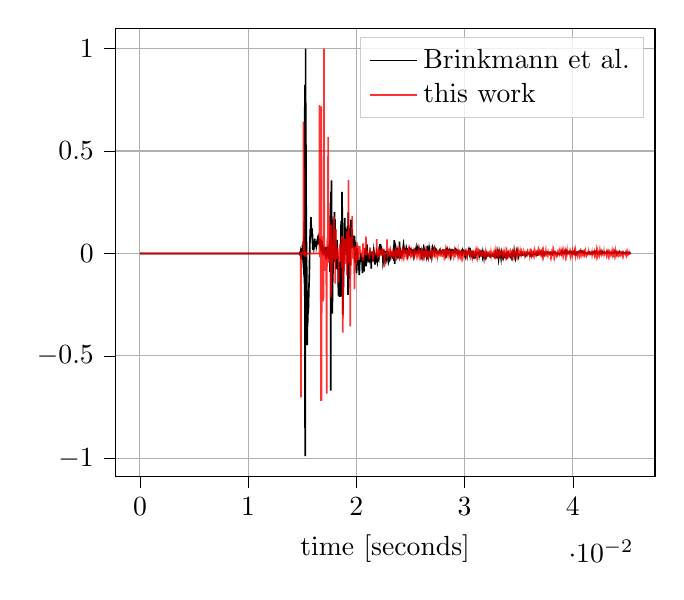
\begin{tikzpicture}

\begin{axis}[
legend cell align={left},
legend style={fill opacity=0.8, draw opacity=1, text opacity=1, draw=white!80.00000!black},
tick align=outside,
tick pos=left,
x grid style={white!69.01961!black},
xlabel={time [seconds]},
xmajorgrids,
xmin=-0.00227, xmax=0.04760,
xtick style={color=black},
y grid style={white!69.01961!black},
ymajorgrids,
ymin=-1.08905, ymax=1.09948,
ytick style={color=black}
]
\addplot [semithick, black]
table {%
0.00000 -0.00005
0.00002 -0.00001
0.00005 -0.00002
0.00007 -0.00001
0.00009 -0.00003
0.00011 -0.00004
0.00014 -0.00003
0.00016 -0.00004
0.00018 -0.00001
0.00020 -0.00001
0.00023 -0.00007
0.00025 -0.00006
0.00027 -0.00002
0.00029 -0.00002
0.00032 -0.00003
0.00034 -0.00004
0.00036 0.00000
0.00039 -0.00006
0.00041 -0.00004
0.00043 -0.00004
0.00045 0.00001
0.00048 -0.00001
0.00050 -0.00004
0.00052 -0.00004
0.00054 -0.00004
0.00057 -0.00002
0.00059 -0.00000
0.00061 -0.00001
0.00063 -0.00006
0.00066 -0.00004
0.00068 -0.00006
0.00070 -0.00001
0.00073 -0.00002
0.00075 -0.00009
0.00077 -0.00005
0.00079 -0.00004
0.00082 -0.00002
0.00084 -0.00004
0.00086 -0.00003
0.00088 -0.00006
0.00091 -0.00005
0.00093 -0.00001
0.00095 -0.00004
0.00098 -0.00004
0.00100 0.00001
0.00102 -0.00002
0.00104 -0.00005
0.00107 -0.00005
0.00109 -0.00006
0.00111 0.00000
0.00113 -0.00002
0.00116 -0.00001
0.00118 -0.00003
0.00120 -0.00004
0.00122 -0.00004
0.00125 0.00000
0.00127 -0.00002
0.00129 -0.00003
0.00132 -0.00001
0.00134 -0.00004
0.00136 -0.00005
0.00138 -0.00002
0.00141 -0.00001
0.00143 -0.00000
0.00145 -0.00002
0.00147 0.00000
0.00150 -0.00002
0.00152 -0.00002
0.00154 -0.00003
0.00156 -0.00006
0.00159 -0.00006
0.00161 -0.00002
0.00163 -0.00004
0.00166 0.00000
0.00168 -0.00002
0.00170 -0.00001
0.00172 -0.00002
0.00175 -0.00001
0.00177 -0.00002
0.00179 -0.00003
0.00181 -0.00002
0.00184 0.00000
0.00186 -0.00002
0.00188 -0.00004
0.00190 -0.00004
0.00193 -0.00000
0.00195 -0.00001
0.00197 0.00001
0.00200 -0.00003
0.00202 -0.00000
0.00204 0.00001
0.00206 -0.00002
0.00209 -0.00003
0.00211 -0.00000
0.00213 -0.00003
0.00215 -0.00005
0.00218 -0.00004
0.00220 0.00001
0.00222 -0.00005
0.00224 -0.00000
0.00227 0.00000
0.00229 -0.00003
0.00231 0.00000
0.00234 0.00003
0.00236 0.00001
0.00238 -0.00004
0.00240 -0.00001
0.00243 0.00001
0.00245 -0.00001
0.00247 -0.00002
0.00249 0.00000
0.00252 -0.00000
0.00254 0.00000
0.00256 -0.00000
0.00259 -0.00002
0.00261 -0.00002
0.00263 0.00004
0.00265 0.00003
0.00268 -0.00002
0.00270 -0.00001
0.00272 -0.00002
0.00274 -0.00002
0.00277 -0.00004
0.00279 -0.00002
0.00281 -0.00002
0.00283 0.00003
0.00286 0.00002
0.00288 0.00001
0.00290 -0.00001
0.00293 -0.00001
0.00295 -0.00002
0.00297 -0.00002
0.00299 -0.00002
0.00302 -0.00002
0.00304 -0.00003
0.00306 -0.00002
0.00308 -0.00003
0.00311 -0.00002
0.00313 0.00002
0.00315 -0.00001
0.00317 -0.00003
0.00320 -0.00003
0.00322 0.00002
0.00324 -0.00002
0.00327 -0.00002
0.00329 -0.00003
0.00331 0.00001
0.00333 -0.00004
0.00336 -0.00005
0.00338 0.00002
0.00340 -0.00001
0.00342 0.00001
0.00345 -0.00000
0.00347 -0.00004
0.00349 -0.00000
0.00351 -0.00001
0.00354 -0.00002
0.00356 -0.00003
0.00358 -0.00001
0.00361 -0.00002
0.00363 -0.00002
0.00365 -0.00002
0.00367 0.00002
0.00370 0.00002
0.00372 -0.00003
0.00374 -0.00001
0.00376 -0.00004
0.00379 -0.00001
0.00381 0.00002
0.00383 -0.00002
0.00385 0.00001
0.00388 -0.00000
0.00390 -0.00004
0.00392 -0.00005
0.00395 -0.00001
0.00397 0.00002
0.00399 0.00001
0.00401 0.00003
0.00404 -0.00003
0.00406 -0.00000
0.00408 0.00000
0.00410 -0.00004
0.00413 -0.00001
0.00415 0.00000
0.00417 -0.00003
0.00420 0.00002
0.00422 0.00001
0.00424 0.00001
0.00426 -0.00001
0.00429 0.00001
0.00431 -0.00001
0.00433 0.00001
0.00435 0.00000
0.00438 -0.00004
0.00440 0.00001
0.00442 -0.00003
0.00444 -0.00002
0.00447 -0.00000
0.00449 -0.00001
0.00451 -0.00001
0.00454 0.00002
0.00456 0.00000
0.00458 -0.00002
0.00460 0.00001
0.00463 -0.00002
0.00465 -0.00001
0.00467 0.00001
0.00469 -0.00002
0.00472 -0.00001
0.00474 0.00001
0.00476 0.00003
0.00478 -0.00000
0.00481 0.00000
0.00483 0.00003
0.00485 0.00002
0.00488 0.00001
0.00490 0.00002
0.00492 0.00001
0.00494 0.00000
0.00497 -0.00001
0.00499 0.00001
0.00501 0.00000
0.00503 0.00001
0.00506 0.00003
0.00508 0.00003
0.00510 -0.00001
0.00512 0.00002
0.00515 0.00003
0.00517 0.00002
0.00519 0.00000
0.00522 0.00000
0.00524 0.00001
0.00526 -0.00001
0.00528 -0.00001
0.00531 0.00001
0.00533 -0.00002
0.00535 -0.00001
0.00537 0.00004
0.00540 0.00003
0.00542 0.00001
0.00544 0.00004
0.00546 0.00001
0.00549 -0.00004
0.00551 0.00000
0.00553 -0.00001
0.00556 0.00001
0.00558 -0.00001
0.00560 -0.00000
0.00562 0.00002
0.00565 0.00000
0.00567 0.00005
0.00569 -0.00002
0.00571 0.00000
0.00574 0.00003
0.00576 -0.00000
0.00578 -0.00005
0.00580 0.00001
0.00583 0.00000
0.00585 -0.00004
0.00587 0.00005
0.00590 -0.00001
0.00592 -0.00001
0.00594 -0.00001
0.00596 -0.00002
0.00599 -0.00000
0.00601 -0.00000
0.00603 0.00003
0.00605 -0.00004
0.00608 -0.00006
0.00610 -0.00002
0.00612 -0.00005
0.00615 0.00000
0.00617 -0.00000
0.00619 -0.00002
0.00621 0.00002
0.00624 0.00001
0.00626 0.00001
0.00628 0.00002
0.00630 0.00001
0.00633 -0.00005
0.00635 -0.00003
0.00637 -0.00007
0.00639 -0.00002
0.00642 -0.00001
0.00644 -0.00001
0.00646 0.00003
0.00649 0.00001
0.00651 0.00000
0.00653 0.00002
0.00655 -0.00001
0.00658 -0.00001
0.00660 -0.00004
0.00662 -0.00004
0.00664 0.00000
0.00667 -0.00002
0.00669 0.00000
0.00671 0.00003
0.00673 0.00001
0.00676 -0.00001
0.00678 -0.00001
0.00680 -0.00002
0.00683 -0.00000
0.00685 -0.00003
0.00687 -0.00002
0.00689 0.00000
0.00692 -0.00001
0.00694 -0.00006
0.00696 -0.00003
0.00698 -0.00002
0.00701 -0.00001
0.00703 -0.00001
0.00705 0.00003
0.00707 -0.00001
0.00710 0.00003
0.00712 -0.00003
0.00714 0.00001
0.00717 0.00001
0.00719 -0.00001
0.00721 -0.00001
0.00723 -0.00001
0.00726 0.00003
0.00728 0.00001
0.00730 -0.00000
0.00732 0.00000
0.00735 -0.00000
0.00737 -0.00001
0.00739 0.00003
0.00741 0.00002
0.00744 -0.00001
0.00746 0.00001
0.00748 -0.00002
0.00751 -0.00003
0.00753 -0.00003
0.00755 -0.00003
0.00757 0.00001
0.00760 -0.00003
0.00762 0.00002
0.00764 0.00003
0.00766 0.00003
0.00769 -0.00000
0.00771 -0.00001
0.00773 -0.00004
0.00776 -0.00005
0.00778 -0.00000
0.00780 0.00003
0.00782 0.00000
0.00785 -0.00001
0.00787 0.00001
0.00789 0.00004
0.00791 0.00002
0.00794 0.00002
0.00796 0.00001
0.00798 -0.00001
0.00800 0.00003
0.00803 -0.00002
0.00805 0.00000
0.00807 -0.00002
0.00810 -0.00001
0.00812 -0.00000
0.00814 0.00002
0.00816 0.00000
0.00819 0.00000
0.00821 0.00003
0.00823 -0.00001
0.00825 -0.00001
0.00828 0.00001
0.00830 0.00003
0.00832 0.00002
0.00834 -0.00001
0.00837 0.00000
0.00839 -0.00003
0.00841 0.00001
0.00844 0.00002
0.00846 0.00003
0.00848 0.00003
0.00850 -0.00000
0.00853 0.00002
0.00855 0.00001
0.00857 -0.00006
0.00859 -0.00002
0.00862 -0.00004
0.00864 -0.00002
0.00866 0.00000
0.00868 0.00001
0.00871 -0.00005
0.00873 -0.00005
0.00875 0.00001
0.00878 -0.00004
0.00880 -0.00003
0.00882 -0.00000
0.00884 -0.00003
0.00887 -0.00004
0.00889 -0.00004
0.00891 -0.00003
0.00893 -0.00006
0.00896 -0.00003
0.00898 -0.00004
0.00900 -0.00000
0.00902 0.00001
0.00905 -0.00001
0.00907 -0.00004
0.00909 -0.00001
0.00912 -0.00007
0.00914 -0.00005
0.00916 -0.00003
0.00918 -0.00005
0.00921 -0.00005
0.00923 -0.00001
0.00925 -0.00002
0.00927 -0.00002
0.00930 -0.00001
0.00932 -0.00000
0.00934 -0.00001
0.00937 -0.00003
0.00939 -0.00003
0.00941 -0.00002
0.00943 -0.00002
0.00946 -0.00005
0.00948 -0.00006
0.00950 0.00002
0.00952 -0.00001
0.00955 -0.00000
0.00957 0.00002
0.00959 -0.00001
0.00961 -0.00000
0.00964 0.00003
0.00966 -0.00004
0.00968 0.00001
0.00971 -0.00003
0.00973 -0.00006
0.00975 -0.00001
0.00977 0.00000
0.00980 -0.00002
0.00982 0.00000
0.00984 -0.00001
0.00986 0.00000
0.00989 -0.00001
0.00991 -0.00003
0.00993 -0.00004
0.00995 -0.00002
0.00998 -0.00004
0.01000 -0.00001
0.01002 -0.00004
0.01005 -0.00003
0.01007 -0.00006
0.01009 -0.00006
0.01011 -0.00003
0.01014 -0.00001
0.01016 0.00000
0.01018 -0.00003
0.01020 -0.00003
0.01023 -0.00007
0.01025 -0.00008
0.01027 -0.00006
0.01029 -0.00010
0.01032 -0.00003
0.01034 -0.00004
0.01036 -0.00002
0.01039 -0.00004
0.01041 -0.00005
0.01043 -0.00005
0.01045 -0.00003
0.01048 -0.00005
0.01050 -0.00006
0.01052 -0.00009
0.01054 -0.00008
0.01057 -0.00006
0.01059 -0.00003
0.01061 -0.00003
0.01063 -0.00004
0.01066 -0.00007
0.01068 -0.00006
0.01070 0.00001
0.01073 -0.00002
0.01075 -0.00002
0.01077 -0.00003
0.01079 -0.00003
0.01082 -0.00005
0.01084 -0.00005
0.01086 -0.00003
0.01088 -0.00001
0.01091 -0.00000
0.01093 -0.00001
0.01095 -0.00003
0.01098 -0.00002
0.01100 -0.00005
0.01102 -0.00002
0.01104 -0.00005
0.01107 -0.00009
0.01109 -0.00006
0.01111 -0.00004
0.01113 -0.00004
0.01116 -0.00004
0.01118 -0.00003
0.01120 -0.00004
0.01122 -0.00006
0.01125 -0.00004
0.01127 -0.00007
0.01129 -0.00004
0.01132 -0.00004
0.01134 -0.00005
0.01136 -0.00004
0.01138 -0.00004
0.01141 -0.00008
0.01143 -0.00010
0.01145 -0.00011
0.01147 -0.00010
0.01150 -0.00008
0.01152 -0.00006
0.01154 -0.00008
0.01156 -0.00007
0.01159 -0.00014
0.01161 -0.00012
0.01163 -0.00008
0.01166 -0.00013
0.01168 -0.00010
0.01170 -0.00012
0.01172 -0.00010
0.01175 -0.00014
0.01177 -0.00011
0.01179 -0.00009
0.01181 -0.00010
0.01184 -0.00010
0.01186 -0.00007
0.01188 -0.00004
0.01190 -0.00004
0.01193 -0.00005
0.01195 -0.00012
0.01197 -0.00011
0.01200 -0.00013
0.01202 -0.00011
0.01204 -0.00007
0.01206 -0.00004
0.01209 -0.00004
0.01211 -0.00001
0.01213 0.00000
0.01215 -0.00006
0.01218 -0.00008
0.01220 -0.00004
0.01222 -0.00008
0.01224 -0.00009
0.01227 -0.00006
0.01229 -0.00006
0.01231 -0.00002
0.01234 -0.00001
0.01236 -0.00002
0.01238 -0.00006
0.01240 -0.00000
0.01243 -0.00002
0.01245 -0.00003
0.01247 -0.00002
0.01249 -0.00004
0.01252 -0.00010
0.01254 -0.00006
0.01256 -0.00011
0.01259 -0.00010
0.01261 -0.00009
0.01263 -0.00005
0.01265 -0.00007
0.01268 -0.00000
0.01270 -0.00005
0.01272 -0.00009
0.01274 -0.00014
0.01277 -0.00014
0.01279 -0.00018
0.01281 -0.00014
0.01283 -0.00013
0.01286 -0.00007
0.01288 -0.00008
0.01290 -0.00007
0.01293 -0.00011
0.01295 -0.00014
0.01297 -0.00015
0.01299 -0.00011
0.01302 -0.00015
0.01304 -0.00009
0.01306 -0.00011
0.01308 -0.00010
0.01311 -0.00015
0.01313 -0.00013
0.01315 -0.00014
0.01317 -0.00010
0.01320 -0.00016
0.01322 -0.00010
0.01324 -0.00010
0.01327 -0.00004
0.01329 -0.00013
0.01331 -0.00008
0.01333 -0.00016
0.01336 -0.00010
0.01338 -0.00011
0.01340 -0.00007
0.01342 -0.00004
0.01345 0.00000
0.01347 -0.00002
0.01349 0.00002
0.01351 -0.00008
0.01354 -0.00001
0.01356 -0.00004
0.01358 0.00002
0.01361 0.00000
0.01363 0.00005
0.01365 0.00003
0.01367 0.00005
0.01370 0.00001
0.01372 -0.00003
0.01374 -0.00006
0.01376 -0.00004
0.01379 -0.00003
0.01381 0.00000
0.01383 0.00005
0.01385 0.00002
0.01388 0.00002
0.01390 -0.00006
0.01392 -0.00008
0.01395 -0.00015
0.01397 -0.00008
0.01399 -0.00014
0.01401 -0.00007
0.01404 -0.00007
0.01406 -0.00001
0.01408 -0.00013
0.01410 -0.00006
0.01413 -0.00012
0.01415 -0.00008
0.01417 -0.00017
0.01420 -0.00010
0.01422 -0.00018
0.01424 -0.00005
0.01426 -0.00020
0.01429 -0.00011
0.01431 -0.00031
0.01433 -0.00016
0.01435 -0.00030
0.01438 -0.00011
0.01440 -0.00023
0.01442 -0.00008
0.01444 -0.00030
0.01447 -0.00019
0.01449 -0.00039
0.01451 -0.00025
0.01454 -0.00041
0.01456 -0.00018
0.01458 -0.00029
0.01460 -0.00001
0.01463 -0.00019
0.01465 0.00011
0.01467 -0.00032
0.01469 0.00017
0.01472 -0.00071
0.01474 0.00075
0.01476 -0.00142
0.01478 0.00178
0.01481 -0.00256
0.01483 0.00355
0.01485 -0.00465
0.01488 0.00636
0.01490 -0.00810
0.01492 0.01063
0.01494 -0.01338
0.01497 0.01688
0.01499 -0.02091
0.01501 0.02600
0.01503 -0.03176
0.01506 0.03901
0.01508 -0.04763
0.01510 0.05841
0.01512 -0.07213
0.01515 0.09008
0.01517 -0.11598
0.01519 0.15368
0.01522 -0.20893
0.01524 0.82272
0.01526 -0.84366
0.01528 -0.98957
0.01531 1.00000
0.01533 0.03581
0.01535 0.53148
0.01537 0.02001
0.01540 0.05794
0.01542 -0.24877
0.01544 -0.20306
0.01546 -0.44745
0.01549 -0.28925
0.01551 -0.33795
0.01553 -0.27564
0.01556 -0.28562
0.01558 -0.24839
0.01560 -0.19532
0.01562 -0.15764
0.01565 -0.11708
0.01567 -0.05244
0.01569 0.01268
0.01571 0.05664
0.01574 0.11857
0.01576 0.11179
0.01578 0.11712
0.01580 0.17770
0.01583 0.13199
0.01585 0.08729
0.01587 0.08524
0.01590 0.12186
0.01592 0.06951
0.01594 0.09607
0.01596 0.02794
0.01599 0.01731
0.01601 0.05273
0.01603 0.04630
0.01605 0.04246
0.01608 0.02606
0.01610 0.03175
0.01612 0.04432
0.01615 0.07223
0.01617 0.04840
0.01619 0.04784
0.01621 0.03291
0.01624 0.04686
0.01626 0.05222
0.01628 0.05089
0.01630 0.03710
0.01633 0.04751
0.01635 0.05388
0.01637 0.05109
0.01639 0.05657
0.01642 0.07002
0.01644 0.07902
0.01646 0.08200
0.01649 0.06863
0.01651 0.05702
0.01653 0.05921
0.01655 0.06100
0.01658 0.04862
0.01660 0.04631
0.01662 0.05049
0.01664 0.04420
0.01667 0.05100
0.01669 0.03181
0.01671 0.02570
0.01673 0.03300
0.01676 0.04360
0.01678 0.04758
0.01680 0.03981
0.01683 0.03216
0.01685 0.01698
0.01687 0.02483
0.01689 0.03785
0.01692 0.02905
0.01694 0.02174
0.01696 0.01345
0.01698 0.02039
0.01701 0.02241
0.01703 0.01167
0.01705 0.00700
0.01707 0.00819
0.01710 0.00658
0.01712 -0.00012
0.01714 0.00984
0.01717 0.00067
0.01719 0.00612
0.01721 -0.00263
0.01723 0.00706
0.01726 -0.00044
0.01728 0.02058
0.01730 -0.01606
0.01732 0.03105
0.01735 0.00188
0.01737 0.03487
0.01739 -0.00812
0.01741 0.03763
0.01744 -0.01348
0.01746 0.03789
0.01748 -0.03064
0.01751 0.04449
0.01753 -0.04603
0.01755 0.06635
0.01757 -0.08977
0.01760 0.24851
0.01762 -0.01715
0.01764 -0.67002
0.01766 0.30135
0.01769 0.10712
0.01771 0.35676
0.01773 -0.07166
0.01776 -0.22745
0.01778 -0.29349
0.01780 -0.14463
0.01782 -0.13307
0.01785 -0.05395
0.01787 -0.00755
0.01789 0.16390
0.01791 0.07344
0.01794 0.12642
0.01796 0.16079
0.01798 0.20295
0.01800 0.07366
0.01803 0.16593
0.01805 -0.04295
0.01807 -0.00594
0.01810 0.00404
0.01812 -0.07679
0.01814 0.04161
0.01816 -0.01718
0.01819 -0.07507
0.01821 0.06617
0.01823 0.03134
0.01825 -0.07359
0.01828 -0.01272
0.01830 -0.07583
0.01832 -0.07579
0.01834 -0.20644
0.01837 -0.04068
0.01839 -0.12734
0.01841 -0.09759
0.01844 -0.21246
0.01846 -0.10474
0.01848 -0.07992
0.01850 -0.18876
0.01853 -0.15553
0.01855 -0.06183
0.01857 -0.00477
0.01859 0.15818
0.01862 -0.21089
0.01864 -0.16024
0.01866 0.15751
0.01868 0.30051
0.01871 0.03945
0.01873 -0.05379
0.01875 -0.29880
0.01878 -0.20403
0.01880 -0.13224
0.01882 -0.16301
0.01884 0.04932
0.01887 -0.03186
0.01889 0.08085
0.01891 0.14622
0.01893 0.17344
0.01896 0.06172
0.01898 0.08733
0.01900 0.11976
0.01902 0.06740
0.01905 0.07938
0.01907 0.01440
0.01909 -0.00636
0.01912 0.02802
0.01914 0.00515
0.01916 -0.04753
0.01918 0.13365
0.01921 -0.00951
0.01923 -0.20170
0.01925 0.20106
0.01927 0.05226
0.01930 0.12304
0.01932 -0.04827
0.01934 0.02571
0.01937 -0.12589
0.01939 0.12033
0.01941 -0.05929
0.01943 0.07101
0.01946 0.00773
0.01948 0.11884
0.01950 0.16496
0.01952 0.07136
0.01955 0.04803
0.01957 0.09774
0.01959 0.11866
0.01961 0.02662
0.01964 0.08656
0.01966 0.06290
0.01968 0.05081
0.01971 0.04370
0.01973 0.08735
0.01975 0.07770
0.01977 0.04106
0.01980 0.05545
0.01982 0.04646
0.01984 0.08441
0.01986 -0.02587
0.01989 -0.02086
0.01991 0.05519
0.01993 0.04787
0.01995 -0.01058
0.01998 -0.05645
0.02000 -0.08897
0.02002 -0.09705
0.02005 -0.05069
0.02007 -0.00545
0.02009 0.02574
0.02011 0.00930
0.02014 -0.03633
0.02016 -0.03752
0.02018 -0.05297
0.02020 -0.03294
0.02023 -0.05923
0.02025 -0.08166
0.02027 -0.10570
0.02029 -0.07477
0.02032 -0.03674
0.02034 -0.03715
0.02036 -0.02381
0.02039 -0.01629
0.02041 0.00004
0.02043 -0.00824
0.02045 -0.01462
0.02048 -0.03044
0.02050 -0.03521
0.02052 -0.01767
0.02054 -0.06725
0.02057 -0.09602
0.02059 -0.06419
0.02061 -0.02299
0.02063 -0.04040
0.02066 -0.05033
0.02068 -0.08190
0.02070 -0.08272
0.02073 -0.04431
0.02075 -0.01000
0.02077 -0.01959
0.02079 0.00279
0.02082 0.02532
0.02084 -0.00198
0.02086 -0.02348
0.02088 -0.06293
0.02091 -0.05144
0.02093 -0.01221
0.02095 0.01552
0.02098 0.04440
0.02100 0.01532
0.02102 -0.00382
0.02104 -0.00576
0.02107 -0.00890
0.02109 -0.02165
0.02111 -0.03909
0.02113 -0.03846
0.02116 -0.02909
0.02118 -0.01346
0.02120 -0.01089
0.02122 -0.01818
0.02125 0.00311
0.02127 0.00922
0.02129 0.00613
0.02132 0.00196
0.02134 -0.00324
0.02136 -0.02129
0.02138 -0.07341
0.02141 0.00844
0.02143 0.00191
0.02145 0.00884
0.02147 -0.02796
0.02150 -0.02994
0.02152 -0.02232
0.02154 -0.03755
0.02156 -0.00446
0.02159 0.00162
0.02161 0.01371
0.02163 0.00486
0.02166 -0.01091
0.02168 -0.03706
0.02170 -0.03610
0.02172 -0.05392
0.02175 -0.03553
0.02177 -0.03650
0.02179 -0.03093
0.02181 -0.03247
0.02184 -0.00583
0.02186 0.00073
0.02188 -0.00906
0.02190 -0.02956
0.02193 -0.03783
0.02195 -0.02171
0.02197 -0.01724
0.02200 -0.02325
0.02202 -0.02395
0.02204 -0.03065
0.02206 -0.03231
0.02209 -0.01398
0.02211 0.00863
0.02213 0.02559
0.02215 0.03614
0.02218 0.04657
0.02220 0.01953
0.02222 -0.00580
0.02224 0.01943
0.02227 0.02229
0.02229 0.01409
0.02231 0.01953
0.02234 0.00702
0.02236 -0.00093
0.02238 0.01643
0.02240 0.01630
0.02243 -0.00536
0.02245 -0.02421
0.02247 -0.04578
0.02249 -0.03939
0.02252 -0.00150
0.02254 0.02016
0.02256 -0.00684
0.02259 -0.02279
0.02261 -0.02814
0.02263 -0.02168
0.02265 -0.02693
0.02268 -0.00496
0.02270 -0.00181
0.02272 0.01140
0.02274 -0.00610
0.02277 -0.01724
0.02279 -0.00697
0.02281 -0.00757
0.02283 0.01478
0.02286 -0.00326
0.02288 -0.01216
0.02290 -0.01955
0.02293 -0.00845
0.02295 -0.00644
0.02297 -0.00364
0.02299 -0.03849
0.02302 -0.03315
0.02304 -0.03386
0.02306 -0.02841
0.02308 -0.01824
0.02311 -0.02200
0.02313 -0.01441
0.02315 -0.01459
0.02317 -0.00461
0.02320 -0.01324
0.02322 -0.01196
0.02324 0.00194
0.02327 0.00153
0.02329 -0.00724
0.02331 -0.01234
0.02333 -0.01858
0.02336 -0.01613
0.02338 -0.01365
0.02340 -0.00120
0.02342 -0.00925
0.02345 -0.01150
0.02347 -0.03560
0.02349 0.06488
0.02351 0.02699
0.02354 -0.05026
0.02356 -0.01346
0.02358 -0.01197
0.02361 0.03410
0.02363 0.02877
0.02365 0.01947
0.02367 0.01140
0.02370 0.01420
0.02372 0.00032
0.02374 -0.00762
0.02376 -0.01782
0.02379 -0.01235
0.02381 -0.01296
0.02383 -0.00159
0.02385 -0.01087
0.02388 -0.01139
0.02390 -0.01404
0.02392 0.02156
0.02395 -0.01610
0.02397 -0.00038
0.02399 0.05807
0.02401 -0.01654
0.02404 0.01923
0.02406 -0.01665
0.02408 -0.00931
0.02410 -0.02458
0.02413 -0.00576
0.02415 -0.00578
0.02417 0.00461
0.02420 0.00238
0.02422 -0.00991
0.02424 -0.01015
0.02426 0.00217
0.02429 0.01326
0.02431 0.02386
0.02433 0.03171
0.02435 0.02004
0.02438 0.03539
0.02440 0.02666
0.02442 0.01299
0.02444 0.01493
0.02447 0.00516
0.02449 0.00436
0.02451 0.00981
0.02454 0.01476
0.02456 -0.00163
0.02458 0.00881
0.02460 0.01500
0.02463 0.02632
0.02465 0.02227
0.02467 0.00943
0.02469 0.00413
0.02472 -0.00532
0.02474 0.00036
0.02476 -0.00800
0.02478 -0.00188
0.02481 0.00405
0.02483 0.00527
0.02485 0.00923
0.02488 0.01385
0.02490 0.00879
0.02492 0.01813
0.02494 0.01446
0.02497 0.02089
0.02499 0.01955
0.02501 0.01694
0.02503 0.01308
0.02506 0.00737
0.02508 0.01464
0.02510 0.01147
0.02512 0.01527
0.02515 0.01345
0.02517 0.01374
0.02519 0.00950
0.02522 0.00350
0.02524 -0.00265
0.02526 0.01628
0.02528 0.01659
0.02531 0.00330
0.02533 0.00331
0.02535 -0.00259
0.02537 0.00901
0.02540 0.00402
0.02542 0.01024
0.02544 0.01192
0.02546 0.01698
0.02549 0.01869
0.02551 0.02391
0.02553 0.00551
0.02556 0.00424
0.02558 0.01203
0.02560 0.01126
0.02562 0.02000
0.02565 0.02639
0.02567 0.02191
0.02569 0.01794
0.02571 0.01599
0.02574 0.00670
0.02576 0.00984
0.02578 0.00845
0.02580 0.01979
0.02583 0.01176
0.02585 0.01403
0.02587 0.01382
0.02590 0.01586
0.02592 0.02571
0.02594 0.01291
0.02596 0.01032
0.02599 -0.00432
0.02601 0.00208
0.02603 0.01100
0.02605 0.00766
0.02608 -0.00577
0.02610 0.00337
0.02612 0.00733
0.02615 0.01470
0.02617 0.01876
0.02619 -0.01078
0.02621 0.00546
0.02624 -0.00489
0.02626 0.00802
0.02628 -0.00943
0.02630 0.01249
0.02633 0.00480
0.02635 0.01659
0.02637 0.00613
0.02639 0.00818
0.02642 -0.00835
0.02644 0.00651
0.02646 0.00461
0.02649 0.01726
0.02651 -0.00860
0.02653 -0.00361
0.02655 0.03690
0.02658 -0.02859
0.02660 0.01546
0.02662 -0.01308
0.02664 0.00538
0.02667 -0.00509
0.02669 0.00807
0.02671 0.00545
0.02673 0.01894
0.02676 0.00606
0.02678 0.01116
0.02680 -0.00071
0.02683 -0.00287
0.02685 -0.00913
0.02687 -0.00415
0.02689 -0.00444
0.02692 -0.00336
0.02694 -0.00785
0.02696 0.00082
0.02698 -0.01041
0.02701 0.00193
0.02703 0.01843
0.02705 0.03018
0.02707 0.02734
0.02710 0.01607
0.02712 0.00932
0.02714 0.01004
0.02717 0.01563
0.02719 0.01712
0.02721 0.02765
0.02723 0.01465
0.02726 0.02557
0.02728 0.02277
0.02730 0.00294
0.02732 0.02594
0.02735 0.01295
0.02737 0.01130
0.02739 0.00815
0.02741 0.00097
0.02744 0.00014
0.02746 0.00564
0.02748 0.00178
0.02751 0.00429
0.02753 0.00885
0.02755 0.00873
0.02757 0.00649
0.02760 0.00454
0.02762 0.00301
0.02764 0.00688
0.02766 0.01213
0.02769 0.01641
0.02771 0.01543
0.02773 0.01700
0.02776 0.01131
0.02778 0.00857
0.02780 0.00298
0.02782 0.00110
0.02785 0.00456
0.02787 0.00768
0.02789 0.00852
0.02791 0.01020
0.02794 0.01263
0.02796 0.00753
0.02798 0.00814
0.02800 0.01339
0.02803 0.01148
0.02805 0.01282
0.02807 -0.00088
0.02810 0.00035
0.02812 -0.00185
0.02814 -0.00128
0.02816 0.00090
0.02819 -0.00563
0.02821 -0.00867
0.02823 -0.00125
0.02825 -0.00730
0.02828 -0.00976
0.02830 0.00911
0.02832 0.00339
0.02834 0.01187
0.02837 0.01631
0.02839 0.00482
0.02841 0.00993
0.02844 0.00782
0.02846 0.01413
0.02848 0.01172
0.02850 0.01329
0.02853 0.00698
0.02855 0.01015
0.02857 0.00580
0.02859 0.00666
0.02862 0.01104
0.02864 0.00866
0.02866 0.00178
0.02868 0.01170
0.02871 0.00688
0.02873 0.00888
0.02875 -0.00513
0.02878 0.00426
0.02880 0.00599
0.02882 0.00899
0.02884 0.00502
0.02887 0.00599
0.02889 0.01041
0.02891 0.00736
0.02893 0.01398
0.02896 0.01501
0.02898 0.00930
0.02900 0.01096
0.02902 0.00877
0.02905 0.00778
0.02907 0.00658
0.02909 0.00632
0.02912 0.00725
0.02914 0.01176
0.02916 0.00583
0.02918 0.00765
0.02921 0.01257
0.02923 0.00801
0.02925 0.00693
0.02927 0.00574
0.02930 0.00925
0.02932 0.01230
0.02934 0.01021
0.02937 0.00654
0.02939 -0.00004
0.02941 0.00477
0.02943 0.00752
0.02946 0.01018
0.02948 0.00611
0.02950 0.00720
0.02952 0.00261
0.02955 0.00666
0.02957 0.00733
0.02959 0.00390
0.02961 0.00373
0.02964 0.00217
0.02966 0.00249
0.02968 -0.00128
0.02971 0.00486
0.02973 0.00105
0.02975 0.00513
0.02977 0.00857
0.02980 0.00411
0.02982 0.01204
0.02984 0.00827
0.02986 0.01101
0.02989 0.00644
0.02991 0.00761
0.02993 0.00622
0.02995 0.00938
0.02998 0.00602
0.03000 0.00308
0.03002 -0.00554
0.03005 -0.00177
0.03007 -0.00740
0.03009 0.00299
0.03011 -0.00074
0.03014 0.00062
0.03016 0.00347
0.03018 0.00558
0.03020 0.00459
0.03023 0.00300
0.03025 -0.00755
0.03027 -0.00122
0.03029 0.00213
0.03032 0.00522
0.03034 0.01061
0.03036 0.00449
0.03039 0.00191
0.03041 0.00193
0.03043 0.00774
0.03045 0.00240
0.03048 0.00975
0.03050 0.00152
0.03052 0.01423
0.03054 0.01607
0.03057 0.00970
0.03059 0.00205
0.03061 -0.00047
0.03063 -0.00564
0.03066 -0.00998
0.03068 -0.00471
0.03070 -0.00862
0.03073 -0.00178
0.03075 -0.00576
0.03077 -0.00981
0.03079 -0.00273
0.03082 -0.01003
0.03084 -0.00578
0.03086 -0.01206
0.03088 -0.01656
0.03091 -0.02016
0.03093 -0.02162
0.03095 -0.02196
0.03098 -0.01975
0.03100 -0.01182
0.03102 -0.00419
0.03104 -0.00992
0.03107 -0.00946
0.03109 -0.00729
0.03111 -0.00018
0.03113 0.00464
0.03116 0.00542
0.03118 0.00631
0.03120 0.00437
0.03122 0.00076
0.03125 0.00174
0.03127 -0.00023
0.03129 -0.00197
0.03132 0.00064
0.03134 -0.00702
0.03136 0.00092
0.03138 0.00139
0.03141 0.00137
0.03143 0.00709
0.03145 0.00376
0.03147 -0.00649
0.03150 -0.00361
0.03152 0.00044
0.03154 -0.00196
0.03156 0.00321
0.03159 -0.00128
0.03161 -0.00890
0.03163 -0.00797
0.03166 0.00146
0.03168 -0.01198
0.03170 -0.00649
0.03172 0.00692
0.03175 0.00649
0.03177 -0.00275
0.03179 -0.01042
0.03181 0.00518
0.03184 0.00329
0.03186 -0.01305
0.03188 -0.01064
0.03190 -0.01007
0.03193 -0.01711
0.03195 -0.01869
0.03197 -0.02275
0.03200 -0.01771
0.03202 -0.01033
0.03204 -0.00339
0.03206 -0.00701
0.03209 -0.00269
0.03211 -0.00523
0.03213 -0.00171
0.03215 -0.00057
0.03218 -0.00009
0.03220 -0.00441
0.03222 -0.00778
0.03224 -0.00980
0.03227 -0.01034
0.03229 -0.00994
0.03231 -0.01270
0.03234 -0.01372
0.03236 -0.01491
0.03238 -0.00916
0.03240 -0.00609
0.03243 -0.00811
0.03245 -0.01005
0.03247 -0.00867
0.03249 -0.00909
0.03252 -0.00897
0.03254 -0.00971
0.03256 -0.01073
0.03259 -0.00919
0.03261 -0.00702
0.03263 -0.00857
0.03265 -0.00754
0.03268 -0.00827
0.03270 -0.01194
0.03272 -0.01352
0.03274 -0.00800
0.03277 -0.00966
0.03279 -0.00951
0.03281 -0.00377
0.03283 -0.00927
0.03286 -0.01618
0.03288 -0.02422
0.03290 0.00491
0.03293 0.00226
0.03295 -0.01913
0.03297 -0.00240
0.03299 -0.00117
0.03302 -0.01615
0.03304 -0.01521
0.03306 -0.00294
0.03308 -0.01082
0.03311 -0.01642
0.03313 -0.02433
0.03315 -0.01148
0.03317 -0.01819
0.03320 -0.01614
0.03322 0.00275
0.03324 -0.00327
0.03327 0.00435
0.03329 0.00371
0.03331 0.00470
0.03333 -0.00857
0.03336 -0.01879
0.03338 0.00139
0.03340 0.00901
0.03342 0.00473
0.03345 0.00607
0.03347 0.00094
0.03349 -0.01392
0.03351 -0.01936
0.03354 -0.02232
0.03356 -0.02562
0.03358 -0.02168
0.03361 -0.01738
0.03363 -0.00943
0.03365 -0.00272
0.03367 -0.00916
0.03370 -0.01017
0.03372 -0.01716
0.03374 -0.01817
0.03376 -0.01577
0.03379 -0.00980
0.03381 -0.00735
0.03383 -0.01494
0.03385 -0.01746
0.03388 -0.00845
0.03390 -0.00441
0.03392 -0.01214
0.03395 -0.01485
0.03397 -0.01633
0.03399 -0.00551
0.03401 -0.00141
0.03404 -0.00441
0.03406 -0.00056
0.03408 -0.00502
0.03410 -0.00586
0.03413 -0.00821
0.03415 -0.00738
0.03417 -0.01398
0.03420 -0.01416
0.03422 -0.01544
0.03424 -0.01283
0.03426 -0.01434
0.03429 -0.01855
0.03431 0.00013
0.03433 0.00190
0.03435 0.00020
0.03438 -0.00329
0.03440 -0.01001
0.03442 -0.01505
0.03444 -0.01906
0.03447 0.00015
0.03449 -0.00395
0.03451 -0.00901
0.03454 -0.00788
0.03456 -0.00660
0.03458 0.00641
0.03460 -0.00179
0.03463 -0.00632
0.03465 -0.01467
0.03467 -0.02252
0.03469 -0.02667
0.03472 -0.01853
0.03474 -0.01027
0.03476 -0.00174
0.03478 0.00371
0.03481 0.00277
0.03483 0.01067
0.03485 0.01765
0.03488 0.01421
0.03490 0.00216
0.03492 -0.00102
0.03494 -0.00156
0.03497 -0.01265
0.03499 -0.01637
0.03501 -0.01049
0.03503 -0.00788
0.03506 -0.00506
0.03508 -0.00519
0.03510 -0.00671
0.03512 -0.00660
0.03515 -0.00710
0.03517 -0.00547
0.03519 0.00239
0.03522 0.00080
0.03524 -0.00554
0.03526 -0.00815
0.03528 -0.00692
0.03531 0.00034
0.03533 -0.00335
0.03535 -0.00246
0.03537 -0.00661
0.03540 -0.00795
0.03542 -0.00646
0.03544 -0.00312
0.03546 -0.00228
0.03549 -0.00359
0.03551 -0.00176
0.03553 0.00035
0.03556 -0.00037
0.03558 -0.00270
0.03560 -0.00872
0.03562 -0.00776
0.03565 -0.00523
0.03567 -0.01044
0.03569 -0.00822
0.03571 -0.00254
0.03574 -0.00112
0.03576 -0.00304
0.03578 0.00064
0.03580 -0.00353
0.03583 -0.00221
0.03585 -0.00112
0.03587 -0.00179
0.03590 0.00054
0.03592 0.00230
0.03594 0.00151
0.03596 0.00056
0.03599 0.00059
0.03601 -0.00159
0.03603 -0.00572
0.03605 -0.00374
0.03608 -0.00536
0.03610 -0.01011
0.03612 -0.01119
0.03615 -0.00267
0.03617 -0.00965
0.03619 -0.00903
0.03621 -0.00804
0.03624 -0.00997
0.03626 -0.00873
0.03628 -0.00740
0.03630 -0.00685
0.03633 -0.00590
0.03635 -0.00101
0.03637 -0.00485
0.03639 -0.00459
0.03642 -0.00125
0.03644 -0.00139
0.03646 -0.00344
0.03649 -0.00426
0.03651 0.00012
0.03653 0.00076
0.03655 -0.00039
0.03658 -0.00146
0.03660 0.00039
0.03662 -0.00071
0.03664 0.00032
0.03667 -0.00101
0.03669 -0.00779
0.03671 -0.00671
0.03673 0.00139
0.03676 -0.00307
0.03678 -0.00090
0.03680 0.00330
0.03683 0.00025
0.03685 -0.00002
0.03687 0.00042
0.03689 -0.00288
0.03692 -0.00428
0.03694 -0.00375
0.03696 -0.00180
0.03698 0.00464
0.03701 0.00704
0.03703 0.01037
0.03705 0.01150
0.03707 0.00755
0.03710 0.00207
0.03712 0.00073
0.03714 -0.00394
0.03717 -0.00703
0.03719 -0.00932
0.03721 -0.00434
0.03723 -0.00028
0.03726 0.00486
0.03728 0.00701
0.03730 0.00356
0.03732 -0.00056
0.03735 -0.00433
0.03737 -0.00079
0.03739 -0.00480
0.03741 -0.00425
0.03744 -0.00005
0.03746 -0.00144
0.03748 -0.00153
0.03751 -0.00059
0.03753 0.00039
0.03755 -0.00079
0.03757 -0.00070
0.03760 0.00361
0.03762 0.00670
0.03764 0.00587
0.03766 0.00452
0.03769 0.00092
0.03771 0.00124
0.03773 0.00260
0.03776 0.00189
0.03778 0.00134
0.03780 0.00296
0.03782 0.00041
0.03785 -0.00047
0.03787 -0.00264
0.03789 -0.00389
0.03791 -0.00258
0.03794 0.00241
0.03796 0.00394
0.03798 0.00490
0.03800 0.00406
0.03803 0.00189
0.03805 -0.00224
0.03807 -0.00169
0.03810 0.00191
0.03812 0.00147
0.03814 0.00314
0.03816 -0.00213
0.03819 0.00063
0.03821 0.00313
0.03823 0.00513
0.03825 0.00474
0.03828 0.00633
0.03830 0.00700
0.03832 0.00515
0.03834 0.00156
0.03837 0.00250
0.03839 0.00315
0.03841 0.00395
0.03844 -0.00031
0.03846 -0.00055
0.03848 0.00078
0.03850 0.00073
0.03853 -0.00154
0.03855 0.00124
0.03857 0.00167
0.03859 0.00009
0.03862 -0.00291
0.03864 -0.00187
0.03866 -0.00100
0.03868 0.00031
0.03871 -0.00047
0.03873 -0.00151
0.03875 -0.00229
0.03878 -0.00248
0.03880 -0.00255
0.03882 -0.00044
0.03884 0.00173
0.03887 0.00207
0.03889 0.00352
0.03891 0.00288
0.03893 0.00474
0.03896 0.00850
0.03898 0.00604
0.03900 0.00004
0.03902 0.00215
0.03905 0.00542
0.03907 0.00239
0.03909 0.00354
0.03912 0.00466
0.03914 0.00297
0.03916 0.00210
0.03918 0.00505
0.03921 0.00445
0.03923 0.00327
0.03925 0.00675
0.03927 0.00169
0.03930 0.00214
0.03932 0.00107
0.03934 0.00547
0.03937 0.00636
0.03939 0.01021
0.03941 0.00665
0.03943 0.00299
0.03946 0.00640
0.03948 0.00885
0.03950 0.00707
0.03952 0.00676
0.03955 0.00386
0.03957 0.00547
0.03959 0.00519
0.03961 0.00378
0.03964 0.00634
0.03966 0.00457
0.03968 0.00526
0.03971 0.00420
0.03973 0.00389
0.03975 0.00612
0.03977 0.00459
0.03980 0.00299
0.03982 0.00677
0.03984 0.00506
0.03986 0.00832
0.03989 0.00866
0.03991 0.00367
0.03993 0.00161
0.03995 0.00320
0.03998 -0.00012
0.04000 0.00119
0.04002 0.00088
0.04005 -0.00048
0.04007 0.00030
0.04009 0.00388
0.04011 0.00122
0.04014 0.00569
0.04016 0.00979
0.04018 0.00715
0.04020 0.00575
0.04023 0.00052
0.04025 0.00384
0.04027 0.00537
0.04029 0.00568
0.04032 0.00110
0.04034 0.00532
0.04036 0.00558
0.04039 0.00339
0.04041 0.00009
0.04043 -0.00077
0.04045 0.00286
0.04048 0.00374
0.04050 0.00664
0.04052 0.00596
0.04054 0.00624
0.04057 0.00958
0.04059 0.00938
0.04061 0.00705
0.04063 0.00753
0.04066 0.01005
0.04068 0.00846
0.04070 0.00991
0.04073 0.00621
0.04075 0.00735
0.04077 0.01088
0.04079 0.00907
0.04082 0.00583
0.04084 0.00656
0.04086 0.00957
0.04088 0.00916
0.04091 0.00787
0.04093 0.00616
0.04095 0.00890
0.04098 0.00661
0.04100 0.00405
0.04102 0.00514
0.04104 0.00550
0.04107 0.00234
0.04109 0.00575
0.04111 0.00453
0.04113 0.00349
0.04116 0.00430
0.04118 0.00425
0.04120 0.00375
0.04122 0.00204
0.04125 0.00047
0.04127 0.00022
0.04129 0.00015
0.04132 -0.00095
0.04134 0.00161
0.04136 0.00201
0.04138 0.00154
0.04141 0.00181
0.04143 0.00366
0.04145 0.00404
0.04147 0.00373
0.04150 0.00105
0.04152 0.00231
0.04154 0.00276
0.04156 0.00488
0.04159 0.00173
0.04161 0.00063
0.04163 0.00409
0.04166 0.00348
0.04168 0.00365
0.04170 0.00199
0.04172 0.00175
0.04175 0.00032
0.04177 -0.00091
0.04179 0.00074
0.04181 0.00317
0.04184 0.00542
0.04186 0.00441
0.04188 0.00371
0.04190 0.00221
0.04193 0.00505
0.04195 0.00714
0.04197 0.00624
0.04200 0.00619
0.04202 0.00420
0.04204 0.00723
0.04206 0.00502
0.04209 0.00312
0.04211 0.00466
0.04213 0.00021
0.04215 0.00104
0.04218 0.00580
0.04220 0.00215
0.04222 0.00245
0.04224 0.00309
0.04227 0.00431
0.04229 0.00287
0.04231 -0.00079
0.04234 0.00103
0.04236 0.00263
0.04238 0.00421
0.04240 0.00419
0.04243 0.00283
0.04245 0.00127
0.04247 0.00420
0.04249 0.00636
0.04252 0.00862
0.04254 0.00509
0.04256 0.00241
0.04259 0.00674
0.04261 0.00692
0.04263 0.00338
0.04265 0.00196
0.04268 0.00471
0.04270 0.00817
0.04272 0.00476
0.04274 0.00295
0.04277 0.00472
0.04279 0.00261
0.04281 0.00239
0.04283 0.00348
0.04286 0.00224
0.04288 0.00234
0.04290 0.00488
0.04293 0.00612
0.04295 0.00491
0.04297 0.00373
0.04299 0.00316
0.04302 0.00323
0.04304 0.00363
0.04306 0.00312
0.04308 0.00400
0.04311 0.00151
0.04313 0.00246
0.04315 0.00685
0.04317 0.00888
0.04320 0.00633
0.04322 0.00550
0.04324 0.00285
0.04327 0.00257
0.04329 0.00328
0.04331 0.00339
0.04333 0.00522
0.04336 0.00432
0.04338 0.00424
0.04340 0.00491
0.04342 0.00331
0.04345 0.00254
0.04347 0.00398
0.04349 0.00402
0.04351 0.00452
0.04354 0.00370
0.04356 0.00573
0.04358 0.00602
0.04361 0.00400
0.04363 0.00019
0.04365 0.00155
0.04367 0.00211
0.04370 0.00476
0.04372 0.00496
0.04374 0.00531
0.04376 0.00320
0.04379 0.00060
0.04381 0.00098
0.04383 0.00395
0.04385 0.00768
0.04388 0.01079
0.04390 0.00868
0.04392 0.00545
0.04395 0.00551
0.04397 0.00662
0.04399 0.00581
0.04401 0.00599
0.04404 0.00410
0.04406 -0.00103
0.04408 0.00139
0.04410 0.00050
0.04413 0.00218
0.04415 0.00590
0.04417 0.00620
0.04420 0.00418
0.04422 0.00358
0.04424 0.00227
0.04426 0.00284
0.04429 0.00231
0.04431 0.00322
0.04433 0.00623
0.04435 0.00317
0.04438 0.00167
0.04440 0.00299
0.04442 0.00428
0.04444 0.00363
0.04447 0.00311
0.04449 0.00400
0.04451 0.00461
0.04454 0.00248
0.04456 0.00133
0.04458 0.00240
0.04460 0.00067
0.04463 0.00242
0.04465 0.00363
0.04467 0.00126
0.04469 0.00253
0.04472 0.00339
0.04474 0.00324
0.04476 0.00146
0.04478 0.00055
0.04481 0.00199
0.04483 0.00266
0.04485 0.00256
0.04488 0.00267
0.04490 0.00196
0.04492 0.00030
0.04494 0.00152
0.04497 0.00454
0.04499 0.00496
0.04501 0.00446
0.04503 0.00424
0.04506 0.00389
0.04508 0.00429
0.04510 0.00510
0.04512 0.00464
0.04515 0.00199
0.04517 0.00382
0.04519 0.00324
0.04522 0.00208
0.04524 0.00288
0.04526 0.00253
0.04528 0.00220
0.04531 0.00160
0.04533 0.00301
};
\addlegendentry{Brinkmann et al.}
\addplot [semithick, red, opacity=0.8]
table {%
0.00000 0.00000
0.00002 0.00000
0.00005 0.00000
0.00007 0.00000
0.00009 0.00000
0.00011 0.00000
0.00014 0.00000
0.00016 0.00000
0.00018 0.00000
0.00020 0.00000
0.00023 0.00000
0.00025 0.00000
0.00027 0.00000
0.00029 0.00000
0.00032 0.00000
0.00034 0.00000
0.00036 0.00000
0.00039 0.00000
0.00041 0.00000
0.00043 0.00000
0.00045 0.00000
0.00048 0.00000
0.00050 0.00000
0.00052 0.00000
0.00054 0.00000
0.00057 0.00000
0.00059 0.00000
0.00061 0.00000
0.00063 0.00000
0.00066 0.00000
0.00068 0.00000
0.00070 0.00000
0.00073 0.00000
0.00075 0.00000
0.00077 0.00000
0.00079 0.00000
0.00082 0.00000
0.00084 0.00000
0.00086 0.00000
0.00088 0.00000
0.00091 0.00000
0.00093 0.00000
0.00095 0.00000
0.00098 0.00000
0.00100 0.00000
0.00102 0.00000
0.00104 0.00000
0.00107 0.00000
0.00109 0.00000
0.00111 0.00000
0.00113 0.00000
0.00116 0.00000
0.00118 0.00000
0.00120 0.00000
0.00122 0.00000
0.00125 0.00000
0.00127 0.00000
0.00129 0.00000
0.00132 0.00000
0.00134 0.00000
0.00136 0.00000
0.00138 0.00000
0.00141 0.00000
0.00143 0.00000
0.00145 0.00000
0.00147 0.00000
0.00150 0.00000
0.00152 0.00000
0.00154 0.00000
0.00156 0.00000
0.00159 0.00000
0.00161 0.00000
0.00163 0.00000
0.00166 0.00000
0.00168 0.00000
0.00170 0.00000
0.00172 0.00000
0.00175 0.00000
0.00177 0.00000
0.00179 0.00000
0.00181 0.00000
0.00184 0.00000
0.00186 0.00000
0.00188 0.00000
0.00190 0.00000
0.00193 0.00000
0.00195 0.00000
0.00197 0.00000
0.00200 0.00000
0.00202 0.00000
0.00204 0.00000
0.00206 0.00000
0.00209 0.00000
0.00211 0.00000
0.00213 0.00000
0.00215 0.00000
0.00218 0.00000
0.00220 0.00000
0.00222 0.00000
0.00224 0.00000
0.00227 0.00000
0.00229 0.00000
0.00231 0.00000
0.00234 0.00000
0.00236 0.00000
0.00238 0.00000
0.00240 0.00000
0.00243 0.00000
0.00245 0.00000
0.00247 0.00000
0.00249 0.00000
0.00252 0.00000
0.00254 0.00000
0.00256 0.00000
0.00259 0.00000
0.00261 0.00000
0.00263 0.00000
0.00265 0.00000
0.00268 0.00000
0.00270 0.00000
0.00272 0.00000
0.00274 0.00000
0.00277 0.00000
0.00279 0.00000
0.00281 0.00000
0.00283 0.00000
0.00286 0.00000
0.00288 0.00000
0.00290 0.00000
0.00293 0.00000
0.00295 0.00000
0.00297 0.00000
0.00299 0.00000
0.00302 0.00000
0.00304 0.00000
0.00306 0.00000
0.00308 0.00000
0.00311 0.00000
0.00313 0.00000
0.00315 0.00000
0.00317 0.00000
0.00320 0.00000
0.00322 0.00000
0.00324 0.00000
0.00327 0.00000
0.00329 0.00000
0.00331 0.00000
0.00333 0.00000
0.00336 0.00000
0.00338 0.00000
0.00340 0.00000
0.00342 0.00000
0.00345 0.00000
0.00347 0.00000
0.00349 0.00000
0.00351 0.00000
0.00354 0.00000
0.00356 0.00000
0.00358 0.00000
0.00361 0.00000
0.00363 0.00000
0.00365 0.00000
0.00367 0.00000
0.00370 0.00000
0.00372 0.00000
0.00374 0.00000
0.00376 0.00000
0.00379 0.00000
0.00381 0.00000
0.00383 0.00000
0.00385 0.00000
0.00388 0.00000
0.00390 0.00000
0.00392 0.00000
0.00395 0.00000
0.00397 0.00000
0.00399 0.00000
0.00401 0.00000
0.00404 0.00000
0.00406 0.00000
0.00408 0.00000
0.00410 0.00000
0.00413 0.00000
0.00415 0.00000
0.00417 0.00000
0.00420 0.00000
0.00422 0.00000
0.00424 0.00000
0.00426 0.00000
0.00429 0.00000
0.00431 0.00000
0.00433 0.00000
0.00435 0.00000
0.00438 0.00000
0.00440 0.00000
0.00442 0.00000
0.00444 0.00000
0.00447 0.00000
0.00449 0.00000
0.00451 0.00000
0.00454 0.00000
0.00456 0.00000
0.00458 0.00000
0.00460 0.00000
0.00463 0.00000
0.00465 0.00000
0.00467 0.00000
0.00469 0.00000
0.00472 0.00000
0.00474 0.00000
0.00476 0.00000
0.00478 0.00000
0.00481 0.00000
0.00483 0.00000
0.00485 0.00000
0.00488 0.00000
0.00490 0.00000
0.00492 0.00000
0.00494 0.00000
0.00497 0.00000
0.00499 0.00000
0.00501 0.00000
0.00503 0.00000
0.00506 0.00000
0.00508 0.00000
0.00510 0.00000
0.00512 0.00000
0.00515 0.00000
0.00517 0.00000
0.00519 0.00000
0.00522 0.00000
0.00524 0.00000
0.00526 0.00000
0.00528 0.00000
0.00531 0.00000
0.00533 0.00000
0.00535 0.00000
0.00537 0.00000
0.00540 0.00000
0.00542 0.00000
0.00544 0.00000
0.00546 0.00000
0.00549 0.00000
0.00551 0.00000
0.00553 0.00000
0.00556 0.00000
0.00558 0.00000
0.00560 0.00000
0.00562 0.00000
0.00565 0.00000
0.00567 0.00000
0.00569 0.00000
0.00571 0.00000
0.00574 0.00000
0.00576 0.00000
0.00578 0.00000
0.00580 0.00000
0.00583 0.00000
0.00585 0.00000
0.00587 0.00000
0.00590 0.00000
0.00592 0.00000
0.00594 0.00000
0.00596 0.00000
0.00599 0.00000
0.00601 0.00000
0.00603 0.00000
0.00605 0.00000
0.00608 0.00000
0.00610 0.00000
0.00612 0.00000
0.00615 0.00000
0.00617 0.00000
0.00619 0.00000
0.00621 0.00000
0.00624 0.00000
0.00626 0.00000
0.00628 0.00000
0.00630 0.00000
0.00633 0.00000
0.00635 0.00000
0.00637 0.00000
0.00639 0.00000
0.00642 0.00000
0.00644 0.00000
0.00646 0.00000
0.00649 0.00000
0.00651 0.00000
0.00653 0.00000
0.00655 0.00000
0.00658 0.00000
0.00660 0.00000
0.00662 0.00000
0.00664 0.00000
0.00667 0.00000
0.00669 0.00000
0.00671 0.00000
0.00673 0.00000
0.00676 0.00000
0.00678 0.00000
0.00680 0.00000
0.00683 0.00000
0.00685 0.00000
0.00687 0.00000
0.00689 0.00000
0.00692 0.00000
0.00694 0.00000
0.00696 0.00000
0.00698 0.00000
0.00701 0.00000
0.00703 0.00000
0.00705 0.00000
0.00707 0.00000
0.00710 0.00000
0.00712 0.00000
0.00714 0.00000
0.00717 0.00000
0.00719 0.00000
0.00721 0.00000
0.00723 0.00000
0.00726 0.00000
0.00728 0.00000
0.00730 0.00000
0.00732 0.00000
0.00735 0.00000
0.00737 0.00000
0.00739 0.00000
0.00741 0.00000
0.00744 0.00000
0.00746 0.00000
0.00748 0.00000
0.00751 0.00000
0.00753 0.00000
0.00755 0.00000
0.00757 0.00000
0.00760 0.00000
0.00762 0.00000
0.00764 0.00000
0.00766 0.00000
0.00769 0.00000
0.00771 0.00000
0.00773 0.00000
0.00776 0.00000
0.00778 0.00000
0.00780 0.00000
0.00782 0.00000
0.00785 0.00000
0.00787 0.00000
0.00789 0.00000
0.00791 0.00000
0.00794 0.00000
0.00796 0.00000
0.00798 0.00000
0.00800 0.00000
0.00803 0.00000
0.00805 0.00000
0.00807 0.00000
0.00810 0.00000
0.00812 0.00000
0.00814 0.00000
0.00816 0.00000
0.00819 0.00000
0.00821 0.00000
0.00823 0.00000
0.00825 0.00000
0.00828 0.00000
0.00830 0.00000
0.00832 0.00000
0.00834 0.00000
0.00837 0.00000
0.00839 0.00000
0.00841 0.00000
0.00844 0.00000
0.00846 0.00000
0.00848 0.00000
0.00850 0.00000
0.00853 0.00000
0.00855 0.00000
0.00857 0.00000
0.00859 0.00000
0.00862 0.00000
0.00864 0.00000
0.00866 0.00000
0.00868 0.00000
0.00871 0.00000
0.00873 0.00000
0.00875 0.00000
0.00878 0.00000
0.00880 0.00000
0.00882 0.00000
0.00884 0.00000
0.00887 0.00000
0.00889 0.00000
0.00891 0.00000
0.00893 0.00000
0.00896 0.00000
0.00898 0.00000
0.00900 0.00000
0.00902 0.00000
0.00905 0.00000
0.00907 0.00000
0.00909 0.00000
0.00912 0.00000
0.00914 0.00000
0.00916 0.00000
0.00918 0.00000
0.00921 0.00000
0.00923 0.00000
0.00925 0.00000
0.00927 0.00000
0.00930 0.00000
0.00932 0.00000
0.00934 0.00000
0.00937 0.00000
0.00939 0.00000
0.00941 0.00000
0.00943 0.00000
0.00946 0.00000
0.00948 0.00000
0.00950 0.00000
0.00952 0.00000
0.00955 0.00000
0.00957 0.00000
0.00959 0.00000
0.00961 0.00000
0.00964 0.00000
0.00966 0.00000
0.00968 0.00000
0.00971 0.00000
0.00973 0.00000
0.00975 0.00000
0.00977 0.00000
0.00980 0.00000
0.00982 0.00000
0.00984 0.00000
0.00986 0.00000
0.00989 0.00000
0.00991 0.00000
0.00993 0.00000
0.00995 0.00000
0.00998 0.00000
0.01000 0.00000
0.01002 0.00000
0.01005 0.00000
0.01007 0.00000
0.01009 0.00000
0.01011 0.00000
0.01014 0.00000
0.01016 0.00000
0.01018 0.00000
0.01020 0.00000
0.01023 0.00000
0.01025 0.00000
0.01027 0.00000
0.01029 0.00000
0.01032 0.00000
0.01034 0.00000
0.01036 0.00000
0.01039 0.00000
0.01041 0.00000
0.01043 0.00000
0.01045 0.00000
0.01048 0.00000
0.01050 0.00000
0.01052 0.00000
0.01054 0.00000
0.01057 0.00000
0.01059 0.00000
0.01061 0.00000
0.01063 0.00000
0.01066 0.00000
0.01068 0.00000
0.01070 0.00000
0.01073 0.00000
0.01075 0.00000
0.01077 0.00000
0.01079 0.00000
0.01082 0.00000
0.01084 0.00000
0.01086 0.00000
0.01088 0.00000
0.01091 0.00000
0.01093 0.00000
0.01095 0.00000
0.01098 0.00000
0.01100 0.00000
0.01102 0.00000
0.01104 0.00000
0.01107 0.00000
0.01109 0.00000
0.01111 0.00000
0.01113 0.00000
0.01116 0.00000
0.01118 0.00000
0.01120 0.00000
0.01122 0.00000
0.01125 0.00000
0.01127 0.00000
0.01129 0.00000
0.01132 0.00000
0.01134 0.00000
0.01136 0.00000
0.01138 0.00000
0.01141 0.00000
0.01143 0.00000
0.01145 0.00000
0.01147 0.00000
0.01150 0.00000
0.01152 0.00000
0.01154 0.00000
0.01156 0.00000
0.01159 0.00000
0.01161 0.00000
0.01163 0.00000
0.01166 0.00000
0.01168 0.00000
0.01170 0.00000
0.01172 0.00000
0.01175 0.00000
0.01177 0.00000
0.01179 0.00000
0.01181 0.00000
0.01184 0.00000
0.01186 0.00000
0.01188 0.00000
0.01190 0.00000
0.01193 0.00000
0.01195 0.00000
0.01197 0.00000
0.01200 0.00000
0.01202 0.00000
0.01204 0.00000
0.01206 0.00000
0.01209 0.00000
0.01211 0.00000
0.01213 0.00000
0.01215 0.00000
0.01218 0.00000
0.01220 0.00000
0.01222 0.00000
0.01224 0.00000
0.01227 0.00000
0.01229 0.00000
0.01231 0.00000
0.01234 0.00000
0.01236 0.00000
0.01238 0.00000
0.01240 0.00000
0.01243 0.00000
0.01245 0.00000
0.01247 0.00000
0.01249 0.00000
0.01252 0.00000
0.01254 0.00000
0.01256 0.00000
0.01259 0.00000
0.01261 0.00000
0.01263 0.00000
0.01265 0.00000
0.01268 0.00000
0.01270 0.00000
0.01272 0.00000
0.01274 0.00000
0.01277 0.00000
0.01279 0.00000
0.01281 0.00000
0.01283 0.00000
0.01286 0.00000
0.01288 0.00000
0.01290 0.00000
0.01293 0.00000
0.01295 0.00000
0.01297 0.00000
0.01299 0.00000
0.01302 0.00000
0.01304 0.00000
0.01306 0.00000
0.01308 0.00000
0.01311 0.00000
0.01313 0.00000
0.01315 0.00000
0.01317 0.00000
0.01320 0.00000
0.01322 0.00000
0.01324 0.00000
0.01327 0.00000
0.01329 0.00000
0.01331 0.00000
0.01333 0.00000
0.01336 0.00000
0.01338 0.00000
0.01340 0.00000
0.01342 0.00000
0.01345 0.00000
0.01347 0.00000
0.01349 0.00000
0.01351 0.00000
0.01354 0.00000
0.01356 0.00000
0.01358 0.00000
0.01361 0.00000
0.01363 0.00000
0.01365 0.00000
0.01367 0.00000
0.01370 0.00000
0.01372 0.00000
0.01374 0.00000
0.01376 0.00000
0.01379 0.00000
0.01381 0.00000
0.01383 0.00000
0.01385 0.00000
0.01388 0.00000
0.01390 0.00000
0.01392 0.00000
0.01395 0.00000
0.01397 0.00000
0.01399 0.00000
0.01401 0.00000
0.01404 0.00000
0.01406 0.00000
0.01408 0.00000
0.01410 0.00000
0.01413 0.00000
0.01415 0.00000
0.01417 0.00000
0.01420 0.00000
0.01422 0.00000
0.01424 0.00000
0.01426 0.00000
0.01429 0.00000
0.01431 0.00000
0.01433 0.00000
0.01435 0.00000
0.01438 0.00000
0.01440 0.00000
0.01442 0.00000
0.01444 0.00000
0.01447 0.00000
0.01449 0.00000
0.01451 0.00000
0.01454 0.00000
0.01456 0.00000
0.01458 0.00000
0.01460 0.00000
0.01463 0.00000
0.01465 0.00000
0.01467 0.00000
0.01469 0.00000
0.01472 0.00000
0.01474 0.00000
0.01476 0.00000
0.01478 0.00000
0.01481 0.00000
0.01483 0.00000
0.01485 0.00000
0.01488 -0.70213
0.01490 0.00101
0.01492 0.00107
0.01494 0.00106
0.01497 0.00113
0.01499 0.00086
0.01501 0.00107
0.01503 0.00096
0.01506 0.00061
0.01508 0.00079
0.01510 0.00168
0.01512 0.64407
0.01515 -0.00774
0.01517 0.03333
0.01519 0.05265
0.01522 0.00306
0.01524 -0.01358
0.01526 0.00198
0.01528 -0.00306
0.01531 -0.00223
0.01533 -0.00005
0.01535 -0.01631
0.01537 -0.00024
0.01540 0.00000
0.01542 0.00000
0.01544 0.00000
0.01546 0.00000
0.01549 0.00000
0.01551 0.00000
0.01553 0.00000
0.01556 0.00000
0.01558 0.00000
0.01560 0.00000
0.01562 0.00000
0.01565 0.00000
0.01567 0.00000
0.01569 0.00000
0.01571 0.00000
0.01574 0.00000
0.01576 0.00000
0.01578 0.00000
0.01580 0.00000
0.01583 0.00000
0.01585 0.00000
0.01587 0.00000
0.01590 0.00000
0.01592 0.00000
0.01594 0.00000
0.01596 0.00000
0.01599 0.00000
0.01601 0.00000
0.01603 0.00000
0.01605 0.00000
0.01608 0.00000
0.01610 0.00000
0.01612 0.00000
0.01615 0.00000
0.01617 0.00000
0.01619 0.00000
0.01621 0.00000
0.01624 0.00000
0.01626 0.00000
0.01628 0.00000
0.01630 0.00000
0.01633 0.00000
0.01635 0.00000
0.01637 0.00000
0.01639 0.00000
0.01642 0.00000
0.01644 0.00000
0.01646 0.00000
0.01649 0.00000
0.01651 0.00000
0.01653 0.00000
0.01655 0.00000
0.01658 0.00000
0.01660 0.72389
0.01662 0.01618
0.01664 -0.01771
0.01667 -0.00066
0.01669 -0.00087
0.01671 -0.00120
0.01673 -0.71962
0.01676 0.71754
0.01678 -0.71754
0.01680 -0.11026
0.01683 -0.13519
0.01685 -0.12026
0.01687 -0.06873
0.01689 -0.08209
0.01692 -0.23435
0.01694 0.08488
0.01696 -0.21963
0.01698 0.03035
0.01701 1.00000
0.01703 -0.00000
0.01705 -0.00002
0.01707 -0.00009
0.01710 -0.00005
0.01712 -0.08497
0.01714 -0.06550
0.01717 -0.00567
0.01719 -0.03290
0.01721 0.01834
0.01723 -0.21301
0.01726 -0.68424
0.01728 -0.03898
0.01730 -0.03646
0.01732 0.07709
0.01735 -0.03961
0.01737 0.02776
0.01739 0.56930
0.01741 0.27087
0.01744 0.07846
0.01746 -0.04644
0.01748 0.02256
0.01751 0.15623
0.01753 0.02165
0.01755 -0.00376
0.01757 0.00336
0.01760 -0.00606
0.01762 -0.01491
0.01764 -0.21583
0.01766 0.10756
0.01769 -0.18999
0.01771 0.13938
0.01773 -0.10058
0.01776 0.03942
0.01778 0.03054
0.01780 -0.03045
0.01782 0.02092
0.01785 0.00933
0.01787 -0.01114
0.01789 -0.02594
0.01791 0.03347
0.01794 0.18068
0.01796 -0.00953
0.01798 0.00907
0.01800 -0.00157
0.01803 -0.00608
0.01805 -0.14704
0.01807 0.02145
0.01810 0.03126
0.01812 0.11697
0.01814 -0.00983
0.01816 0.00327
0.01819 0.00232
0.01821 0.01694
0.01823 -0.02692
0.01825 0.02609
0.01828 0.00002
0.01830 0.00048
0.01832 -0.01854
0.01834 0.00298
0.01837 -0.14208
0.01839 -0.01401
0.01841 -0.02327
0.01844 -0.02599
0.01846 -0.02279
0.01848 0.04693
0.01850 0.00619
0.01853 0.00570
0.01855 0.03058
0.01857 -0.01202
0.01859 -0.03884
0.01862 0.04940
0.01864 -0.00094
0.01866 -0.06792
0.01868 0.08454
0.01871 -0.11411
0.01873 0.08575
0.01875 -0.38673
0.01878 -0.11176
0.01880 0.07358
0.01882 0.03968
0.01884 -0.00533
0.01887 -0.05544
0.01889 0.03529
0.01891 0.01945
0.01893 -0.03056
0.01896 0.02296
0.01898 0.07220
0.01900 -0.01710
0.01902 -0.05030
0.01905 0.03070
0.01907 0.04308
0.01909 0.00723
0.01912 -0.10652
0.01914 0.10729
0.01916 -0.02660
0.01918 -0.00323
0.01921 -0.02690
0.01923 0.06148
0.01925 -0.04891
0.01927 0.35792
0.01930 0.01294
0.01932 -0.01390
0.01934 -0.01234
0.01937 0.03422
0.01939 -0.00588
0.01941 0.00362
0.01943 -0.35561
0.01946 0.00499
0.01948 0.08066
0.01950 -0.03471
0.01952 -0.03759
0.01955 0.04053
0.01957 0.01611
0.01959 -0.02500
0.01961 0.18282
0.01964 0.01962
0.01966 0.00903
0.01968 -0.02335
0.01971 0.03340
0.01973 -0.01435
0.01975 0.01517
0.01977 -0.02706
0.01980 0.01783
0.01982 -0.17450
0.01984 0.02818
0.01986 -0.01409
0.01989 -0.02128
0.01991 0.01961
0.01993 0.00293
0.01995 0.03423
0.01998 -0.05477
0.02000 0.00193
0.02002 0.04395
0.02005 0.00633
0.02007 0.01040
0.02009 -0.03251
0.02011 0.01614
0.02014 -0.00805
0.02016 0.02282
0.02018 0.01664
0.02020 -0.02873
0.02023 -0.00937
0.02025 0.03084
0.02027 0.01946
0.02029 -0.00080
0.02032 0.03535
0.02034 -0.00257
0.02036 0.01770
0.02039 -0.00007
0.02041 0.00032
0.02043 0.00030
0.02045 0.00029
0.02048 -0.00028
0.02050 -0.01322
0.02052 -0.00176
0.02054 -0.02066
0.02057 -0.00473
0.02059 -0.00154
0.02061 0.04889
0.02063 -0.03260
0.02066 -0.03206
0.02068 0.01976
0.02070 0.00472
0.02073 0.02757
0.02075 -0.00802
0.02077 0.00347
0.02079 0.00011
0.02082 0.00140
0.02084 0.01228
0.02086 -0.00752
0.02088 0.08330
0.02091 0.00148
0.02093 -0.00113
0.02095 0.00009
0.02098 0.01456
0.02100 0.00025
0.02102 -0.00000
0.02104 0.00000
0.02107 0.00001
0.02109 0.00000
0.02111 -0.00013
0.02113 -0.00001
0.02116 -0.00000
0.02118 0.00003
0.02120 -0.00578
0.02122 -0.02740
0.02125 0.02915
0.02127 0.00491
0.02129 -0.00002
0.02132 0.00002
0.02134 -0.00002
0.02136 -0.00001
0.02138 0.00002
0.02141 -0.00001
0.02143 -0.00001
0.02145 0.00003
0.02147 -0.00054
0.02150 -0.00770
0.02152 0.01096
0.02154 -0.03491
0.02156 0.00116
0.02159 0.00375
0.02161 -0.01152
0.02163 0.00184
0.02166 -0.00002
0.02168 -0.00008
0.02170 0.00017
0.02172 0.00004
0.02175 0.00004
0.02177 0.00036
0.02179 0.00001
0.02181 0.00001
0.02184 0.00000
0.02186 0.00014
0.02188 0.07042
0.02190 0.00353
0.02193 0.00631
0.02195 -0.00142
0.02197 0.00353
0.02200 -0.00398
0.02202 0.00101
0.02204 0.00710
0.02206 -0.00348
0.02209 0.00053
0.02211 0.00414
0.02213 -0.00327
0.02215 0.00052
0.02218 0.00574
0.02220 0.00131
0.02222 0.00487
0.02224 0.00016
0.02227 -0.00268
0.02229 -0.00058
0.02231 0.00658
0.02234 0.00416
0.02236 0.00497
0.02238 -0.00993
0.02240 0.00671
0.02243 -0.00145
0.02245 -0.00118
0.02247 0.00525
0.02249 -0.00120
0.02252 0.00018
0.02254 0.01000
0.02256 -0.00817
0.02259 -0.06684
0.02261 -0.00269
0.02263 0.00010
0.02265 -0.00002
0.02268 0.00007
0.02270 -0.00000
0.02272 0.00018
0.02274 -0.00009
0.02277 0.00005
0.02279 -0.00007
0.02281 0.01202
0.02283 0.06853
0.02286 0.01145
0.02288 -0.00466
0.02290 0.00058
0.02293 -0.00100
0.02295 0.00407
0.02297 -0.00332
0.02299 -0.00091
0.02302 0.00447
0.02304 -0.00764
0.02306 0.01219
0.02308 -0.00737
0.02311 0.00478
0.02313 -0.00503
0.02315 -0.00101
0.02317 0.00942
0.02320 0.00000
0.02322 0.01268
0.02324 -0.01167
0.02327 0.00547
0.02329 0.00428
0.02331 -0.00758
0.02333 0.00202
0.02336 0.00586
0.02338 -0.00174
0.02340 -0.00590
0.02342 0.00699
0.02345 0.00438
0.02347 -0.01363
0.02349 0.01463
0.02351 -0.01290
0.02354 0.01512
0.02356 0.00161
0.02358 -0.00584
0.02361 0.00353
0.02363 -0.00722
0.02365 0.01256
0.02367 -0.00646
0.02370 0.00093
0.02372 -0.00345
0.02374 0.00731
0.02376 -0.00178
0.02379 -0.00413
0.02381 0.00428
0.02383 -0.00008
0.02385 -0.00075
0.02388 -0.00406
0.02390 0.00669
0.02392 0.00180
0.02395 -0.00767
0.02397 0.00685
0.02399 0.00084
0.02401 -0.00519
0.02404 0.00728
0.02406 -0.00403
0.02408 -0.00048
0.02410 -0.00083
0.02413 -0.00116
0.02415 0.00268
0.02417 0.00582
0.02420 -0.00782
0.02422 0.00098
0.02424 0.00278
0.02426 0.00806
0.02429 -0.00659
0.02431 0.00892
0.02433 -0.00496
0.02435 0.00347
0.02438 -0.00578
0.02440 0.00534
0.02442 -0.00653
0.02444 0.00169
0.02447 0.00905
0.02449 -0.01202
0.02451 0.01568
0.02454 -0.01552
0.02456 0.00498
0.02458 0.00385
0.02460 -0.00401
0.02463 0.00255
0.02465 -0.00712
0.02467 0.01226
0.02469 -0.00758
0.02472 -0.00127
0.02474 -0.00653
0.02476 0.01177
0.02478 -0.00791
0.02481 0.00528
0.02483 -0.00707
0.02485 0.00442
0.02488 0.00426
0.02490 -0.00358
0.02492 -0.00365
0.02494 0.00951
0.02497 0.00002
0.02499 -0.01232
0.02501 0.01482
0.02503 -0.00468
0.02506 0.00104
0.02508 -0.00260
0.02510 0.00778
0.02512 0.00308
0.02515 -0.00956
0.02517 0.00830
0.02519 0.00020
0.02522 -0.00548
0.02524 0.00735
0.02526 -0.00358
0.02528 -0.00810
0.02531 0.00682
0.02533 0.00260
0.02535 0.00599
0.02537 -0.02041
0.02540 0.01531
0.02542 0.00143
0.02544 -0.00556
0.02546 -0.00527
0.02549 0.00872
0.02551 -0.00546
0.02553 0.00598
0.02556 -0.00953
0.02558 0.01170
0.02560 -0.00659
0.02562 -0.00203
0.02565 0.00426
0.02567 0.00233
0.02569 -0.00546
0.02571 0.00170
0.02574 0.00974
0.02576 -0.01376
0.02578 0.00109
0.02580 0.01108
0.02583 -0.00036
0.02585 -0.00776
0.02587 0.00092
0.02590 -0.00457
0.02592 0.00503
0.02594 0.00484
0.02596 -0.00821
0.02599 -0.00092
0.02601 0.01621
0.02603 -0.01046
0.02605 0.00566
0.02608 -0.00325
0.02610 0.00651
0.02612 -0.01258
0.02615 0.00970
0.02617 -0.00412
0.02619 0.00323
0.02621 -0.00142
0.02624 -0.00666
0.02626 0.01061
0.02628 -0.00877
0.02630 -0.00453
0.02633 0.01185
0.02635 -0.01406
0.02637 0.00754
0.02639 0.00946
0.02642 -0.01782
0.02644 0.00996
0.02646 0.00556
0.02649 -0.00894
0.02651 0.00531
0.02653 0.00032
0.02655 -0.00586
0.02658 0.00442
0.02660 0.00421
0.02662 -0.00967
0.02664 0.01091
0.02667 -0.00764
0.02669 0.00019
0.02671 -0.00111
0.02673 0.00329
0.02676 -0.00240
0.02678 0.00136
0.02680 -0.00075
0.02683 -0.00257
0.02685 0.00297
0.02687 0.00523
0.02689 -0.01279
0.02692 0.00264
0.02694 0.00850
0.02696 0.00531
0.02698 -0.00862
0.02701 0.00341
0.02703 0.00427
0.02705 0.00125
0.02707 -0.01656
0.02710 0.01669
0.02712 -0.01266
0.02714 -0.00123
0.02717 0.01020
0.02719 0.00106
0.02721 -0.00721
0.02723 -0.00965
0.02726 0.00933
0.02728 0.00271
0.02730 0.00125
0.02732 -0.00536
0.02735 -0.00286
0.02737 -0.00171
0.02739 0.01229
0.02741 -0.00659
0.02744 -0.00170
0.02746 0.00035
0.02748 -0.00259
0.02751 0.00893
0.02753 -0.00897
0.02755 -0.00244
0.02757 -0.00198
0.02760 0.01148
0.02762 -0.00201
0.02764 -0.00381
0.02766 -0.00116
0.02769 -0.00262
0.02771 0.00418
0.02773 0.00832
0.02776 -0.01509
0.02778 0.00217
0.02780 0.00964
0.02782 -0.01284
0.02785 0.01318
0.02787 -0.00789
0.02789 0.00527
0.02791 -0.01026
0.02794 0.01340
0.02796 -0.01616
0.02798 0.01887
0.02800 -0.01060
0.02803 0.00352
0.02805 0.00327
0.02807 0.00205
0.02810 -0.01522
0.02812 0.02075
0.02814 -0.01169
0.02816 -0.00603
0.02819 0.00403
0.02821 0.00292
0.02823 -0.00677
0.02825 -0.00102
0.02828 0.01043
0.02830 0.00110
0.02832 -0.00936
0.02834 0.00183
0.02837 -0.00465
0.02839 0.00377
0.02841 0.00635
0.02844 -0.00992
0.02846 0.00534
0.02848 -0.00125
0.02850 -0.00232
0.02853 0.00081
0.02855 -0.00597
0.02857 0.00404
0.02859 0.00887
0.02862 -0.00587
0.02864 -0.00235
0.02866 -0.00329
0.02868 0.00123
0.02871 -0.00048
0.02873 0.00767
0.02875 -0.00860
0.02878 0.01015
0.02880 -0.01637
0.02882 0.01115
0.02884 -0.00384
0.02887 0.00373
0.02889 -0.00133
0.02891 -0.00018
0.02893 -0.00994
0.02896 0.01326
0.02898 -0.00958
0.02900 0.00950
0.02902 -0.00585
0.02905 0.00457
0.02907 -0.01267
0.02909 0.01904
0.02912 -0.01951
0.02914 0.00970
0.02916 0.01174
0.02918 -0.00630
0.02921 -0.00456
0.02923 0.00667
0.02925 -0.00778
0.02927 0.00270
0.02930 -0.00091
0.02932 0.00185
0.02934 -0.00216
0.02937 -0.00246
0.02939 0.00584
0.02941 -0.00759
0.02943 0.00090
0.02946 0.00014
0.02948 0.00273
0.02950 -0.00375
0.02952 0.00183
0.02955 -0.00554
0.02957 0.01201
0.02959 -0.00957
0.02961 -0.00181
0.02964 0.00317
0.02966 -0.00443
0.02968 0.00617
0.02971 0.00521
0.02973 -0.01530
0.02975 0.00942
0.02977 -0.00737
0.02980 0.00224
0.02982 -0.00232
0.02984 0.01211
0.02986 -0.00965
0.02989 -0.00035
0.02991 0.00023
0.02993 -0.00024
0.02995 0.00276
0.02998 0.00155
0.03000 0.00218
0.03002 -0.01169
0.03005 0.01484
0.03007 -0.00784
0.03009 -0.00719
0.03011 0.01165
0.03014 -0.00299
0.03016 -0.00639
0.03018 0.00572
0.03020 0.00149
0.03023 -0.00754
0.03025 0.00321
0.03027 0.00168
0.03029 0.00346
0.03032 -0.00364
0.03034 -0.00417
0.03036 0.00816
0.03039 -0.00689
0.03041 0.00752
0.03043 0.00252
0.03045 -0.00914
0.03048 0.01192
0.03050 -0.00907
0.03052 0.00161
0.03054 -0.00226
0.03057 -0.00812
0.03059 0.01086
0.03061 -0.00509
0.03063 -0.00164
0.03066 0.01170
0.03068 -0.00730
0.03070 -0.00655
0.03073 0.00735
0.03075 -0.00728
0.03077 0.00085
0.03079 -0.00083
0.03082 0.00182
0.03084 0.01103
0.03086 -0.00846
0.03088 -0.00044
0.03091 -0.00689
0.03093 0.00230
0.03095 0.00246
0.03098 -0.00085
0.03100 0.00133
0.03102 0.00678
0.03104 -0.01514
0.03107 0.00702
0.03109 0.00401
0.03111 -0.00461
0.03113 0.00483
0.03116 -0.00416
0.03118 0.00319
0.03120 -0.00746
0.03122 0.00195
0.03125 -0.00024
0.03127 0.00063
0.03129 0.00655
0.03132 -0.00283
0.03134 -0.00200
0.03136 -0.00289
0.03138 0.00311
0.03141 -0.00337
0.03143 -0.00232
0.03145 0.00748
0.03147 -0.00420
0.03150 -0.00263
0.03152 0.00236
0.03154 -0.00326
0.03156 0.00040
0.03159 -0.00063
0.03161 0.00718
0.03163 -0.01051
0.03166 0.01042
0.03168 -0.01234
0.03170 0.01283
0.03172 -0.00049
0.03175 0.00242
0.03177 -0.00673
0.03179 0.00774
0.03181 -0.01100
0.03184 -0.00127
0.03186 0.01250
0.03188 -0.00860
0.03190 0.00069
0.03193 0.00031
0.03195 0.00651
0.03197 -0.00671
0.03200 0.00053
0.03202 -0.00484
0.03204 -0.00074
0.03206 0.00464
0.03209 0.00446
0.03211 -0.00936
0.03213 0.01043
0.03215 -0.00993
0.03218 0.00784
0.03220 -0.00366
0.03222 0.00747
0.03224 -0.00758
0.03227 -0.00565
0.03229 0.00045
0.03231 -0.00303
0.03234 0.01143
0.03236 -0.00661
0.03238 0.00886
0.03240 -0.00824
0.03243 0.00323
0.03245 -0.00624
0.03247 0.00313
0.03249 0.00398
0.03252 -0.00983
0.03254 0.00475
0.03256 0.00389
0.03259 0.00239
0.03261 -0.00186
0.03263 -0.00526
0.03265 -0.00149
0.03268 0.00312
0.03270 -0.00235
0.03272 0.00423
0.03274 -0.00358
0.03277 -0.00579
0.03279 0.01049
0.03281 -0.00363
0.03283 0.00121
0.03286 -0.00599
0.03288 0.00453
0.03290 -0.00500
0.03293 0.00600
0.03295 -0.00225
0.03297 -0.00100
0.03299 -0.00128
0.03302 0.00471
0.03304 -0.00053
0.03306 -0.00536
0.03308 -0.00047
0.03311 0.00474
0.03313 -0.00009
0.03315 0.00709
0.03317 -0.01437
0.03320 0.01591
0.03322 -0.01294
0.03324 0.00870
0.03327 -0.00508
0.03329 0.00559
0.03331 -0.00946
0.03333 0.00303
0.03336 -0.00043
0.03338 0.00103
0.03340 0.00075
0.03342 -0.00223
0.03345 -0.00387
0.03347 0.00306
0.03349 -0.00090
0.03351 0.00621
0.03354 0.00695
0.03356 -0.01190
0.03358 -0.00826
0.03361 0.01338
0.03363 -0.00640
0.03365 0.00351
0.03367 -0.00448
0.03370 0.00174
0.03372 0.00227
0.03374 -0.00086
0.03376 0.00060
0.03379 0.00133
0.03381 -0.00692
0.03383 0.00400
0.03385 -0.00445
0.03388 0.00443
0.03390 -0.00352
0.03392 0.00437
0.03395 -0.00432
0.03397 0.00661
0.03399 -0.00508
0.03401 -0.00116
0.03404 0.00098
0.03406 0.00401
0.03408 -0.00041
0.03410 -0.00620
0.03413 0.00263
0.03415 -0.00128
0.03417 -0.00404
0.03420 0.01092
0.03422 -0.00385
0.03424 -0.00584
0.03426 0.00478
0.03429 -0.00140
0.03431 -0.00505
0.03433 0.00212
0.03435 0.00470
0.03438 -0.00516
0.03440 0.00167
0.03442 0.00454
0.03444 -0.00642
0.03447 0.00160
0.03449 0.00326
0.03451 -0.00654
0.03454 0.01094
0.03456 -0.00857
0.03458 -0.00043
0.03460 0.00270
0.03463 -0.00623
0.03465 0.00503
0.03467 -0.00334
0.03469 0.00324
0.03472 0.00451
0.03474 0.00227
0.03476 0.00132
0.03478 -0.00488
0.03481 -0.00622
0.03483 0.00483
0.03485 -0.00571
0.03488 0.00523
0.03490 -0.00491
0.03492 0.00135
0.03494 0.00653
0.03497 -0.01210
0.03499 0.00845
0.03501 0.00535
0.03503 -0.00608
0.03506 -0.00458
0.03508 0.00344
0.03510 0.00654
0.03512 -0.01271
0.03515 0.00652
0.03517 -0.00014
0.03519 0.00149
0.03522 -0.00544
0.03524 0.00043
0.03526 0.00550
0.03528 -0.00192
0.03531 -0.00158
0.03533 0.00024
0.03535 -0.00077
0.03537 0.00169
0.03540 0.00220
0.03542 -0.00724
0.03544 0.00986
0.03546 -0.01323
0.03549 0.00613
0.03551 0.00205
0.03553 0.00270
0.03556 -0.00932
0.03558 0.01135
0.03560 -0.00772
0.03562 -0.00389
0.03565 0.01065
0.03567 -0.00763
0.03569 0.00151
0.03571 0.00203
0.03574 -0.00252
0.03576 -0.00271
0.03578 0.00021
0.03580 0.00585
0.03583 -0.00135
0.03585 0.00291
0.03587 -0.00448
0.03590 -0.00259
0.03592 0.00003
0.03594 -0.00055
0.03596 0.00085
0.03599 0.00096
0.03601 0.00476
0.03603 -0.00520
0.03605 0.00215
0.03608 -0.00088
0.03610 -0.00386
0.03612 0.00364
0.03615 -0.00345
0.03617 0.00692
0.03619 0.00294
0.03621 -0.01603
0.03624 0.01387
0.03626 -0.00573
0.03628 -0.00307
0.03630 0.00268
0.03633 0.00205
0.03635 -0.00214
0.03637 0.00809
0.03639 -0.00802
0.03642 0.00408
0.03644 -0.00354
0.03646 0.00446
0.03649 -0.00839
0.03651 0.01512
0.03653 -0.01183
0.03655 0.00134
0.03658 -0.00488
0.03660 0.00474
0.03662 0.00630
0.03664 -0.01049
0.03667 0.00666
0.03669 -0.00365
0.03671 -0.00255
0.03673 0.00148
0.03676 0.00776
0.03678 -0.00951
0.03680 -0.00094
0.03683 0.00791
0.03685 -0.00475
0.03687 -0.00355
0.03689 0.00630
0.03692 -0.00055
0.03694 -0.00238
0.03696 0.00311
0.03698 -0.00283
0.03701 -0.00167
0.03703 -0.00109
0.03705 0.00245
0.03707 -0.00344
0.03710 0.00367
0.03712 -0.00048
0.03714 -0.00176
0.03717 0.00674
0.03719 -0.00142
0.03721 -0.00848
0.03723 0.00546
0.03726 -0.00224
0.03728 0.00536
0.03730 -0.00592
0.03732 0.00097
0.03735 -0.00310
0.03737 0.00751
0.03739 -0.00410
0.03741 -0.00355
0.03744 0.00160
0.03746 0.00048
0.03748 -0.00253
0.03751 0.00949
0.03753 -0.00314
0.03755 -0.00464
0.03757 0.00166
0.03760 0.00075
0.03762 -0.00059
0.03764 0.00096
0.03766 -0.00408
0.03769 0.00157
0.03771 -0.00265
0.03773 0.00504
0.03776 -0.00163
0.03778 -0.00265
0.03780 0.00174
0.03782 0.00149
0.03785 -0.00099
0.03787 0.00012
0.03789 -0.00043
0.03791 0.00145
0.03794 0.00330
0.03796 -0.00773
0.03798 -0.00043
0.03800 0.00328
0.03803 0.00221
0.03805 -0.00591
0.03807 0.00401
0.03810 -0.00107
0.03812 -0.00111
0.03814 -0.00125
0.03816 0.00900
0.03819 -0.00309
0.03821 -0.00412
0.03823 0.00413
0.03825 -0.00525
0.03828 0.00418
0.03830 0.00553
0.03832 -0.00840
0.03834 -0.00127
0.03837 0.00379
0.03839 0.00029
0.03841 -0.00226
0.03844 0.00106
0.03846 0.00009
0.03848 -0.00505
0.03850 0.00129
0.03853 0.00230
0.03855 0.00421
0.03857 -0.00251
0.03859 -0.00573
0.03862 0.00388
0.03864 0.00001
0.03866 -0.00146
0.03868 0.00004
0.03871 0.00444
0.03873 -0.00553
0.03875 0.00565
0.03878 -0.00385
0.03880 -0.00120
0.03882 0.00456
0.03884 -0.00451
0.03887 -0.00310
0.03889 0.00051
0.03891 0.00489
0.03893 0.00078
0.03896 -0.00462
0.03898 -0.00146
0.03900 0.00722
0.03902 -0.00253
0.03905 -0.00242
0.03907 0.00315
0.03909 -0.00493
0.03912 0.00544
0.03914 -0.00444
0.03916 0.00173
0.03918 -0.00195
0.03921 0.00017
0.03923 0.00274
0.03925 -0.00116
0.03927 -0.00299
0.03930 0.00484
0.03932 -0.00497
0.03934 0.00469
0.03937 -0.00514
0.03939 0.00591
0.03941 -0.00552
0.03943 0.00112
0.03946 -0.00240
0.03948 0.00765
0.03950 -0.00296
0.03952 -0.00236
0.03955 -0.00081
0.03957 -0.00066
0.03959 0.00424
0.03961 0.00134
0.03964 -0.00188
0.03966 -0.00218
0.03968 -0.00100
0.03971 -0.00143
0.03973 0.00550
0.03975 -0.00287
0.03977 0.00278
0.03980 -0.00771
0.03982 0.00742
0.03984 -0.00274
0.03986 -0.00075
0.03989 0.00036
0.03991 0.00041
0.03993 0.00098
0.03995 -0.00455
0.03998 0.00647
0.04000 -0.00274
0.04002 -0.00229
0.04005 0.00068
0.04007 0.00315
0.04009 -0.00025
0.04011 -0.00060
0.04014 -0.00313
0.04016 0.00595
0.04018 -0.00079
0.04020 -0.00372
0.04023 -0.00119
0.04025 0.00729
0.04027 -0.00569
0.04029 0.00152
0.04032 -0.00085
0.04034 -0.00045
0.04036 -0.00036
0.04039 0.00081
0.04041 0.00169
0.04043 -0.00144
0.04045 -0.00676
0.04048 0.00847
0.04050 -0.00288
0.04052 -0.00132
0.04054 0.00335
0.04057 0.00033
0.04059 0.00066
0.04061 -0.00579
0.04063 0.00247
0.04066 -0.00175
0.04068 0.00317
0.04070 -0.00309
0.04073 0.00419
0.04075 -0.00190
0.04077 -0.00013
0.04079 0.00244
0.04082 -0.00505
0.04084 -0.00003
0.04086 0.00192
0.04088 -0.00209
0.04091 0.00128
0.04093 0.00206
0.04095 -0.00235
0.04098 0.00178
0.04100 0.00053
0.04102 -0.00369
0.04104 0.00396
0.04107 -0.00079
0.04109 -0.00397
0.04111 0.00311
0.04113 -0.00122
0.04116 -0.00338
0.04118 0.00580
0.04120 -0.00158
0.04122 0.00075
0.04125 0.00096
0.04127 -0.00433
0.04129 0.00190
0.04132 0.00150
0.04134 -0.00232
0.04136 0.00047
0.04138 -0.00114
0.04141 -0.00065
0.04143 0.00568
0.04145 -0.00301
0.04147 -0.00208
0.04150 0.00083
0.04152 -0.00102
0.04154 0.00173
0.04156 0.00191
0.04159 -0.00098
0.04161 -0.00237
0.04163 0.00049
0.04166 0.00261
0.04168 -0.00103
0.04170 -0.00203
0.04172 -0.00191
0.04175 0.00068
0.04177 0.00544
0.04179 -0.00463
0.04181 0.00118
0.04184 -0.00129
0.04186 0.00110
0.04188 -0.00093
0.04190 0.00100
0.04193 0.00067
0.04195 -0.00233
0.04197 -0.00166
0.04200 0.00536
0.04202 -0.00451
0.04204 0.00075
0.04206 0.00343
0.04209 -0.00104
0.04211 0.00052
0.04213 -0.00465
0.04215 0.00131
0.04218 -0.00207
0.04220 0.00750
0.04222 -0.00400
0.04224 0.00414
0.04227 -0.00478
0.04229 0.00476
0.04231 -0.00202
0.04234 0.00021
0.04236 -0.00361
0.04238 0.00144
0.04240 -0.00200
0.04243 0.00074
0.04245 0.00278
0.04247 -0.00299
0.04249 0.00579
0.04252 -0.00820
0.04254 0.00579
0.04256 -0.00085
0.04259 -0.00059
0.04261 -0.00023
0.04263 -0.00276
0.04265 0.00407
0.04268 -0.00266
0.04270 0.00160
0.04272 -0.00007
0.04274 -0.00259
0.04277 0.00108
0.04279 0.00199
0.04281 0.00031
0.04283 -0.00199
0.04286 -0.00304
0.04288 0.00547
0.04290 -0.00430
0.04293 0.00140
0.04295 0.00089
0.04297 -0.00178
0.04299 0.00080
0.04302 0.00140
0.04304 0.00004
0.04306 -0.00169
0.04308 -0.00190
0.04311 0.00390
0.04313 -0.00416
0.04315 0.00174
0.04317 0.00299
0.04320 -0.00236
0.04322 -0.00064
0.04324 0.00469
0.04327 -0.00649
0.04329 0.00139
0.04331 0.00062
0.04333 0.00427
0.04336 -0.00613
0.04338 0.00111
0.04340 -0.00147
0.04342 0.00327
0.04345 -0.00182
0.04347 0.00086
0.04349 0.00113
0.04351 -0.00336
0.04354 0.00093
0.04356 -0.00169
0.04358 0.00035
0.04361 0.00004
0.04363 0.00675
0.04365 -0.00347
0.04367 -0.00000
0.04370 0.00244
0.04372 -0.00595
0.04374 -0.00221
0.04376 0.00594
0.04379 -0.00166
0.04381 0.00165
0.04383 -0.00537
0.04385 0.00399
0.04388 -0.00073
0.04390 0.00382
0.04392 -0.00794
0.04395 0.00632
0.04397 -0.00281
0.04399 0.00286
0.04401 -0.00211
0.04404 -0.00125
0.04406 0.00156
0.04408 -0.00335
0.04410 0.00213
0.04413 0.00130
0.04415 -0.00073
0.04417 0.00271
0.04420 -0.00389
0.04422 0.00141
0.04424 0.00119
0.04426 -0.00369
0.04429 0.00063
0.04431 0.00171
0.04433 0.00095
0.04435 -0.00319
0.04438 0.00297
0.04440 0.00201
0.04442 -0.00338
0.04444 -0.00037
0.04447 0.00127
0.04449 -0.00030
0.04451 -0.00239
0.04454 0.00143
0.04456 0.00363
0.04458 -0.00433
0.04460 0.00217
0.04463 0.00102
0.04465 0.00079
0.04467 -0.00472
0.04469 0.00267
0.04472 -0.00073
0.04474 -0.00049
0.04476 0.00072
0.04478 0.00056
0.04481 0.00204
0.04483 -0.00145
0.04485 -0.00323
0.04488 0.00219
0.04490 0.00078
0.04492 -0.00445
0.04494 0.00430
0.04497 -0.00262
0.04499 0.00286
0.04501 0.00004
0.04503 0.00012
0.04506 -0.00346
0.04508 0.00310
0.04510 -0.00296
0.04512 0.00091
0.04515 0.00218
0.04517 0.00153
0.04519 -0.00335
0.04522 -0.00299
0.04524 0.00021
0.04526 0.00359
0.04528 -0.00007
0.04531 0.00047
0.04533 -0.00155
};
\addlegendentry{this work}
\end{axis}

\end{tikzpicture}

    \end{center}
    
    \caption{\label{fig:diffuser} \it RIR computed using the proposed method and measured by \cite{brinkmann_round_2019}, scene 1, a single reflection with a diffuser.}
\end{figure}


The shoebox scene features a small room with dimensions $3 \times 4 \times 2.5$ meters. Note that \cite{lehmann_fast_2020} used a sampling rate of 16kHz and has been up-sampled to 44.1 kHz for comparison reasons. 

\begin{figure}
    \begin{center}
      % This file was created by tikzplotlib v0.9.1.
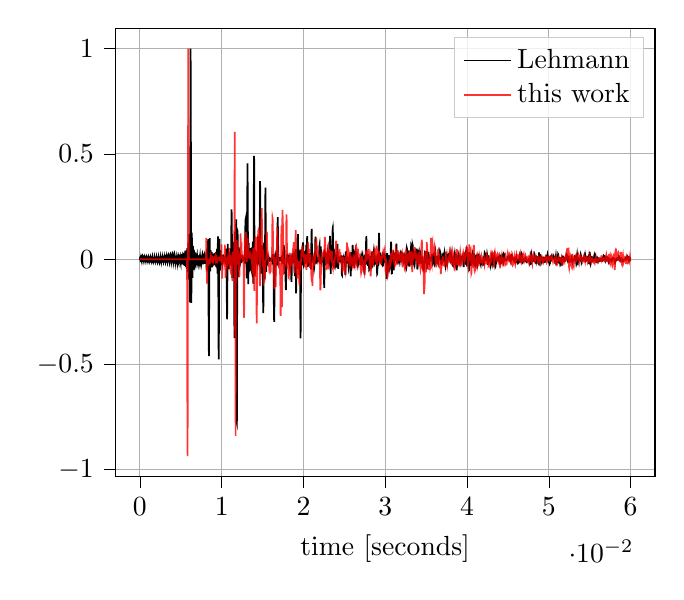
\begin{tikzpicture}

\begin{axis}[
legend cell align={left},
legend style={fill opacity=0.8, draw opacity=1, text opacity=1, draw=white!80.00000!black},
tick align=outside,
tick pos=left,
x grid style={white!69.01961!black},
xlabel={time [seconds]},
xmajorgrids,
xmin=-0.00300, xmax=0.06298,
xtick style={color=black},
y grid style={white!69.01961!black},
ymajorgrids,
ymin=-1.03223, ymax=1.09677,
ytick style={color=black}
]
\addplot [semithick, black]
table {%
0.00000 -0.00417
0.00002 0.00715
0.00005 0.00938
0.00007 0.00061
0.00009 -0.00894
0.00011 -0.00852
0.00014 0.00107
0.00016 0.00872
0.00018 0.00576
0.00020 -0.00420
0.00023 -0.00964
0.00025 -0.00441
0.00027 0.00533
0.00029 0.00832
0.00032 0.00121
0.00034 -0.00768
0.00036 -0.00810
0.00039 0.00035
0.00041 0.00784
0.00043 0.00572
0.00045 -0.00348
0.00048 -0.00907
0.00050 -0.00461
0.00052 0.00467
0.00054 0.00800
0.00057 0.00156
0.00059 -0.00714
0.00061 -0.00801
0.00063 -0.00006
0.00066 0.00744
0.00068 0.00579
0.00070 -0.00305
0.00073 -0.00881
0.00075 -0.00480
0.00077 0.00429
0.00079 0.00790
0.00082 0.00183
0.00084 -0.00684
0.00086 -0.00803
0.00088 -0.00036
0.00091 0.00724
0.00093 0.00592
0.00095 -0.00278
0.00098 -0.00873
0.00100 -0.00500
0.00102 0.00407
0.00104 0.00792
0.00107 0.00206
0.00109 -0.00670
0.00111 -0.00815
0.00113 -0.00058
0.00116 0.00721
0.00118 0.00611
0.00120 -0.00261
0.00122 -0.00881
0.00125 -0.00522
0.00127 0.00401
0.00129 0.00812
0.00132 0.00226
0.00134 -0.00679
0.00136 -0.00844
0.00138 -0.00068
0.00141 0.00751
0.00143 0.00648
0.00145 -0.00281
0.00147 -0.00976
0.00150 -0.00634
0.00152 0.00364
0.00154 0.00880
0.00156 0.00330
0.00159 -0.00643
0.00161 -0.00914
0.00163 -0.00174
0.00166 0.00716
0.00168 0.00723
0.00170 -0.00157
0.00172 -0.00901
0.00175 -0.00645
0.00177 0.00312
0.00179 0.00857
0.00181 0.00355
0.00184 -0.00608
0.00186 -0.00912
0.00188 -0.00202
0.00190 0.00695
0.00193 0.00735
0.00195 -0.00131
0.00197 -0.00894
0.00200 -0.00664
0.00202 0.00292
0.00204 0.00861
0.00206 0.00378
0.00209 -0.00597
0.00211 -0.00927
0.00213 -0.00223
0.00215 0.00695
0.00218 0.00756
0.00220 -0.00116
0.00222 -0.00906
0.00224 -0.00688
0.00227 0.00287
0.00229 0.00884
0.00231 0.00400
0.00234 -0.00606
0.00236 -0.00958
0.00238 -0.00237
0.00240 0.00721
0.00243 0.00793
0.00245 -0.00118
0.00247 -0.00955
0.00249 -0.00726
0.00252 0.00328
0.00254 0.01001
0.00256 0.00507
0.00259 -0.00599
0.00261 -0.01051
0.00263 -0.00335
0.00265 0.00717
0.00268 0.00885
0.00270 -0.00024
0.00272 -0.00954
0.00274 -0.00821
0.00277 0.00220
0.00279 0.00958
0.00281 0.00531
0.00283 -0.00566
0.00286 -0.01054
0.00288 -0.00361
0.00290 0.00709
0.00293 0.00906
0.00295 -0.00006
0.00297 -0.00966
0.00299 -0.00849
0.00302 0.00216
0.00304 0.00987
0.00306 0.00557
0.00308 -0.00582
0.00311 -0.01099
0.00313 -0.00376
0.00315 0.00753
0.00317 0.00963
0.00320 -0.00020
0.00322 -0.01075
0.00324 -0.00977
0.00327 0.00178
0.00329 0.01068
0.00331 0.00670
0.00333 -0.00554
0.00336 -0.01182
0.00338 -0.00481
0.00340 0.00735
0.00342 0.01047
0.00345 0.00088
0.00347 -0.01029
0.00349 -0.00996
0.00351 0.00157
0.00354 0.01087
0.00356 0.00699
0.00358 -0.00565
0.00361 -0.01228
0.00363 -0.00501
0.00365 0.00781
0.00367 0.01113
0.00370 0.00077
0.00372 -0.01147
0.00374 -0.01135
0.00376 0.00122
0.00379 0.01182
0.00381 0.00819
0.00383 -0.00549
0.00385 -0.01330
0.00388 -0.00607
0.00390 0.00786
0.00392 0.01220
0.00395 0.00172
0.00397 -0.01145
0.00399 -0.01179
0.00401 0.00142
0.00404 0.01303
0.00406 0.00945
0.00408 -0.00541
0.00410 -0.01445
0.00413 -0.00714
0.00415 0.00806
0.00417 0.01344
0.00420 0.00258
0.00422 -0.01192
0.00424 -0.01305
0.00426 0.00074
0.00429 0.01341
0.00431 0.00992
0.00433 -0.00605
0.00435 -0.01606
0.00438 -0.00823
0.00440 0.00864
0.00442 0.01501
0.00444 0.00332
0.00447 -0.01295
0.00449 -0.01467
0.00451 0.00056
0.00454 0.01526
0.00456 0.01216
0.00458 -0.00547
0.00460 -0.01730
0.00463 -0.00940
0.00465 0.00923
0.00467 0.01678
0.00469 0.00401
0.00472 -0.01456
0.00474 -0.01721
0.00476 -0.00041
0.00478 0.01657
0.00481 0.01374
0.00483 -0.00606
0.00485 -0.01997
0.00488 -0.01145
0.00490 0.01004
0.00492 0.01952
0.00494 0.00549
0.00497 -0.01614
0.00499 -0.02003
0.00501 -0.00110
0.00503 0.01895
0.00506 0.01641
0.00508 -0.00643
0.00510 -0.02315
0.00512 -0.01362
0.00515 0.01190
0.00517 0.02385
0.00519 0.00756
0.00522 -0.01877
0.00524 -0.02438
0.00526 -0.00185
0.00528 0.02324
0.00531 0.02126
0.00533 -0.00653
0.00535 -0.02817
0.00537 -0.01768
0.00540 0.01386
0.00542 0.02978
0.00544 0.01025
0.00546 -0.02328
0.00549 -0.03149
0.00551 -0.00320
0.00553 0.02975
0.00556 0.02806
0.00558 -0.00844
0.00560 -0.03814
0.00562 -0.02479
0.00565 0.01862
0.00567 0.04193
0.00569 0.01537
0.00571 -0.03298
0.00574 -0.04626
0.00576 -0.00497
0.00578 0.04603
0.00580 0.04557
0.00583 -0.01131
0.00585 -0.06127
0.00587 -0.04192
0.00590 0.03196
0.00592 0.07626
0.00594 0.03075
0.00596 -0.06312
0.00599 -0.09582
0.00601 -0.01228
0.00603 0.10840
0.00605 0.11919
0.00608 -0.03116
0.00610 -0.20503
0.00612 -0.17219
0.00615 0.17174
0.00617 0.67016
0.00619 1.00000
0.00621 0.92937
0.00624 0.51106
0.00626 0.03625
0.00628 -0.20770
0.00630 -0.15559
0.00633 0.02681
0.00635 0.12630
0.00637 0.07075
0.00639 -0.04487
0.00642 -0.08911
0.00644 -0.03088
0.00646 0.04948
0.00649 0.06293
0.00651 0.00575
0.00653 -0.05001
0.00655 -0.04416
0.00658 0.00887
0.00660 0.04528
0.00662 0.02710
0.00664 -0.01945
0.00667 -0.03988
0.00669 -0.01427
0.00671 0.02431
0.00673 0.03163
0.00676 0.00244
0.00678 -0.02724
0.00680 -0.02397
0.00683 0.00584
0.00685 0.02636
0.00687 0.01499
0.00689 -0.01306
0.00692 -0.02471
0.00694 -0.00772
0.00696 0.01675
0.00698 0.02032
0.00701 0.00012
0.00703 -0.01948
0.00705 -0.01623
0.00707 0.00471
0.00710 0.01822
0.00712 0.00915
0.00714 -0.01079
0.00717 -0.01789
0.00719 -0.00440
0.00721 0.01318
0.00723 0.01423
0.00726 -0.00186
0.00728 -0.01569
0.00730 -0.01116
0.00732 0.00588
0.00735 0.01507
0.00737 0.00573
0.00739 -0.01086
0.00741 -0.01516
0.00744 -0.00240
0.00746 0.01215
0.00748 0.01144
0.00751 -0.00331
0.00753 -0.01436
0.00755 -0.00862
0.00757 0.00690
0.00760 0.01360
0.00762 0.00344
0.00764 -0.01145
0.00766 -0.01318
0.00769 0.00052
0.00771 0.01338
0.00773 0.00982
0.00776 -0.00630
0.00778 -0.01583
0.00780 -0.00697
0.00782 0.01026
0.00785 0.01527
0.00787 0.00141
0.00789 -0.01532
0.00791 -0.01451
0.00794 0.00409
0.00796 0.01893
0.00798 0.01142
0.00800 -0.01119
0.00803 -0.02247
0.00805 -0.00742
0.00807 0.01805
0.00810 0.02337
0.00812 -0.00076
0.00814 -0.02820
0.00816 -0.02478
0.00819 0.01060
0.00821 0.03895
0.00823 0.02216
0.00825 -0.02927
0.00828 -0.05774
0.00830 -0.01764
0.00832 0.06429
0.00834 0.09532
0.00837 -0.00327
0.00839 -0.21202
0.00841 -0.40901
0.00844 -0.45989
0.00846 -0.32749
0.00848 -0.10349
0.00850 0.06675
0.00853 0.09936
0.00855 0.02658
0.00857 -0.05024
0.00859 -0.05737
0.00862 -0.00466
0.00864 0.04259
0.00866 0.03711
0.00868 -0.00711
0.00871 -0.03845
0.00873 -0.02552
0.00875 0.01302
0.00878 0.03346
0.00880 0.01548
0.00882 -0.01843
0.00884 -0.03032
0.00887 -0.00855
0.00889 0.02128
0.00891 0.02596
0.00893 0.00119
0.00896 -0.02482
0.00898 -0.02318
0.00900 0.00391
0.00902 0.02602
0.00905 0.01844
0.00907 -0.01046
0.00909 -0.02837
0.00912 -0.01487
0.00914 0.01545
0.00916 0.02857
0.00918 0.00883
0.00921 -0.02256
0.00923 -0.02995
0.00925 -0.00311
0.00927 0.02937
0.00930 0.03003
0.00932 -0.00495
0.00934 -0.03816
0.00937 -0.03002
0.00939 0.01531
0.00941 0.04891
0.00943 0.02785
0.00946 -0.03320
0.00948 -0.06795
0.00950 -0.02529
0.00952 0.06645
0.00955 0.10784
0.00957 0.01345
0.00959 -0.20027
0.00961 -0.40977
0.00964 -0.47555
0.00966 -0.35385
0.00968 -0.13105
0.00971 0.04862
0.00973 0.09657
0.00975 0.03627
0.00977 -0.03822
0.00980 -0.05353
0.00982 -0.01188
0.00984 0.03131
0.00986 0.03249
0.00989 -0.00055
0.00991 -0.02706
0.00993 -0.02079
0.00995 0.00577
0.00998 0.02113
0.01000 0.01085
0.01002 -0.00989
0.01005 -0.01711
0.01007 -0.00514
0.01009 0.00994
0.01011 0.01110
0.01014 -0.00068
0.01016 -0.01007
0.01018 -0.00677
0.01020 0.00329
0.01023 0.00709
0.01025 0.00105
0.01027 -0.00565
0.01029 -0.00393
0.01032 0.00310
0.01034 0.00467
0.01036 -0.00247
0.01039 -0.00833
0.01041 -0.00246
0.01043 0.01012
0.01045 0.01184
0.01048 -0.00523
0.01050 -0.02378
0.01052 -0.01595
0.01054 0.02143
0.01057 0.04958
0.01059 0.01566
0.01061 -0.09329
0.01063 -0.22306
0.01066 -0.28618
0.01068 -0.23323
0.01070 -0.09787
0.01073 0.02870
0.01075 0.07236
0.01077 0.03273
0.01079 -0.02770
0.01082 -0.04666
0.01084 -0.01531
0.01086 0.02530
0.01088 0.03298
0.01091 0.00539
0.01093 -0.02459
0.01095 -0.02702
0.01098 -0.00349
0.01100 0.02029
0.01102 0.02321
0.01104 0.00598
0.01107 -0.01624
0.01109 -0.02936
0.01111 -0.02380
0.01113 0.01097
0.01116 0.08179
0.01118 0.17284
0.01120 0.23678
0.01122 0.22098
0.01125 0.11697
0.01127 -0.01579
0.01129 -0.08836
0.01132 -0.05865
0.01134 0.02662
0.01136 0.07346
0.01138 0.03300
0.01141 -0.04723
0.01143 -0.07181
0.01145 -0.00360
0.01147 0.08251
0.01150 0.06450
0.01152 -0.09772
0.01154 -0.30007
0.01156 -0.37454
0.01159 -0.24636
0.01161 -0.01515
0.01163 0.12908
0.01166 0.08339
0.01168 -0.06885
0.01170 -0.14066
0.01172 -0.03302
0.01175 0.15104
0.01177 0.18939
0.01179 -0.04865
0.01181 -0.46081
0.01184 -0.77762
0.01186 -0.78101
0.01188 -0.48079
0.01190 -0.09542
0.01193 0.13544
0.01195 0.13328
0.01197 0.00557
0.01200 -0.08399
0.01202 -0.06275
0.01204 0.01622
0.01206 0.05870
0.01209 0.03028
0.01211 -0.02392
0.01213 -0.04214
0.01215 -0.01242
0.01218 0.02475
0.01220 0.02841
0.01222 0.00029
0.01224 -0.02419
0.01227 -0.01919
0.01229 0.00538
0.01231 0.02007
0.01234 0.01052
0.01236 -0.00933
0.01238 -0.01661
0.01240 -0.00560
0.01243 0.00880
0.01245 0.01055
0.01247 0.00002
0.01249 -0.00929
0.01252 -0.00781
0.01254 0.00063
0.01256 0.00583
0.01259 0.00369
0.01261 -0.00124
0.01263 -0.00356
0.01265 -0.00315
0.01268 -0.00232
0.01270 -0.00053
0.01272 0.00383
0.01274 0.00708
0.01277 0.00136
0.01279 -0.01352
0.01281 -0.02102
0.01283 0.00225
0.01286 0.06245
0.01288 0.13569
0.01290 0.18455
0.01293 0.19037
0.01295 0.16656
0.01297 0.13684
0.01299 0.10362
0.01302 0.04777
0.01304 -0.03307
0.01306 -0.09156
0.01308 -0.05344
0.01311 0.10944
0.01313 0.32531
0.01315 0.45525
0.01317 0.40077
0.01320 0.19291
0.01322 -0.02580
0.01324 -0.11817
0.01327 -0.06335
0.01329 0.04008
0.01331 0.07739
0.01333 0.02362
0.01336 -0.04880
0.01338 -0.05856
0.01340 -0.00190
0.01342 0.05160
0.01345 0.04156
0.01347 -0.01677
0.01349 -0.05388
0.01351 -0.02722
0.01354 0.03088
0.01356 0.05180
0.01358 0.01045
0.01361 -0.04510
0.01363 -0.04887
0.01365 0.00579
0.01367 0.05590
0.01370 0.04014
0.01372 -0.02777
0.01374 -0.06941
0.01376 -0.02963
0.01379 0.05403
0.01381 0.08340
0.01383 0.00792
0.01385 -0.10450
0.01388 -0.11726
0.01390 0.04350
0.01392 0.30364
0.01395 0.49054
0.01397 0.47594
0.01399 0.28070
0.01401 0.04822
0.01404 -0.08071
0.01406 -0.07301
0.01408 -0.00141
0.01410 0.04298
0.01413 0.02968
0.01415 -0.00750
0.01417 -0.02473
0.01420 -0.01331
0.01422 0.00478
0.01424 0.01053
0.01426 0.00597
0.01429 0.00162
0.01431 -0.00153
0.01433 -0.00932
0.01435 -0.01736
0.01438 -0.00773
0.01440 0.03059
0.01442 0.08137
0.01444 0.10938
0.01447 0.09345
0.01449 0.04810
0.01451 0.00788
0.01454 -0.00890
0.01456 -0.01426
0.01458 -0.02464
0.01460 -0.02612
0.01463 0.02232
0.01465 0.14120
0.01467 0.28753
0.01469 0.37060
0.01472 0.32413
0.01474 0.16958
0.01476 0.00618
0.01478 -0.06895
0.01481 -0.03848
0.01483 0.03068
0.01485 0.05660
0.01488 0.01677
0.01490 -0.04084
0.01492 -0.05343
0.01494 -0.00667
0.01497 0.05360
0.01499 0.06520
0.01501 0.00255
0.01503 -0.10723
0.01506 -0.20918
0.01508 -0.25619
0.01510 -0.22909
0.01512 -0.13905
0.01515 -0.02331
0.01517 0.06490
0.01519 0.08016
0.01522 0.01812
0.01524 -0.06835
0.01526 -0.09634
0.01528 -0.01436
0.01531 0.14941
0.01533 0.29887
0.01535 0.33938
0.01537 0.24969
0.01540 0.09532
0.01542 -0.02646
0.01544 -0.06072
0.01546 -0.02566
0.01549 0.01909
0.01551 0.02954
0.01553 0.00745
0.01556 -0.01602
0.01558 -0.01764
0.01560 -0.00173
0.01562 0.01134
0.01565 0.00916
0.01567 -0.00247
0.01569 -0.00971
0.01571 -0.00634
0.01574 0.00186
0.01576 0.00574
0.01578 0.00256
0.01580 -0.00294
0.01583 -0.00499
0.01585 -0.00247
0.01587 0.00140
0.01590 0.00310
0.01592 0.00170
0.01594 -0.00131
0.01596 -0.00354
0.01599 -0.00319
0.01601 -0.00032
0.01603 0.00274
0.01605 0.00271
0.01608 -0.00120
0.01610 -0.00539
0.01612 -0.00467
0.01615 0.00164
0.01617 0.00708
0.01619 0.00403
0.01621 -0.00662
0.01624 -0.01302
0.01626 -0.00360
0.01628 0.01687
0.01630 0.02343
0.01633 -0.01234
0.01635 -0.09667
0.01637 -0.20179
0.01639 -0.28068
0.01642 -0.29770
0.01644 -0.25040
0.01646 -0.16647
0.01649 -0.08208
0.01651 -0.02141
0.01653 0.00910
0.01655 0.01451
0.01658 0.00456
0.01660 -0.00866
0.01662 -0.01313
0.01664 -0.00382
0.01667 0.01123
0.01669 0.01546
0.01671 -0.00004
0.01673 -0.02275
0.01676 -0.02363
0.01678 0.01902
0.01680 0.09665
0.01683 0.17078
0.01685 0.19931
0.01687 0.16742
0.01689 0.09707
0.01692 0.02840
0.01694 -0.00950
0.01696 -0.01422
0.01698 -0.00299
0.01701 0.00595
0.01703 0.00588
0.01705 0.00065
0.01707 -0.00356
0.01710 -0.00400
0.01712 -0.00154
0.01714 0.00172
0.01717 0.00358
0.01719 0.00242
0.01721 -0.00149
0.01723 -0.00501
0.01726 -0.00426
0.01728 0.00098
0.01730 0.00567
0.01732 0.00397
0.01735 -0.00381
0.01737 -0.00985
0.01739 -0.00627
0.01741 0.00534
0.01744 0.01336
0.01746 0.00715
0.01748 -0.01037
0.01751 -0.02216
0.01753 -0.01140
0.01755 0.02168
0.01757 0.05657
0.01760 0.06719
0.01762 0.04223
0.01764 -0.00585
0.01766 -0.05028
0.01769 -0.06919
0.01771 -0.05969
0.01773 -0.03791
0.01776 -0.02707
0.01778 -0.04243
0.01780 -0.08166
0.01782 -0.12526
0.01785 -0.14720
0.01787 -0.13095
0.01789 -0.08140
0.01791 -0.02328
0.01794 0.01492
0.01796 0.02065
0.01798 0.00469
0.01800 -0.01032
0.01803 -0.01000
0.01805 0.00127
0.01807 0.00857
0.01810 0.00377
0.01812 -0.00629
0.01814 -0.00880
0.01816 -0.00033
0.01819 0.00887
0.01821 0.00684
0.01823 -0.00546
0.01825 -0.01384
0.01828 -0.00649
0.01830 0.01111
0.01832 0.01939
0.01834 0.00412
0.01837 -0.02781
0.01839 -0.05355
0.01841 -0.05663
0.01844 -0.04376
0.01846 -0.03841
0.01848 -0.05662
0.01850 -0.08897
0.01853 -0.10711
0.01855 -0.08947
0.01857 -0.04180
0.01859 0.00668
0.01862 0.02768
0.01864 0.01650
0.01866 -0.00707
0.01868 -0.01844
0.01871 -0.00957
0.01873 0.00700
0.01875 0.01320
0.01878 0.00399
0.01880 -0.00857
0.01882 -0.00921
0.01884 0.00258
0.01887 0.00921
0.01889 -0.00820
0.01891 -0.04739
0.01893 -0.07981
0.01896 -0.07265
0.01898 -0.02165
0.01900 0.03620
0.01902 0.04777
0.01905 -0.00984
0.01907 -0.10267
0.01909 -0.16191
0.01912 -0.14064
0.01914 -0.05594
0.01916 0.02435
0.01918 0.04168
0.01921 -0.00096
0.01923 -0.04419
0.01925 -0.03083
0.01927 0.03851
0.01930 0.10711
0.01932 0.11866
0.01934 0.07116
0.01937 0.01429
0.01939 -0.00523
0.01941 0.00891
0.01943 0.01285
0.01946 -0.02159
0.01948 -0.06864
0.01950 -0.07379
0.01952 -0.01930
0.01955 0.04131
0.01957 0.02415
0.01959 -0.10229
0.01961 -0.27402
0.01964 -0.37596
0.01966 -0.33687
0.01968 -0.18770
0.01971 -0.03099
0.01973 0.04648
0.01975 0.03575
0.01977 -0.00788
0.01980 -0.02865
0.01982 -0.01633
0.01984 0.00374
0.01986 0.01234
0.01989 0.01798
0.01991 0.03786
0.01993 0.06764
0.01995 0.07988
0.01998 0.05447
0.02000 0.00501
0.02002 -0.03090
0.02005 -0.02812
0.02007 0.00245
0.02009 0.02815
0.02011 0.02924
0.02014 0.01531
0.02016 0.00787
0.02018 0.01257
0.02020 0.01462
0.02023 0.00138
0.02025 -0.01720
0.02027 -0.01694
0.02029 0.01190
0.02032 0.05005
0.02034 0.06823
0.02036 0.05965
0.02039 0.04819
0.02041 0.06054
0.02043 0.09261
0.02045 0.10939
0.02048 0.08154
0.02050 0.01990
0.02052 -0.03097
0.02054 -0.03564
0.02057 -0.00242
0.02059 0.02705
0.02061 0.02183
0.02063 -0.00810
0.02066 -0.02659
0.02068 -0.01318
0.02070 0.01484
0.02073 0.02381
0.02075 0.00305
0.02077 -0.02266
0.02079 -0.02186
0.02082 0.00633
0.02084 0.02909
0.02086 0.01605
0.02088 -0.02414
0.02091 -0.04774
0.02093 -0.01820
0.02095 0.05581
0.02098 0.12546
0.02100 0.14425
0.02102 0.10606
0.02104 0.04437
0.02107 -0.00133
0.02109 -0.01603
0.02111 -0.01068
0.02113 -0.00186
0.02116 0.00404
0.02118 0.00822
0.02120 0.00888
0.02122 -0.00013
0.02125 -0.01974
0.02127 -0.03984
0.02129 -0.04731
0.02132 -0.03939
0.02134 -0.02577
0.02136 -0.01543
0.02138 -0.00420
0.02141 0.02045
0.02143 0.06086
0.02145 0.09855
0.02147 0.10671
0.02150 0.07559
0.02152 0.02450
0.02154 -0.01360
0.02156 -0.02021
0.02159 -0.00458
0.02161 0.00972
0.02163 0.00888
0.02166 -0.00132
0.02168 -0.00717
0.02170 -0.00386
0.02172 0.00166
0.02175 0.00212
0.02177 -0.00075
0.02179 -0.00058
0.02181 0.00268
0.02184 0.00152
0.02186 -0.00750
0.02188 -0.01407
0.02190 -0.00197
0.02193 0.03108
0.02195 0.06404
0.02197 0.06858
0.02200 0.03721
0.02202 -0.00551
0.02204 -0.02332
0.02206 -0.00175
0.02209 0.03830
0.02211 0.06081
0.02213 0.04813
0.02215 0.01461
0.02218 -0.01098
0.02220 -0.01361
0.02222 -0.00197
0.02224 0.00631
0.02227 0.00433
0.02229 -0.00114
0.02231 -0.00249
0.02234 -0.00124
0.02236 -0.00280
0.02238 -0.00526
0.02240 -0.00018
0.02243 0.01289
0.02245 0.01682
0.02247 -0.01020
0.02249 -0.06822
0.02252 -0.12461
0.02254 -0.13652
0.02256 -0.08970
0.02259 -0.01540
0.02261 0.03456
0.02263 0.03271
0.02265 -0.00229
0.02268 -0.02772
0.02270 -0.01937
0.02272 0.00834
0.02274 0.02278
0.02277 0.00970
0.02279 -0.01342
0.02281 -0.01943
0.02283 -0.00245
0.02286 0.01664
0.02288 0.01507
0.02290 -0.00559
0.02293 -0.02105
0.02295 -0.01139
0.02297 0.01692
0.02299 0.03825
0.02302 0.03524
0.02304 0.01571
0.02306 0.00119
0.02308 0.00154
0.02311 0.00560
0.02313 -0.00151
0.02315 -0.01544
0.02317 -0.01255
0.02320 0.02386
0.02322 0.07856
0.02324 0.11028
0.02327 0.08703
0.02329 0.01808
0.02331 -0.04958
0.02333 -0.06910
0.02336 -0.03209
0.02338 0.02635
0.02340 0.05879
0.02342 0.04395
0.02345 0.00063
0.02347 -0.03080
0.02349 -0.02033
0.02351 0.03185
0.02354 0.09860
0.02356 0.14505
0.02358 0.14885
0.02361 0.11053
0.02363 0.05081
0.02365 -0.00241
0.02367 -0.03033
0.02370 -0.03305
0.02372 -0.02584
0.02374 -0.02415
0.02376 -0.02990
0.02379 -0.03161
0.02381 -0.01863
0.02383 0.00481
0.02385 0.02101
0.02388 0.01584
0.02390 -0.00561
0.02392 -0.02195
0.02395 -0.01589
0.02397 0.00756
0.02399 0.02445
0.02401 0.01496
0.02404 -0.01568
0.02406 -0.03969
0.02408 -0.03124
0.02410 0.00947
0.02413 0.05500
0.02415 0.07307
0.02417 0.05207
0.02420 0.00792
0.02422 -0.03109
0.02424 -0.04585
0.02426 -0.03654
0.02429 -0.01651
0.02431 0.00040
0.02433 0.00778
0.02435 0.00639
0.02438 0.00042
0.02440 -0.00513
0.02442 -0.00610
0.02444 -0.00145
0.02447 0.00502
0.02449 0.00681
0.02451 0.00091
0.02454 -0.00775
0.02456 -0.00947
0.02458 0.00021
0.02460 0.01334
0.02463 0.01381
0.02465 -0.00842
0.02467 -0.04565
0.02469 -0.07547
0.02472 -0.07760
0.02474 -0.05058
0.02476 -0.01322
0.02478 0.01078
0.02481 0.01157
0.02483 -0.00120
0.02485 -0.00988
0.02488 -0.00572
0.02490 0.00459
0.02492 0.00819
0.02494 0.00067
0.02497 -0.00891
0.02499 -0.00798
0.02501 0.00472
0.02503 0.01503
0.02506 0.00559
0.02508 -0.02626
0.02510 -0.06224
0.02512 -0.07597
0.02515 -0.05479
0.02517 -0.01116
0.02519 0.02691
0.02522 0.03806
0.02524 0.02307
0.02526 0.00074
0.02528 -0.01036
0.02531 -0.00665
0.02533 0.00187
0.02535 0.00485
0.02537 0.00181
0.02540 -0.00061
0.02542 0.00066
0.02544 0.00016
0.02546 -0.00915
0.02549 -0.02519
0.02551 -0.03563
0.02553 -0.02955
0.02556 -0.00982
0.02558 0.00800
0.02560 0.01067
0.02562 0.00071
0.02565 -0.00690
0.02567 -0.00237
0.02569 0.00591
0.02571 -0.00129
0.02574 -0.03187
0.02576 -0.06864
0.02578 -0.08097
0.02580 -0.05337
0.02583 -0.00327
0.02585 0.03159
0.02587 0.02646
0.02590 -0.00760
0.02592 -0.03371
0.02594 -0.02327
0.02596 0.01834
0.02599 0.05829
0.02601 0.06792
0.02603 0.04823
0.02605 0.02544
0.02608 0.02292
0.02610 0.03832
0.02612 0.04791
0.02615 0.03217
0.02617 -0.00391
0.02619 -0.03550
0.02621 -0.04168
0.02624 -0.02386
0.02626 -0.00186
0.02628 0.00672
0.02630 0.00222
0.02633 -0.00090
0.02635 0.00841
0.02637 0.02545
0.02639 0.03450
0.02642 0.02503
0.02644 0.00246
0.02646 -0.01644
0.02649 -0.01851
0.02651 -0.00508
0.02653 0.01045
0.02655 0.01451
0.02658 0.00371
0.02660 -0.01440
0.02662 -0.02865
0.02664 -0.03223
0.02667 -0.02559
0.02669 -0.01405
0.02671 -0.00354
0.02673 0.00233
0.02676 0.00315
0.02678 0.00113
0.02680 -0.00066
0.02683 -0.00050
0.02685 0.00047
0.02687 -0.00091
0.02689 -0.00694
0.02692 -0.01622
0.02694 -0.02362
0.02696 -0.02371
0.02698 -0.01479
0.02701 -0.00058
0.02703 0.01199
0.02705 0.01688
0.02707 0.01219
0.02710 0.00090
0.02712 -0.01069
0.02714 -0.01585
0.02717 -0.01089
0.02719 0.00213
0.02721 0.01536
0.02723 0.01945
0.02726 0.01065
0.02728 -0.00481
0.02730 -0.01412
0.02732 -0.00850
0.02735 0.00722
0.02737 0.01595
0.02739 0.00215
0.02741 -0.03242
0.02744 -0.06606
0.02746 -0.07287
0.02748 -0.04534
0.02751 -0.00329
0.02753 0.02113
0.02755 0.01152
0.02757 -0.01664
0.02760 -0.02808
0.02762 0.00061
0.02764 0.05777
0.02766 0.10396
0.02769 0.10477
0.02771 0.06033
0.02773 0.00476
0.02776 -0.02379
0.02778 -0.01498
0.02780 0.00856
0.02782 0.01600
0.02785 -0.00201
0.02787 -0.02659
0.02789 -0.03169
0.02791 -0.01084
0.02794 0.01661
0.02796 0.02449
0.02798 0.00416
0.02800 -0.02896
0.02803 -0.05092
0.02805 -0.04974
0.02807 -0.03171
0.02810 -0.01095
0.02812 0.00365
0.02814 0.01099
0.02816 0.01107
0.02819 0.00111
0.02821 -0.01927
0.02823 -0.04071
0.02825 -0.04693
0.02828 -0.02861
0.02830 0.00503
0.02832 0.03090
0.02834 0.03123
0.02837 0.00954
0.02839 -0.01286
0.02841 -0.01681
0.02844 -0.00254
0.02846 0.01250
0.02848 0.01215
0.02850 -0.00256
0.02853 -0.01539
0.02855 -0.01132
0.02857 0.00947
0.02859 0.03297
0.02862 0.04436
0.02864 0.03901
0.02866 0.02256
0.02868 0.00373
0.02871 -0.01113
0.02873 -0.01830
0.02875 -0.01587
0.02878 -0.00574
0.02880 0.00478
0.02882 0.00705
0.02884 -0.00038
0.02887 -0.00850
0.02889 -0.00616
0.02891 0.00605
0.02893 0.01240
0.02896 -0.00388
0.02898 -0.04050
0.02900 -0.07210
0.02902 -0.07069
0.02905 -0.03334
0.02907 0.01099
0.02909 0.02591
0.02912 0.00240
0.02914 -0.03018
0.02916 -0.02972
0.02918 0.01866
0.02921 0.08638
0.02923 0.12494
0.02925 0.10790
0.02927 0.05249
0.02930 0.00219
0.02932 -0.01166
0.02934 0.00668
0.02937 0.02779
0.02939 0.02756
0.02941 0.00744
0.02943 -0.01215
0.02946 -0.01457
0.02948 -0.00203
0.02950 0.00948
0.02952 0.00726
0.02955 -0.00698
0.02957 -0.02067
0.02959 -0.02256
0.02961 -0.01152
0.02964 0.00408
0.02966 0.01323
0.02968 0.00931
0.02971 -0.00633
0.02973 -0.02466
0.02975 -0.03339
0.02977 -0.02460
0.02980 -0.00147
0.02982 0.02210
0.02984 0.03099
0.02986 0.02086
0.02989 0.00181
0.02991 -0.01065
0.02993 -0.00939
0.02995 -0.00072
0.02998 0.00414
0.03000 0.00167
0.03002 -0.00124
0.03005 0.00224
0.03007 0.00732
0.03009 -0.00062
0.03011 -0.03019
0.03014 -0.07016
0.03016 -0.09385
0.03018 -0.08074
0.03020 -0.03606
0.03023 0.01070
0.03025 0.02843
0.03027 0.00868
0.03029 -0.02920
0.03032 -0.05515
0.03034 -0.05171
0.03036 -0.02464
0.03039 0.00518
0.03041 0.01869
0.03043 0.01052
0.03045 -0.01079
0.03048 -0.03091
0.03050 -0.03918
0.03052 -0.03435
0.03054 -0.02415
0.03057 -0.01888
0.03059 -0.02214
0.03061 -0.02583
0.03063 -0.01546
0.03066 0.01603
0.03068 0.05730
0.03070 0.08261
0.03073 0.07071
0.03075 0.02352
0.03077 -0.03292
0.03079 -0.06750
0.03082 -0.06691
0.03084 -0.04213
0.03086 -0.01444
0.03088 0.00366
0.03091 0.01389
0.03093 0.02155
0.03095 0.02375
0.03098 0.01160
0.03100 -0.01603
0.03102 -0.04442
0.03104 -0.05271
0.03107 -0.03343
0.03109 -0.00132
0.03111 0.01920
0.03113 0.01641
0.03116 0.00079
0.03118 -0.00769
0.03120 -0.00052
0.03122 0.01248
0.03125 0.01697
0.03127 0.01224
0.03129 0.01271
0.03132 0.03053
0.03134 0.05864
0.03136 0.07402
0.03138 0.05961
0.03141 0.02242
0.03143 -0.01139
0.03145 -0.02023
0.03147 -0.00583
0.03150 0.01109
0.03152 0.01255
0.03154 -0.00024
0.03156 -0.01139
0.03159 -0.00897
0.03161 0.00295
0.03163 0.01044
0.03166 0.00560
0.03168 -0.00562
0.03170 -0.01110
0.03172 -0.00567
0.03175 0.00497
0.03177 0.01253
0.03179 0.01552
0.03181 0.01866
0.03184 0.02421
0.03186 0.02695
0.03188 0.02002
0.03190 0.00518
0.03193 -0.00564
0.03195 -0.00124
0.03197 0.01637
0.03200 0.03197
0.03202 0.03115
0.03204 0.01461
0.03206 -0.00216
0.03209 -0.00403
0.03211 0.00917
0.03213 0.02309
0.03215 0.02355
0.03218 0.01017
0.03220 -0.00456
0.03222 -0.00862
0.03224 -0.00199
0.03227 0.00515
0.03229 0.00427
0.03231 -0.00263
0.03234 -0.00621
0.03236 -0.00055
0.03238 0.01032
0.03240 0.01657
0.03243 0.01220
0.03245 -0.00016
0.03247 -0.01363
0.03249 -0.02437
0.03252 -0.03340
0.03254 -0.04136
0.03256 -0.04341
0.03259 -0.03164
0.03261 -0.00406
0.03263 0.02915
0.03265 0.04982
0.03268 0.04488
0.03270 0.01743
0.03272 -0.01412
0.03274 -0.02885
0.03277 -0.01815
0.03279 0.00903
0.03281 0.03368
0.03283 0.04038
0.03286 0.02666
0.03288 0.00206
0.03290 -0.02011
0.03293 -0.03141
0.03295 -0.03131
0.03297 -0.02453
0.03299 -0.01638
0.03302 -0.00974
0.03304 -0.00440
0.03306 0.00204
0.03308 0.01269
0.03311 0.02891
0.03313 0.04757
0.03315 0.06028
0.03317 0.05725
0.03320 0.03508
0.03322 0.00264
0.03324 -0.02135
0.03327 -0.02010
0.03329 0.00810
0.03331 0.04644
0.03333 0.07042
0.03336 0.06563
0.03338 0.03818
0.03340 0.00894
0.03342 -0.00337
0.03345 0.00386
0.03347 0.01752
0.03349 0.02156
0.03351 0.01016
0.03354 -0.00948
0.03356 -0.02488
0.03358 -0.02804
0.03361 -0.01892
0.03363 -0.00255
0.03365 0.01501
0.03367 0.02835
0.03370 0.03325
0.03372 0.02893
0.03374 0.02059
0.03376 0.01765
0.03379 0.02622
0.03381 0.04158
0.03383 0.04931
0.03385 0.03649
0.03388 0.00416
0.03390 -0.03102
0.03392 -0.04865
0.03395 -0.03999
0.03397 -0.01329
0.03399 0.01478
0.03401 0.03235
0.03404 0.03811
0.03406 0.03654
0.03408 0.03058
0.03410 0.02060
0.03413 0.00910
0.03415 0.00280
0.03417 0.00724
0.03420 0.01917
0.03422 0.02691
0.03424 0.02078
0.03426 0.00373
0.03429 -0.00998
0.03431 -0.00857
0.03433 0.00477
0.03435 0.01423
0.03438 0.00743
0.03440 -0.01115
0.03442 -0.02385
0.03444 -0.01779
0.03447 0.00116
0.03449 0.01313
0.03451 0.00356
0.03454 -0.02219
0.03456 -0.04374
0.03458 -0.04503
0.03460 -0.02887
0.03463 -0.01298
0.03465 -0.01266
0.03467 -0.02749
0.03469 -0.04390
0.03472 -0.04854
0.03474 -0.03841
0.03476 -0.01957
0.03478 0.00049
0.03481 0.01706
0.03483 0.02643
0.03485 0.02430
0.03488 0.00978
0.03490 -0.00903
0.03492 -0.01720
0.03494 -0.00500
0.03497 0.02057
0.03499 0.03816
0.03501 0.02943
0.03503 -0.00346
0.03506 -0.03769
0.03508 -0.04872
0.03510 -0.03143
0.03512 -0.00364
0.03515 0.01106
0.03517 0.00472
0.03519 -0.00957
0.03522 -0.01225
0.03524 0.00323
0.03526 0.02473
0.03528 0.03371
0.03531 0.02252
0.03533 0.00029
0.03535 -0.01671
0.03537 -0.01935
0.03540 -0.01139
0.03542 -0.00309
0.03544 -0.00091
0.03546 -0.00324
0.03549 -0.00445
0.03551 -0.00156
0.03553 0.00348
0.03556 0.00701
0.03558 0.00789
0.03560 0.00827
0.03562 0.01062
0.03565 0.01449
0.03567 0.01622
0.03569 0.01210
0.03571 0.00216
0.03574 -0.00868
0.03576 -0.01337
0.03578 -0.00795
0.03580 0.00475
0.03583 0.01623
0.03585 0.01814
0.03587 0.00871
0.03590 -0.00593
0.03592 -0.01712
0.03594 -0.02107
0.03596 -0.02121
0.03599 -0.02294
0.03601 -0.02613
0.03603 -0.02368
0.03605 -0.00891
0.03608 0.01533
0.03610 0.03587
0.03612 0.03929
0.03615 0.02410
0.03617 0.00279
0.03619 -0.00901
0.03621 -0.00630
0.03624 0.00202
0.03626 0.00335
0.03628 -0.00532
0.03630 -0.01470
0.03633 -0.01353
0.03635 -0.00106
0.03637 0.01155
0.03639 0.01213
0.03642 -0.00027
0.03644 -0.01452
0.03646 -0.01820
0.03649 -0.00898
0.03651 0.00443
0.03653 0.01186
0.03655 0.01122
0.03658 0.00903
0.03660 0.01267
0.03662 0.02305
0.03664 0.03442
0.03667 0.04003
0.03669 0.03699
0.03671 0.02662
0.03673 0.01208
0.03676 -0.00311
0.03678 -0.01518
0.03680 -0.02113
0.03683 -0.02115
0.03685 -0.01938
0.03687 -0.02031
0.03689 -0.02342
0.03692 -0.02240
0.03694 -0.01165
0.03696 0.00593
0.03698 0.01882
0.03701 0.01687
0.03703 0.00210
0.03705 -0.01153
0.03707 -0.01086
0.03710 0.00312
0.03712 0.01572
0.03714 0.01333
0.03717 -0.00195
0.03719 -0.01347
0.03721 -0.00677
0.03723 0.01489
0.03726 0.03237
0.03728 0.02873
0.03730 0.00549
0.03732 -0.01911
0.03735 -0.02778
0.03737 -0.01968
0.03739 -0.00849
0.03741 -0.00659
0.03744 -0.01255
0.03746 -0.01475
0.03748 -0.00582
0.03751 0.00828
0.03753 0.01432
0.03755 0.00601
0.03757 -0.00908
0.03760 -0.01705
0.03762 -0.01096
0.03764 0.00356
0.03766 0.01517
0.03769 0.01756
0.03771 0.01295
0.03773 0.00696
0.03776 0.00248
0.03778 -0.00040
0.03780 -0.00047
0.03782 0.00514
0.03785 0.01625
0.03787 0.02574
0.03789 0.02390
0.03791 0.00846
0.03794 -0.01021
0.03796 -0.01660
0.03798 -0.00438
0.03800 0.01651
0.03803 0.02823
0.03805 0.02138
0.03807 0.00328
0.03810 -0.00987
0.03812 -0.00867
0.03814 0.00166
0.03816 0.00815
0.03819 0.00322
0.03821 -0.00957
0.03823 -0.02161
0.03825 -0.02835
0.03828 -0.03133
0.03830 -0.03254
0.03832 -0.02981
0.03834 -0.01980
0.03837 -0.00432
0.03839 0.00895
0.03841 0.01400
0.03844 0.01339
0.03846 0.01543
0.03848 0.02321
0.03850 0.02846
0.03853 0.01922
0.03855 -0.00514
0.03857 -0.02848
0.03859 -0.03077
0.03862 -0.00840
0.03864 0.01923
0.03866 0.02577
0.03868 0.00247
0.03871 -0.03310
0.03873 -0.05315
0.03875 -0.04528
0.03878 -0.02228
0.03880 -0.00728
0.03882 -0.01052
0.03884 -0.02125
0.03887 -0.02177
0.03889 -0.00717
0.03891 0.01018
0.03893 0.01489
0.03896 0.00502
0.03898 -0.00697
0.03900 -0.00881
0.03902 -0.00145
0.03905 0.00343
0.03907 -0.00231
0.03909 -0.01384
0.03912 -0.01901
0.03914 -0.01223
0.03916 -0.00052
0.03918 0.00445
0.03921 -0.00096
0.03923 -0.00918
0.03925 -0.01063
0.03927 -0.00401
0.03930 0.00359
0.03932 0.00595
0.03934 0.00462
0.03937 0.00560
0.03939 0.01070
0.03941 0.01474
0.03943 0.01214
0.03946 0.00437
0.03948 -0.00157
0.03950 -0.00249
0.03952 -0.00403
0.03955 -0.01381
0.03957 -0.02960
0.03959 -0.03741
0.03961 -0.02478
0.03964 0.00377
0.03966 0.02725
0.03968 0.02688
0.03971 0.00500
0.03973 -0.01636
0.03975 -0.01726
0.03977 0.00027
0.03980 0.01549
0.03982 0.01229
0.03984 -0.00248
0.03986 -0.00620
0.03989 0.01389
0.03991 0.04430
0.03993 0.05694
0.03995 0.03743
0.03998 0.00038
0.04000 -0.02503
0.04002 -0.02395
0.04005 -0.00876
0.04007 -0.00271
0.04009 -0.01306
0.04011 -0.02345
0.04014 -0.01413
0.04016 0.01274
0.04018 0.03157
0.04020 0.01909
0.04023 -0.01959
0.04025 -0.05293
0.04027 -0.05231
0.04029 -0.01897
0.04032 0.01857
0.04034 0.03302
0.04036 0.02284
0.04039 0.00862
0.04041 0.00785
0.04043 0.01661
0.04045 0.01700
0.04048 0.00010
0.04050 -0.02247
0.04052 -0.03089
0.04054 -0.01911
0.04057 -0.00122
0.04059 0.00445
0.04061 -0.00462
0.04063 -0.01353
0.04066 -0.00805
0.04068 0.00850
0.04070 0.01899
0.04073 0.01249
0.04075 -0.00243
0.04077 -0.00689
0.04079 0.00652
0.04082 0.02391
0.04084 0.02409
0.04086 0.00186
0.04088 -0.02493
0.04091 -0.03299
0.04093 -0.01767
0.04095 0.00221
0.04098 0.00404
0.04100 -0.01510
0.04102 -0.03560
0.04104 -0.03573
0.04107 -0.01355
0.04109 0.01215
0.04111 0.02153
0.04113 0.01270
0.04116 0.00077
0.04118 -0.00015
0.04120 0.00835
0.04122 0.01263
0.04125 0.00359
0.04127 -0.01280
0.04129 -0.02177
0.04132 -0.01517
0.04134 0.00094
0.04136 0.01348
0.04138 0.01532
0.04141 0.01008
0.04143 0.00521
0.04145 0.00312
0.04147 0.00047
0.04150 -0.00495
0.04152 -0.00946
0.04154 -0.00742
0.04156 0.00086
0.04159 0.00736
0.04161 0.00385
0.04163 -0.00912
0.04166 -0.02195
0.04168 -0.02523
0.04170 -0.01885
0.04172 -0.01126
0.04175 -0.01025
0.04177 -0.01529
0.04179 -0.01949
0.04181 -0.01810
0.04184 -0.01367
0.04186 -0.01223
0.04188 -0.01550
0.04190 -0.01831
0.04193 -0.01467
0.04195 -0.00531
0.04197 0.00168
0.04200 -0.00140
0.04202 -0.01367
0.04204 -0.02549
0.04206 -0.02644
0.04209 -0.01376
0.04211 0.00615
0.04213 0.02336
0.04215 0.03116
0.04218 0.02876
0.04220 0.01964
0.04222 0.00872
0.04224 0.00038
0.04227 -0.00297
0.04229 -0.00216
0.04231 -0.00083
0.04234 -0.00232
0.04236 -0.00581
0.04238 -0.00611
0.04240 0.00122
0.04243 0.01382
0.04245 0.02225
0.04247 0.01755
0.04249 0.00017
0.04252 -0.01885
0.04254 -0.02644
0.04256 -0.01844
0.04259 -0.00258
0.04261 0.00903
0.04263 0.01023
0.04265 0.00420
0.04268 -0.00213
0.04270 -0.00537
0.04272 -0.00713
0.04274 -0.00941
0.04277 -0.01082
0.04279 -0.00873
0.04281 -0.00429
0.04283 -0.00329
0.04286 -0.01038
0.04288 -0.02261
0.04290 -0.03019
0.04293 -0.02492
0.04295 -0.00809
0.04297 0.01054
0.04299 0.02181
0.04302 0.02468
0.04304 0.02474
0.04306 0.02581
0.04308 0.02487
0.04311 0.01603
0.04313 -0.00103
0.04315 -0.01814
0.04317 -0.02552
0.04320 -0.02128
0.04322 -0.01316
0.04324 -0.01023
0.04327 -0.01333
0.04329 -0.01458
0.04331 -0.00686
0.04333 0.00715
0.04336 0.01609
0.04338 0.01054
0.04340 -0.00781
0.04342 -0.02752
0.04345 -0.03761
0.04347 -0.03607
0.04349 -0.02909
0.04351 -0.02312
0.04354 -0.01912
0.04356 -0.01405
0.04358 -0.00646
0.04361 0.00112
0.04363 0.00534
0.04365 0.00614
0.04367 0.00653
0.04370 0.00830
0.04372 0.00949
0.04374 0.00698
0.04376 0.00119
0.04379 -0.00320
0.04381 -0.00219
0.04383 0.00251
0.04385 0.00458
0.04388 0.00003
0.04390 -0.00767
0.04392 -0.01051
0.04395 -0.00446
0.04397 0.00546
0.04399 0.00964
0.04401 0.00356
0.04404 -0.00724
0.04406 -0.01261
0.04408 -0.00791
0.04410 0.00146
0.04413 0.00585
0.04415 0.00104
0.04417 -0.00813
0.04420 -0.01352
0.04422 -0.01189
0.04424 -0.00685
0.04426 -0.00329
0.04429 -0.00143
0.04431 0.00228
0.04433 0.00895
0.04435 0.01358
0.04438 0.00944
0.04440 -0.00378
0.04442 -0.01706
0.04444 -0.01895
0.04447 -0.00608
0.04449 0.01305
0.04451 0.02512
0.04454 0.02323
0.04456 0.01178
0.04458 0.00098
0.04460 -0.00267
0.04463 -0.00073
0.04465 0.00108
0.04467 -0.00036
0.04469 -0.00324
0.04472 -0.00428
0.04474 -0.00311
0.04476 -0.00232
0.04478 -0.00386
0.04481 -0.00632
0.04483 -0.00660
0.04485 -0.00368
0.04488 0.00004
0.04490 0.00147
0.04492 0.00050
0.04494 0.00018
0.04497 0.00330
0.04499 0.00902
0.04501 0.01355
0.04503 0.01396
0.04506 0.01096
0.04508 0.00759
0.04510 0.00570
0.04512 0.00420
0.04515 0.00121
0.04517 -0.00267
0.04519 -0.00408
0.04522 -0.00026
0.04524 0.00725
0.04526 0.01290
0.04528 0.01167
0.04531 0.00364
0.04533 -0.00568
0.04535 -0.00961
0.04537 -0.00531
0.04540 0.00466
0.04542 0.01484
0.04544 0.02079
0.04546 0.02119
0.04549 0.01732
0.04551 0.01143
0.04553 0.00566
0.04556 0.00158
0.04558 0.00009
0.04560 0.00104
0.04562 0.00320
0.04565 0.00485
0.04567 0.00457
0.04569 0.00183
0.04571 -0.00293
0.04574 -0.00830
0.04576 -0.01214
0.04578 -0.01237
0.04580 -0.00853
0.04583 -0.00289
0.04585 0.00047
0.04587 -0.00128
0.04590 -0.00679
0.04592 -0.01079
0.04594 -0.00828
0.04596 0.00066
0.04599 0.00999
0.04601 0.01224
0.04603 0.00492
0.04605 -0.00707
0.04608 -0.01544
0.04610 -0.01550
0.04612 -0.00987
0.04615 -0.00546
0.04617 -0.00691
0.04619 -0.01243
0.04621 -0.01600
0.04624 -0.01341
0.04626 -0.00634
0.04628 -0.00070
0.04630 -0.00093
0.04633 -0.00581
0.04635 -0.00950
0.04637 -0.00679
0.04639 0.00237
0.04642 0.01268
0.04644 0.01766
0.04646 0.01426
0.04649 0.00462
0.04651 -0.00596
0.04653 -0.01248
0.04655 -0.01260
0.04658 -0.00675
0.04660 0.00303
0.04662 0.01412
0.04664 0.02365
0.04667 0.02871
0.04669 0.02714
0.04671 0.01876
0.04673 0.00614
0.04676 -0.00619
0.04678 -0.01402
0.04680 -0.01579
0.04683 -0.01320
0.04685 -0.00968
0.04687 -0.00768
0.04689 -0.00710
0.04692 -0.00604
0.04694 -0.00313
0.04696 0.00075
0.04698 0.00302
0.04701 0.00172
0.04703 -0.00250
0.04705 -0.00659
0.04707 -0.00745
0.04710 -0.00419
0.04712 0.00133
0.04714 0.00606
0.04717 0.00770
0.04719 0.00573
0.04721 0.00100
0.04723 -0.00499
0.04726 -0.01058
0.04728 -0.01420
0.04730 -0.01488
0.04732 -0.01288
0.04735 -0.00967
0.04737 -0.00708
0.04739 -0.00597
0.04741 -0.00591
0.04744 -0.00584
0.04746 -0.00509
0.04748 -0.00374
0.04751 -0.00207
0.04753 -0.00041
0.04755 0.00041
0.04757 -0.00124
0.04760 -0.00670
0.04762 -0.01470
0.04764 -0.02051
0.04766 -0.01862
0.04769 -0.00777
0.04771 0.00609
0.04773 0.01295
0.04776 0.00662
0.04778 -0.00915
0.04780 -0.02236
0.04782 -0.02195
0.04785 -0.00700
0.04787 0.01230
0.04789 0.02290
0.04791 0.01936
0.04794 0.00723
0.04796 -0.00283
0.04798 -0.00444
0.04800 0.00031
0.04803 0.00463
0.04805 0.00400
0.04807 -0.00066
0.04810 -0.00549
0.04812 -0.00804
0.04814 -0.00837
0.04816 -0.00679
0.04819 -0.00214
0.04821 0.00650
0.04823 0.01655
0.04825 0.02206
0.04828 0.01844
0.04830 0.00753
0.04832 -0.00292
0.04834 -0.00593
0.04837 -0.00181
0.04839 0.00229
0.04841 -0.00004
0.04844 -0.00763
0.04846 -0.01268
0.04848 -0.00910
0.04850 0.00071
0.04853 0.00796
0.04855 0.00657
0.04857 -0.00031
0.04859 -0.00371
0.04862 0.00115
0.04864 0.00889
0.04866 0.00920
0.04868 -0.00161
0.04871 -0.01489
0.04873 -0.01668
0.04875 -0.00157
0.04878 0.02050
0.04880 0.03185
0.04882 0.02267
0.04884 -0.00007
0.04887 -0.01877
0.04889 -0.02039
0.04891 -0.00643
0.04893 0.01059
0.04896 0.01942
0.04898 0.01869
0.04900 0.01466
0.04902 0.01248
0.04905 0.01103
0.04907 0.00606
0.04909 -0.00322
0.04912 -0.01207
0.04914 -0.01506
0.04916 -0.01185
0.04918 -0.00722
0.04921 -0.00552
0.04923 -0.00607
0.04925 -0.00478
0.04927 -0.00006
0.04930 0.00428
0.04932 0.00298
0.04934 -0.00420
0.04937 -0.01087
0.04939 -0.01017
0.04941 -0.00221
0.04943 0.00523
0.04946 0.00426
0.04948 -0.00489
0.04950 -0.01362
0.04952 -0.01336
0.04955 -0.00413
0.04957 0.00568
0.04959 0.00780
0.04961 0.00226
0.04964 -0.00323
0.04966 -0.00173
0.04968 0.00577
0.04971 0.01183
0.04973 0.01077
0.04975 0.00486
0.04977 0.00182
0.04980 0.00656
0.04982 0.01582
0.04984 0.02120
0.04986 0.01729
0.04989 0.00667
0.04991 -0.00287
0.04993 -0.00549
0.04995 -0.00173
0.04998 0.00330
0.05000 0.00501
0.05002 0.00223
0.05005 -0.00367
0.05007 -0.01102
0.05009 -0.01809
0.05011 -0.02203
0.05014 -0.01949
0.05016 -0.00970
0.05018 0.00294
0.05020 0.01084
0.05023 0.00910
0.05025 0.00024
0.05027 -0.00744
0.05029 -0.00697
0.05032 0.00137
0.05034 0.01076
0.05036 0.01440
0.05039 0.01127
0.05041 0.00584
0.05043 0.00276
0.05045 0.00265
0.05048 0.00305
0.05050 0.00253
0.05052 0.00273
0.05054 0.00587
0.05057 0.01098
0.05059 0.01392
0.05061 0.01156
0.05063 0.00560
0.05066 0.00115
0.05068 0.00109
0.05070 0.00256
0.05073 -0.00010
0.05075 -0.00845
0.05077 -0.01666
0.05079 -0.01630
0.05082 -0.00508
0.05084 0.00928
0.05086 0.01499
0.05088 0.00676
0.05091 -0.00904
0.05093 -0.01991
0.05095 -0.01852
0.05098 -0.00875
0.05100 -0.00114
0.05102 -0.00219
0.05104 -0.00825
0.05107 -0.00960
0.05109 -0.00061
0.05111 0.01430
0.05113 0.02435
0.05116 0.02212
0.05118 0.01005
0.05120 -0.00208
0.05122 -0.00582
0.05125 -0.00091
0.05127 0.00550
0.05129 0.00569
0.05132 -0.00204
0.05134 -0.01239
0.05136 -0.01781
0.05138 -0.01453
0.05141 -0.00527
0.05143 0.00283
0.05145 0.00341
0.05147 -0.00475
0.05150 -0.01672
0.05152 -0.02471
0.05154 -0.02342
0.05156 -0.01394
0.05159 -0.00308
0.05161 0.00167
0.05163 -0.00204
0.05166 -0.00974
0.05168 -0.01390
0.05170 -0.01029
0.05172 -0.00117
0.05175 0.00732
0.05177 0.01080
0.05179 0.00989
0.05181 0.00827
0.05184 0.00799
0.05186 0.00731
0.05188 0.00333
0.05190 -0.00364
0.05193 -0.00925
0.05195 -0.00908
0.05197 -0.00340
0.05200 0.00261
0.05202 0.00401
0.05204 0.00130
0.05206 0.00006
0.05209 0.00493
0.05211 0.01408
0.05213 0.02018
0.05215 0.01749
0.05218 0.00792
0.05220 -0.00033
0.05222 -0.00053
0.05224 0.00593
0.05227 0.01094
0.05229 0.00782
0.05231 -0.00186
0.05234 -0.00962
0.05236 -0.00825
0.05238 0.00119
0.05240 0.01035
0.05243 0.01136
0.05245 0.00361
0.05247 -0.00667
0.05249 -0.01279
0.05252 -0.01323
0.05254 -0.01140
0.05256 -0.01084
0.05259 -0.01156
0.05261 -0.01113
0.05263 -0.00836
0.05265 -0.00492
0.05268 -0.00295
0.05270 -0.00204
0.05272 0.00060
0.05274 0.00644
0.05277 0.01274
0.05279 0.01415
0.05281 0.00781
0.05283 -0.00333
0.05286 -0.01255
0.05288 -0.01487
0.05290 -0.01081
0.05293 -0.00492
0.05295 -0.00118
0.05297 -0.00010
0.05299 -0.00002
0.05302 -0.00001
0.05304 -0.00073
0.05306 -0.00241
0.05308 -0.00323
0.05311 -0.00082
0.05313 0.00436
0.05315 0.00810
0.05317 0.00617
0.05320 -0.00085
0.05322 -0.00704
0.05324 -0.00665
0.05327 -0.00049
0.05329 0.00385
0.05331 -0.00085
0.05333 -0.01337
0.05336 -0.02359
0.05338 -0.02105
0.05340 -0.00494
0.05342 0.01406
0.05345 0.02224
0.05347 0.01417
0.05349 -0.00327
0.05351 -0.01730
0.05354 -0.01980
0.05356 -0.01267
0.05358 -0.00423
0.05361 -0.00120
0.05363 -0.00390
0.05365 -0.00785
0.05367 -0.00881
0.05370 -0.00623
0.05372 -0.00264
0.05374 -0.00081
0.05376 -0.00161
0.05379 -0.00367
0.05381 -0.00433
0.05383 -0.00110
0.05385 0.00660
0.05388 0.01600
0.05390 0.02159
0.05392 0.01850
0.05395 0.00682
0.05397 -0.00714
0.05399 -0.01486
0.05401 -0.01225
0.05404 -0.00305
0.05406 0.00444
0.05408 0.00465
0.05410 -0.00093
0.05413 -0.00613
0.05415 -0.00662
0.05417 -0.00357
0.05420 -0.00113
0.05422 -0.00098
0.05424 -0.00043
0.05426 0.00372
0.05429 0.01020
0.05431 0.01349
0.05433 0.00974
0.05435 0.00199
0.05438 -0.00164
0.05440 0.00396
0.05442 0.01483
0.05444 0.02071
0.05447 0.01482
0.05449 0.00089
0.05451 -0.00975
0.05454 -0.00868
0.05456 0.00177
0.05458 0.01114
0.05460 0.01109
0.05463 0.00298
0.05465 -0.00442
0.05467 -0.00425
0.05469 0.00196
0.05472 0.00685
0.05474 0.00558
0.05476 0.00075
0.05478 -0.00120
0.05481 0.00220
0.05483 0.00606
0.05485 0.00318
0.05488 -0.00767
0.05490 -0.01871
0.05492 -0.01923
0.05494 -0.00527
0.05497 0.01601
0.05499 0.03132
0.05501 0.03112
0.05503 0.01623
0.05506 -0.00379
0.05508 -0.01816
0.05510 -0.02178
0.05512 -0.01678
0.05515 -0.00884
0.05517 -0.00240
0.05519 0.00161
0.05522 0.00463
0.05524 0.00774
0.05526 0.01005
0.05528 0.00949
0.05531 0.00509
0.05533 -0.00142
0.05535 -0.00649
0.05537 -0.00755
0.05540 -0.00534
0.05542 -0.00320
0.05544 -0.00364
0.05546 -0.00534
0.05549 -0.00403
0.05551 0.00300
0.05553 0.01290
0.05556 0.01850
0.05558 0.01441
0.05560 0.00267
0.05562 -0.00794
0.05565 -0.00916
0.05567 -0.00059
0.05569 0.00993
0.05571 0.01342
0.05574 0.00776
0.05576 -0.00109
0.05578 -0.00553
0.05580 -0.00373
0.05583 -0.00060
0.05585 -0.00172
0.05587 -0.00702
0.05590 -0.01079
0.05592 -0.00807
0.05594 -0.00040
0.05596 0.00531
0.05599 0.00353
0.05601 -0.00431
0.05603 -0.01128
0.05605 -0.01160
0.05608 -0.00586
0.05610 0.00026
0.05612 0.00183
0.05615 -0.00112
0.05617 -0.00473
0.05619 -0.00581
0.05621 -0.00455
0.05624 -0.00303
0.05626 -0.00228
0.05628 -0.00143
0.05630 0.00021
0.05633 0.00136
0.05635 -0.00014
0.05637 -0.00436
0.05639 -0.00821
0.05642 -0.00808
0.05644 -0.00357
0.05646 0.00164
0.05649 0.00322
0.05651 0.00025
0.05653 -0.00403
0.05655 -0.00557
0.05658 -0.00314
0.05660 0.00144
0.05662 0.00599
0.05664 0.01015
0.05667 0.01442
0.05669 0.01768
0.05671 0.01698
0.05673 0.01059
0.05676 0.00108
0.05678 -0.00563
0.05680 -0.00537
0.05683 0.00006
0.05685 0.00421
0.05687 0.00197
0.05689 -0.00531
0.05692 -0.01106
0.05694 -0.00973
0.05696 -0.00191
0.05698 0.00661
0.05701 0.01063
0.05703 0.01002
0.05705 0.00848
0.05707 0.00867
0.05710 0.00920
0.05712 0.00685
0.05714 0.00113
0.05717 -0.00422
0.05719 -0.00494
0.05721 -0.00106
0.05723 0.00247
0.05726 0.00043
0.05728 -0.00723
0.05730 -0.01492
0.05732 -0.01655
0.05735 -0.01105
0.05737 -0.00318
0.05739 0.00114
0.05741 -0.00011
0.05744 -0.00420
0.05746 -0.00723
0.05748 -0.00784
0.05751 -0.00741
0.05753 -0.00736
0.05755 -0.00723
0.05757 -0.00570
0.05760 -0.00301
0.05762 -0.00154
0.05764 -0.00334
0.05766 -0.00742
0.05769 -0.01000
0.05771 -0.00807
0.05773 -0.00250
0.05776 0.00252
0.05778 0.00347
0.05780 0.00080
0.05782 -0.00176
0.05785 -0.00109
0.05787 0.00230
0.05789 0.00520
0.05791 0.00530
0.05794 0.00342
0.05796 0.00209
0.05798 0.00211
0.05800 0.00128
0.05803 -0.00316
0.05805 -0.01082
0.05807 -0.01754
0.05810 -0.01877
0.05812 -0.01389
0.05814 -0.00696
0.05816 -0.00295
0.05819 -0.00322
0.05821 -0.00468
0.05823 -0.00346
0.05825 0.00085
0.05828 0.00474
0.05830 0.00457
0.05832 0.00057
0.05834 -0.00317
0.05837 -0.00282
0.05839 0.00142
0.05841 0.00555
0.05844 0.00601
0.05846 0.00332
0.05848 0.00155
0.05850 0.00399
0.05853 0.00961
0.05855 0.01394
0.05857 0.01322
0.05859 0.00784
0.05862 0.00167
0.05864 -0.00185
0.05866 -0.00263
0.05868 -0.00317
0.05871 -0.00536
0.05873 -0.00823
0.05875 -0.00910
0.05878 -0.00641
0.05880 -0.00141
0.05882 0.00313
0.05884 0.00534
0.05887 0.00536
0.05889 0.00419
0.05891 0.00217
0.05893 -0.00109
0.05896 -0.00536
0.05898 -0.00897
0.05900 -0.00997
0.05902 -0.00807
0.05905 -0.00525
0.05907 -0.00403
0.05909 -0.00515
0.05912 -0.00703
0.05914 -0.00761
0.05916 -0.00634
0.05918 -0.00444
0.05921 -0.00321
0.05923 -0.00255
0.05925 -0.00157
0.05927 -0.00016
0.05930 0.00051
0.05932 -0.00048
0.05934 -0.00212
0.05937 -0.00192
0.05939 0.00134
0.05941 0.00576
0.05943 0.00765
0.05946 0.00531
0.05948 0.00127
0.05950 0.00006
0.05952 0.00361
0.05955 0.00891
0.05957 0.01085
0.05959 0.00760
0.05961 0.00280
0.05964 0.00191
0.05966 0.00627
0.05968 0.01120
0.05971 0.01054
0.05973 0.00321
0.05975 -0.00516
0.05977 -0.00756
0.05980 -0.00260
0.05982 0.00396
0.05984 0.00500
0.05986 -0.00065
0.05989 -0.00699
0.05991 -0.00695
0.05993 0.00029
0.05995 0.00827
0.05998 0.00947
};
\addlegendentry{Lehmann}
\addplot [semithick, red, opacity=0.8]
table {%
0.00000 0.00000
0.00002 0.00000
0.00005 0.00000
0.00007 0.00000
0.00009 0.00000
0.00011 0.00000
0.00014 0.00000
0.00016 0.00000
0.00018 0.00000
0.00020 0.00000
0.00023 0.00000
0.00025 0.00000
0.00027 0.00000
0.00029 0.00000
0.00032 0.00000
0.00034 0.00000
0.00036 0.00000
0.00039 0.00000
0.00041 0.00000
0.00043 0.00000
0.00045 0.00000
0.00048 0.00000
0.00050 0.00000
0.00052 0.00000
0.00054 0.00000
0.00057 0.00000
0.00059 0.00000
0.00061 0.00000
0.00063 0.00000
0.00066 0.00000
0.00068 0.00000
0.00070 0.00000
0.00073 0.00000
0.00075 0.00000
0.00077 0.00000
0.00079 0.00000
0.00082 0.00000
0.00084 0.00000
0.00086 0.00000
0.00088 0.00000
0.00091 0.00000
0.00093 0.00000
0.00095 0.00000
0.00098 0.00000
0.00100 0.00000
0.00102 0.00000
0.00104 0.00000
0.00107 0.00000
0.00109 0.00000
0.00111 0.00000
0.00113 0.00000
0.00116 0.00000
0.00118 0.00000
0.00120 0.00000
0.00122 0.00000
0.00125 0.00000
0.00127 0.00000
0.00129 0.00000
0.00132 0.00000
0.00134 0.00000
0.00136 0.00000
0.00138 0.00000
0.00141 0.00000
0.00143 0.00000
0.00145 0.00000
0.00147 0.00000
0.00150 0.00000
0.00152 0.00000
0.00154 0.00000
0.00156 0.00000
0.00159 0.00000
0.00161 0.00000
0.00163 0.00000
0.00166 0.00000
0.00168 0.00000
0.00170 0.00000
0.00172 0.00000
0.00175 0.00000
0.00177 0.00000
0.00179 0.00000
0.00181 0.00000
0.00184 0.00000
0.00186 0.00000
0.00188 0.00000
0.00190 0.00000
0.00193 0.00000
0.00195 0.00000
0.00197 0.00000
0.00200 0.00000
0.00202 0.00000
0.00204 0.00000
0.00206 0.00000
0.00209 0.00000
0.00211 0.00000
0.00213 0.00000
0.00215 0.00000
0.00218 0.00000
0.00220 0.00000
0.00222 0.00000
0.00224 0.00000
0.00227 0.00000
0.00229 0.00000
0.00231 0.00000
0.00234 0.00000
0.00236 0.00000
0.00238 0.00000
0.00240 0.00000
0.00243 0.00000
0.00245 0.00000
0.00247 0.00000
0.00249 0.00000
0.00252 0.00000
0.00254 0.00000
0.00256 0.00000
0.00259 0.00000
0.00261 0.00000
0.00263 0.00000
0.00265 0.00000
0.00268 0.00000
0.00270 0.00000
0.00272 0.00000
0.00274 0.00000
0.00277 0.00000
0.00279 0.00000
0.00281 0.00000
0.00283 0.00000
0.00286 0.00000
0.00288 0.00000
0.00290 0.00000
0.00293 0.00000
0.00295 0.00000
0.00297 0.00000
0.00299 0.00000
0.00302 0.00000
0.00304 0.00000
0.00306 0.00000
0.00308 0.00000
0.00311 0.00000
0.00313 0.00000
0.00315 0.00000
0.00317 0.00000
0.00320 0.00000
0.00322 0.00000
0.00324 0.00000
0.00327 0.00000
0.00329 0.00000
0.00331 0.00000
0.00333 0.00000
0.00336 0.00000
0.00338 0.00000
0.00340 0.00000
0.00342 0.00000
0.00345 0.00000
0.00347 0.00000
0.00349 0.00000
0.00351 0.00000
0.00354 0.00000
0.00356 0.00000
0.00358 0.00000
0.00361 0.00000
0.00363 0.00000
0.00365 0.00000
0.00367 0.00000
0.00370 0.00000
0.00372 0.00000
0.00374 0.00000
0.00376 0.00000
0.00379 0.00000
0.00381 0.00000
0.00383 0.00000
0.00385 0.00000
0.00388 0.00000
0.00390 0.00000
0.00392 0.00000
0.00395 0.00000
0.00397 0.00000
0.00399 0.00000
0.00401 0.00000
0.00404 0.00000
0.00406 0.00000
0.00408 0.00000
0.00410 0.00000
0.00413 0.00000
0.00415 0.00000
0.00417 0.00000
0.00420 0.00000
0.00422 0.00000
0.00424 0.00000
0.00426 0.00000
0.00429 0.00000
0.00431 0.00000
0.00433 0.00000
0.00435 0.00000
0.00438 0.00000
0.00440 0.00000
0.00442 0.00000
0.00444 0.00000
0.00447 0.00000
0.00449 0.00000
0.00451 0.00000
0.00454 0.00000
0.00456 0.00000
0.00458 0.00000
0.00460 0.00000
0.00463 0.00000
0.00465 0.00000
0.00467 0.00000
0.00469 0.00000
0.00472 0.00000
0.00474 0.00000
0.00476 0.00000
0.00478 0.00000
0.00481 0.00000
0.00483 0.00000
0.00485 0.00000
0.00488 0.00000
0.00490 0.00000
0.00492 0.00000
0.00494 0.00000
0.00497 0.00000
0.00499 0.00000
0.00501 0.00000
0.00503 0.00000
0.00506 0.00000
0.00508 0.00000
0.00510 0.00000
0.00512 0.00000
0.00515 0.00000
0.00517 0.00000
0.00519 0.00000
0.00522 0.00000
0.00524 0.00000
0.00526 0.00000
0.00528 0.00000
0.00531 0.00000
0.00533 0.00000
0.00535 0.00000
0.00537 0.00000
0.00540 0.00000
0.00542 0.00000
0.00544 0.00000
0.00546 0.00000
0.00549 0.00000
0.00551 0.00000
0.00553 0.00000
0.00556 0.00000
0.00558 0.00000
0.00560 0.00000
0.00562 0.00000
0.00565 0.00000
0.00567 0.00000
0.00569 0.00000
0.00571 0.00000
0.00574 0.00000
0.00576 -0.03681
0.00578 -0.20867
0.00580 -0.73817
0.00583 -0.93546
0.00585 -0.64362
0.00587 0.18108
0.00590 0.88018
0.00592 1.00000
0.00594 0.40832
0.00596 0.08008
0.00599 0.00653
0.00601 0.00397
0.00603 0.00205
0.00605 0.00049
0.00608 0.00003
0.00610 0.00000
0.00612 0.00000
0.00615 0.00000
0.00617 0.00000
0.00619 0.00000
0.00621 0.00000
0.00624 0.00000
0.00626 0.00000
0.00628 0.00000
0.00630 0.00000
0.00633 0.00000
0.00635 0.00000
0.00637 0.00000
0.00639 0.00000
0.00642 0.00000
0.00644 0.00000
0.00646 0.00000
0.00649 0.00000
0.00651 0.00000
0.00653 0.00000
0.00655 0.00000
0.00658 0.00000
0.00660 0.00000
0.00662 0.00000
0.00664 0.00000
0.00667 0.00000
0.00669 0.00000
0.00671 0.00000
0.00673 0.00000
0.00676 0.00000
0.00678 0.00000
0.00680 0.00000
0.00683 0.00000
0.00685 0.00000
0.00687 0.00000
0.00689 0.00000
0.00692 0.00000
0.00694 0.00000
0.00696 0.00000
0.00698 0.00000
0.00701 0.00000
0.00703 0.00000
0.00705 0.00000
0.00707 0.00000
0.00710 0.00000
0.00712 0.00000
0.00714 0.00000
0.00717 0.00000
0.00719 0.00000
0.00721 0.00000
0.00723 0.00000
0.00726 0.00000
0.00728 0.00000
0.00730 0.00000
0.00732 0.00000
0.00735 0.00000
0.00737 0.00000
0.00739 0.00000
0.00741 0.00000
0.00744 0.00000
0.00746 0.00000
0.00748 0.00000
0.00751 0.00000
0.00753 0.00000
0.00755 0.00000
0.00757 0.00000
0.00760 0.00000
0.00762 0.00000
0.00764 0.00000
0.00766 0.00000
0.00769 0.00000
0.00771 0.00000
0.00773 0.00000
0.00776 0.00000
0.00778 0.00000
0.00780 0.00000
0.00782 0.00000
0.00785 0.00000
0.00787 0.00000
0.00789 0.00000
0.00791 0.00000
0.00794 0.00000
0.00796 0.00000
0.00798 0.00000
0.00800 0.00000
0.00803 0.00000
0.00805 0.00000
0.00807 0.00709
0.00810 0.03136
0.00812 0.10080
0.00814 0.04482
0.00816 0.03364
0.00819 -0.10288
0.00821 -0.11619
0.00823 -0.07417
0.00825 -0.03580
0.00828 -0.01554
0.00830 -0.01331
0.00832 -0.01531
0.00834 -0.00827
0.00837 -0.00708
0.00839 -0.00696
0.00841 -0.00466
0.00844 -0.00422
0.00846 -0.00896
0.00848 -0.00346
0.00850 -0.00116
0.00853 0.00064
0.00855 0.00009
0.00857 0.00208
0.00859 -0.00029
0.00862 -0.00894
0.00864 -0.00571
0.00866 -0.00648
0.00868 0.01243
0.00871 0.00712
0.00873 0.00172
0.00875 -0.00008
0.00878 -0.00113
0.00880 -0.00335
0.00882 0.00181
0.00884 -0.00139
0.00887 0.00673
0.00889 0.00530
0.00891 0.00517
0.00893 -0.00070
0.00896 -0.00548
0.00898 0.00287
0.00900 0.00113
0.00902 0.00581
0.00905 0.00721
0.00907 0.00264
0.00909 0.00367
0.00912 0.00096
0.00914 0.00127
0.00916 0.00447
0.00918 0.00590
0.00921 0.00152
0.00923 -0.00193
0.00925 0.00675
0.00927 0.00261
0.00930 -0.00095
0.00932 0.00534
0.00934 0.00803
0.00937 0.00390
0.00939 -0.00072
0.00941 0.00417
0.00943 0.00158
0.00946 0.00139
0.00948 -0.00149
0.00950 0.00518
0.00952 0.00542
0.00955 0.00025
0.00957 -0.00075
0.00959 0.00203
0.00961 0.00134
0.00964 0.00247
0.00966 0.00354
0.00968 0.00221
0.00971 0.00490
0.00973 0.00314
0.00975 0.00064
0.00977 -0.00139
0.00980 0.00320
0.00982 0.00321
0.00984 0.00426
0.00986 0.00342
0.00989 -0.00018
0.00991 0.00233
0.00993 0.00897
0.00995 0.02659
0.00998 0.06989
0.01000 -0.00552
0.01002 -0.01644
0.01005 0.00967
0.01007 -0.09252
0.01009 -0.05147
0.01011 -0.01531
0.01014 -0.00598
0.01016 0.00017
0.01018 -0.00307
0.01020 -0.00225
0.01023 -0.00142
0.01025 -0.00688
0.01027 -0.01047
0.01029 0.00015
0.01032 -0.00116
0.01034 0.00394
0.01036 0.01708
0.01039 0.06933
0.01041 0.01670
0.01043 0.03745
0.01045 -0.08903
0.01048 -0.05830
0.01050 -0.07828
0.01052 -0.03582
0.01054 -0.02415
0.01057 -0.01838
0.01059 -0.01578
0.01061 0.00846
0.01063 0.00066
0.01066 -0.01140
0.01068 -0.01887
0.01070 -0.01272
0.01073 -0.01384
0.01075 -0.00999
0.01077 0.00641
0.01079 0.00378
0.01082 -0.00498
0.01084 -0.00468
0.01086 -0.00899
0.01088 0.00284
0.01091 0.01281
0.01093 0.05374
0.01095 0.02275
0.01098 -0.01934
0.01100 0.01207
0.01102 -0.04440
0.01104 -0.04801
0.01107 -0.02547
0.01109 -0.02673
0.01111 -0.00955
0.01113 -0.00068
0.01116 -0.00533
0.01118 0.00045
0.01120 0.00071
0.01122 0.00480
0.01125 -0.00867
0.01127 -0.05558
0.01129 -0.09343
0.01132 -0.10350
0.01134 -0.03463
0.01136 0.01503
0.01138 0.03209
0.01141 0.01851
0.01143 0.03896
0.01145 0.02269
0.01147 0.00053
0.01150 -0.00363
0.01152 0.04147
0.01154 0.10800
0.01156 0.24968
0.01159 0.60510
0.01161 0.38856
0.01163 -0.33441
0.01166 -0.34452
0.01168 -0.40807
0.01170 -0.83927
0.01172 -0.33001
0.01175 0.02866
0.01177 0.01475
0.01179 -0.02663
0.01181 0.00408
0.01184 0.09014
0.01186 0.03043
0.01188 0.00954
0.01190 -0.02535
0.01193 -0.01857
0.01195 0.00686
0.01197 0.06643
0.01200 0.01010
0.01202 0.02210
0.01204 0.02130
0.01206 0.02161
0.01209 -0.00289
0.01211 -0.01845
0.01213 -0.07131
0.01215 -0.08592
0.01218 -0.07263
0.01220 -0.03189
0.01222 0.01848
0.01224 0.02353
0.01227 0.00032
0.01229 0.07467
0.01231 0.12205
0.01234 0.05487
0.01236 0.03977
0.01238 0.02450
0.01240 0.05600
0.01243 0.05975
0.01245 0.02579
0.01247 0.02305
0.01249 0.00682
0.01252 0.02205
0.01254 -0.00582
0.01256 0.01975
0.01259 -0.01190
0.01261 0.01495
0.01263 0.00337
0.01265 -0.02304
0.01268 0.00262
0.01270 -0.20356
0.01272 -0.26024
0.01274 -0.27896
0.01277 -0.13223
0.01279 0.00121
0.01281 0.10108
0.01283 0.09005
0.01286 0.04016
0.01288 0.09638
0.01290 0.10847
0.01293 0.11119
0.01295 0.11156
0.01297 0.12938
0.01299 0.10647
0.01302 0.04666
0.01304 0.00958
0.01306 -0.01316
0.01308 0.01705
0.01311 0.02226
0.01313 0.00668
0.01315 0.05036
0.01317 0.10017
0.01320 0.06860
0.01322 0.06485
0.01324 0.05644
0.01327 0.02927
0.01329 0.03094
0.01331 0.02045
0.01333 0.01339
0.01336 0.01492
0.01338 0.02250
0.01340 0.01210
0.01342 0.01003
0.01345 0.01664
0.01347 0.00656
0.01349 0.02062
0.01351 0.00132
0.01354 0.00895
0.01356 0.01485
0.01358 0.00276
0.01361 0.01454
0.01363 0.01067
0.01365 0.00556
0.01367 0.01220
0.01370 -0.00481
0.01372 -0.03155
0.01374 -0.05789
0.01376 -0.07026
0.01379 -0.03546
0.01381 -0.02981
0.01383 0.00866
0.01385 0.05317
0.01388 0.01530
0.01390 0.00410
0.01392 -0.00051
0.01395 -0.08867
0.01397 -0.14988
0.01399 -0.11439
0.01401 -0.05667
0.01404 -0.03029
0.01406 -0.00150
0.01408 0.05707
0.01410 0.06380
0.01413 0.09326
0.01415 0.10345
0.01417 0.10303
0.01420 0.07032
0.01422 0.01896
0.01424 -0.06463
0.01426 -0.25754
0.01429 -0.30521
0.01431 -0.19703
0.01433 -0.04076
0.01435 0.05259
0.01438 0.08864
0.01440 0.07181
0.01442 0.10941
0.01444 0.11200
0.01447 0.13816
0.01449 0.12318
0.01451 0.13837
0.01454 0.13545
0.01456 0.11519
0.01458 0.05400
0.01460 0.01099
0.01463 -0.04524
0.01465 -0.10636
0.01467 -0.12790
0.01469 -0.10775
0.01472 -0.05545
0.01474 -0.01765
0.01476 0.00602
0.01478 0.03363
0.01481 0.08069
0.01483 0.16020
0.01485 0.19989
0.01488 0.20301
0.01490 0.24198
0.01492 0.18171
0.01494 0.05171
0.01497 0.02914
0.01499 0.02913
0.01501 0.02776
0.01503 -0.00903
0.01506 -0.03903
0.01508 0.02827
0.01510 0.03057
0.01512 -0.00231
0.01515 -0.04416
0.01517 -0.10908
0.01519 -0.10710
0.01522 -0.10530
0.01524 -0.09510
0.01526 -0.06329
0.01528 -0.04069
0.01531 -0.04736
0.01533 -0.05155
0.01535 -0.03052
0.01537 -0.01125
0.01540 -0.00162
0.01542 0.00086
0.01544 0.00424
0.01546 0.02212
0.01549 0.08645
0.01551 0.12958
0.01553 0.12536
0.01556 0.07802
0.01558 0.03918
0.01560 0.01688
0.01562 0.01886
0.01565 0.02277
0.01567 0.02592
0.01569 0.02132
0.01571 -0.00346
0.01574 -0.03656
0.01576 -0.02946
0.01578 -0.01888
0.01580 -0.04409
0.01583 -0.05674
0.01585 -0.06591
0.01587 -0.05299
0.01590 -0.04294
0.01592 -0.03033
0.01594 -0.03643
0.01596 -0.06014
0.01599 -0.05772
0.01601 -0.03438
0.01603 -0.01230
0.01605 -0.00371
0.01608 -0.00031
0.01610 0.00002
0.01612 0.00499
0.01615 0.02805
0.01617 0.08999
0.01619 0.16561
0.01621 0.19704
0.01624 0.19090
0.01626 0.14266
0.01628 0.06018
0.01630 0.01770
0.01633 0.03325
0.01635 0.03236
0.01637 -0.00531
0.01639 -0.07051
0.01642 -0.12109
0.01644 -0.14294
0.01646 -0.11497
0.01649 -0.06107
0.01651 -0.00764
0.01653 0.00957
0.01655 -0.05709
0.01658 -0.12348
0.01660 -0.13194
0.01662 -0.09709
0.01664 -0.05395
0.01667 -0.02270
0.01669 -0.01116
0.01671 0.00307
0.01673 0.03411
0.01676 0.08650
0.01678 0.13080
0.01680 0.15202
0.01683 0.12747
0.01685 0.08224
0.01687 0.03444
0.01689 0.03104
0.01692 0.01195
0.01694 0.02401
0.01696 0.00794
0.01698 -0.01774
0.01701 -0.03714
0.01703 -0.03870
0.01705 -0.02090
0.01707 -0.02175
0.01710 -0.03232
0.01712 -0.05210
0.01714 -0.07629
0.01717 -0.12962
0.01719 -0.25924
0.01721 -0.26887
0.01723 -0.20646
0.01726 -0.05838
0.01728 0.07677
0.01730 0.15985
0.01732 0.06273
0.01735 -0.11441
0.01737 -0.22762
0.01739 -0.02713
0.01741 0.19271
0.01744 0.23394
0.01746 0.19574
0.01748 0.17980
0.01751 0.11233
0.01753 0.02150
0.01755 -0.04317
0.01757 -0.06748
0.01760 -0.06611
0.01762 -0.04900
0.01764 -0.02725
0.01766 -0.00787
0.01769 -0.00984
0.01771 -0.02205
0.01773 -0.02397
0.01776 -0.01474
0.01778 -0.00599
0.01780 -0.00144
0.01782 -0.00019
0.01785 0.00574
0.01787 0.03641
0.01789 0.13470
0.01791 0.21208
0.01794 0.19894
0.01796 0.13104
0.01798 0.05343
0.01800 0.00386
0.01803 -0.04621
0.01805 -0.03039
0.01807 0.00593
0.01810 0.00371
0.01812 -0.01547
0.01814 -0.03617
0.01816 -0.07498
0.01819 -0.08780
0.01821 -0.08905
0.01823 -0.06480
0.01825 -0.05111
0.01828 -0.01288
0.01830 0.03124
0.01832 0.00544
0.01834 -0.06331
0.01837 -0.07175
0.01839 -0.04757
0.01841 -0.02398
0.01844 -0.01473
0.01846 -0.00462
0.01848 -0.00970
0.01850 -0.01666
0.01853 -0.01933
0.01855 -0.01439
0.01857 -0.00152
0.01859 -0.00079
0.01862 -0.00340
0.01864 0.00772
0.01866 0.02488
0.01868 0.03260
0.01871 0.02921
0.01873 0.03001
0.01875 0.03715
0.01878 0.06096
0.01880 0.08142
0.01882 0.05652
0.01884 0.00605
0.01887 -0.05128
0.01889 -0.06525
0.01891 -0.03748
0.01893 -0.00649
0.01896 -0.03029
0.01898 -0.03639
0.01900 0.01070
0.01902 0.09481
0.01905 0.13769
0.01907 0.12340
0.01909 0.01139
0.01912 -0.02232
0.01914 0.00179
0.01916 0.00954
0.01918 -0.01991
0.01921 -0.05917
0.01923 -0.09242
0.01925 -0.06087
0.01927 -0.04139
0.01930 -0.02634
0.01932 -0.03056
0.01934 -0.03651
0.01937 -0.04477
0.01939 -0.03991
0.01941 -0.04638
0.01943 -0.00968
0.01946 -0.03280
0.01948 -0.09834
0.01950 -0.12421
0.01952 -0.08339
0.01955 -0.02846
0.01957 -0.00882
0.01959 -0.01948
0.01961 -0.03215
0.01964 -0.05003
0.01966 -0.04105
0.01968 -0.01900
0.01971 0.00510
0.01973 0.02622
0.01975 0.03262
0.01977 0.02356
0.01980 0.01302
0.01982 0.02574
0.01984 0.03071
0.01986 0.05634
0.01989 0.05768
0.01991 0.03134
0.01993 0.01032
0.01995 0.03170
0.01998 0.02782
0.02000 0.03035
0.02002 0.02613
0.02005 0.01409
0.02007 0.00540
0.02009 0.00923
0.02011 0.02118
0.02014 -0.00796
0.02016 -0.03879
0.02018 -0.03055
0.02020 -0.02391
0.02023 -0.02074
0.02025 -0.00664
0.02027 0.01865
0.02029 0.01855
0.02032 -0.00625
0.02034 -0.04058
0.02036 -0.05075
0.02039 -0.02560
0.02041 0.00482
0.02043 0.01214
0.02045 -0.00113
0.02048 -0.01448
0.02050 0.02196
0.02052 0.06083
0.02054 0.07878
0.02057 0.07050
0.02059 0.03613
0.02061 0.00087
0.02063 -0.01824
0.02066 0.02069
0.02068 0.04841
0.02070 0.03966
0.02073 0.00253
0.02075 -0.00228
0.02077 -0.02395
0.02079 -0.04147
0.02082 -0.02713
0.02084 0.02426
0.02086 0.01379
0.02088 -0.01169
0.02091 -0.01653
0.02093 -0.03570
0.02095 -0.07340
0.02098 -0.08781
0.02100 -0.10689
0.02102 -0.09852
0.02104 -0.08482
0.02107 -0.09876
0.02109 -0.12610
0.02111 -0.11818
0.02113 -0.06382
0.02116 -0.02119
0.02118 0.00853
0.02120 0.01116
0.02122 -0.00008
0.02125 -0.00016
0.02127 -0.00312
0.02129 0.00091
0.02132 -0.01920
0.02134 -0.02303
0.02136 -0.02142
0.02138 -0.00897
0.02141 0.00215
0.02143 0.02500
0.02145 0.03554
0.02147 0.02704
0.02150 0.03599
0.02152 0.05534
0.02154 0.08247
0.02156 0.10165
0.02159 0.08787
0.02161 0.05262
0.02163 0.03153
0.02166 0.02800
0.02168 0.03837
0.02170 0.05650
0.02172 0.06356
0.02175 0.04535
0.02177 0.01909
0.02179 0.00904
0.02181 0.01461
0.02184 0.02320
0.02186 0.02252
0.02188 0.01526
0.02190 0.00892
0.02193 0.00834
0.02195 0.00796
0.02197 -0.00134
0.02200 -0.02831
0.02202 -0.07358
0.02204 -0.12011
0.02206 -0.14779
0.02209 -0.13735
0.02211 -0.10645
0.02213 -0.07353
0.02215 -0.05500
0.02218 -0.04185
0.02220 -0.03376
0.02222 -0.01749
0.02224 0.00753
0.02227 0.01809
0.02229 0.01352
0.02231 0.00946
0.02234 0.01684
0.02236 0.02090
0.02238 0.02314
0.02240 0.01300
0.02243 0.01625
0.02245 0.01831
0.02247 0.02220
0.02249 0.03557
0.02252 0.03955
0.02254 0.03597
0.02256 0.04792
0.02259 0.07898
0.02261 0.10515
0.02263 0.10008
0.02265 0.07793
0.02268 0.05330
0.02270 0.03953
0.02272 0.03241
0.02274 0.00275
0.02277 -0.03006
0.02279 -0.05223
0.02281 -0.04321
0.02283 -0.03434
0.02286 -0.03101
0.02288 -0.01936
0.02290 -0.03159
0.02293 -0.02276
0.02295 -0.00882
0.02297 0.02874
0.02299 0.06476
0.02302 0.06769
0.02304 0.00519
0.02306 -0.04821
0.02308 -0.04322
0.02311 0.00616
0.02313 0.04180
0.02315 0.04793
0.02317 0.02870
0.02320 0.00000
0.02322 0.01210
0.02324 0.01478
0.02327 0.01986
0.02329 0.03366
0.02331 0.04156
0.02333 0.03175
0.02336 0.01765
0.02338 -0.00019
0.02340 -0.00290
0.02342 0.00589
0.02345 0.01611
0.02347 0.03293
0.02349 0.03805
0.02351 0.01763
0.02354 -0.01212
0.02356 -0.03248
0.02358 -0.03055
0.02361 -0.03892
0.02363 -0.02870
0.02365 -0.00428
0.02367 -0.01076
0.02370 -0.02203
0.02372 -0.02047
0.02374 -0.03058
0.02376 -0.04293
0.02379 -0.02541
0.02381 -0.00558
0.02383 0.00757
0.02385 0.00839
0.02388 0.01154
0.02390 0.02232
0.02392 0.03827
0.02395 0.05104
0.02397 0.07594
0.02399 0.08794
0.02401 0.08060
0.02404 0.05990
0.02406 0.04479
0.02408 0.03605
0.02410 0.04274
0.02413 0.02887
0.02415 0.01902
0.02417 0.00289
0.02420 0.00750
0.02422 0.01279
0.02424 0.01644
0.02426 0.01055
0.02429 -0.00761
0.02431 -0.01046
0.02433 -0.00728
0.02435 0.02103
0.02438 0.03856
0.02440 0.04856
0.02442 0.02336
0.02444 0.00304
0.02447 0.00270
0.02449 0.01797
0.02451 0.03258
0.02454 0.01940
0.02456 0.00956
0.02458 -0.00268
0.02460 0.00646
0.02463 0.00381
0.02465 -0.01753
0.02467 -0.02466
0.02469 -0.01865
0.02472 -0.01321
0.02474 -0.03092
0.02476 -0.04830
0.02478 -0.05573
0.02481 -0.05276
0.02483 -0.04127
0.02485 -0.05093
0.02488 -0.03843
0.02490 -0.01360
0.02492 0.01043
0.02494 -0.00838
0.02497 -0.01408
0.02499 -0.02914
0.02501 -0.03612
0.02503 -0.03071
0.02506 -0.03195
0.02508 -0.03986
0.02510 -0.05736
0.02512 -0.06086
0.02515 -0.03769
0.02517 -0.01113
0.02519 0.00166
0.02522 -0.00181
0.02524 -0.00911
0.02526 0.00063
0.02528 0.03750
0.02531 0.07286
0.02533 0.07883
0.02535 0.05768
0.02537 0.03603
0.02540 0.01666
0.02542 0.00565
0.02544 0.00029
0.02546 0.00845
0.02549 0.00901
0.02551 0.02432
0.02553 0.02966
0.02556 0.02012
0.02558 0.01062
0.02560 0.00149
0.02562 0.00773
0.02565 0.01197
0.02567 -0.00185
0.02569 -0.01483
0.02571 -0.02382
0.02574 -0.01811
0.02576 -0.00655
0.02578 -0.00370
0.02580 0.00299
0.02583 -0.00501
0.02585 -0.01356
0.02587 0.00251
0.02590 -0.00118
0.02592 -0.01940
0.02594 -0.02518
0.02596 -0.02679
0.02599 -0.03123
0.02601 -0.01798
0.02603 -0.00760
0.02605 -0.00238
0.02608 0.00397
0.02610 -0.00166
0.02612 -0.01029
0.02615 -0.01033
0.02617 -0.00586
0.02619 -0.01273
0.02621 -0.02726
0.02624 -0.03741
0.02626 -0.03911
0.02628 -0.02431
0.02630 -0.01240
0.02633 -0.00093
0.02635 0.01854
0.02637 0.03443
0.02639 0.05661
0.02642 0.06001
0.02644 0.03567
0.02646 0.00597
0.02649 -0.02051
0.02651 -0.02406
0.02653 0.00234
0.02655 0.02679
0.02658 0.03171
0.02660 0.01356
0.02662 -0.00247
0.02664 0.01016
0.02667 0.02965
0.02669 0.03236
0.02671 0.02384
0.02673 0.02396
0.02676 0.01560
0.02678 0.00744
0.02680 -0.00285
0.02683 0.01136
0.02685 0.02465
0.02687 0.01286
0.02689 -0.00275
0.02692 -0.02103
0.02694 -0.02874
0.02696 -0.02970
0.02698 -0.04127
0.02701 -0.05291
0.02703 -0.04912
0.02705 -0.04631
0.02707 -0.06258
0.02710 -0.05759
0.02712 -0.01721
0.02714 0.01487
0.02717 0.00243
0.02719 -0.03418
0.02721 -0.05301
0.02723 -0.04564
0.02726 -0.01103
0.02728 -0.00476
0.02730 -0.02017
0.02732 -0.03368
0.02735 -0.02923
0.02737 -0.00819
0.02739 -0.00774
0.02741 -0.02135
0.02744 -0.03914
0.02746 -0.05361
0.02748 -0.06122
0.02751 -0.05218
0.02753 -0.03660
0.02755 -0.01177
0.02757 0.00766
0.02760 0.02856
0.02762 0.02678
0.02764 0.01179
0.02766 0.00904
0.02769 0.02046
0.02771 0.01595
0.02773 0.00253
0.02776 -0.00104
0.02778 0.00158
0.02780 0.01000
0.02782 0.01030
0.02785 0.02099
0.02787 0.04053
0.02789 0.04087
0.02791 0.02454
0.02794 0.01300
0.02796 0.03013
0.02798 0.04883
0.02800 0.03952
0.02803 0.01436
0.02805 -0.00385
0.02807 -0.00049
0.02810 0.00922
0.02812 0.01337
0.02814 -0.00575
0.02816 -0.03712
0.02819 -0.06754
0.02821 -0.08163
0.02823 -0.07222
0.02825 -0.05198
0.02828 -0.00976
0.02830 0.01281
0.02832 0.00624
0.02834 -0.00591
0.02837 -0.01050
0.02839 0.02351
0.02841 0.03845
0.02844 0.02531
0.02846 -0.01018
0.02848 -0.02856
0.02850 -0.02335
0.02853 -0.01069
0.02855 0.01381
0.02857 0.02405
0.02859 0.02533
0.02862 0.00928
0.02864 0.00026
0.02866 0.01784
0.02868 0.03276
0.02871 0.03790
0.02873 0.03363
0.02875 0.02526
0.02878 0.03486
0.02880 0.03380
0.02882 0.01746
0.02884 -0.00680
0.02887 -0.01539
0.02889 0.02159
0.02891 0.05818
0.02893 0.06357
0.02896 0.03005
0.02898 -0.01786
0.02900 -0.02877
0.02902 -0.01327
0.02905 -0.00283
0.02907 0.01436
0.02909 0.02496
0.02912 0.03412
0.02914 0.03064
0.02916 0.03130
0.02918 0.02791
0.02921 0.03083
0.02923 0.03175
0.02925 0.01520
0.02927 -0.00566
0.02930 -0.01162
0.02932 -0.01064
0.02934 -0.00065
0.02937 0.01085
0.02939 0.00885
0.02941 -0.00529
0.02943 -0.01265
0.02946 -0.01013
0.02948 -0.01438
0.02950 -0.02013
0.02952 -0.02033
0.02955 -0.00845
0.02957 0.00232
0.02959 0.00907
0.02961 0.01425
0.02964 0.01798
0.02966 0.01584
0.02968 0.01380
0.02971 0.01712
0.02973 0.02148
0.02975 0.03108
0.02977 0.02671
0.02980 0.02004
0.02982 0.01343
0.02984 0.01103
0.02986 0.00968
0.02989 0.03527
0.02991 0.03954
0.02993 0.00987
0.02995 -0.00290
0.02998 0.01305
0.03000 0.00553
0.03002 -0.04478
0.03005 -0.07086
0.03007 -0.06505
0.03009 -0.04394
0.03011 -0.03855
0.03014 -0.04270
0.03016 -0.05243
0.03018 -0.04558
0.03020 -0.02826
0.03023 -0.03454
0.03025 -0.05479
0.03027 -0.08506
0.03029 -0.08295
0.03032 -0.06314
0.03034 -0.05318
0.03036 -0.05253
0.03039 -0.04142
0.03041 -0.03654
0.03043 -0.03606
0.03045 -0.03577
0.03048 -0.01851
0.03050 -0.00970
0.03052 -0.01042
0.03054 -0.02490
0.03057 -0.03747
0.03059 -0.03577
0.03061 -0.01718
0.03063 -0.00440
0.03066 0.01477
0.03068 0.02368
0.03070 0.02330
0.03073 0.01097
0.03075 0.00452
0.03077 0.00968
0.03079 0.01199
0.03082 0.00861
0.03084 0.01610
0.03086 0.03510
0.03088 0.03819
0.03091 0.03929
0.03093 0.02304
0.03095 0.02667
0.03098 0.02584
0.03100 0.01819
0.03102 0.01662
0.03104 0.00279
0.03107 -0.00630
0.03109 -0.01602
0.03111 -0.02349
0.03113 -0.02823
0.03116 -0.02213
0.03118 -0.00277
0.03120 0.00587
0.03122 0.01415
0.03125 0.00503
0.03127 0.02185
0.03129 0.04191
0.03132 0.03575
0.03134 0.00773
0.03136 -0.01655
0.03138 -0.01449
0.03141 0.00114
0.03143 -0.00324
0.03145 -0.01254
0.03147 -0.02456
0.03150 -0.00671
0.03152 0.01691
0.03154 0.03258
0.03156 0.03415
0.03159 0.03517
0.03161 0.02002
0.03163 0.00322
0.03166 0.00091
0.03168 0.00906
0.03170 0.02459
0.03172 0.02551
0.03175 0.00861
0.03177 0.00375
0.03179 0.00401
0.03181 0.00576
0.03184 0.00034
0.03186 -0.00173
0.03188 0.00173
0.03190 0.01238
0.03193 0.01849
0.03195 0.01197
0.03197 -0.00541
0.03200 -0.00539
0.03202 0.01204
0.03204 0.01646
0.03206 -0.00539
0.03209 -0.02962
0.03211 -0.03908
0.03213 -0.02800
0.03215 -0.00580
0.03218 0.01177
0.03220 0.01524
0.03222 0.01074
0.03224 -0.00139
0.03227 -0.01129
0.03229 -0.01472
0.03231 -0.00918
0.03234 -0.01765
0.03236 -0.02494
0.03238 -0.04739
0.03240 -0.04973
0.03243 -0.03746
0.03245 -0.01250
0.03247 0.01889
0.03249 0.03138
0.03252 0.03806
0.03254 0.03457
0.03256 0.02463
0.03259 0.02122
0.03261 0.01177
0.03263 0.00341
0.03265 -0.00577
0.03268 -0.01986
0.03270 -0.01630
0.03272 -0.00233
0.03274 0.01619
0.03277 0.01879
0.03279 0.01508
0.03281 0.01691
0.03283 0.00999
0.03286 0.00679
0.03288 0.00292
0.03290 0.01388
0.03293 0.02023
0.03295 0.01540
0.03297 0.01812
0.03299 0.02065
0.03302 0.02111
0.03304 0.03193
0.03306 0.03082
0.03308 0.00507
0.03311 -0.01184
0.03313 -0.00837
0.03315 0.01142
0.03317 0.03031
0.03320 0.03177
0.03322 0.01471
0.03324 -0.00853
0.03327 -0.04209
0.03329 -0.06136
0.03331 -0.05155
0.03333 -0.01964
0.03336 0.00880
0.03338 0.01538
0.03340 0.01324
0.03342 0.01484
0.03345 0.00912
0.03347 0.00690
0.03349 0.00987
0.03351 0.02298
0.03354 0.04168
0.03356 0.05395
0.03358 0.05340
0.03361 0.05140
0.03363 0.04863
0.03365 0.02714
0.03367 0.02192
0.03370 0.02884
0.03372 0.03262
0.03374 0.02598
0.03376 0.01699
0.03379 0.00279
0.03381 -0.01003
0.03383 -0.01389
0.03385 -0.01232
0.03388 -0.00786
0.03390 -0.00393
0.03392 0.00232
0.03395 0.01048
0.03397 0.01353
0.03399 0.00747
0.03401 -0.00407
0.03404 -0.01656
0.03406 -0.02700
0.03408 -0.02507
0.03410 -0.01573
0.03413 -0.00867
0.03415 0.00549
0.03417 0.01900
0.03420 0.01153
0.03422 -0.00095
0.03424 -0.01483
0.03426 -0.02946
0.03429 -0.03966
0.03431 -0.04751
0.03433 -0.04240
0.03435 -0.03345
0.03438 -0.03407
0.03440 -0.00592
0.03442 0.04258
0.03444 0.08399
0.03447 0.09242
0.03449 0.07101
0.03451 0.04306
0.03454 0.01943
0.03456 0.00122
0.03458 -0.02759
0.03460 -0.02352
0.03463 -0.01937
0.03465 0.00401
0.03467 0.00180
0.03469 -0.06963
0.03472 -0.14117
0.03474 -0.16556
0.03476 -0.15237
0.03478 -0.14439
0.03481 -0.12841
0.03483 -0.09215
0.03485 -0.03253
0.03488 0.02852
0.03490 0.03860
0.03492 0.01567
0.03494 -0.00710
0.03497 -0.04205
0.03499 -0.06255
0.03501 -0.04248
0.03503 -0.00460
0.03506 0.05607
0.03508 0.08076
0.03510 0.06557
0.03512 0.04812
0.03515 0.04282
0.03517 0.02487
0.03519 0.00949
0.03522 -0.02027
0.03524 -0.03775
0.03526 -0.03003
0.03528 -0.02817
0.03531 -0.03429
0.03533 -0.05011
0.03535 -0.03748
0.03537 -0.01006
0.03540 0.00051
0.03542 -0.01093
0.03544 -0.01281
0.03546 -0.00300
0.03549 -0.00764
0.03551 -0.04111
0.03553 -0.03841
0.03556 0.02784
0.03558 0.10131
0.03560 0.08747
0.03562 0.02107
0.03565 -0.02231
0.03567 -0.02590
0.03569 0.00854
0.03571 0.05392
0.03574 0.08012
0.03576 0.08338
0.03578 0.05298
0.03580 0.03962
0.03583 0.03828
0.03585 0.04463
0.03587 0.03948
0.03590 0.02247
0.03592 0.02127
0.03594 0.02260
0.03596 0.03129
0.03599 0.04923
0.03601 0.05518
0.03603 0.06036
0.03605 0.05335
0.03608 0.03814
0.03610 0.02107
0.03612 -0.00062
0.03615 -0.00645
0.03617 -0.00313
0.03619 -0.00797
0.03621 -0.03027
0.03624 -0.03843
0.03626 -0.02433
0.03628 -0.01567
0.03630 0.01375
0.03633 -0.00255
0.03635 -0.01464
0.03637 -0.02446
0.03639 -0.00252
0.03642 0.02754
0.03644 0.04183
0.03646 0.04322
0.03649 0.01573
0.03651 0.00218
0.03653 0.00738
0.03655 0.01993
0.03658 0.02036
0.03660 0.00335
0.03662 -0.01851
0.03664 -0.02418
0.03667 -0.01913
0.03669 -0.01660
0.03671 -0.00767
0.03673 -0.01953
0.03676 -0.04356
0.03678 -0.06721
0.03680 -0.06694
0.03683 -0.03789
0.03685 -0.01987
0.03687 -0.00525
0.03689 -0.01472
0.03692 -0.02895
0.03694 -0.02487
0.03696 -0.00732
0.03698 0.00470
0.03701 0.00970
0.03703 0.00989
0.03705 0.00721
0.03707 0.00007
0.03710 -0.01313
0.03712 -0.02601
0.03714 -0.02858
0.03717 -0.02933
0.03719 -0.03022
0.03721 -0.02555
0.03723 -0.02191
0.03726 -0.01881
0.03728 -0.01559
0.03730 -0.01444
0.03732 -0.01046
0.03735 -0.00829
0.03737 -0.01100
0.03739 0.00401
0.03741 0.02225
0.03744 0.03424
0.03746 0.02606
0.03748 -0.00047
0.03751 -0.01815
0.03753 -0.02689
0.03755 -0.03145
0.03757 -0.02304
0.03760 -0.01141
0.03762 -0.00881
0.03764 -0.00690
0.03766 -0.00988
0.03769 -0.00547
0.03771 -0.00379
0.03773 0.00680
0.03776 0.00944
0.03778 0.00875
0.03780 0.00181
0.03782 -0.00016
0.03785 0.01235
0.03787 0.03353
0.03789 0.03910
0.03791 0.04472
0.03794 0.04152
0.03796 0.03017
0.03798 0.01339
0.03800 -0.00553
0.03803 -0.01665
0.03805 -0.01595
0.03807 -0.01992
0.03810 -0.02236
0.03812 -0.02094
0.03814 0.00212
0.03816 0.02770
0.03819 0.03659
0.03821 0.03097
0.03823 0.02970
0.03825 0.03346
0.03828 0.02941
0.03830 0.02295
0.03832 0.00448
0.03834 -0.02119
0.03837 -0.03333
0.03839 -0.03432
0.03841 -0.02904
0.03844 -0.02992
0.03846 -0.04322
0.03848 -0.04189
0.03850 -0.04416
0.03853 -0.03567
0.03855 -0.02158
0.03857 0.00066
0.03859 0.01043
0.03862 0.02807
0.03864 -0.00231
0.03866 -0.02495
0.03868 -0.02522
0.03871 -0.00864
0.03873 0.02405
0.03875 0.04700
0.03878 0.03538
0.03880 0.01231
0.03882 0.00473
0.03884 0.01314
0.03887 0.02369
0.03889 -0.00162
0.03891 -0.01371
0.03893 -0.03021
0.03896 -0.03027
0.03898 -0.02397
0.03900 -0.01177
0.03902 -0.01197
0.03905 -0.02422
0.03907 -0.02487
0.03909 -0.01303
0.03912 0.00207
0.03914 0.02682
0.03916 0.03381
0.03918 0.02657
0.03921 0.01168
0.03923 -0.00475
0.03925 -0.02286
0.03927 -0.02786
0.03930 -0.02693
0.03932 -0.01939
0.03934 -0.00269
0.03937 -0.00010
0.03939 -0.00185
0.03941 -0.01011
0.03943 -0.00513
0.03946 0.00565
0.03948 0.01324
0.03950 0.02679
0.03952 0.03021
0.03955 0.02075
0.03957 0.01247
0.03959 0.01628
0.03961 0.02246
0.03964 0.02305
0.03966 0.01879
0.03968 0.01484
0.03971 0.00402
0.03973 -0.00588
0.03975 -0.00243
0.03977 0.00588
0.03980 0.01672
0.03982 0.01430
0.03984 0.01919
0.03986 0.02653
0.03989 0.02938
0.03991 0.03639
0.03993 0.05113
0.03995 0.05748
0.03998 0.05559
0.04000 0.04593
0.04002 0.03608
0.04005 0.03458
0.04007 0.02154
0.04009 -0.00507
0.04011 -0.03111
0.04014 -0.03677
0.04016 -0.02027
0.04018 -0.00682
0.04020 0.00707
0.04023 0.03133
0.04025 0.05479
0.04027 0.06963
0.04029 0.06241
0.04032 0.01655
0.04034 -0.00897
0.04036 0.00364
0.04039 0.02233
0.04041 0.04885
0.04043 0.03878
0.04045 0.04144
0.04048 0.02139
0.04050 -0.02570
0.04052 -0.06814
0.04054 -0.06542
0.04057 -0.01798
0.04059 0.02375
0.04061 0.01719
0.04063 -0.00995
0.04066 -0.02412
0.04068 -0.02632
0.04070 -0.01699
0.04073 -0.01454
0.04075 0.00080
0.04077 0.00727
0.04079 0.04679
0.04082 0.06728
0.04084 0.06187
0.04086 0.01783
0.04088 -0.03123
0.04091 -0.05121
0.04093 -0.05138
0.04095 -0.05588
0.04098 -0.05172
0.04100 -0.04781
0.04102 -0.02490
0.04104 -0.01820
0.04107 -0.01609
0.04109 -0.00877
0.04111 -0.00240
0.04113 -0.00770
0.04116 -0.01757
0.04118 -0.02828
0.04120 -0.03235
0.04122 -0.02317
0.04125 -0.01288
0.04127 -0.00767
0.04129 0.00863
0.04132 0.00443
0.04134 -0.00409
0.04136 -0.01315
0.04138 -0.03367
0.04141 -0.02651
0.04143 -0.03229
0.04145 -0.01320
0.04147 0.00443
0.04150 0.01635
0.04152 0.01201
0.04154 0.01371
0.04156 0.01253
0.04159 0.00841
0.04161 -0.00047
0.04163 0.00171
0.04166 -0.00858
0.04168 -0.01959
0.04170 -0.01321
0.04172 -0.00494
0.04175 0.00424
0.04177 0.00998
0.04179 0.00471
0.04181 -0.00124
0.04184 -0.00987
0.04186 -0.01335
0.04188 -0.00357
0.04190 0.00104
0.04193 0.00071
0.04195 0.00209
0.04197 -0.00004
0.04200 -0.00156
0.04202 -0.00039
0.04204 -0.00669
0.04206 -0.00872
0.04209 -0.01139
0.04211 -0.01651
0.04213 -0.01107
0.04215 -0.02128
0.04218 -0.01376
0.04220 -0.01389
0.04222 -0.00080
0.04224 -0.00113
0.04227 -0.00359
0.04229 -0.01334
0.04231 -0.01845
0.04234 -0.01917
0.04236 -0.00446
0.04238 0.01133
0.04240 0.01924
0.04243 0.01655
0.04245 0.01617
0.04247 0.00618
0.04249 -0.00548
0.04252 -0.00971
0.04254 -0.00723
0.04256 -0.01072
0.04259 -0.01744
0.04261 -0.03164
0.04263 -0.03031
0.04265 -0.01972
0.04268 -0.00822
0.04270 0.00007
0.04272 0.01207
0.04274 0.00473
0.04277 -0.00948
0.04279 -0.01767
0.04281 -0.01335
0.04283 0.01018
0.04286 0.01635
0.04288 0.02025
0.04290 0.00834
0.04293 -0.00333
0.04295 -0.00858
0.04297 -0.00600
0.04299 0.00893
0.04302 0.01577
0.04304 0.00858
0.04306 0.00860
0.04308 0.00967
0.04311 0.01999
0.04313 0.02522
0.04315 0.03138
0.04317 0.03040
0.04320 0.02916
0.04322 0.02478
0.04324 0.00983
0.04327 -0.01682
0.04329 -0.03911
0.04331 -0.03133
0.04333 -0.02009
0.04336 -0.00222
0.04338 0.02499
0.04340 0.02989
0.04342 0.02220
0.04345 0.01746
0.04347 0.01418
0.04349 0.01529
0.04351 0.02230
0.04354 0.01912
0.04356 0.01142
0.04358 0.00250
0.04361 -0.00147
0.04363 0.00108
0.04365 0.00539
0.04367 0.00994
0.04370 0.01593
0.04372 0.01967
0.04374 0.01594
0.04376 0.00428
0.04379 -0.00406
0.04381 0.00097
0.04383 0.00611
0.04385 0.01131
0.04388 0.01531
0.04390 0.00782
0.04392 0.00058
0.04395 0.00376
0.04397 -0.00433
0.04399 -0.01391
0.04401 -0.03209
0.04404 -0.03747
0.04406 -0.03623
0.04408 -0.02586
0.04410 -0.01813
0.04413 -0.01390
0.04415 -0.00812
0.04417 0.00485
0.04420 0.00799
0.04422 0.01249
0.04424 -0.00057
0.04426 -0.00344
0.04429 -0.00929
0.04431 -0.01286
0.04433 -0.01600
0.04435 -0.00666
0.04438 -0.00307
0.04440 0.00829
0.04442 -0.00108
0.04444 -0.00793
0.04447 -0.01019
0.04449 -0.01984
0.04451 -0.02259
0.04454 -0.01717
0.04456 -0.01761
0.04458 -0.01384
0.04460 -0.00720
0.04463 -0.00234
0.04465 0.00341
0.04467 0.00731
0.04469 -0.00434
0.04472 -0.01372
0.04474 -0.01001
0.04476 -0.00246
0.04478 -0.00575
0.04481 -0.02131
0.04483 -0.02960
0.04485 -0.01906
0.04488 0.00357
0.04490 0.01740
0.04492 0.01886
0.04494 0.02287
0.04497 0.00483
0.04499 -0.00121
0.04501 0.01303
0.04503 0.02232
0.04506 0.01752
0.04508 0.00667
0.04510 -0.00257
0.04512 -0.00578
0.04515 -0.01475
0.04517 -0.00286
0.04519 0.01371
0.04522 0.02441
0.04524 0.02318
0.04526 0.00905
0.04528 -0.00186
0.04531 -0.00098
0.04533 -0.00083
0.04535 -0.00500
0.04537 -0.01486
0.04540 -0.01345
0.04542 -0.01592
0.04544 -0.01134
0.04546 -0.00214
0.04549 0.01500
0.04551 0.02577
0.04553 0.02374
0.04556 0.00352
0.04558 -0.02122
0.04560 -0.02790
0.04562 -0.02663
0.04565 -0.01787
0.04567 -0.00665
0.04569 -0.00431
0.04571 -0.00098
0.04574 -0.00414
0.04576 -0.00293
0.04578 0.00333
0.04580 0.00861
0.04583 -0.00516
0.04585 -0.01620
0.04587 -0.01678
0.04590 -0.02349
0.04592 -0.01875
0.04594 -0.01732
0.04596 -0.01258
0.04599 -0.00752
0.04601 0.00181
0.04603 0.01604
0.04605 0.02182
0.04608 0.01545
0.04610 0.01071
0.04612 0.01085
0.04615 0.00804
0.04617 0.00714
0.04619 0.00453
0.04621 0.01003
0.04624 0.00732
0.04626 0.00807
0.04628 0.00653
0.04630 0.01349
0.04633 0.01178
0.04635 0.01094
0.04637 0.00421
0.04639 0.00295
0.04642 0.00000
0.04644 0.01696
0.04646 0.01648
0.04649 0.02295
0.04651 0.01549
0.04653 0.01529
0.04655 0.00135
0.04658 -0.01026
0.04660 -0.01559
0.04662 -0.01697
0.04664 -0.00742
0.04667 0.00561
0.04669 0.01468
0.04671 0.01563
0.04673 0.00864
0.04676 -0.00091
0.04678 -0.00216
0.04680 -0.00448
0.04683 -0.00264
0.04685 0.00143
0.04687 0.01081
0.04689 0.01652
0.04692 0.02075
0.04694 0.01039
0.04696 -0.00673
0.04698 -0.01074
0.04701 -0.00686
0.04703 -0.00752
0.04705 -0.00443
0.04707 -0.00204
0.04710 0.00130
0.04712 0.01420
0.04714 0.01760
0.04717 0.01364
0.04719 0.00471
0.04721 -0.00495
0.04723 0.00174
0.04726 0.00123
0.04728 -0.00346
0.04730 -0.00508
0.04732 0.00329
0.04735 0.00979
0.04737 0.00983
0.04739 0.00848
0.04741 -0.00129
0.04744 -0.00444
0.04746 0.00045
0.04748 0.00509
0.04751 0.01186
0.04753 0.01105
0.04755 0.00687
0.04757 -0.00568
0.04760 -0.01425
0.04762 -0.01019
0.04764 -0.00507
0.04766 -0.00029
0.04769 -0.00521
0.04771 -0.00249
0.04773 0.00293
0.04776 0.00682
0.04778 0.01215
0.04780 0.00640
0.04782 0.00821
0.04785 0.00801
0.04787 0.00675
0.04789 0.00280
0.04791 -0.00563
0.04794 -0.01512
0.04796 -0.01899
0.04798 -0.00246
0.04800 0.01130
0.04803 0.01012
0.04805 0.01130
0.04807 0.01136
0.04810 0.01137
0.04812 0.01332
0.04814 0.01821
0.04816 0.01385
0.04819 0.01011
0.04821 0.00159
0.04823 -0.00254
0.04825 -0.00564
0.04828 -0.01163
0.04830 -0.01048
0.04832 -0.00548
0.04834 -0.00420
0.04837 0.00282
0.04839 0.00752
0.04841 0.01054
0.04844 0.00408
0.04846 0.00396
0.04848 0.00718
0.04850 0.00735
0.04853 0.00719
0.04855 0.00548
0.04857 0.00449
0.04859 0.00374
0.04862 0.00280
0.04864 -0.00153
0.04866 -0.00934
0.04868 -0.00755
0.04871 -0.00810
0.04873 -0.00304
0.04875 -0.00858
0.04878 -0.00724
0.04880 -0.00458
0.04882 -0.00993
0.04884 -0.00536
0.04887 -0.01263
0.04889 -0.01330
0.04891 -0.00666
0.04893 -0.00194
0.04896 0.00135
0.04898 -0.00407
0.04900 -0.00286
0.04902 -0.00081
0.04905 -0.00349
0.04907 -0.00241
0.04909 -0.00373
0.04912 -0.00096
0.04914 0.00421
0.04916 0.00876
0.04918 0.00596
0.04921 0.00511
0.04923 0.00184
0.04925 -0.00487
0.04927 -0.01019
0.04930 -0.01415
0.04932 -0.01027
0.04934 -0.01483
0.04937 -0.01262
0.04939 -0.00989
0.04941 0.00050
0.04943 0.00050
0.04946 -0.00088
0.04948 0.00040
0.04950 0.00173
0.04952 0.00448
0.04955 0.00164
0.04957 0.00398
0.04959 0.00691
0.04961 0.01206
0.04964 0.01341
0.04966 0.00944
0.04968 0.00153
0.04971 -0.00451
0.04973 -0.01070
0.04975 -0.01476
0.04977 -0.01265
0.04980 -0.00501
0.04982 -0.00025
0.04984 -0.00224
0.04986 0.00084
0.04989 0.00420
0.04991 0.00293
0.04993 0.00192
0.04995 0.00608
0.04998 0.00310
0.05000 0.00354
0.05002 -0.00209
0.05005 -0.00456
0.05007 -0.00191
0.05009 -0.00123
0.05011 0.00472
0.05014 0.00946
0.05016 0.00926
0.05018 0.01036
0.05020 0.00779
0.05023 0.00430
0.05025 0.00606
0.05027 0.00032
0.05029 -0.00043
0.05032 0.00100
0.05034 -0.00160
0.05036 -0.00102
0.05039 0.00006
0.05041 0.00166
0.05043 0.00617
0.05045 0.00144
0.05048 -0.00502
0.05050 -0.00803
0.05052 -0.01317
0.05054 -0.01092
0.05057 -0.00855
0.05059 -0.00727
0.05061 -0.00182
0.05063 -0.00153
0.05066 -0.00275
0.05068 0.00182
0.05070 0.00297
0.05073 0.00338
0.05075 0.00619
0.05077 0.00184
0.05079 -0.00375
0.05082 -0.01082
0.05084 -0.00687
0.05086 -0.00848
0.05088 0.00104
0.05091 0.00389
0.05093 -0.00518
0.05095 -0.01610
0.05098 -0.02176
0.05100 -0.01996
0.05102 -0.01717
0.05104 -0.01889
0.05107 -0.01186
0.05109 -0.00562
0.05111 -0.00031
0.05113 0.00066
0.05116 0.00229
0.05118 0.00502
0.05120 0.00056
0.05122 -0.00069
0.05125 -0.00439
0.05127 -0.00585
0.05129 -0.00644
0.05132 -0.00369
0.05134 -0.00383
0.05136 -0.00118
0.05138 0.00095
0.05141 -0.00008
0.05143 -0.00486
0.05145 -0.00217
0.05147 0.00227
0.05150 0.00262
0.05152 0.00061
0.05154 0.00464
0.05156 -0.00131
0.05159 -0.00717
0.05161 -0.01358
0.05163 -0.02445
0.05166 -0.02638
0.05168 -0.02589
0.05170 -0.02576
0.05172 -0.01818
0.05175 -0.00217
0.05177 0.00524
0.05179 0.00469
0.05181 0.00182
0.05184 -0.00169
0.05186 -0.00215
0.05188 -0.00434
0.05190 -0.00829
0.05193 -0.01204
0.05195 -0.00668
0.05197 0.00257
0.05200 0.00690
0.05202 0.00164
0.05204 -0.00505
0.05206 -0.00468
0.05209 -0.00516
0.05211 0.00053
0.05213 0.00227
0.05215 0.01020
0.05218 0.02068
0.05220 0.03843
0.05222 0.04482
0.05224 0.05375
0.05227 0.04239
0.05229 0.01030
0.05231 -0.00530
0.05234 0.00315
0.05236 0.02785
0.05238 0.04582
0.05240 0.04691
0.05243 0.02289
0.05245 -0.00876
0.05247 -0.03654
0.05249 -0.04205
0.05252 -0.03286
0.05254 -0.02036
0.05256 -0.02182
0.05259 -0.01885
0.05261 0.00018
0.05263 0.01209
0.05265 0.00862
0.05268 -0.00382
0.05270 -0.00739
0.05272 -0.01700
0.05274 -0.02517
0.05277 -0.02966
0.05279 -0.00478
0.05281 0.00812
0.05283 0.01807
0.05286 0.01877
0.05288 0.02423
0.05290 0.00969
0.05293 -0.02549
0.05295 -0.03043
0.05297 -0.02525
0.05299 -0.02701
0.05302 -0.01803
0.05304 -0.00884
0.05306 -0.00861
0.05308 -0.01482
0.05311 -0.00096
0.05313 -0.00303
0.05315 -0.01182
0.05317 -0.01233
0.05320 -0.01253
0.05322 -0.00943
0.05324 0.01046
0.05327 0.01463
0.05329 0.01780
0.05331 0.01840
0.05333 0.00624
0.05336 0.00141
0.05338 0.00605
0.05340 0.00936
0.05342 0.00686
0.05345 -0.00096
0.05347 -0.00078
0.05349 0.00379
0.05351 0.01089
0.05354 0.01392
0.05356 0.01651
0.05358 0.01517
0.05361 0.01901
0.05363 0.01376
0.05365 0.00899
0.05367 0.00413
0.05370 0.00009
0.05372 -0.00657
0.05374 0.00066
0.05376 0.00355
0.05379 0.00774
0.05381 0.00970
0.05383 0.01684
0.05385 0.01739
0.05388 0.01272
0.05390 0.01297
0.05392 0.00649
0.05395 0.00153
0.05397 0.00437
0.05399 0.00774
0.05401 0.00779
0.05404 0.00050
0.05406 -0.00761
0.05408 -0.00716
0.05410 -0.00293
0.05413 -0.00308
0.05415 -0.00366
0.05417 -0.00944
0.05420 -0.00592
0.05422 0.00317
0.05424 0.00738
0.05426 0.01377
0.05429 0.01594
0.05431 0.00843
0.05433 0.00535
0.05435 0.00147
0.05438 -0.00007
0.05440 -0.00382
0.05442 -0.00772
0.05444 0.00234
0.05447 0.00441
0.05449 -0.00071
0.05451 -0.00469
0.05454 -0.00447
0.05456 0.00234
0.05458 0.00534
0.05460 0.01235
0.05463 0.01192
0.05465 0.00380
0.05467 0.00360
0.05469 0.00135
0.05472 -0.00318
0.05474 -0.01339
0.05476 -0.01118
0.05478 -0.00300
0.05481 -0.00036
0.05483 0.00426
0.05485 0.00471
0.05488 0.00368
0.05490 -0.00006
0.05492 0.00877
0.05494 0.00205
0.05497 -0.00160
0.05499 -0.00460
0.05501 -0.00547
0.05503 -0.00623
0.05506 0.00160
0.05508 0.00516
0.05510 0.00237
0.05512 0.00180
0.05515 -0.00525
0.05517 -0.00686
0.05519 -0.01055
0.05522 -0.00636
0.05524 -0.00697
0.05526 -0.00322
0.05528 -0.00437
0.05531 0.00035
0.05533 -0.00250
0.05535 -0.00620
0.05537 -0.01332
0.05540 -0.01448
0.05542 -0.01143
0.05544 -0.00775
0.05546 -0.00421
0.05549 -0.00331
0.05551 -0.00573
0.05553 -0.01118
0.05556 -0.01177
0.05558 -0.01716
0.05560 -0.01884
0.05562 -0.01232
0.05565 -0.00564
0.05567 -0.00203
0.05569 -0.00312
0.05571 -0.00407
0.05574 0.00354
0.05576 -0.00388
0.05578 -0.00937
0.05580 -0.00952
0.05583 -0.00213
0.05585 -0.00250
0.05587 -0.00144
0.05590 -0.00200
0.05592 -0.00038
0.05594 -0.00153
0.05596 -0.01027
0.05599 -0.00990
0.05601 -0.00846
0.05603 -0.00775
0.05605 -0.00972
0.05608 -0.00224
0.05610 0.00157
0.05612 0.00104
0.05615 0.00470
0.05617 0.00446
0.05619 0.00271
0.05621 -0.00079
0.05624 -0.00068
0.05626 0.00055
0.05628 0.00119
0.05630 -0.00146
0.05633 0.00143
0.05635 0.00211
0.05637 0.00567
0.05639 0.00918
0.05642 0.00733
0.05644 0.00902
0.05646 0.00274
0.05649 -0.00458
0.05651 -0.00209
0.05653 0.00359
0.05655 0.00868
0.05658 0.00772
0.05660 0.00616
0.05662 -0.00027
0.05664 -0.00341
0.05667 -0.00443
0.05669 -0.00326
0.05671 -0.00278
0.05673 -0.00441
0.05676 -0.00363
0.05678 -0.00189
0.05680 0.00407
0.05683 0.00533
0.05685 0.00468
0.05687 0.00175
0.05689 -0.00414
0.05692 -0.00681
0.05694 -0.00470
0.05696 0.00270
0.05698 0.01506
0.05701 0.01990
0.05703 0.01245
0.05705 -0.00295
0.05707 -0.00996
0.05710 -0.01022
0.05712 -0.00945
0.05714 -0.00796
0.05717 -0.00043
0.05719 0.00645
0.05721 0.00897
0.05723 0.01261
0.05726 0.01457
0.05728 0.00993
0.05730 0.00660
0.05732 0.00130
0.05735 -0.00581
0.05737 -0.01125
0.05739 -0.00741
0.05741 0.00514
0.05744 0.01722
0.05746 0.01923
0.05748 0.00772
0.05751 -0.00680
0.05753 -0.01558
0.05755 -0.01888
0.05757 -0.01049
0.05760 -0.00147
0.05762 0.01008
0.05764 0.01353
0.05766 0.01044
0.05769 0.00614
0.05771 0.00322
0.05773 -0.00752
0.05776 -0.01892
0.05778 -0.02464
0.05780 -0.02093
0.05782 -0.01164
0.05785 -0.00258
0.05787 0.00440
0.05789 -0.00050
0.05791 0.00337
0.05794 -0.00438
0.05796 0.00137
0.05798 0.00509
0.05800 -0.01131
0.05803 -0.03628
0.05805 -0.05158
0.05807 -0.04445
0.05810 -0.01535
0.05812 0.03191
0.05814 0.04059
0.05816 0.04259
0.05819 0.03514
0.05821 0.03488
0.05823 0.02903
0.05825 0.03148
0.05828 0.02013
0.05830 0.00862
0.05832 0.00232
0.05834 0.00448
0.05837 0.00222
0.05839 0.00334
0.05841 0.00530
0.05844 0.01960
0.05846 0.02881
0.05848 0.03035
0.05850 0.02089
0.05853 0.00750
0.05855 0.00417
0.05857 0.00542
0.05859 0.00062
0.05862 -0.00492
0.05864 -0.00601
0.05866 -0.00721
0.05868 -0.00322
0.05871 0.00373
0.05873 0.00699
0.05875 0.02533
0.05878 0.03398
0.05880 0.01874
0.05882 0.01000
0.05884 -0.00316
0.05887 -0.01052
0.05889 -0.01424
0.05891 -0.00889
0.05893 -0.00264
0.05896 -0.01460
0.05898 -0.01888
0.05900 -0.01296
0.05902 -0.00321
0.05905 0.01026
0.05907 0.01553
0.05909 0.00718
0.05912 -0.00379
0.05914 -0.01309
0.05916 -0.01006
0.05918 -0.00451
0.05921 -0.00112
0.05923 -0.00272
0.05925 0.00050
0.05927 0.00450
0.05930 0.00184
0.05932 0.00003
0.05934 -0.00606
0.05937 -0.01119
0.05939 -0.01474
0.05941 -0.01493
0.05943 -0.01894
0.05946 -0.01907
0.05948 -0.01109
0.05950 0.00206
0.05952 0.01301
0.05955 0.01032
0.05957 -0.00002
0.05959 -0.00764
0.05961 -0.01411
0.05964 -0.01685
0.05966 -0.01510
0.05968 -0.00636
0.05971 -0.00735
0.05973 -0.00468
0.05975 -0.00152
0.05977 -0.00634
0.05980 -0.00736
0.05982 -0.01060
0.05984 -0.00574
0.05986 0.00228
0.05989 0.00384
0.05991 0.01013
0.05993 0.00388
0.05995 -0.00180
0.05998 -0.00759
};
\addlegendentry{this work}
\end{axis}

\end{tikzpicture}

    \end{center}
    \caption{\label{fig:shoe} \it Impulse response of shoebox room. Computed using the proposed method and \cite{lehmann_fast_2020}. }
    
\end{figure}

\section{Conclusions and future work}
\label{sec:concl}

This work was able to show that RIR estimation via SDFs in a compute shader in real time-compatible manner is possible. It remains to be tested how far this method can reach. While it still is computationally costly to do these calculations in general, the use of SDFs can offer some significant advantages such as their procedural nature, their efficiency and simplicity. A number of improvements both in speed and accuracy are possible in the proposed technique, such as material-dependent attenuation and scattering for example. Also, a number of speed improvements and optimizations could be implemented such as the removal of if statements in the SDF function. Furthermore a more detailed comparison and more mature and rigorous mathematical analysis of the process seems promising as well as an analysis of the sphere tracing-specific artifacts and their effects in the audio domain. As mentioned in Section \ref{subs:mot}, sphere tracing seems to offer a surprising simplicity and elegance, for example when it comes to smoothing geometry. Simply the fact that it is a rather different approach than classical ray casting of polygons seems to promise opportunities for further research. 

An SDF's closeness to classical mathematical structures (in contrast to sets of triangles, vertices, edges, etc.) might lead to easier analysis or simpler comparison of different algorithms. Their popularity in the graphics community leads to constant development and the sheer amount of activity in the field seems to promise greater ease of use in the future. \

Certain rather experimental ideas are easy to realize in this technique as well. Due to the aforementioned connection between geometry formulation in sphere tracing and mathematical formulas, this algorithm is often used to render fractals. In this context, this would mean that it is rather easy to calculate the RIR of a menger sponge or a Julia Set(see Figure \ref{fig:julia}). Moreover, many geometries/SDFs can be formulated in a dimension-independent way, resulting in a straightforward way to render 4-dimensional geometries, leading to the idea of calculating the RIR of a 4-dimensional room. While these thoughts do not offer any apparent practical application and might "only" lead to aesthetically interesting results, it is possible to find applications in the sonification of high dimensional data.

\begin{figure}[ht]
    \center
    \begin{subfigure}[t]{0.4\linewidth}
      \centering
      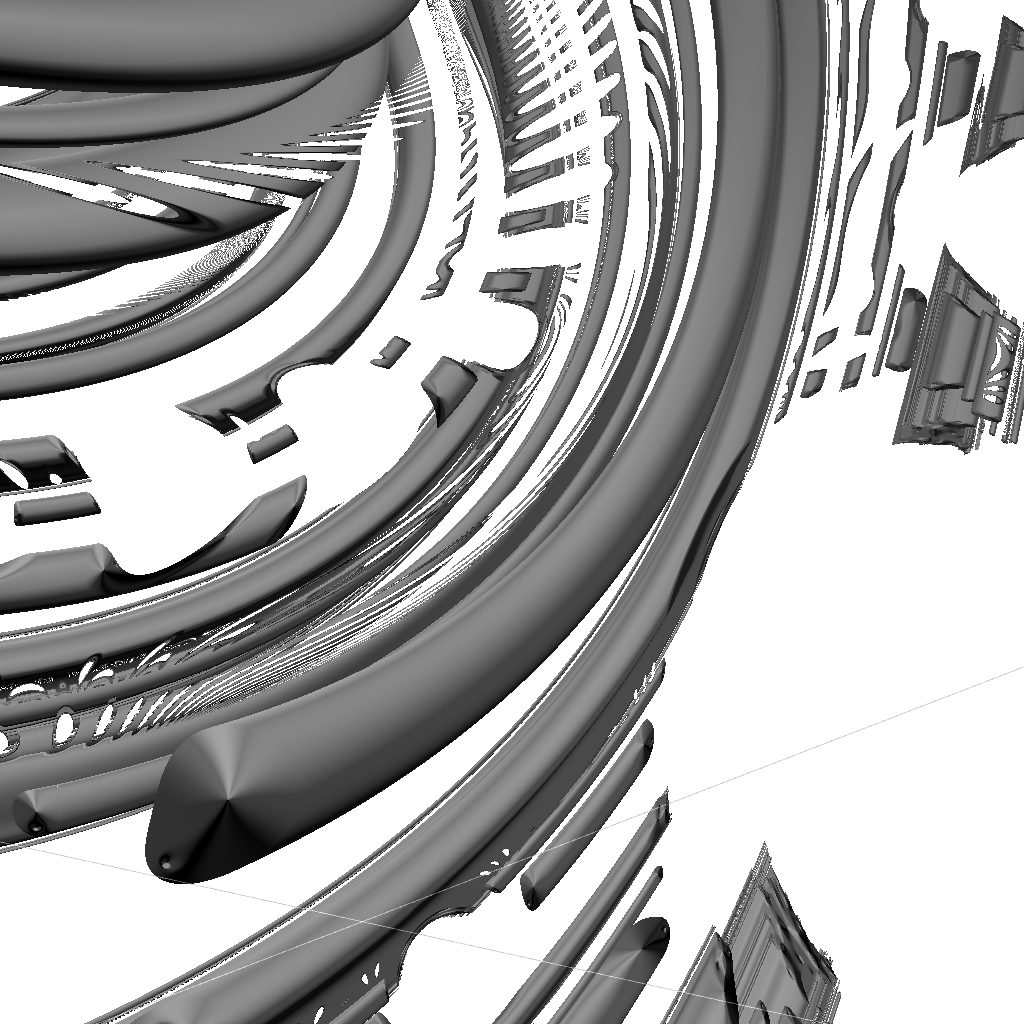
\includegraphics[width=1\linewidth]{img/julia.png}
    \caption{\label{fig:juliaRend} \it Visualization. }
    \end{subfigure} \

    \begin{subfigure}[t]{0.4\linewidth}
      \centering
      % This file was created by tikzplotlib v0.9.1.
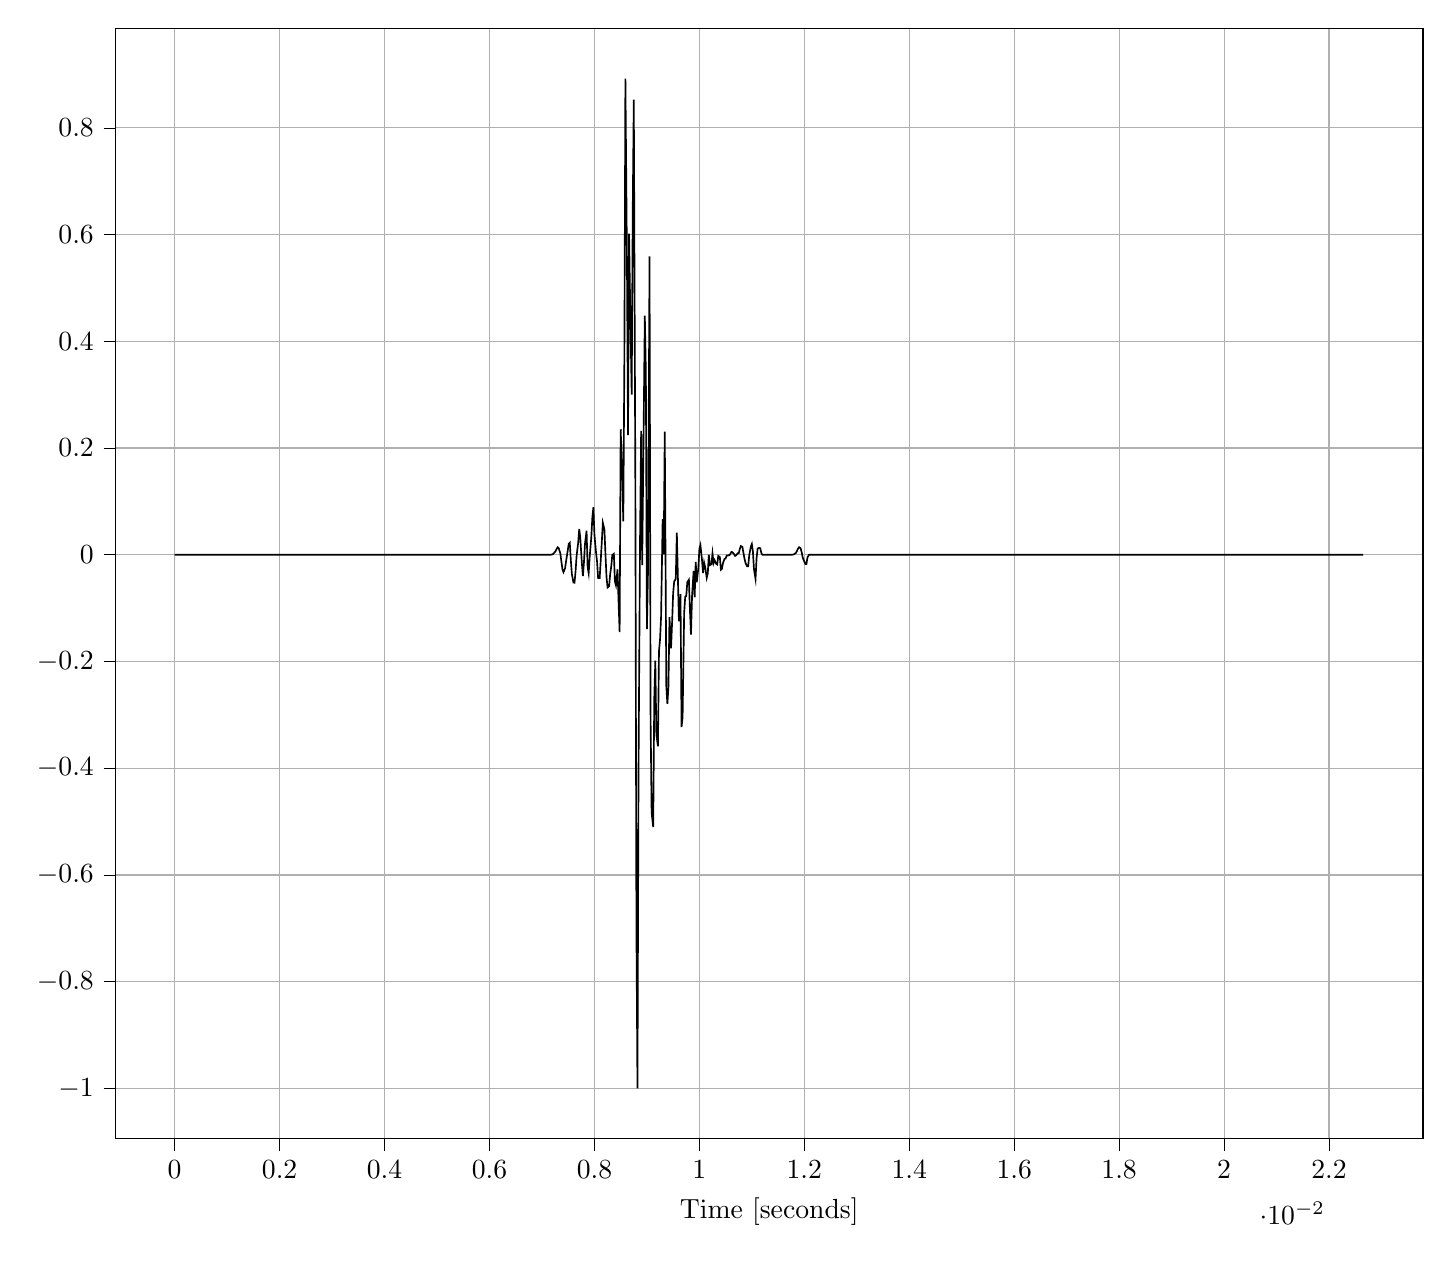
\begin{tikzpicture}

\begin{axis}[
tick align=outside,
tick pos=left,
width=1.5\textwidth,
x grid style={white!69.01961!black},
xlabel={Time [seconds]},
xmajorgrids,
xmin=-0.00113, xmax=0.02379,
xtick style={color=black},
y grid style={white!69.01961!black},
ymajorgrids,
ymin=-1.09460, ymax=0.98666,
ytick style={color=black}
]
\addplot [semithick, black]
table {%
0.00000 0.00000
0.00002 0.00000
0.00005 0.00000
0.00007 0.00000
0.00009 0.00000
0.00011 0.00000
0.00014 0.00000
0.00016 0.00000
0.00018 0.00000
0.00020 0.00000
0.00023 0.00000
0.00025 0.00000
0.00027 0.00000
0.00029 0.00000
0.00032 0.00000
0.00034 0.00000
0.00036 0.00000
0.00039 0.00000
0.00041 0.00000
0.00043 0.00000
0.00045 0.00000
0.00048 0.00000
0.00050 0.00000
0.00052 0.00000
0.00054 0.00000
0.00057 0.00000
0.00059 0.00000
0.00061 0.00000
0.00063 0.00000
0.00066 0.00000
0.00068 0.00000
0.00070 0.00000
0.00073 0.00000
0.00075 0.00000
0.00077 0.00000
0.00079 0.00000
0.00082 0.00000
0.00084 0.00000
0.00086 0.00000
0.00088 0.00000
0.00091 0.00000
0.00093 0.00000
0.00095 0.00000
0.00098 0.00000
0.00100 0.00000
0.00102 0.00000
0.00104 0.00000
0.00107 0.00000
0.00109 0.00000
0.00111 0.00000
0.00113 0.00000
0.00116 0.00000
0.00118 0.00000
0.00120 0.00000
0.00122 0.00000
0.00125 0.00000
0.00127 0.00000
0.00129 0.00000
0.00132 0.00000
0.00134 0.00000
0.00136 0.00000
0.00138 0.00000
0.00141 0.00000
0.00143 0.00000
0.00145 0.00000
0.00147 0.00000
0.00150 0.00000
0.00152 0.00000
0.00154 0.00000
0.00156 0.00000
0.00159 0.00000
0.00161 0.00000
0.00163 0.00000
0.00166 0.00000
0.00168 0.00000
0.00170 0.00000
0.00172 0.00000
0.00175 0.00000
0.00177 0.00000
0.00179 0.00000
0.00181 0.00000
0.00184 0.00000
0.00186 0.00000
0.00188 0.00000
0.00190 0.00000
0.00193 0.00000
0.00195 0.00000
0.00197 0.00000
0.00200 0.00000
0.00202 0.00000
0.00204 0.00000
0.00206 0.00000
0.00209 0.00000
0.00211 0.00000
0.00213 0.00000
0.00215 0.00000
0.00218 0.00000
0.00220 0.00000
0.00222 0.00000
0.00224 0.00000
0.00227 0.00000
0.00229 0.00000
0.00231 0.00000
0.00234 0.00000
0.00236 0.00000
0.00238 0.00000
0.00240 0.00000
0.00243 0.00000
0.00245 0.00000
0.00247 0.00000
0.00249 0.00000
0.00252 0.00000
0.00254 0.00000
0.00256 0.00000
0.00259 0.00000
0.00261 0.00000
0.00263 0.00000
0.00265 0.00000
0.00268 0.00000
0.00270 0.00000
0.00272 0.00000
0.00274 0.00000
0.00277 0.00000
0.00279 0.00000
0.00281 0.00000
0.00283 0.00000
0.00286 0.00000
0.00288 0.00000
0.00290 0.00000
0.00293 0.00000
0.00295 0.00000
0.00297 0.00000
0.00299 0.00000
0.00302 0.00000
0.00304 0.00000
0.00306 0.00000
0.00308 0.00000
0.00311 0.00000
0.00313 0.00000
0.00315 0.00000
0.00317 0.00000
0.00320 0.00000
0.00322 0.00000
0.00324 0.00000
0.00327 0.00000
0.00329 0.00000
0.00331 0.00000
0.00333 0.00000
0.00336 0.00000
0.00338 0.00000
0.00340 0.00000
0.00342 0.00000
0.00345 0.00000
0.00347 0.00000
0.00349 0.00000
0.00351 0.00000
0.00354 0.00000
0.00356 0.00000
0.00358 0.00000
0.00361 0.00000
0.00363 0.00000
0.00365 0.00000
0.00367 0.00000
0.00370 0.00000
0.00372 0.00000
0.00374 0.00000
0.00376 0.00000
0.00379 0.00000
0.00381 0.00000
0.00383 0.00000
0.00385 0.00000
0.00388 0.00000
0.00390 0.00000
0.00392 0.00000
0.00395 0.00000
0.00397 0.00000
0.00399 0.00000
0.00401 0.00000
0.00404 0.00000
0.00406 0.00000
0.00408 0.00000
0.00410 0.00000
0.00413 0.00000
0.00415 0.00000
0.00417 0.00000
0.00420 0.00000
0.00422 0.00000
0.00424 0.00000
0.00426 0.00000
0.00429 0.00000
0.00431 0.00000
0.00433 0.00000
0.00435 0.00000
0.00438 0.00000
0.00440 0.00000
0.00442 0.00000
0.00444 0.00000
0.00447 0.00000
0.00449 0.00000
0.00451 0.00000
0.00454 0.00000
0.00456 0.00000
0.00458 0.00000
0.00460 0.00000
0.00463 0.00000
0.00465 0.00000
0.00467 0.00000
0.00469 0.00000
0.00472 0.00000
0.00474 0.00000
0.00476 0.00000
0.00478 0.00000
0.00481 0.00000
0.00483 0.00000
0.00485 0.00000
0.00488 0.00000
0.00490 0.00000
0.00492 0.00000
0.00494 0.00000
0.00497 0.00000
0.00499 0.00000
0.00501 0.00000
0.00503 0.00000
0.00506 0.00000
0.00508 0.00000
0.00510 0.00000
0.00512 0.00000
0.00515 0.00000
0.00517 0.00000
0.00519 0.00000
0.00522 0.00000
0.00524 0.00000
0.00526 0.00000
0.00528 0.00000
0.00531 0.00000
0.00533 0.00000
0.00535 0.00000
0.00537 0.00000
0.00540 0.00000
0.00542 0.00000
0.00544 0.00000
0.00546 0.00000
0.00549 0.00000
0.00551 0.00000
0.00553 0.00000
0.00556 0.00000
0.00558 0.00000
0.00560 0.00000
0.00562 0.00000
0.00565 0.00000
0.00567 0.00000
0.00569 0.00000
0.00571 0.00000
0.00574 0.00000
0.00576 0.00000
0.00578 0.00000
0.00580 0.00000
0.00583 0.00000
0.00585 0.00000
0.00587 0.00000
0.00590 0.00000
0.00592 0.00000
0.00594 0.00000
0.00596 0.00000
0.00599 0.00000
0.00601 0.00000
0.00603 0.00000
0.00605 0.00000
0.00608 0.00000
0.00610 0.00000
0.00612 0.00000
0.00615 0.00000
0.00617 0.00000
0.00619 0.00000
0.00621 0.00000
0.00624 0.00000
0.00626 0.00000
0.00628 0.00000
0.00630 0.00000
0.00633 0.00000
0.00635 0.00000
0.00637 0.00000
0.00639 0.00000
0.00642 0.00000
0.00644 0.00000
0.00646 0.00000
0.00649 0.00000
0.00651 0.00000
0.00653 0.00000
0.00655 0.00000
0.00658 0.00000
0.00660 0.00000
0.00662 0.00000
0.00664 0.00000
0.00667 0.00000
0.00669 0.00000
0.00671 0.00000
0.00673 0.00000
0.00676 0.00000
0.00678 0.00000
0.00680 0.00000
0.00683 0.00000
0.00685 0.00000
0.00687 0.00000
0.00689 0.00000
0.00692 0.00000
0.00694 0.00000
0.00696 0.00000
0.00698 0.00000
0.00701 0.00000
0.00703 0.00000
0.00705 0.00000
0.00707 0.00000
0.00710 0.00000
0.00712 0.00001
0.00714 0.00004
0.00717 0.00015
0.00719 0.00051
0.00721 0.00144
0.00723 0.00343
0.00726 0.00682
0.00728 0.01105
0.00730 0.01395
0.00732 0.01202
0.00735 0.00267
0.00737 -0.01261
0.00739 -0.02713
0.00741 -0.03261
0.00744 -0.02532
0.00746 -0.01178
0.00748 0.00081
0.00751 0.02032
0.00753 0.02249
0.00755 -0.00999
0.00757 -0.03648
0.00760 -0.05201
0.00762 -0.05237
0.00764 -0.03139
0.00766 -0.00191
0.00769 0.02248
0.00771 0.04850
0.00773 0.03212
0.00776 -0.01521
0.00778 -0.03998
0.00780 -0.01425
0.00782 0.02055
0.00785 0.04505
0.00787 -0.02285
0.00789 -0.03487
0.00791 -0.00309
0.00794 0.03269
0.00796 0.06975
0.00798 0.08897
0.00800 0.03751
0.00803 0.00454
0.00805 -0.01310
0.00807 -0.04359
0.00810 -0.04351
0.00812 -0.01048
0.00814 0.02335
0.00816 0.05988
0.00819 0.04743
0.00821 0.00125
0.00823 -0.04159
0.00825 -0.06134
0.00828 -0.05857
0.00830 -0.03607
0.00832 -0.02237
0.00834 -0.00037
0.00837 0.00188
0.00839 -0.04985
0.00841 -0.05729
0.00844 -0.02727
0.00846 -0.08873
0.00848 -0.14502
0.00850 0.23515
0.00853 0.14561
0.00855 0.06252
0.00857 0.36186
0.00859 0.89206
0.00862 0.54743
0.00864 0.22412
0.00866 0.60174
0.00868 0.47177
0.00871 0.30020
0.00873 0.64694
0.00875 0.85292
0.00878 0.12483
0.00880 -0.69987
0.00882 -1.00000
0.00884 -0.40696
0.00887 0.03999
0.00889 0.23210
0.00891 -0.01939
0.00893 0.16504
0.00896 0.44807
0.00898 0.34134
0.00900 -0.13951
0.00902 -0.03473
0.00905 0.55917
0.00907 -0.30687
0.00909 -0.48376
0.00912 -0.51012
0.00914 -0.26981
0.00916 -0.19850
0.00918 -0.33667
0.00921 -0.35889
0.00923 -0.18087
0.00925 -0.15905
0.00927 -0.11629
0.00930 0.06694
0.00932 0.00068
0.00934 0.23093
0.00937 -0.24699
0.00939 -0.27953
0.00941 -0.24783
0.00943 -0.11708
0.00946 -0.17529
0.00948 -0.12682
0.00950 -0.07172
0.00952 -0.04994
0.00955 -0.04522
0.00957 0.04142
0.00959 -0.04057
0.00961 -0.12491
0.00964 -0.07397
0.00966 -0.32289
0.00968 -0.30482
0.00971 -0.10805
0.00973 -0.07891
0.00975 -0.07692
0.00977 -0.05111
0.00980 -0.04666
0.00982 -0.10372
0.00984 -0.14943
0.00986 -0.07767
0.00989 -0.03045
0.00991 -0.07958
0.00993 -0.01334
0.00995 -0.05169
0.00998 -0.02477
0.01000 0.01105
0.01002 0.01813
0.01005 -0.00980
0.01007 -0.03430
0.01009 -0.01453
0.01011 -0.02276
0.01014 -0.04334
0.01016 -0.03501
0.01018 0.00006
0.01020 -0.01945
0.01023 -0.01771
0.01025 0.00249
0.01027 -0.01579
0.01029 -0.01021
0.01032 -0.01698
0.01034 -0.01830
0.01036 -0.00217
0.01039 -0.00423
0.01041 -0.02795
0.01043 -0.02601
0.01045 -0.01544
0.01048 -0.00745
0.01050 -0.00705
0.01052 -0.00122
0.01054 -0.00139
0.01057 -0.00075
0.01059 0.00155
0.01061 0.00540
0.01063 0.00472
0.01066 0.00130
0.01068 -0.00218
0.01070 -0.00103
0.01073 0.00286
0.01075 0.00269
0.01077 0.01063
0.01079 0.01634
0.01082 0.01460
0.01084 0.00342
0.01086 -0.00734
0.01088 -0.01554
0.01091 -0.02164
0.01093 -0.02152
0.01095 -0.00087
0.01098 0.01503
0.01100 0.02022
0.01102 0.00612
0.01104 -0.02690
0.01107 -0.04540
0.01109 -0.00655
0.01111 0.01167
0.01113 0.01274
0.01116 0.01244
0.01118 0.00356
0.01120 0.00000
0.01122 0.00000
0.01125 0.00000
0.01127 0.00000
0.01129 0.00000
0.01132 0.00000
0.01134 0.00000
0.01136 0.00000
0.01138 0.00000
0.01141 0.00000
0.01143 0.00000
0.01145 0.00000
0.01147 0.00000
0.01150 0.00000
0.01152 0.00000
0.01154 0.00000
0.01156 0.00000
0.01159 0.00000
0.01161 0.00000
0.01163 0.00000
0.01166 0.00000
0.01168 0.00000
0.01170 0.00000
0.01172 0.00000
0.01175 0.00002
0.01177 0.00011
0.01179 0.00044
0.01181 0.00137
0.01184 0.00348
0.01186 0.00712
0.01188 0.01149
0.01190 0.01414
0.01193 0.01205
0.01195 0.00447
0.01197 -0.00555
0.01200 -0.01296
0.01202 -0.01717
0.01204 -0.01722
0.01206 -0.00491
0.01209 0.00000
0.01211 0.00000
0.01213 0.00000
0.01215 0.00000
0.01218 0.00000
0.01220 0.00000
0.01222 0.00000
0.01224 0.00000
0.01227 0.00000
0.01229 0.00000
0.01231 0.00000
0.01234 0.00000
0.01236 0.00000
0.01238 0.00000
0.01240 0.00000
0.01243 0.00000
0.01245 0.00000
0.01247 0.00000
0.01249 0.00000
0.01252 0.00000
0.01254 0.00000
0.01256 0.00000
0.01259 0.00000
0.01261 0.00000
0.01263 0.00000
0.01265 0.00000
0.01268 0.00000
0.01270 0.00000
0.01272 0.00000
0.01274 0.00000
0.01277 0.00000
0.01279 0.00000
0.01281 0.00000
0.01283 0.00000
0.01286 0.00000
0.01288 0.00000
0.01290 0.00000
0.01293 0.00000
0.01295 0.00000
0.01297 0.00000
0.01299 0.00000
0.01302 0.00000
0.01304 0.00000
0.01306 0.00000
0.01308 0.00000
0.01311 0.00000
0.01313 0.00000
0.01315 0.00000
0.01317 0.00000
0.01320 0.00000
0.01322 0.00000
0.01324 0.00000
0.01327 0.00000
0.01329 0.00000
0.01331 0.00000
0.01333 0.00000
0.01336 0.00000
0.01338 0.00000
0.01340 0.00000
0.01342 0.00000
0.01345 0.00000
0.01347 0.00000
0.01349 0.00000
0.01351 0.00000
0.01354 0.00000
0.01356 0.00000
0.01358 0.00000
0.01361 0.00000
0.01363 0.00000
0.01365 0.00000
0.01367 0.00000
0.01370 0.00000
0.01372 0.00000
0.01374 0.00000
0.01376 0.00000
0.01379 0.00000
0.01381 0.00000
0.01383 0.00000
0.01385 0.00000
0.01388 0.00000
0.01390 0.00000
0.01392 0.00000
0.01395 0.00000
0.01397 0.00000
0.01399 0.00000
0.01401 0.00000
0.01404 0.00000
0.01406 0.00000
0.01408 0.00000
0.01410 0.00000
0.01413 0.00000
0.01415 0.00000
0.01417 0.00000
0.01420 0.00000
0.01422 0.00000
0.01424 0.00000
0.01426 0.00000
0.01429 0.00000
0.01431 0.00000
0.01433 0.00000
0.01435 0.00000
0.01438 0.00000
0.01440 0.00000
0.01442 0.00000
0.01444 0.00000
0.01447 0.00000
0.01449 0.00000
0.01451 0.00000
0.01454 0.00000
0.01456 0.00000
0.01458 0.00000
0.01460 0.00000
0.01463 0.00000
0.01465 0.00000
0.01467 0.00000
0.01469 0.00000
0.01472 0.00000
0.01474 0.00000
0.01476 0.00000
0.01478 0.00000
0.01481 0.00000
0.01483 0.00000
0.01485 0.00000
0.01488 0.00000
0.01490 0.00000
0.01492 0.00000
0.01494 0.00000
0.01497 0.00000
0.01499 0.00000
0.01501 0.00000
0.01503 0.00000
0.01506 0.00000
0.01508 0.00000
0.01510 0.00000
0.01512 0.00000
0.01515 0.00000
0.01517 0.00000
0.01519 0.00000
0.01522 0.00000
0.01524 0.00000
0.01526 0.00000
0.01528 0.00000
0.01531 0.00000
0.01533 0.00000
0.01535 0.00000
0.01537 0.00000
0.01540 0.00000
0.01542 0.00000
0.01544 0.00000
0.01546 0.00000
0.01549 0.00000
0.01551 0.00000
0.01553 0.00000
0.01556 0.00000
0.01558 0.00000
0.01560 0.00000
0.01562 0.00000
0.01565 0.00000
0.01567 0.00000
0.01569 0.00000
0.01571 0.00000
0.01574 0.00000
0.01576 0.00000
0.01578 0.00000
0.01580 0.00000
0.01583 0.00000
0.01585 0.00000
0.01587 0.00000
0.01590 0.00000
0.01592 0.00000
0.01594 0.00000
0.01596 0.00000
0.01599 0.00000
0.01601 0.00000
0.01603 0.00000
0.01605 0.00000
0.01608 0.00000
0.01610 0.00000
0.01612 0.00000
0.01615 0.00000
0.01617 0.00000
0.01619 0.00000
0.01621 0.00000
0.01624 0.00000
0.01626 0.00000
0.01628 0.00000
0.01630 0.00000
0.01633 0.00000
0.01635 0.00000
0.01637 0.00000
0.01639 0.00000
0.01642 0.00000
0.01644 0.00000
0.01646 0.00000
0.01649 0.00000
0.01651 0.00000
0.01653 0.00000
0.01655 0.00000
0.01658 0.00000
0.01660 0.00000
0.01662 0.00000
0.01664 0.00000
0.01667 0.00000
0.01669 0.00000
0.01671 0.00000
0.01673 0.00000
0.01676 0.00000
0.01678 0.00000
0.01680 0.00000
0.01683 0.00000
0.01685 0.00000
0.01687 0.00000
0.01689 0.00000
0.01692 0.00000
0.01694 0.00000
0.01696 0.00000
0.01698 0.00000
0.01701 0.00000
0.01703 0.00000
0.01705 0.00000
0.01707 0.00000
0.01710 0.00000
0.01712 0.00000
0.01714 0.00000
0.01717 0.00000
0.01719 0.00000
0.01721 0.00000
0.01723 0.00000
0.01726 0.00000
0.01728 0.00000
0.01730 0.00000
0.01732 0.00000
0.01735 0.00000
0.01737 0.00000
0.01739 0.00000
0.01741 0.00000
0.01744 0.00000
0.01746 0.00000
0.01748 0.00000
0.01751 0.00000
0.01753 0.00000
0.01755 0.00000
0.01757 0.00000
0.01760 0.00000
0.01762 0.00000
0.01764 0.00000
0.01766 0.00000
0.01769 0.00000
0.01771 0.00000
0.01773 0.00000
0.01776 0.00000
0.01778 0.00000
0.01780 0.00000
0.01782 0.00000
0.01785 0.00000
0.01787 0.00000
0.01789 0.00000
0.01791 0.00000
0.01794 0.00000
0.01796 0.00000
0.01798 0.00000
0.01800 0.00000
0.01803 0.00000
0.01805 0.00000
0.01807 0.00000
0.01810 0.00000
0.01812 0.00000
0.01814 0.00000
0.01816 0.00000
0.01819 0.00000
0.01821 0.00000
0.01823 0.00000
0.01825 0.00000
0.01828 0.00000
0.01830 0.00000
0.01832 0.00000
0.01834 0.00000
0.01837 0.00000
0.01839 0.00000
0.01841 0.00000
0.01844 0.00000
0.01846 0.00000
0.01848 0.00000
0.01850 0.00000
0.01853 0.00000
0.01855 0.00000
0.01857 0.00000
0.01859 0.00000
0.01862 0.00000
0.01864 0.00000
0.01866 0.00000
0.01868 0.00000
0.01871 0.00000
0.01873 0.00000
0.01875 0.00000
0.01878 0.00000
0.01880 0.00000
0.01882 0.00000
0.01884 0.00000
0.01887 0.00000
0.01889 0.00000
0.01891 0.00000
0.01893 0.00000
0.01896 0.00000
0.01898 0.00000
0.01900 0.00000
0.01902 0.00000
0.01905 0.00000
0.01907 0.00000
0.01909 0.00000
0.01912 0.00000
0.01914 0.00000
0.01916 0.00000
0.01918 0.00000
0.01921 0.00000
0.01923 0.00000
0.01925 0.00000
0.01927 0.00000
0.01930 0.00000
0.01932 0.00000
0.01934 0.00000
0.01937 0.00000
0.01939 0.00000
0.01941 0.00000
0.01943 0.00000
0.01946 0.00000
0.01948 0.00000
0.01950 0.00000
0.01952 0.00000
0.01955 0.00000
0.01957 0.00000
0.01959 0.00000
0.01961 0.00000
0.01964 0.00000
0.01966 0.00000
0.01968 0.00000
0.01971 0.00000
0.01973 0.00000
0.01975 0.00000
0.01977 0.00000
0.01980 0.00000
0.01982 0.00000
0.01984 0.00000
0.01986 0.00000
0.01989 0.00000
0.01991 0.00000
0.01993 0.00000
0.01995 0.00000
0.01998 0.00000
0.02000 0.00000
0.02002 0.00000
0.02005 0.00000
0.02007 0.00000
0.02009 0.00000
0.02011 0.00000
0.02014 0.00000
0.02016 0.00000
0.02018 0.00000
0.02020 0.00000
0.02023 0.00000
0.02025 0.00000
0.02027 0.00000
0.02029 0.00000
0.02032 0.00000
0.02034 0.00000
0.02036 0.00000
0.02039 0.00000
0.02041 0.00000
0.02043 0.00000
0.02045 0.00000
0.02048 0.00000
0.02050 0.00000
0.02052 0.00000
0.02054 0.00000
0.02057 0.00000
0.02059 0.00000
0.02061 0.00000
0.02063 0.00000
0.02066 0.00000
0.02068 0.00000
0.02070 0.00000
0.02073 0.00000
0.02075 0.00000
0.02077 0.00000
0.02079 0.00000
0.02082 0.00000
0.02084 0.00000
0.02086 0.00000
0.02088 0.00000
0.02091 0.00000
0.02093 0.00000
0.02095 0.00000
0.02098 0.00000
0.02100 0.00000
0.02102 0.00000
0.02104 0.00000
0.02107 0.00000
0.02109 0.00000
0.02111 0.00000
0.02113 0.00000
0.02116 0.00000
0.02118 0.00000
0.02120 0.00000
0.02122 0.00000
0.02125 0.00000
0.02127 0.00000
0.02129 0.00000
0.02132 0.00000
0.02134 0.00000
0.02136 0.00000
0.02138 0.00000
0.02141 0.00000
0.02143 0.00000
0.02145 0.00000
0.02147 0.00000
0.02150 0.00000
0.02152 0.00000
0.02154 0.00000
0.02156 0.00000
0.02159 0.00000
0.02161 0.00000
0.02163 0.00000
0.02166 0.00000
0.02168 0.00000
0.02170 0.00000
0.02172 0.00000
0.02175 0.00000
0.02177 0.00000
0.02179 0.00000
0.02181 0.00000
0.02184 0.00000
0.02186 0.00000
0.02188 0.00000
0.02190 0.00000
0.02193 0.00000
0.02195 0.00000
0.02197 0.00000
0.02200 0.00000
0.02202 0.00000
0.02204 0.00000
0.02206 0.00000
0.02209 0.00000
0.02211 0.00000
0.02213 0.00000
0.02215 0.00000
0.02218 0.00000
0.02220 0.00000
0.02222 0.00000
0.02224 0.00000
0.02227 0.00000
0.02229 0.00000
0.02231 0.00000
0.02234 0.00000
0.02236 0.00000
0.02238 0.00000
0.02240 0.00000
0.02243 0.00000
0.02245 0.00000
0.02247 0.00000
0.02249 0.00000
0.02252 0.00000
0.02254 0.00000
0.02256 0.00000
0.02259 0.00000
0.02261 0.00000
0.02263 0.00000
0.02265 0.00000
};
\end{axis}

\end{tikzpicture}

      \caption{\label{fig:juliaRIR} \it RIR simulated using the proposed method. }
    \end{subfigure}
    \caption{\it Visualization (a) and RIR (b) of a 3-dimensional projection of a 4-dimensional function, the Julia Set \cite{quilez_inigo_nodate-1} .}
    \label{fig:julia}
\end{figure}



% Please, submit full-length papers (max.~8 pages both oral and poster presentations).
% Submission is fully electronic and automated through the Conference Web Submission System.
% DO NOT send us papers directly by e-mail.

% \section{Acknowledgments}
% This work was supported in part by the university of Applied sciences St.Poelten.
% Thanks to inigo quilez, the shadertoy community.
% Many thanks to the great number of anonymous reviewers!

%\newpage
\nocite{*}
\bibliographystyle{IEEEbib}
\bibliography{RaymarchReverb2}


\end{document}





% \begin{figure}
%     \begin{center}
%       % This file was created by tikzplotlib v0.9.1.
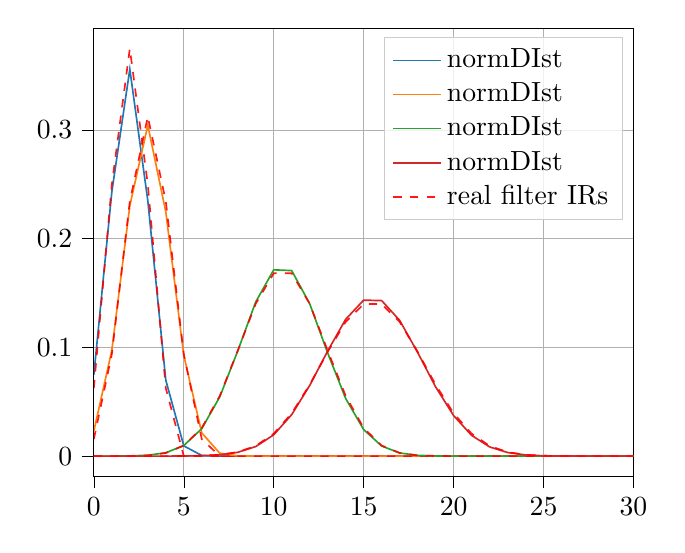
\begin{tikzpicture}

\definecolor{color0}{rgb}{0.1216,0.4667,0.7059}
\definecolor{color1}{rgb}{1.0000,0.4980,0.0549}
\definecolor{color2}{rgb}{0.1725,0.6275,0.1725}
\definecolor{color3}{rgb}{0.8392,0.1529,0.1569}

\begin{axis}[
legend cell align={left},
legend style={fill opacity=0.8, draw opacity=1, text opacity=1, draw=white!80.0000!black},
tick align=outside,
tick pos=left,
x grid style={white!69.0196!black},
xmajorgrids,
xmin=0.0000, xmax=30.0000,
xtick style={color=black},
y grid style={white!69.0196!black},
ymajorgrids,
ymin=-0.0188, ymax=0.3937,
ytick style={color=black}
]
\addplot [semithick, color0]
table {%
0.0000 0.0749
1.0000 0.2432
2.0000 0.3560
3.0000 0.2350
4.0000 0.0699
5.0000 0.0094
6.0000 0.0006
7.0000 0.0000
8.0000 0.0000
9.0000 0.0000
10.0000 0.0000
11.0000 0.0000
12.0000 0.0000
13.0000 0.0000
14.0000 0.0000
15.0000 0.0000
16.0000 0.0000
17.0000 0.0000
18.0000 0.0000
19.0000 0.0000
20.0000 0.0000
21.0000 0.0000
22.0000 0.0000
23.0000 0.0000
24.0000 0.0000
25.0000 0.0000
26.0000 0.0000
27.0000 0.0000
28.0000 0.0000
29.0000 0.0000
30.0000 0.0000
31.0000 0.0000
32.0000 0.0000
33.0000 0.0000
34.0000 0.0000
35.0000 0.0000
36.0000 0.0000
37.0000 0.0000
38.0000 0.0000
39.0000 0.0000
40.0000 0.0000
41.0000 0.0000
42.0000 0.0000
43.0000 0.0000
44.0000 0.0000
45.0000 0.0000
46.0000 0.0000
47.0000 0.0000
48.0000 0.0000
49.0000 0.0000
50.0000 0.0000
51.0000 0.0000
52.0000 0.0000
53.0000 0.0000
54.0000 0.0000
55.0000 0.0000
56.0000 0.0000
57.0000 0.0000
58.0000 0.0000
59.0000 0.0000
60.0000 0.0000
61.0000 0.0000
62.0000 0.0000
63.0000 0.0000
64.0000 0.0000
65.0000 0.0000
66.0000 0.0000
67.0000 0.0000
68.0000 0.0000
69.0000 0.0000
70.0000 0.0000
71.0000 0.0000
72.0000 0.0000
73.0000 0.0000
74.0000 0.0000
75.0000 0.0000
76.0000 0.0000
77.0000 0.0000
78.0000 0.0000
79.0000 0.0000
80.0000 0.0000
81.0000 0.0000
82.0000 0.0000
83.0000 0.0000
84.0000 0.0000
85.0000 0.0000
86.0000 0.0000
87.0000 0.0000
88.0000 0.0000
89.0000 0.0000
90.0000 0.0000
91.0000 0.0000
92.0000 0.0000
93.0000 0.0000
94.0000 0.0000
95.0000 0.0000
96.0000 0.0000
97.0000 0.0000
98.0000 0.0000
99.0000 0.0000
};
\addlegendentry{normDIst}
\addplot [semithick, red, opacity=0.9, dashed, forget plot]
table {%
0.0000 0.0625
1.0000 0.2500
2.0000 0.3750
3.0000 0.2500
4.0000 0.0625
5.0000 0.0000
6.0000 0.0000
7.0000 0.0000
8.0000 0.0000
9.0000 0.0000
10.0000 0.0000
11.0000 0.0000
12.0000 0.0000
13.0000 0.0000
14.0000 0.0000
15.0000 0.0000
16.0000 0.0000
17.0000 0.0000
18.0000 0.0000
19.0000 0.0000
20.0000 0.0000
21.0000 0.0000
22.0000 0.0000
23.0000 0.0000
24.0000 0.0000
25.0000 0.0000
26.0000 0.0000
27.0000 0.0000
28.0000 0.0000
29.0000 0.0000
30.0000 0.0000
31.0000 0.0000
32.0000 0.0000
33.0000 0.0000
34.0000 0.0000
35.0000 0.0000
36.0000 0.0000
37.0000 0.0000
38.0000 0.0000
39.0000 0.0000
40.0000 0.0000
41.0000 0.0000
42.0000 0.0000
43.0000 0.0000
44.0000 0.0000
45.0000 0.0000
46.0000 0.0000
47.0000 0.0000
48.0000 0.0000
49.0000 0.0000
50.0000 0.0000
51.0000 0.0000
52.0000 0.0000
53.0000 0.0000
54.0000 0.0000
55.0000 0.0000
56.0000 0.0000
57.0000 0.0000
58.0000 0.0000
59.0000 0.0000
60.0000 0.0000
61.0000 0.0000
62.0000 0.0000
63.0000 0.0000
64.0000 0.0000
65.0000 0.0000
66.0000 0.0000
67.0000 0.0000
68.0000 0.0000
69.0000 0.0000
70.0000 0.0000
71.0000 0.0000
72.0000 0.0000
73.0000 0.0000
74.0000 0.0000
75.0000 0.0000
76.0000 0.0000
77.0000 0.0000
78.0000 0.0000
79.0000 0.0000
80.0000 0.0000
81.0000 0.0000
82.0000 0.0000
83.0000 0.0000
84.0000 0.0000
85.0000 0.0000
86.0000 0.0000
87.0000 0.0000
88.0000 0.0000
89.0000 0.0000
90.0000 0.0000
91.0000 0.0000
92.0000 0.0000
93.0000 0.0000
94.0000 0.0000
95.0000 0.0000
96.0000 0.0000
97.0000 0.0000
98.0000 0.0000
99.0000 0.0000
};
\addplot [semithick, color1]
table {%
0.0000 0.0230
1.0000 0.0974
2.0000 0.2304
3.0000 0.3044
4.0000 0.2247
5.0000 0.0926
6.0000 0.0213
7.0000 0.0027
8.0000 0.0002
9.0000 0.0000
10.0000 0.0000
11.0000 0.0000
12.0000 0.0000
13.0000 0.0000
14.0000 0.0000
15.0000 0.0000
16.0000 0.0000
17.0000 0.0000
18.0000 0.0000
19.0000 0.0000
20.0000 0.0000
21.0000 0.0000
22.0000 0.0000
23.0000 0.0000
24.0000 0.0000
25.0000 0.0000
26.0000 0.0000
27.0000 0.0000
28.0000 0.0000
29.0000 0.0000
30.0000 0.0000
31.0000 0.0000
32.0000 0.0000
33.0000 0.0000
34.0000 0.0000
35.0000 0.0000
36.0000 0.0000
37.0000 0.0000
38.0000 0.0000
39.0000 0.0000
40.0000 0.0000
41.0000 0.0000
42.0000 0.0000
43.0000 0.0000
44.0000 0.0000
45.0000 0.0000
46.0000 0.0000
47.0000 0.0000
48.0000 0.0000
49.0000 0.0000
50.0000 0.0000
51.0000 0.0000
52.0000 0.0000
53.0000 0.0000
54.0000 0.0000
55.0000 0.0000
56.0000 0.0000
57.0000 0.0000
58.0000 0.0000
59.0000 0.0000
60.0000 0.0000
61.0000 0.0000
62.0000 0.0000
63.0000 0.0000
64.0000 0.0000
65.0000 0.0000
66.0000 0.0000
67.0000 0.0000
68.0000 0.0000
69.0000 0.0000
70.0000 0.0000
71.0000 0.0000
72.0000 0.0000
73.0000 0.0000
74.0000 0.0000
75.0000 0.0000
76.0000 0.0000
77.0000 0.0000
78.0000 0.0000
79.0000 0.0000
80.0000 0.0000
81.0000 0.0000
82.0000 0.0000
83.0000 0.0000
84.0000 0.0000
85.0000 0.0000
86.0000 0.0000
87.0000 0.0000
88.0000 0.0000
89.0000 0.0000
90.0000 0.0000
91.0000 0.0000
92.0000 0.0000
93.0000 0.0000
94.0000 0.0000
95.0000 0.0000
96.0000 0.0000
97.0000 0.0000
98.0000 0.0000
99.0000 0.0000
};
\addlegendentry{normDIst}
\addplot [semithick, red, opacity=0.9, dashed, forget plot]
table {%
0.0000 0.0156
1.0000 0.0938
2.0000 0.2344
3.0000 0.3125
4.0000 0.2344
5.0000 0.0938
6.0000 0.0156
7.0000 0.0000
8.0000 0.0000
9.0000 0.0000
10.0000 0.0000
11.0000 0.0000
12.0000 0.0000
13.0000 0.0000
14.0000 0.0000
15.0000 0.0000
16.0000 0.0000
17.0000 0.0000
18.0000 0.0000
19.0000 0.0000
20.0000 0.0000
21.0000 0.0000
22.0000 0.0000
23.0000 0.0000
24.0000 0.0000
25.0000 0.0000
26.0000 0.0000
27.0000 0.0000
28.0000 0.0000
29.0000 0.0000
30.0000 0.0000
31.0000 0.0000
32.0000 0.0000
33.0000 0.0000
34.0000 0.0000
35.0000 0.0000
36.0000 0.0000
37.0000 0.0000
38.0000 0.0000
39.0000 0.0000
40.0000 0.0000
41.0000 0.0000
42.0000 0.0000
43.0000 0.0000
44.0000 0.0000
45.0000 0.0000
46.0000 0.0000
47.0000 0.0000
48.0000 0.0000
49.0000 0.0000
50.0000 0.0000
51.0000 0.0000
52.0000 0.0000
53.0000 0.0000
54.0000 0.0000
55.0000 0.0000
56.0000 0.0000
57.0000 0.0000
58.0000 0.0000
59.0000 0.0000
60.0000 0.0000
61.0000 0.0000
62.0000 0.0000
63.0000 0.0000
64.0000 0.0000
65.0000 0.0000
66.0000 0.0000
67.0000 0.0000
68.0000 0.0000
69.0000 0.0000
70.0000 0.0000
71.0000 0.0000
72.0000 0.0000
73.0000 0.0000
74.0000 0.0000
75.0000 0.0000
76.0000 0.0000
77.0000 0.0000
78.0000 0.0000
79.0000 0.0000
80.0000 0.0000
81.0000 0.0000
82.0000 0.0000
83.0000 0.0000
84.0000 0.0000
85.0000 0.0000
86.0000 0.0000
87.0000 0.0000
88.0000 0.0000
89.0000 0.0000
90.0000 0.0000
91.0000 0.0000
92.0000 0.0000
93.0000 0.0000
94.0000 0.0000
95.0000 0.0000
96.0000 0.0000
97.0000 0.0000
98.0000 0.0000
99.0000 0.0000
};
\addplot [semithick, color2]
table {%
0.0000 0.0000
1.0000 0.0000
2.0000 0.0002
3.0000 0.0008
4.0000 0.0031
5.0000 0.0097
6.0000 0.0253
7.0000 0.0545
8.0000 0.0968
9.0000 0.1419
10.0000 0.1714
11.0000 0.1707
12.0000 0.1402
13.0000 0.0949
14.0000 0.0530
15.0000 0.0244
16.0000 0.0093
17.0000 0.0029
18.0000 0.0007
19.0000 0.0002
20.0000 0.0000
21.0000 0.0000
22.0000 0.0000
23.0000 0.0000
24.0000 0.0000
25.0000 0.0000
26.0000 0.0000
27.0000 0.0000
28.0000 0.0000
29.0000 0.0000
30.0000 0.0000
31.0000 0.0000
32.0000 0.0000
33.0000 0.0000
34.0000 0.0000
35.0000 0.0000
36.0000 0.0000
37.0000 0.0000
38.0000 0.0000
39.0000 0.0000
40.0000 0.0000
41.0000 0.0000
42.0000 0.0000
43.0000 0.0000
44.0000 0.0000
45.0000 0.0000
46.0000 0.0000
47.0000 0.0000
48.0000 0.0000
49.0000 0.0000
50.0000 0.0000
51.0000 0.0000
52.0000 0.0000
53.0000 0.0000
54.0000 0.0000
55.0000 0.0000
56.0000 0.0000
57.0000 0.0000
58.0000 0.0000
59.0000 0.0000
60.0000 0.0000
61.0000 0.0000
62.0000 0.0000
63.0000 0.0000
64.0000 0.0000
65.0000 0.0000
66.0000 0.0000
67.0000 0.0000
68.0000 0.0000
69.0000 0.0000
70.0000 0.0000
71.0000 0.0000
72.0000 0.0000
73.0000 0.0000
74.0000 0.0000
75.0000 0.0000
76.0000 0.0000
77.0000 0.0000
78.0000 0.0000
79.0000 0.0000
80.0000 0.0000
81.0000 0.0000
82.0000 0.0000
83.0000 0.0000
84.0000 0.0000
85.0000 0.0000
86.0000 0.0000
87.0000 0.0000
88.0000 0.0000
89.0000 0.0000
90.0000 0.0000
91.0000 0.0000
92.0000 0.0000
93.0000 0.0000
94.0000 0.0000
95.0000 0.0000
96.0000 0.0000
97.0000 0.0000
98.0000 0.0000
99.0000 0.0000
};
\addlegendentry{normDIst}
\addplot [semithick, red, opacity=0.9, dashed, forget plot]
table {%
0.0000 0.0000
1.0000 0.0000
2.0000 0.0001
3.0000 0.0006
4.0000 0.0029
5.0000 0.0097
6.0000 0.0259
7.0000 0.0554
8.0000 0.0970
9.0000 0.1402
10.0000 0.1682
11.0000 0.1682
12.0000 0.1402
13.0000 0.0970
14.0000 0.0554
15.0000 0.0259
16.0000 0.0097
17.0000 0.0029
18.0000 0.0006
19.0000 0.0001
20.0000 0.0000
21.0000 0.0000
22.0000 0.0000
23.0000 0.0000
24.0000 0.0000
25.0000 0.0000
26.0000 0.0000
27.0000 0.0000
28.0000 0.0000
29.0000 0.0000
30.0000 0.0000
31.0000 0.0000
32.0000 0.0000
33.0000 0.0000
34.0000 0.0000
35.0000 0.0000
36.0000 0.0000
37.0000 0.0000
38.0000 0.0000
39.0000 0.0000
40.0000 0.0000
41.0000 0.0000
42.0000 0.0000
43.0000 0.0000
44.0000 0.0000
45.0000 0.0000
46.0000 0.0000
47.0000 0.0000
48.0000 0.0000
49.0000 0.0000
50.0000 0.0000
51.0000 0.0000
52.0000 0.0000
53.0000 0.0000
54.0000 0.0000
55.0000 0.0000
56.0000 0.0000
57.0000 0.0000
58.0000 0.0000
59.0000 0.0000
60.0000 0.0000
61.0000 0.0000
62.0000 0.0000
63.0000 0.0000
64.0000 0.0000
65.0000 0.0000
66.0000 0.0000
67.0000 0.0000
68.0000 0.0000
69.0000 0.0000
70.0000 0.0000
71.0000 0.0000
72.0000 0.0000
73.0000 0.0000
74.0000 0.0000
75.0000 0.0000
76.0000 0.0000
77.0000 0.0000
78.0000 0.0000
79.0000 0.0000
80.0000 0.0000
81.0000 0.0000
82.0000 0.0000
83.0000 0.0000
84.0000 0.0000
85.0000 0.0000
86.0000 0.0000
87.0000 0.0000
88.0000 0.0000
89.0000 0.0000
90.0000 0.0000
91.0000 0.0000
92.0000 0.0000
93.0000 0.0000
94.0000 0.0000
95.0000 0.0000
96.0000 0.0000
97.0000 0.0000
98.0000 0.0000
99.0000 0.0000
};
\addplot [semithick, color3]
table {%
0.0000 0.0000
1.0000 0.0000
2.0000 0.0000
3.0000 0.0000
4.0000 0.0000
5.0000 0.0001
6.0000 0.0004
7.0000 0.0012
8.0000 0.0035
9.0000 0.0088
10.0000 0.0196
11.0000 0.0382
12.0000 0.0650
13.0000 0.0967
14.0000 0.1259
15.0000 0.1435
16.0000 0.1431
17.0000 0.1249
18.0000 0.0954
19.0000 0.0637
20.0000 0.0373
21.0000 0.0191
22.0000 0.0085
23.0000 0.0033
24.0000 0.0011
25.0000 0.0003
26.0000 0.0001
27.0000 0.0000
28.0000 0.0000
29.0000 0.0000
30.0000 0.0000
31.0000 0.0000
32.0000 0.0000
33.0000 0.0000
34.0000 0.0000
35.0000 0.0000
36.0000 0.0000
37.0000 0.0000
38.0000 0.0000
39.0000 0.0000
40.0000 0.0000
41.0000 0.0000
42.0000 0.0000
43.0000 0.0000
44.0000 0.0000
45.0000 0.0000
46.0000 0.0000
47.0000 0.0000
48.0000 0.0000
49.0000 0.0000
50.0000 0.0000
51.0000 0.0000
52.0000 0.0000
53.0000 0.0000
54.0000 0.0000
55.0000 0.0000
56.0000 0.0000
57.0000 0.0000
58.0000 0.0000
59.0000 0.0000
60.0000 0.0000
61.0000 0.0000
62.0000 0.0000
63.0000 0.0000
64.0000 0.0000
65.0000 0.0000
66.0000 0.0000
67.0000 0.0000
68.0000 0.0000
69.0000 0.0000
70.0000 0.0000
71.0000 0.0000
72.0000 0.0000
73.0000 0.0000
74.0000 0.0000
75.0000 0.0000
76.0000 0.0000
77.0000 0.0000
78.0000 0.0000
79.0000 0.0000
80.0000 0.0000
81.0000 0.0000
82.0000 0.0000
83.0000 0.0000
84.0000 0.0000
85.0000 0.0000
86.0000 0.0000
87.0000 0.0000
88.0000 0.0000
89.0000 0.0000
90.0000 0.0000
91.0000 0.0000
92.0000 0.0000
93.0000 0.0000
94.0000 0.0000
95.0000 0.0000
96.0000 0.0000
97.0000 0.0000
98.0000 0.0000
99.0000 0.0000
};
\addlegendentry{normDIst}
\addplot [semithick, red, opacity=0.9, dashed]
table {%
0.0000 0.0000
1.0000 0.0000
2.0000 0.0000
3.0000 0.0000
4.0000 0.0000
5.0000 0.0001
6.0000 0.0003
7.0000 0.0012
8.0000 0.0037
9.0000 0.0094
10.0000 0.0207
11.0000 0.0394
12.0000 0.0657
13.0000 0.0960
14.0000 0.1235
15.0000 0.1399
16.0000 0.1399
17.0000 0.1235
18.0000 0.0960
19.0000 0.0657
20.0000 0.0394
21.0000 0.0207
22.0000 0.0094
23.0000 0.0037
24.0000 0.0012
25.0000 0.0003
26.0000 0.0001
27.0000 0.0000
28.0000 0.0000
29.0000 0.0000
30.0000 0.0000
31.0000 0.0000
32.0000 0.0000
33.0000 0.0000
34.0000 0.0000
35.0000 0.0000
36.0000 0.0000
37.0000 0.0000
38.0000 0.0000
39.0000 0.0000
40.0000 0.0000
41.0000 0.0000
42.0000 0.0000
43.0000 0.0000
44.0000 0.0000
45.0000 0.0000
46.0000 0.0000
47.0000 0.0000
48.0000 0.0000
49.0000 0.0000
50.0000 0.0000
51.0000 0.0000
52.0000 0.0000
53.0000 0.0000
54.0000 0.0000
55.0000 0.0000
56.0000 0.0000
57.0000 0.0000
58.0000 0.0000
59.0000 0.0000
60.0000 0.0000
61.0000 0.0000
62.0000 0.0000
63.0000 0.0000
64.0000 0.0000
65.0000 0.0000
66.0000 0.0000
67.0000 0.0000
68.0000 0.0000
69.0000 0.0000
70.0000 0.0000
71.0000 0.0000
72.0000 0.0000
73.0000 0.0000
74.0000 0.0000
75.0000 0.0000
76.0000 0.0000
77.0000 0.0000
78.0000 0.0000
79.0000 0.0000
80.0000 0.0000
81.0000 0.0000
82.0000 0.0000
83.0000 0.0000
84.0000 0.0000
85.0000 0.0000
86.0000 0.0000
87.0000 0.0000
88.0000 0.0000
89.0000 0.0000
90.0000 0.0000
91.0000 0.0000
92.0000 0.0000
93.0000 0.0000
94.0000 0.0000
95.0000 0.0000
96.0000 0.0000
97.0000 0.0000
98.0000 0.0000
99.0000 0.0000
};
\addlegendentry{real filter IRs}
\end{axis}

\end{tikzpicture}

%         % % This file was created by tikzplotlib v0.9.1.
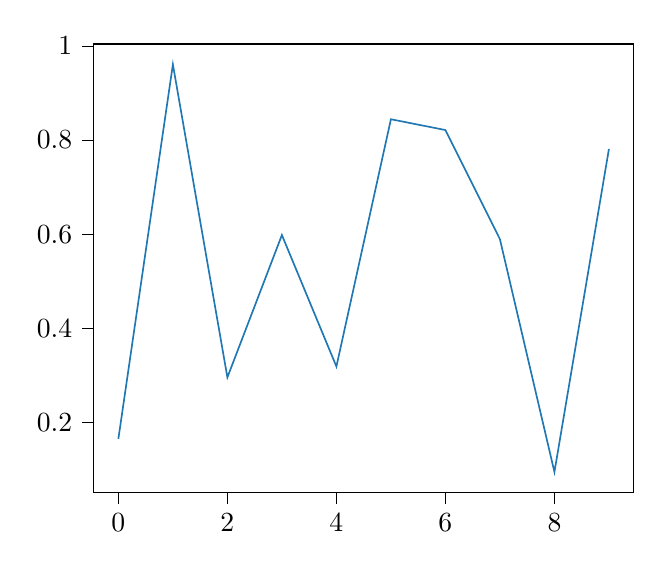
\begin{tikzpicture}

\definecolor{color0}{rgb}{0.12156862745098,0.466666666666667,0.705882352941177}

\begin{axis}[
tick align=outside,
tick pos=left,
x grid style={white!69.0196078431373!black},
xmin=-0.45, xmax=9.45,
xtick style={color=black},
y grid style={white!69.0196078431373!black},
ymin=0.0515297644926165, ymax=1.0037743262763,
ytick style={color=black}
]
\addplot [semithick, color0]
table {%
0 0.165204368712852
1 0.960490482558861
2 0.295706783168825
3 0.598084081751131
4 0.318814100655487
5 0.844017623549353
6 0.821076195130074
7 0.589191813076777
8 0.0948136082100567
9 0.781036863745426
};
\end{axis}

\end{tikzpicture}

%     \end{center}
%     \caption{A PGF histogram from \texttt{matplotlib}.}
% \end{figure}


% Advantage of compute shader.
% Maybe introduce cascaded Lowpass.



% All figures should be centred on the column (or page, if the figure spans both columns).
% Figure captions (in italic) should follow each figure and have the format given in Figure \ref{fft_plot}.
% %
% Vectorial figures are preferred. For example when using
% \texttt{Matlab}, export using either Postscript or PDF format. Also,
% in order to provide a better readability, figure text font size
% should be at least identical to footnote font size. To do so using
% \texttt{Matlab}, use the \texttt{subplot} command before plotting.
% If bitmap figures are used, please make sure that the resolution is
% enough for print quality. Fig. \ref{ftt_plot2} illustrates an
% example of a figure spanning two columns.
%


% \begin{figure}
%     \begin{center}
%       % This file was created by tikzplotlib v0.9.1.
\begin{tikzpicture}

\begin{axis}[
colorbar,
colorbar style={ylabel={}},
colormap={mymap}{[1pt]
  rgb(0pt)=(0.0000,0.0000,0.5000);
  rgb(22pt)=(0.0000,0.0000,1.0000);
  rgb(25pt)=(0.0000,0.0000,1.0000);
  rgb(68pt)=(0.0000,0.8600,1.0000);
  rgb(70pt)=(0.0000,0.9000,0.9677);
  rgb(75pt)=(0.0806,1.0000,0.8871);
  rgb(128pt)=(0.9355,1.0000,0.0323);
  rgb(130pt)=(0.9677,0.9630,0.0000);
  rgb(132pt)=(1.0000,0.9259,0.0000);
  rgb(178pt)=(1.0000,0.0741,0.0000);
  rgb(182pt)=(0.9091,0.0000,0.0000);
  rgb(200pt)=(0.5000,0.0000,0.0000)
},
point meta max=-55.7164,
point meta min=-100.0000,
tick align=outside,
tick pos=left,
width=0.8	extwidth,
x grid style={white!69.0196!black},
xlabel={Time [seconds]},
xmin=0.0231, xmax=0.0721,
xtick style={color=black},
y grid style={white!69.0196!black},
ylabel={Frequency [Hz]},
ymin=30.0000, ymax=5000.0000,
ytick style={color=black}
]
\addplot graphics [includegraphics cmd=\pgfimage,xmin=0.0231, xmax=0.0721, ymin=0.0000, ymax=22050.0000] {img/spec1-004.png};
\end{axis}

\end{tikzpicture}

%     \end{center}
%     \caption{\label{fig:shoe} \it Spec by this approach. Impulse response of shoebox room. Computed using the proposed method and \cite{lehmann_fast_2020}. }
    
% \end{figure}



% \begin{figure}
%     \begin{center}
%       % This file was created by tikzplotlib v0.9.1.
\begin{tikzpicture}

\begin{axis}[
colorbar,
colorbar style={ylabel={}},
colormap={mymap}{[1pt]
  rgb(0pt)=(0.0000,0.0000,0.5000);
  rgb(22pt)=(0.0000,0.0000,1.0000);
  rgb(25pt)=(0.0000,0.0000,1.0000);
  rgb(68pt)=(0.0000,0.8600,1.0000);
  rgb(70pt)=(0.0000,0.9000,0.9677);
  rgb(75pt)=(0.0806,1.0000,0.8871);
  rgb(128pt)=(0.9355,1.0000,0.0323);
  rgb(130pt)=(0.9677,0.9630,0.0000);
  rgb(132pt)=(1.0000,0.9259,0.0000);
  rgb(178pt)=(1.0000,0.0741,0.0000);
  rgb(182pt)=(0.9091,0.0000,0.0000);
  rgb(200pt)=(0.5000,0.0000,0.0000)
},
point meta max=-54.1665,
point meta min=-100.0000,
tick align=outside,
tick pos=left,
width=0.8	extwidth,
x grid style={white!69.0196!black},
xlabel={Time [seconds]},
xmin=0.0231, xmax=0.0721,
xtick style={color=black},
y grid style={white!69.0196!black},
ylabel={Frequency [Hz]},
ymin=30.0000, ymax=5000.0000,
ytick style={color=black}
]
\addplot graphics [includegraphics cmd=\pgfimage,xmin=0.0231, xmax=0.0721, ymin=0.0000, ymax=22050.0000] {img/orig-003.png};
\end{axis}

\end{tikzpicture}

%     \end{center}
%     \caption{\label{fig:shoe} \it Spec by matlab. Impulse response of shoebox room. Computed using the proposed method and \cite{lehmann_fast_2020}. }
    
% \end{figure}


% \begin{figure}
%     \begin{center}
%       % This file was created by tikzplotlib v0.9.1.
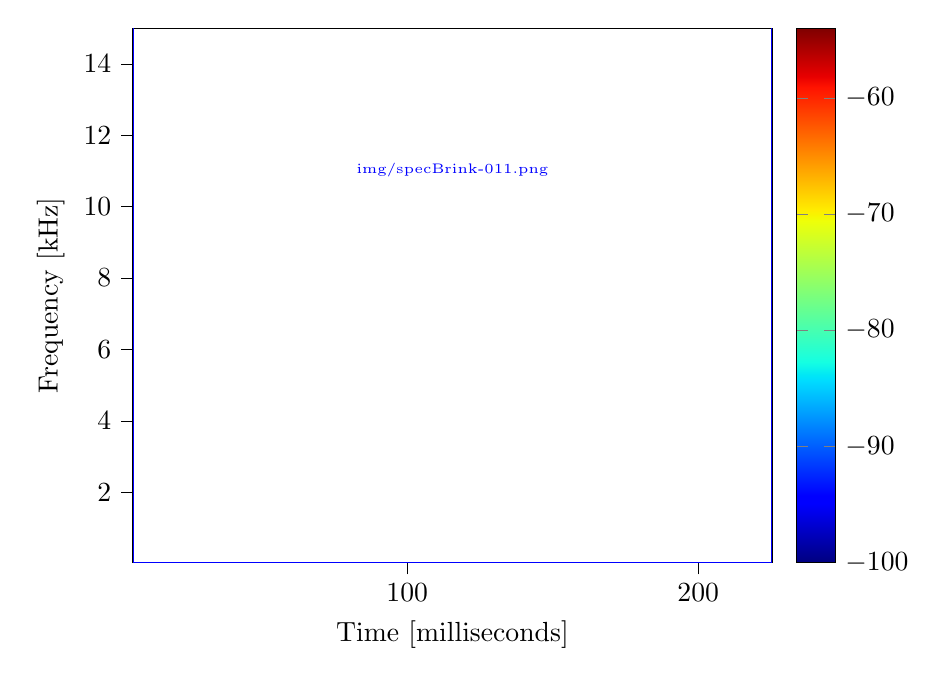
\begin{tikzpicture}

\begin{axis}[
colorbar,
colorbar style={ylabel={}, y label style={yshift=1.5em}},
colormap={mymap}{[1pt]
  rgb(0pt)=(0.0000,0.0000,0.5000);
  rgb(22pt)=(0.0000,0.0000,1.0000);
  rgb(25pt)=(0.0000,0.0000,1.0000);
  rgb(68pt)=(0.0000,0.8600,1.0000);
  rgb(70pt)=(0.0000,0.9000,0.9677);
  rgb(75pt)=(0.0806,1.0000,0.8871);
  rgb(128pt)=(0.9355,1.0000,0.0323);
  rgb(130pt)=(0.9677,0.9630,0.0000);
  rgb(132pt)=(1.0000,0.9259,0.0000);
  rgb(178pt)=(1.0000,0.0741,0.0000);
  rgb(182pt)=(0.9091,0.0000,0.0000);
  rgb(200pt)=(0.5000,0.0000,0.0000)
},
point meta max=-54.0062,
point meta min=-100.0000,
tick align=outside,
tick pos=left,
width=0.8\textwidth,
x grid style={white!69.0196!black},
xlabel={Time [milliseconds]},
xmin=0005.7, xmax=225.4,xtick={0, 100,200},
xtick style={color=black},
y grid style={white!69.0196!black},
ylabel={Frequency [kHz]},
ymin=0.0300000, ymax=15.0000000,
ytick style={color=black}
]
\addplot graphics [includegraphics cmd=\pgfimage,xmin=5.7, xmax=225.4, ymin=0.0000, ymax=22.0500000] {img/specBrink-011.png};
\end{axis}

\end{tikzpicture}

%     \end{center}
%     \caption{\label{fig:shoe} \it Original \cite{brinkmann_round_2019}. }
    
% \end{figure}


% \begin{figure}
%     \begin{center}
%       % This file was created by tikzplotlib v0.9.1.
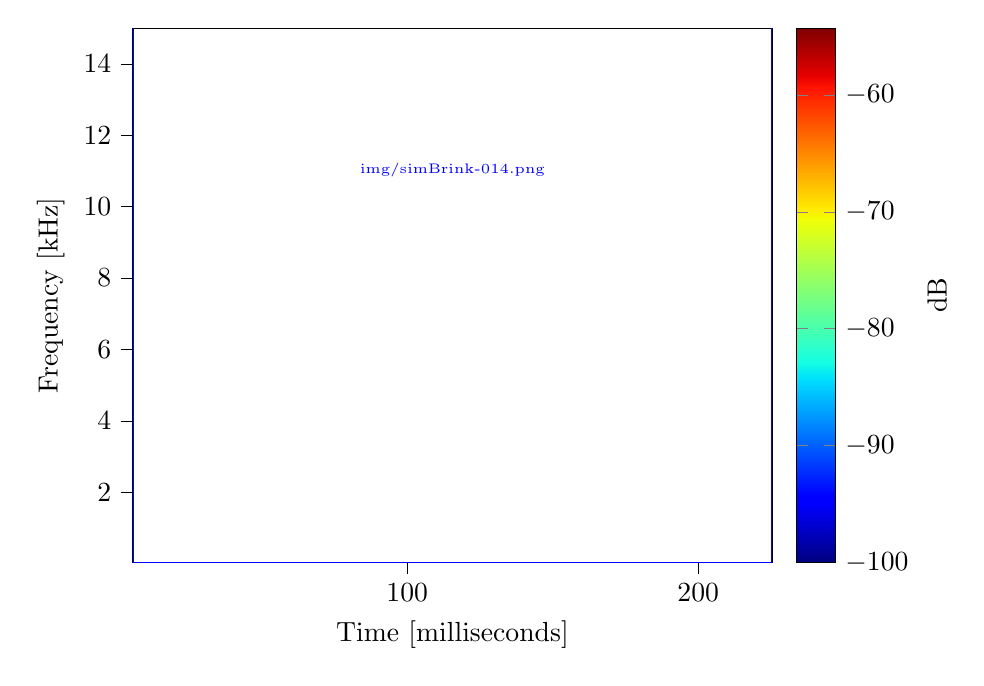
\begin{tikzpicture}

\begin{axis}[
colorbar,
colorbar style={ylabel={dB}},
colormap={mymap}{[1pt]
  rgb(0pt)=(0.0000,0.0000,0.5000);
  rgb(22pt)=(0.0000,0.0000,1.0000);
  rgb(25pt)=(0.0000,0.0000,1.0000);
  rgb(68pt)=(0.0000,0.8600,1.0000);
  rgb(70pt)=(0.0000,0.9000,0.9677);
  rgb(75pt)=(0.0806,1.0000,0.8871);
  rgb(128pt)=(0.9355,1.0000,0.0323);
  rgb(130pt)=(0.9677,0.9630,0.0000);
  rgb(132pt)=(1.0000,0.9259,0.0000);
  rgb(178pt)=(1.0000,0.0741,0.0000);
  rgb(182pt)=(0.9091,0.0000,0.0000);
  rgb(200pt)=(0.5000,0.0000,0.0000)
},
point meta max=-54.2825,
point meta min=-100.0000,
tick align=outside,
tick pos=left,
width=0.8\textwidth,
x grid style={white!69.0196!black},
xlabel={Time [milliseconds]},
xmin=005.7, xmax=225.4,xtick={100, 200},
xtick style={color=black},
y grid style={white!69.0196!black},
ylabel={Frequency [kHz]},
ymin=0.0300000, ymax=15.0000000,
ytick style={color=black}
]
\addplot graphics [includegraphics cmd=\pgfimage,xmin=5.7, xmax=225.4, ymin=0.0000, ymax=22.0500000] {img/simBrink-014.png};
\end{axis}

\end{tikzpicture}

%     \end{center}
%     \caption{\label{fig:shoe} \it Simulated. }
    
% \end{figure}

% \begin{enumerate}



% Eric A. Lehmann (2020). Fast simulation of acoustic room impulse responses (image-source method) (https://www.mathworks.com/matlabcentral/fileexchange/25965-fast-simulation-of-acoustic-room-impulse-responses-image-source-method), MATLAB Central File Exchange. Retrieved February 14, 2020.

% \end{enumerate}


% \begin{figure}[ht]
% \centerline{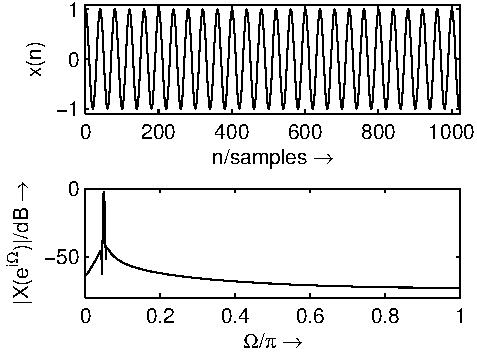
\includegraphics[scale=0.8]{fft_plot2}}
% \caption{\label{fft_plot}{\it Sinusoid in time and frequency domain. Short captions are centred, long captions (more than 1 line) are justified.}}
% \end{figure}
% %
% \begin{figure*}[ht]
% \center
% 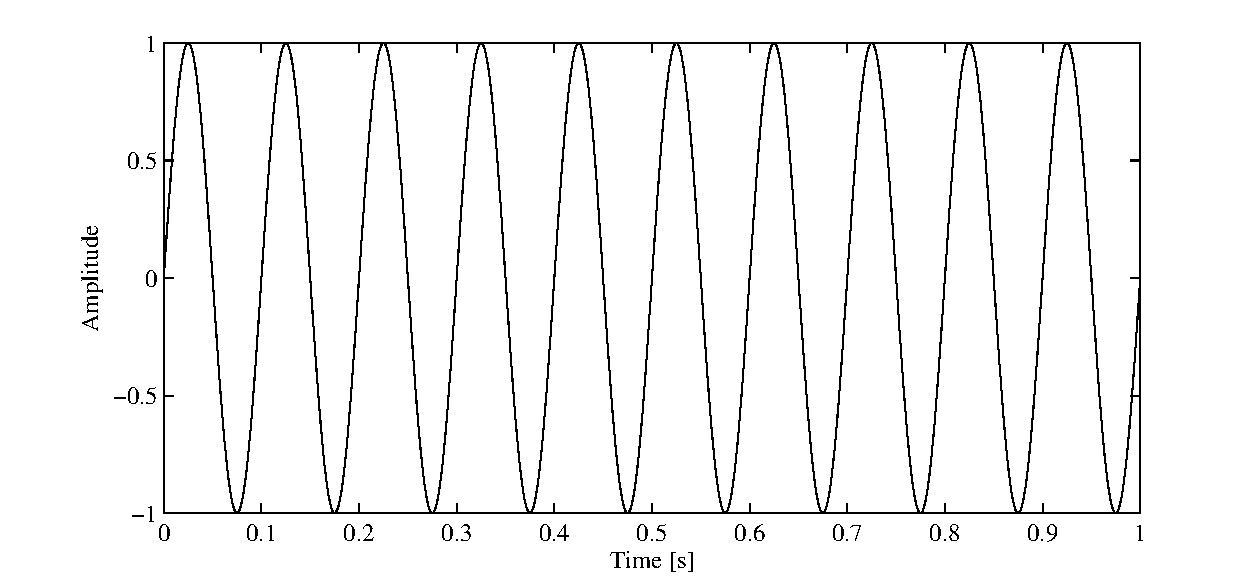
\includegraphics[width=5in]{TwoColumnSine2}
% \caption{\label{ftt_plot2}{\it A figure spanning two columns, as mentioned in Sec. . }}
% \end{figure*}


% \begin{figure}[ht]
% \centerline{\includegraphics[scale=0.8]{img/test1.pgf}}
% \caption{\label{fft_plot}{\it Sinusoid in time and frequency domain. Short captions are centred, long captions (more than 1 line) are justified.}}
% \end{figure}

% \begin{figure}
%     \begin{center}
%       % This file was created by tikzplotlib v0.9.1.
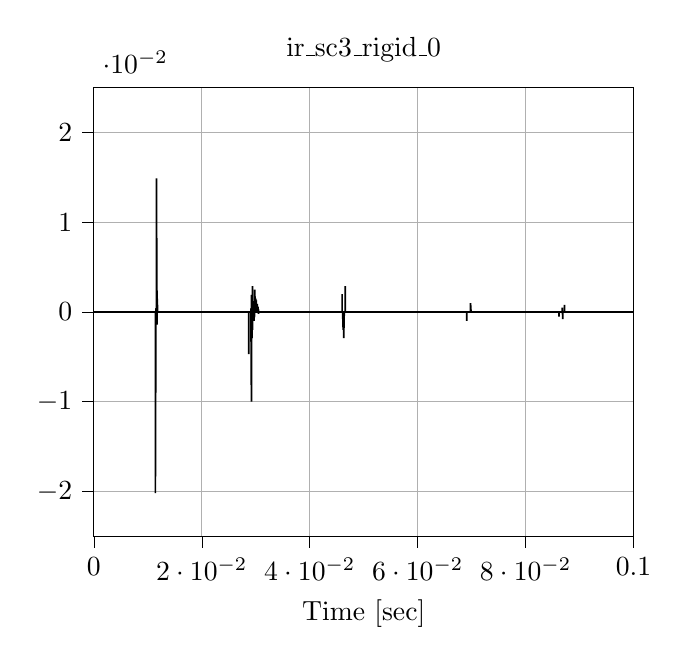
\begin{tikzpicture}

\begin{axis}[
tick align=outside,
tick pos=left,
title={ir\_sc3\_rigid\_0},
x grid style={white!69.0196!black},
xlabel={Time [sec]},
xmajorgrids,
xmin=0.0000, xmax=0.1000,
xtick style={color=black},
y grid style={white!69.0196!black},
ymajorgrids,
ymin=-0.0250, ymax=0.0250,
ytick style={color=black}
]
\addplot [semithick, black]
table {%
0.0000 0.0000
0.0114 0.0000
0.0114 -0.0202
0.0115 0.0000
0.0115 0.0000
0.0115 0.0000
0.0115 0.0001
0.0116 0.0000
0.0116 0.0001
0.0116 0.0149
0.0117 -0.0014
0.0117 0.0024
0.0117 0.0003
0.0117 0.0020
0.0118 0.0005
0.0118 0.0000
0.0121 0.0000
0.0287 0.0000
0.0287 -0.0047
0.0287 0.0000
0.0291 0.0000
0.0291 0.0004
0.0292 -0.0100
0.0292 0.0019
0.0292 -0.0009
0.0292 -0.0006
0.0293 0.0004
0.0293 -0.0001
0.0293 -0.0000
0.0293 0.0004
0.0293 -0.0029
0.0294 0.0029
0.0294 -0.0020
0.0294 0.0018
0.0295 -0.0001
0.0295 0.0000
0.0295 0.0009
0.0295 -0.0009
0.0295 0.0012
0.0296 -0.0004
0.0296 0.0000
0.0296 -0.0005
0.0297 0.0010
0.0297 -0.0010
0.0297 0.0011
0.0297 -0.0008
0.0298 0.0013
0.0298 -0.0005
0.0298 0.0025
0.0299 0.0009
0.0299 0.0012
0.0299 0.0007
0.0300 0.0011
0.0300 0.0007
0.0300 -0.0001
0.0300 0.0015
0.0300 0.0005
0.0301 0.0007
0.0301 0.0004
0.0301 0.0008
0.0302 0.0004
0.0302 0.0008
0.0302 0.0002
0.0302 0.0007
0.0303 0.0006
0.0303 -0.0001
0.0303 0.0009
0.0303 -0.0000
0.0304 0.0006
0.0304 0.0004
0.0304 0.0000
0.0304 0.0006
0.0305 -0.0002
0.0305 0.0003
0.0305 0.0000
0.0460 0.0000
0.0460 0.0020
0.0460 -0.0000
0.0461 -0.0000
0.0462 -0.0020
0.0462 0.0000
0.0463 0.0000
0.0463 -0.0029
0.0464 -0.0000
0.0465 0.0000
0.0466 0.0000
0.0466 0.0029
0.0466 0.0000
0.0691 0.0000
0.0691 -0.0010
0.0691 0.0000
0.0698 0.0000
0.0698 0.0010
0.0699 0.0000
0.0862 0.0000
0.0862 -0.0005
0.0862 0.0000
0.0868 0.0000
0.0868 0.0005
0.0869 -0.0008
0.0869 0.0000
0.0872 0.0000
0.0872 0.0008
0.0872 0.0000
0.1000 0.0000
};
\end{axis}

\end{tikzpicture}

%         % % This file was created by tikzplotlib v0.9.1.
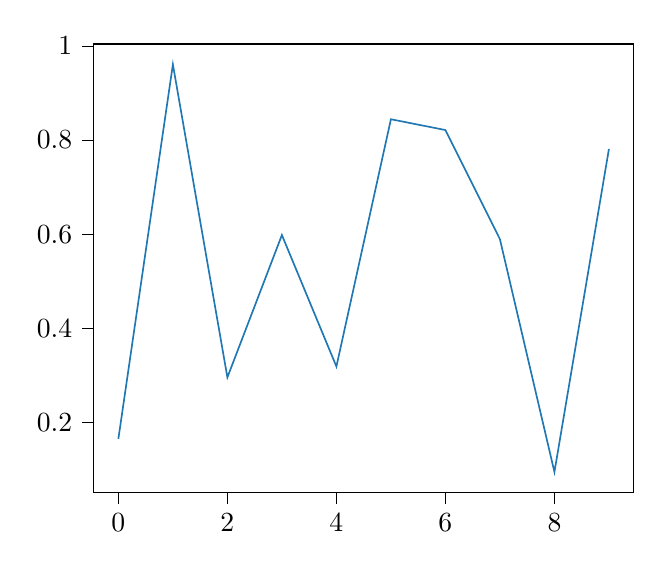
\begin{tikzpicture}

\definecolor{color0}{rgb}{0.12156862745098,0.466666666666667,0.705882352941177}

\begin{axis}[
tick align=outside,
tick pos=left,
x grid style={white!69.0196078431373!black},
xmin=-0.45, xmax=9.45,
xtick style={color=black},
y grid style={white!69.0196078431373!black},
ymin=0.0515297644926165, ymax=1.0037743262763,
ytick style={color=black}
]
\addplot [semithick, color0]
table {%
0 0.165204368712852
1 0.960490482558861
2 0.295706783168825
3 0.598084081751131
4 0.318814100655487
5 0.844017623549353
6 0.821076195130074
7 0.589191813076777
8 0.0948136082100567
9 0.781036863745426
};
\end{axis}

\end{tikzpicture}

%     \end{center}
%     \caption{A PGF histogram from \texttt{matplotlib}.}
% \end{figure}




% \subsection{Tables}
% As for figures, all tables should be centered on the column (or page, if the table spans both columns).
% Table captions should be in italic, precede each table and have the format given in Table \ref{tab:example}.

% \begin{table}[ht]
%   \caption{\itshape Basic trigonometric values.}
%   \centering
%   \begin{tabular}{|c|c|}
%     \hline
%     $\mathrm{angle}\,(\theta, \mathrm{rad})$ & $\sin \theta$ \\\hline
%     $\frac{\pi}{2}$ & $1$ \\
%     $\pi$ & $0$ \\
%     $\frac{3\pi}{2}$ & $-1$ \\
%     $2\pi$ & $0$ \\\hline
%   \end{tabular}
%   %
%   \label{tab:example}
% \end{table}

% \begin{table*}[ht]
%   \caption{{\it Basic trigonometric values, spanning two columns.}}
%   \centering
%   \begin{tabular}{|c|c|c|c|c|c|c|}\hline
%     $\mathrm{angle}\, (\theta, \mathrm{rad})$ & $\sin \theta$ & $\cos \theta $ & $(\sin \theta)/2 $ & $(\cos \theta) /2 $ & $(\sin \theta)/3 $ & $(\cos \theta)/3$    \\\hline
%     $\frac{\pi}{2}$ & $1$ & $0$ & $1/2$ & $0$ & $1/3$ & $0$ \\
%     $\pi$ & $0$ & $-1$ & $0$ & $-1/2$ & $0$ & $-1/3$\\
%     $\frac{3\pi}{2}$ & $-1$ & $0$ & $-1/2$ & $0$ & $-1/3$ & $0$ \\
%     $2\pi$ & $0$ & $1$ & $0$ & $1/2$ & $0$ & $1/3$ \\\hline
%  \end{tabular}
%   %
%   \label{tab:example2}
% \end{table*}

% \subsection{Equations}
% Equations should be placed on separate lines and numbered:

% \begin{equation}
%   X(e^{j\Omega})=\sum_{n=0}^{N-1}x(n)e^{-j\Omega n}
%   \label{eq1}
%   \end{equation}
%   where the sequence $x(n)$ in equation (\ref{eq1}) is a windowed frame:
%   \begin{equation}
%   x(n)=s(n) w(n)
%   \label{eq2}
% \end{equation}
% %
% with a window function $w(n)$.
